%% LyX 2.3.7 created this file.  For more info, see http://www.lyx.org/.
%% Do not edit unless you really know what you are doing.
\documentclass[12pt,english]{article}
\usepackage[T1]{fontenc}
\usepackage[latin9]{inputenc}
\usepackage{geometry}
\geometry{verbose,tmargin=1cm,bmargin=2cm,lmargin=3cm,rmargin=3cm,headheight=3cm,headsep=3cm,footskip=1.2cm,columnsep=1.2cm}
\usepackage{array}
\usepackage{float}
\usepackage{mathrsfs}
\usepackage{multirow}
\usepackage{amsmath}
\usepackage{amsthm}
\usepackage{amssymb}
\usepackage{graphicx}
\usepackage{setspace}
\PassOptionsToPackage{normalem}{ulem}
\usepackage{ulem}
\onehalfspacing

\makeatletter

%%%%%%%%%%%%%%%%%%%%%%%%%%%%%% LyX specific LaTeX commands.
%% Because html converters don't know tabularnewline
\providecommand{\tabularnewline}{\\}

%%%%%%%%%%%%%%%%%%%%%%%%%%%%%% Textclass specific LaTeX commands.
\theoremstyle{plain}
    \ifx\thechapter\undefined
      \newtheorem{assumption}{\protect\assumptionname}
    \else
      \newtheorem{assumption}{\protect\assumptionname}[chapter]
    \fi

%%%%%%%%%%%%%%%%%%%%%%%%%%%%%% User specified LaTeX commands.
\usepackage[T1]{fontenc}
\usepackage{tgtermes}
\usepackage{mathtools}
\usepackage{amsmath}
\usepackage{xparse}
\usepackage{lscape}
\usepackage[section]{placeins}
\usepackage{apacite}
\usepackage{etoolbox}
\patchcmd{\thebibliography}{\section*{\refname}}{}{}{}


\usepackage{titlesec}
\usepackage{bbm}


\usepackage{longtable}
\usepackage{booktabs}
\usepackage{sectsty}
\tolerance=1
\emergencystretch=\maxdimen
\hyphenpenalty=10000
\hbadness=10000

\usepackage{color, colortbl}
\usepackage[first=0,last=9]{lcg}
\usepackage[left,modulo]{lineno}


\usepackage{soul}
\usepackage{color}

\usepackage[absolute]{textpos}


\newcommand{\hlc}[1]{{\sethlcolor{LightCyan}\hl{#1}}}
\newcommand{\hly}[1]{{\sethlcolor{LightYellow}\hl{#1}}}
\newcommand{\hlw}[1]{{\sethlcolor{White}\hl{#1}}}
\newcommand{\hlg}[1]{{\sethlcolor{LightGreen}\hl{#1}}}

\definecolor{Gray}{gray}{0.9}
\definecolor{LightCyan}{rgb}{0.88,1,1}
\definecolor{LightYellow}{RGB}{255,255,200}
\definecolor{LightGreen}{RGB}{204,255,204}
\definecolor{White}{RGB}{255,255,255}
\newcommand{\ra}{\rand0.\arabic{rand}}


\makeatletter
\@addtoreset{section}{part}
\def\@part[#1]#2{%
    \ifnum \c@secnumdepth >\m@ne
      \refstepcounter{part}%
      \addcontentsline{toc}{part}{\thepart\hspace{1em}#1}%
    \else
      \addcontentsline{toc}{part}{#1}%
    \fi
    {\parindent \z@ \raggedright
     \interlinepenalty \@M
     \normalfont\centering
     \ifnum \c@secnumdepth >\m@ne
       \large\bfseries \partname\nobreakspace\thepart
       \par\nobreak
     \fi
     \huge \bfseries #2%
     \markboth{}{}\par}%
    \nobreak
    \vskip 3ex
    \@afterheading}
\renewcommand\partname{Topic}
\makeatother

\makeatother

\usepackage{babel}
\providecommand{\assumptionname}{Assumption}

\begin{document}
\pagenumbering{gobble}
\partfont{\fontsize{20}{22}\selectfont\centering} 
\part*{\centering{The Role of Income Inequalities in Aspirational Consumption}}

\rule{1\columnwidth}{1pt}

\begin{textblock*}{7.8in}(3.0cm,4.1cm) % (column-position,row-position) 
\begin{minipage}{0.72\textwidth} 
\begin{center}{\textbf{Summary} }\end{center}

\hlw{The presented study explores reported rises in aspirational
consumption in the developing economies and asks whether such a rise
may be subject to a leveling effect seen in developed economies or
not. Viewing status consumption in a generic context, the study assumes
an explicit link between status goals and economic goals of the consumer.
The empirical analyses then assess possible rises in consumption by
examining the role of household permanent income on food and education
- both of which are observed to carry a status value in sub-Saharan
Africa. The three chapters in the study draw a set of independent
conclusions on effects of inequality on status consumption. The equilibrium
conditions discussed in the first theoretical chapter for a model
of status as a position hierarchy where consumers are able to move
between through social capital investments reveal that positional
contests can become uncompetitive with a rise in income inequality.
This first chapter highlights two types of long-term equilibria where
either only rich consumers participate in status competitions or both
rich and poor participate. The empirical second chapter explores the
role of household permanent income on food quality in Tanzania to
observe that permanent income - alongside with availability of electricity
in the country - may have a segregating effect on food quality. The
third chapter compares education expenses in Nigeria and Tanzania
- finding that education expenses in Nigeria are more significantly
influenced by local wealth levels than permanent income. In light
of the two long-term equilibria discussed in the first chapter, the
study highlights how a rise in expenditure on status items as a common
need may contribute to rise in status consumption in developing economies
when the consumption of such items is linked with perceptions of mobility.}

\end{minipage}
\end{textblock*}%

\newpage

\tableofcontents{}

\newpage

\pagenumbering{arabic}

%%%%%%%%%%%%%%%%%%%%%%%%%%%%%%%%%%%%%%%%%%%%%%%%%%%%%%%%%%%%%%%%%%%%%%%%%%%%%%%%%%%%%%%%%%%%%%%%%%%%%%%%%%%%%%%%%%%%%%%%%%%%%%%%%%%%%%%%%%%%%%%%%%%%%%%%%%
%%%%%%%================================== PASTE ALL CHAPTERS BELOW ==============================================
%%%%%%%%%%%%%%%%%%%%%%%%%%%%%%%%%%%%%%%%%%%%%%%%%%%%%%%%%%%%%%%%%%%%%%%%%%%%%%%%%%%%%%%%%%%%%%%%%%%%%%%%%%%%%%%%%%%%%%%%%%%%%%%%%%%%%%%%%%%%%%%%%%%%%%%%%%

\partfont{\fontsize{14}{16}\selectfont\centering} 
\part{\centering{Preface}} \label{part:preface}

\noindent

\hlw{At a time when developing economies strive to improve per-capita
life-standards, studies have also highlighted an increasing role of
aspirational consumption} \cite{TimothyBurkeLifebuoyMen1996,SrivastavaMukherjee2020aspcon,MoavNeeman2012savingandpoverty}.
\hlw{ Aspirational consumption is commonly understood as consumption
relevant for status signaling needs or social aspirations - but not
only are the empirical tests of visible consumption across developing
economies sensitive to extreme variation in cultural contexts, the
very idea that visible consumption is wasteful may also deserve scrutiny
if a rising affluence of societies transitioning away from subsistence
lifestyles (or endogenous growth) raises common needs across the society. 

Such a rise in common needs could be both due to a rise in quality
of basic consumption (such as food, clothing) and with an introduction
of newer goods into the consumer basket. It is not surprising thus
that on one hand, the literature on aspirational consumption finds
aspirational consumption to form a pathway to a brighter future}
\cite{SrivastavaMukherjee2020aspcon,jaikumar2018showoff,BanerjeeDufloPoorEcon}
\hlw{ but on the other, it is also suggested that consumers stretch
their budgets on basic needs to address compensatory aspirational
consumption }\cite{KausSA,ZahraIndia,roychowdhuryInequalityStatusConsumption2016}.
\hlw{Addressing the specific concern of what may constitute status
consumption in a developing economy, the presented study focuses on
two shortcomings of the prevalent view of rise in aspirational consumption
in order to answer how inequalities influence the rise in aspirational
consumption. First, it revisits the sociological basis for status
in order to consider a broader view of status-related consumption
than what is permitted with the notion of visible consumption. Second,
it considers mobility perceptions as a potential factor for consumption
changes in an environment of wide income differences. It is by addressing
both of these issues that the thesis attempts to answer how inequalities
may contribute to a rise in aspirational consumption.

The two issues pertaining to aspirational consumption amidst inequalities
are particularly relevant to SSA - first since a recent urbanisation
of the region may allow for status indication though higher quality
or newer consumption types and second, since recent economic growth
may prioritise mobility and its perceptions - resulting in the seemingly
``futile'' }\cite{VeblenLeisureClass} \hlw{consumption becoming
a social need with material consequences for the consumer. Drawing
from the sociological literature for status }\cite{wegener1992prestigeconcepts},
\hlw{the presented study links consumption with notions of aspiration
to provide theoretical arguments for how aspirational consumption
could change under income inequalities in developing economies. The
empirical chapters in the study then examine distribution of consumption
pertaining to status with respect to permanent income in SSA.

We argue that the idea of certain goods carrying a visible appeal
has often been embraced in the developing economies without examining
the historical and cultural settings that might influence status perceptions
in an economy }\cite{nieftagodien2007blacksconsumption,Burger2015SAMiddleClass}.
\hlw{The interpretations of status signaling mechanisms in the developing
world also ignore that widespread poverty tends to make seemingly
necessary items carry status significance as well. The expenditures
such as education - for example - have been treated as a necessity
despite the literature finding some evidence of rent-seeking }\cite{buchertEducTNZ1992,BabalolaFinancingEducationinNigeria1998,FilmerPritchettWealthEffectonEduc1999,BarrHEFunding2004,NdyaliHE_Unemployment_TNZ2016,AllaisMeasuringHEValueinSA2017,EbaidallaSudanHHeducExpenditure2018}
or eliteness \cite{MinnisNonformalEducation2006} \hlw{from educational
degrees. Conversely, while consumption of clothing or personal products
- regardless of variation in quality - are commonly considered visible
consumption} \cite{KausSA,ZahraIndia,roychowdhuryInequalityStatusConsumption2016}
\hlw{in the developing economies, the literature also points to the
necessity of such consumption by finding evidence of improvement in
subjective well-being }\cite{linssen2011subjectivewellbeingIndia,guillen2011referencecons}.\hlw{
A more general view of aspirational consumption adopted in the study
attempts to highlight how some of the claims of unusual or prominent
urges towards aspirational consumption among the poor developing economies
}\cite{subrahmanyanBoPConsumption2008,SrivastavaMukherjee2020aspcon}
\hlw{- may in part be due to the lack of an established standard
for maximal level of common needs in an economy. With there being
well-known issues with a direct measurement of necessities of consumers
}\cite{SenRejoinderTownsend1985,TownsendRejoinderSen1985,DoyalGoughNeeds1991},\hlw{
the attribution of higher consumption to aspirational needs might
be appropriate in a normative sense, but frequent attributions of
higher or lower wastefulness to specific sections of society require
one to reconcile the sociological basis for status needs in an economy
as well - thus considering both the dynamics of status in the economy
and the notion of wastefulness associated with certain consumption.
}

In a theoretical exploration of how income differences may influence
aspirational consumption (in a more general sense than what is implied
by visible consumption), we focus firstly on a particular social value
that the consumer may derive from aspirational consumption. Drawing
from the literature on status in sociology \cite{webereconomysociety1925,goode1978celebrationheroes,wegener1992prestigeconcepts},
the theoretical first chapter assumes a specific link between economic
and social goals of the individual to explain effect of income-inequalities
on consumption - which are viewed as investments towards social capital
needed to pursue social positions. The empirical chapters then proceed
to examine the distribution of exclusive and high-quality consumption
that have been reported to carry status advantage in SSA but do not
fall under visible goods category.

It is worth elaborating how the above view of aspirational consumption
contrasts against that of conspicuous consumption as futile splurges
of the rich \cite{VeblenLeisureClass} and how it motivates our exploration
of income inequality effects. The distinction between the view of
conspicuous consumption as splurges of the rich and that of a generalised
status consumption is an important one since if high-priced consumption
were to be limited only to those with higher income or wealth, then
there are evident limits implied for the rise of such consumption
\cite{HirschSocialLimits}. In other words, the high-priced consumption
- if limited to richer sections - is subject to how extreme income
inequalities persist in the economy - since such consumption may rise
only as much as the proportion of rich rises in a population. Therefore
if aspirational consumption is strictly interpreted as trophies of
the rich or as futile attempts to emulate the rich, then such consumption
is necessarily limited to the rich and its purported rise cannot be
widespread in an unequal society. With a more general view of aspirational
consumption taken in the study on the other hand, the scope of aspirational
consumption is necessarily wider as it concerns itself with how aspirational
consumption may expand to the masses as a common need. The general
view of aspirational consumption combined with the link between economic
and social goals allows us to interpret the effects of mobility concerns
on consumption as investments towards social capital towards economic
gains \cite{goode1978celebrationheroes,HirschSocialLimits} for the
consumer. As we further explain, such a general view may be better
suited to reconciling the sociological bases for status in an economy.

% Such a view of aspirational consumption does not make any claims on the consumer's intent in purchase of a specific item (i.e. whether education or food is a status item in some sense or not) - a concern that is fundamentally a descriptive one and one that the analysis of household diary data alone may not address.
% We focus on the role of secondary-schools rather than tertiary-level schools as the latter is much rarer in the poorer of the two economies (Tanzania) to allow an admissible comparison of expenses in the two economies.

The empirical chapters in the study do not assume the existence of
purely visible items and consider two ways in which high-consumption
of status relevance can be availed in the cross-section of a typical
sub-Saharan economy. The first type of consumption is one that can
be viewed as a higher quality of a commonly consumed basic good. The
second type is one that is altogether exclusive to the richer sections
i.e. inaccessible to the vast majority. The primary distinction between
the two-types of consumption in the study is an empirical one wherein
the quality variation is relevant for the first type of consumption
and it isn't for the second type. The rationale behind this distinction
is that in a generic sense of status signaling (rather the one implied
by futile goods alone), the available quality in the market makes
it possible for a richer consumer to distinguish herself from the
poorer consumer while an item with less lower-quality variants may
be relevant for status purposes only through the poor being priced
of purchasing such an item. One can hardly dispute that food is a
basic necessity but there also seems evidence for status-indication
through food quality in developing economies (e.g., for Tanzania\cite{ohna2007foodstatus,ohna2012nofoodwougali}).
Mass Education, on the other hand, is quite unlike food and is a relatively
newer consumption type in SSA - with an evidence for its status value
as well \cite{MinnisNonformalEducation2006,porzio2021human}. 

The first empirical chapter in the study inspects variation in food
quality in Tanzania - which presents itself as an economy where rapid
changes in consumption patterns have been highlighted under recent
urban developments. The second empirical chapter compares education
expenses in a rural economy with a relatively more urbanised one by
selecting Tanzania and Nigeria - which are countries with disparate
levels of industrial dependence. It is worth highlighting that all
consumption - regardless of high or low quality - is surveyed across
the cross-section in both the empirical chapters. Since consumption
being limited a rich household must evidently limit the long-term
rise in overall consumption in the economy, the role of household
permanent-income is explored in both the empirical chapters so as
to comment on possible future rises in consumption.

As such, many different scenarios may arise with food and education
considered as the two types of aspirational consumption. With food
quality, one could find that budget shares for food quality do not
vary much across the population (as is the case for only a few specific
food items) or that high food quality is severely limited to richer
households. Similarly, with respect to education - which is more exclusive
relative to food - one may find that it is affordable only to rich
households or that it's availed across all income levels. A comparison
of education expenses in Tanzania and Nigeria suggests that education
is distributed across the population in asset-rich regions whereas
a view of distribution of food quality in Tanzania shows that high
quality is significantly limited to richer and urban households. The
role of household permanent income appears to be less important for
education in urbanised areas than for high quality food - suggesting
how certain types of consumption - subject to changes in economic
growth - are more likely to become a growing need in the population.
These observations can be viewed in light of the theoretical findings
of the first chapter on how persistent household income inequalities
influence demand for status-goods varying in their potential mobility
value. As we detail in the study and discuss further in the epilogue
(Part \ref{part:epilogue}), education may be different from food
not only through being a newer type of consumption category in the
rural economies (which also allows the variation in quality to be
of a less empirical concern) but also in how it may relate to future
economic gains. A view of expenditures sensitive to perceptions of
mobility (e.g., education ) that considers status neither a purely
conspicuous concern nor a necessity may be better equipped to explaining
upward pressures on certain aspects of aspirational consumption.

% (WHAT ABOUT TAUTOLOGICAL VIEW OF HIGH QUALITY BEING LIMITED TO RICHER HOUSEHOLDS - one solution is that we highlight urban effects more)

%[FINDINGS]

To sum up, a theoretical chapter in the presented study finds that
long-term socio-economic income inequalities limit competitions for
status even though such investments (i.e. aspirational consumption)
rise with an increase in inequality in the short-term. The empirical
assessments then find that while high expenditure for certain items
may be limited to those with higher permanent income, the urbanisation-related
changes could have an effect of reducing the role of household permanent
income on expenditure for certain consumption categories (while also
creating wider differences between urbanised and rural areas). That
richer consumers (those with higher wealth and/or income) are likely
to have better access to higher quality goods and items that are out
of reach for the masses is less surprising, but whether such consumption
is likely to be limited to the richer sections of the society in an
environment of wide differences in wealth and income levels depends
much on the type of value the particular consumption may provide to
the consumer rather than on notions of wastefulness - especially when
the notions are not validated as a part of the status dynamics of
an economy. The presented study urges more focus on mobility perceptions
as such a value - which ought to be taken into account when examining
changes in consumption in developing economies.

%%%%%%%%%%%%%%%%%%% CHAPTER 1 %%%%%%%%%%%%%%%%%%%%%%%

\pagebreak

\partfont{\fontsize{14}{16}\selectfont\centering} 
\part{\centering{Status concerns and consumption under Income Inequality}}

\vspace{1.5in}

\begin{abstract}
Status motivations for consumption have generated an immense interest
at a time when social mobility has been relatively stagnant - but
the consequences of inequality within societies on patterns of development
are still poorly understood. To explain status motivations under environments
of income inequality, we treat opportunities for mobility as a link
between economic and social goals of the individual and view the consumption
as investments towards future economic success. Considering an economy
with a dynamic hierarchy of rich and poor positions that consumers
are able to move between, we then ask how relative incomes associated
with each position may influence the agents\textquoteright{} consumption
or labour supply decisions. With a diminishing returns to utility
from wealth optimised by a consumer endowed with randomly distributed
success-determining attributes and the promotion probabilities depending
on her expenditure, we find that a rise in income inequality provides
more incentive to participate in status competitions. With consumers
bearing the participation costs for mobility, the long-term equilibrium
conditions suggest two states - one where both rich and poor strive
for status and the other where only the rich consumers participate
in status competitions.
\end{abstract}

\section{Introduction}

\noindent

%[The QUESTION]

The consumer response to relative income has appealed to economists
since at least as far back as \citeA{VeblenLeisureClass}. While the
post-war period of relative stability and life-style improvements
have renewed an interest in the positional concerns \cite{FrankPond,HirschSocialLimits},
there remains a disconnect between descriptive theories for relative
income effects and theories of economic growth (see \cite{KayRadicalUncertainty2020,SanjitDhamiBehavioural2016}).
In the context of aspirational consumption in the developing economies,
such a disconnect makes it difficult to argue whether rises in aspirational
consumption are a mere consequence of social shifts pertaining to
growth and income redistribution in the economy or not. As the economies
may vary significantly across institutional efficacy and socio-political
environments, a prediction of rise in aspirational consumption is
problematic unless one relies upon a well-defined mechanism relating
relative income concerns and growth in the economy. We argue that
a view of status goals as independent of economic concerns may not
offer a satisfactory view of aspirational concerns in the developing
economies. Our appraoch uses a specific link between economic and
social goals instead to answer the questions pertaining to effects
on income inequality on aspirational consumption. The presented chapter
focuses on a context of aspirational consumption where it can be treated
as investments towards mobility and then asks whether such investments
should increase or decrease with a rise in income inequality.

Such a view of status adds a particular dynamism to the predominant
view of status as a hierarchy of ranks \cite{goldthorpeOccupationalGrading1975,wegener1992prestigeconcepts,goldthorpesociology2000}.
In viewing status competitions as games that provide direct gains
to the consumer as probabilistic economic rewards pertaining to status,
the current chapter takes cue from several attempts in both sociology
and economics that have argued for a more dynamic framework for status
\cite{webereconomysociety1925,shilsDeference1969,parsonssystemsocieties1971,ColemanSocialTheory1990,wegener1992prestigeconcepts}.
The presented approach pins down a specific link between economic
and social goals relevant for status consumption by assuming an indirect
(instrumental) effect of status on consumer wealth \cite{ColeMaliathSocialNorms1992,postlewaite1998socialbasisinterdeppreferences}.
While such a link may not have been of relevance to many empirical
studies on visible consumption \cite{heffetz_visibility,ireland_signals,OmoriSmithVisRace,CharlesHurstRace,KausSA,ZahraIndia,FrieheGermany},
it receives much attention in the sociological literature \cite{wegener1992prestigeconcepts}
where several approaches have addressed the equivalent problem of
a reconciliation of subjective aspects of status (the effect of status
differences on individual behaviour) with its objective aspects (the
observed reality of status differences). In particular, there seem
two broad sets of theories for status mechanisms \cite{wegener1992prestigeconcepts}
- considering either a hierarchical order \cite{parsonssystemsocieties1971,wegener1992prestigeconcepts}
or a conflict among social groups \cite{webereconomysociety1925,wegener1992prestigeconcepts}
that attempt to reconcile the two aspects of status. Relying on a
particular dynamism in the social order argued for by \citeA{goode1978celebrationheroes},
the current chapter views status as a product of economic processes
shaped by institutional nurturing or discouragement of individual
attributes \cite{goode1978celebrationheroes,moldovanuselacontestsstatus2007}. 

Given a significant variation in economic development across developing
economies (such as Tanzania and Nigeria that we discuss further in
Chapter 2), the endogenisation of status in such a manner provides
a generic framework to compare aspirational consumption across disparate
developing economies that may have differing levels of urban development.
With regards to the specific problem of how variation in urban institutions
could influence expenditures such as education (that carry some status
but also contribute to future income mobility), the proposed theoretical
chapter considers how expenditure towards status could respond to
changes in income differences and participation costs under the urbanisation-related
changes. Unlike the typical attribution of status to exogenous and
idiosyncratic factors such as race or caste in empirical studies,
the presented approach views status as expectation of future incomes
and treats higher urbanisation as an environment where purchasable
social capital has a significant role to play towards towards individual
success \cite{webereconomysociety1925,goode1978celebrationheroes,wegener1992prestigeconcepts}.

We believe that such an explicit link between economic and social
goals could also be key to addressing some of the debates in economics
on whether inequality has a negative or positive effect on status
consumption. More particularly, while the post-war literature on status
competitions attributes a higher status consumption to a fall in income
inequalities and improvement in life-standards \cite{HirschSocialLimits,GalbraithAffluent,GalbraithBeyondContentment1994,GalbraithEssential},
the empirical literature finds more often that status consumption
increases with rising inequality. The disagreement seems at least
partly due to the sociological observations of higher status needs
being normative rather than descriptive concerns. More specifically,
the observations of the post-war era - pertaining largely to the objective
notions of status - do not suggest that consumers must feel a higher
need for status as the inequality rises (or vice versa) - only that
the avenues for indicating status have declined as the life-standards
become uniform with decrease in income inequality \cite{HarrodGrowth1958,HirschSocialLimits}.
When equipped with subjective welfare data, on the other hand, the
recent empirical analyses - concerned with the subjection notions
of status - find a positive effect of income inequality on status
consumption instead. Since status competitions are tied with particular
social contexts, an analysis of status consumption in a growing economy
must deal both with the environment where inequality is experienced
along with the growth in economy. A specific link between objective
and subjective notions of status - where the former represents economic
goals and the latter social goals for the individual - may thus allow
us to better understand how inequality shapes consumption decisions
in an economy.

\noindent

To delineate the structural relationship between the economic and
social goals of an individual, the current chapter uses probability
functions for mobility that determine promotion to a richer class.
While the probability of promotion for the consumer is driven by her
expenditure and certain attributes of the individual, the utility
for the consumer comes only from her accumulated wealth. Our approach
where participants do not consider the rich status directly into the
utility (and therefore do not directly maximise the chances to be
rich) - follows \citeA{postlewaite1998socialbasisinterdeppreferences}
and \citeA{ColeMaliathSocialNorms1992} closely who also discuss a
relevance of uncertainty in conspicuous consumption (also see \citeA{truytssocialstatuseconomics2010}).
In the probabilistic game we use to represent status competitions,
the participants compete both with raw talent and acquired skills
(social capital) to get promoted to (or to maintain) a rich position.
The winner of such a game is promoted to a rich position (or maintains
her rich position) by having the maximum total score comprising both
of raw-talent $r_{i}$ (uniformly distributed in a population) and
social capital $s_{i}$ (enhanced with expenditure). The social-capital
$s_{i}$ that is enhanced through expenditure is also subject to budget
constraints imposed on the consumer\footnote{We do not view leisure as separate from budget constraints in the
model. In other words, the leisure relevant for higher stauts is interpreted
simply as a higher cost for the poorer participant. So long as once
can view leisure as the amount of money a participant must forgo in
order to participate in status competition, the leisure differences
can be thus also viewed as differences in disposable incomes.}.

It is worth highlighting that the only two types of participants in
the tournament view of status used in the current chapter are the
poor and rich classes - so that the investments towards status (such
as club-membership fees, or higher-education) increase the chances
to be promoted to the rich status. The rich consumers in the game
or those who benefit with a higher disposable income ($y_{2}$) solely
on grounds of their rich status while the poor consumers are those
who receive a disposable income $y_{1}<y_{2}$ . Those who don't participate
in the tournament certainly suffer with being poor, but those who
do spend only benefit probabilistically. A useful analogy to explain
such a competition is that of tennis leagues or golf tournaments -
where rewards are risky but are unlike lotteries (in that - more expenditure
does not linearly increase one's chance to win in a tennis championship).
As with the game of tennis, participants with appropriate raw-talent
and skills may exist naturally in a population but their success also
depends on engagement with other tennis players. More specifically,
there may exist biological characteristics such as strength, dexterity,
height or psychological abilities (resilience, conscientiousness etc.)
that help one's tennis, but there also exist several characteristics
such as technique, rankings, knowledge of strings-compatibility or
racket-customisations etc. that are only available at a significant
cost to the participant. The enhancement of these latter skills (social
capital) are what the expenditure-depending institutional support
are meant to represent. Several reali-life status competitions are
similar to tennis-like tournaments where interaction is small-scale
as well as personal and social capital investments have a strong role
to play - e.g., in interviews, formal introductions or business interactions.
It has been argued more generally that the characteristics of status
games are often made to reward curated abilities rather than naturally
occurring raw-strengths \cite{goode1978celebrationheroes}. Given
the specific context of new environments of higher economic growth
and introduction of education as an engine of mobility in the developing
economies, we focus on consumer behaviour where the participants in
a status competition expend without an \emph{a priori} knowledge
of their individual raw-talent or social capital.

It is important to highlight that above status competitions are not
meant to be population-wide tournaments that involve all participants
of a society. Much like a tennis match, the number of participants
is meant to be small in such competitions. The small-scale competitions
vary locally defined criteria that may have multiple stages. Simply
put, such competitions are more like an in-person job-interview than
a nationwide examination for college-admissions. All such competitions
are meant to be independent and may vary only in the threshold participation
cost and range of distribution of $r_{i},s_{i}$ of the participants.
As scope of the presented chapter is limited to the effect of income
differences on consumption, we discuss only a single instance of a
competition with known distribution of $r_{i}$ and $s_{i}$ among
a relatively small number of participants who exercise their choice
to spend on social capital without an \emph{a priori} knowledge of
$r_{i}$ and $s_{i}$.

Notably, a few properties of the game follow where a wealth-optimising
participant with a maximum score wins by enhancing her skills (social
capital) and using her raw-talent. First, only one player with the
maximum score can win a particular tournament. Second, the rank of
the participant (rich / poor status) is of no direct significance
part of her utility from wealth. Lastly, the raw-talent $r_{i}$ and
skills $s_{i}$ are of no significance to expenditure decisions -
which vary solely on the basis of rich or poor status. A closed-form
solution with a diminishing utility from wealth and a threshold level
expenditure required for participants to spend in order to avail social
capital suggests that the only two equilibria relevant for status
consumption are one where rich as well as poor consumer participates
in the status competitions and one where only the rich consumer engage
in competitions. Further, the higher income differences seem to encourage
both poor and rich participants to engage in status competitions while
high participation costs discourage the participation from the poor
participant.

%[Chapter's contributions and Implications for Policy]

We believe that the results from the model contribute to the literature
in a few different ways. First, the framework with uncertainty in
consumer choice proposed in the chapter may be better suited for incorporating
choices that affect mobility (including social hierarchy) that in
turn correspond to material gain from status competitions. Second,
the model is more useful for understanding status-related investments
such education or professional club memberships that contribute probabilistically
to consumer wealth. Third, it elucidates how higher income differences
and participation costs in developing economies could contribute to
a rise or decline in investments such as education. Within the framework
used in the current chapter, it can be argued that education expenditures
are subject to a discouragement through high participation costs but
an incentivisation through high income differences.

In what follows, Section \ref{sec:Literature-Survey-1} surveys the
issues with definition of status in sociology and economics, Section
\ref{sec:Theoretical_chapter_Model} discusses the model and its solution
while Section \ref{sec:Conclusion} draws some conclusions about expenditure
towards status in the growing economies.

\section{\label{sec:Literature-Survey-1}Literature Survey}

\noindent

%[Unsolved Problem - Weber]

While status is often contrasted as a social goal rather than the
economic goal of an individual, the difference between social and
economic goals remains unclear in both sociology and economics \cite{wegener1992prestigeconcepts}.
The idea that status is orthogonal to economic goals - or the ``pure
status'' view - seldom fits with the real-world where status both
contributes to income and improves with rises in income \cite{moldovanuselacontestsstatus2007}.
Indeed the other extreme view that the economic goals alone motivate
status competitions - so that status is derived purely from economic
rewards is also unrealistic. As \citeA{moldovanuselacontestsstatus2007}
argue, the reality is often somewhere in between the two extremes.
\citeA{truytssocialstatuseconomics2010} go further in saying that
status would in fact of little importance if there were no interdependence
between status and consumption or labour decisions.

A structural model for the interplay between economic and social goals
is however yet to specified in either sociology or economics \cite{truytssocialstatuseconomics2010}.
The dominant view for status in both sociology and economics has been
based on hierarchy and social deference \cite{ColemanSocialTheory1990,goldthorpesociology2000}
- a view that is inherent in occupational status surveys widely used
in empirical studies (e.g., the EGP classes or the Goldthorpe class
scheme). A fundamental problem that the sociology literature has elaborated
further \cite{wegener1992prestigeconcepts} is the failure in empirical
studies to reconcile the difference between objective aspects of status
(the observed reality of status differences) and its subjective aspects
(the effect of status differences on individual behaviour). An evident
issue with addressing only the objective aspect of status using a
utilitarian model while leaving the subjective aspect exogenous is
that status may never be explained in economic terms when an economy
for status is ruled out. As the literature in sociology warns, the
idea of social-closure (aggregate or \emph{St�nde} which were first
discussed by \cite{webereconomysociety1925}) ought not be conflated
with that of social ranks \cite{wegener1992prestigeconcepts}. Besides,
the issue has not been merely a theoretical one. Empirical studies
suggest that the subjective (private) evaluations of status often
measure an overall desirability of occupations rather than common
objective notions for status \cite{goldthorpeOccupationalGrading1975}.
\citeA{adlerstatuscomponents1985} find that skills or knowledge of
individuals to be a better predictor for individual judgments of status.
Lastly, the scales of status used in empirical studies are observed
to vary significantly across the sections of a society as well \cite{ackerwomenstratification1980}.

A link between objective and subjective aspects of status may also
be key to addressing the debates in economics on whether inequality
has a negative or positive effect on status consumption. On one hand,
the post-war literature on status competitions argues that a fall
in income inequalities and improvement in life-standards has resulted
in a higher focus on status goods \cite{HirschSocialLimits,GalbraithAffluent,GalbraithBeyondContentment1994,GalbraithEssential}.
On the other hand, the empirical literature finds more often that
status consumption increases with rising inequality. In a study focusing
on education expenses for status purposes in China, \citeA{JinLiInequalityStatusConsumption2011}
find, for example, that higher inequality increases the consumption
towards status. Similarly, \citeA{JaikumarConspConIneq} also report
that consumers in India have increased conspicuous consumption with
rise in inequality. An appropriate line of research has been to examine
the environment where inequality is experienced (often relying on
social attitudes surveys). \citeA{MijsInequalityMobility2019}, for
example, use the data from International Social Survey \cite{ISSP2009}
to detail how a rise in inequality might have cemented a belief in
meritocracy in the developed economies and coincided with segregation
rather than a healthy competition. Since the environment where inequality
is experienced comprises both of the objective and subjective notions
of status, a link between the two could help us elucidate the effects
of inequality on status consumption.

Several approaches have aimed to reconcile the difference between
objective and subjective aspects of status \cite{wegener1992prestigeconcepts}.
\citeA{parsonssystemsocieties1971}, for example, addresses the issue
by simply ensuring that the subjective and objective aspects coincide
in status-related interpretations. \citeA{parsonssystemsocieties1971}
argues that the basic categories in terms of which we describe a system
of hierarchies as a structure is the same as those in terms of which
individual behavior or performance should be defined. While culture
places a premium on equality, \citeA{parsonssystemsocieties1971}
argues, the distribution rules in different social subsystems are
not aimed at generating equality - thus letting status exist to assert
basic importance of equality of membership status while also making
allowances for inequalities resulting from equality of opportunity
\cite{wegener1992prestigeconcepts}. The bottom line of these arguments
is that societies must institutionalize some balance between equality
and inequality at all times \cite{parsonsInfluence1963,parsonssystemsocieties1971}.
On the other hand, \citeA{goode1978celebrationheroes} discusses an
economy of status where status is created as part of the economic
processes while social institutions nurture or discourage certain
naturally characteristics in a society. Instead of interpreting status
items as those that signal hierarchical status, the dynamic view of
status allows \citeA{goode1978celebrationheroes} to suggest that
investments towards status may increase the likelihood of associating
with higher-status members of society.

%[Rational Conflict]

Other attempts to reconcile the subjective and objective aspects of
status (and therefore of social-closure and hierarchy) use rational
conflict-based arguments to specify the structural basis for status.
\citeA{ColemanSocialTheory1990}, for example, considers power (purportedly
amounting to status) as a commodity to be exchanged in the economy
- an approach that has drawn much criticism due to the zero-sum characteristics
it imposes on status while treating the total status on a status society
as fixed \cite{wrongpower1979}. The current chapter instead leans
towards the view from \citeA{goode1978celebrationheroes} who had
argued that as a product of exchange processes, status is likely to
be available in ample supply in a society. While the rich and poor
positions are limited in an objective sense in the current chapter,
the sense of status as a motivator for consumption decisions applies
to all consumers. An explicit mechanism for mobility links the subjective
and objective notions in the chapter.

% (IS THIS EXPECTATION-based as per Truyts classification).

To specify the processes that link the economic and social goals of
the individual, the current chapter uses probability functions leading
to hierarchical promotion that depend on an \emph{a priori} distribution
of personal attributes. Instead of using status as a wealth-determined
goal, the presented chapter follows an approach suggested by \citeA{postlewaite1998socialbasisinterdeppreferences}
to consider status only of an indirect role in maximisation of consumer
utility from wealth. While the literature has used both preference
interdepdence and constraint interdependence approaches for modeling
of status \cite{truytssocialstatuseconomics2010}, \citeA{postlewaite1998socialbasisinterdeppreferences}
argue the two to be equivalent - since a utility function with status
directly as an argument could also be seen as a reduced form of instrumental
treatment of relative position. The indirect role of status in utility
maximising is modeled as a matching-process by \citeA{ColeMaliathSocialNorms1992}
- where the participants have a concern for relative standing because
of their standing being instrumental in determining ultimate consumption
levels rather than being directly contributing to their utility. In
the approach taken in the current chapter, the rank of the consumer
(rich or poor status) does not directly contribute to consumer utility.
Instead, the role of rank (rich or poor status) is realised only through
expected wealth utility which the consumers maximise. 

The above probability function approach also bears some similarity
with the Tullock function used in contest theory approaches \cite{Tullock1967}.
Further developments in the contest-theory literature relating to
multiple stage contests \cite{parcorepoportamaldossTwoStageBudget2005,SteinRapoportsymmetrictwostagecontests2005}
and budget-constraints \cite{JorgensenTwoStage1988,chestandardauctions1998,chegale1997rentdissipationbudget,chegaleallpayauctionconstrained1997,parcorepoportamaldossTwoStageBudget2005,SteinRapoportsymmetrictwostagecontests2005,bruscoBidAuctionbudget2008}
have also explored contexts similar to the model proposed in the current
chapter. However, the approach used in the current chapter remains
much simpler than that of a multi-stage Tullock contest under budget-constraints.
Unlike the setting for two-stage contests explored in the contest
theory literature - where the first-stage is used to limit the number
of players participating in the second-stage \cite{BayeKavenockdeVries1993LobbyingTwoPlayer,AmegashieDesignofRentSeekingCompetitions1999}
- the game presented in the current chapter only uses second-stage
to represent the last time-horizon (i.e. end of lifetime) of the participant
rather than as a stage to eliminate players. The distribution of budget
across the two-stages of the game is also of little concern in the
setting explored in the current chapter since it's only the first-stage
of the game when the expenditure can be less than the total budget.
More particularly, the expenditure in the second-stage simply amounts
to the disposable income $y_{1}$ for the poor participant and $y_{2}$
for the rich participant. It's only in the first-stage, strictly speaking,
therefore that the consumption decisions are made by either participant. 

In summary, the view of status as an economic goal that corresponds
to a possible future monetary benefit to the consumer - rather than
a non-monetary utility - is unlike the view of status signaling used
in many studies on conspicuous consumption \cite{heffetz_visibility,ireland_signals,OmoriSmithVisRace,CharlesHurstRace,KausSA,ZahraIndia,FrieheGermany,JaikumarConspConIneq,KnellInequalityStatusGrowth1999,falkchoosingjonesses2004}.
This is primarily because the utility from status consumption in the
empirical studies on conspicuous consumption is treated both necessarily
futile and entirely separable from a private (non-visible) utility.
Our specific consideration of status - an approach that equates the
social goals of the consumer with her long-term economic goals - bears
more similarity with the approach followed by \citeA{ColeMaliathSocialNorms1992}
instead. Unlike the utility from consumption in excess of a certain
reference level of consumer needs, the current approach views status
consumption as investments towards material gains that are selected
to maximise the utility assets accumulated under a scheme of uncertain
promotions. 

\section{\label{sec:Theoretical_chapter_Model}Model}

\noindent

In the status game that selects the winner to be maintained at the
rich position, only two characteristics matter for every individual.
The first is the social capital that can be enhanced with expenditure
by the individual participant and the second is a raw-talent that
cannot be changed with higher expenditure. Both skill $s_{i}$ (enhanced
with expenditure) and the raw talent $r_{i}$ (which cannot be changed
with higher expenditure) are assumed to be uniformly distributed in
the population. Assuming the weight $\mu$ of raw-talent in the maximum
total score considered for the win in a competition, we consider the
consumer preferences for the probability of $\mu r_{i}+(1-\mu)s_{i}$
( where $r_{i}$ is raw-talent and $s_{i}$ are skills that are available
with higher expenditure) under the assumption that the population
remains constant over time (there are the same number of rich and
poor in total) and that the participants are not aware of their $r_{i}$,
$s_{i}$ before participating in the competitions. In other words,
the rich participants are replaced by either a rich or poor participant
only through the tournament that selects highest combined score regardless
of rich or poor background of the participant. Since all consumers
can participate in every such tournament, it is possible for a rich
participant to lose her rich-position and let another participant
acquire her position.

We also assume that the preferences for all poor participants are
the same as are the preferences of all the rich participants. Having
a rich or a poor status by itself only has an indirect effect (through
higher expenditure or budget) on the chance to be promoted (or maintaining
one's rich position) - a probability that otherwise depends on the
individual ability $r_{i}$ and social-capital $s_{i}$. All rich
participants and all poor participants having the same behaviour also
means that the individual attributes $r_{i}$ and $s_{i}$ - which
are not known to the participant - are not used to decide upon the
expenditure (effort) towards the status game.

With $r_{i}$ and $s_{i}$ uniformly distributed, we can formulate
the likelihood of any participant $i\in[1,N]$ as the probability
for their total score $\mu r_{i}+(1-\mu)s_{i}$ being higher than
any other participant - where $\mu\in(0,1)$ is a parameter that combines
social-capital $s$ and raw-talent $r$ so that the participant with
maximum score $\mu r+(1-\mu)s$ wins the competition. The winner of
the competition acquires a rich position so that she obtains the disposable
income $y_{2}$ while the loser acquires the poor position receive
$y_{1}<y_{2}$. 

To start with a simpler case, consider that in a competition with
raw-talents alone, the winning participant is one who has the maximum
$r_{i}$ drawn from the sample $N$. In other words, the winner in
a competition of raw-talents is a player $j$ such that $\{r_{i}<r_{j}\forall i\in[1,N]\}$
and the probability that a given participant $i$ of raw-skill $r_{i}$
is the winner is essentially that of all other players $j\ne i$ having
ability $r_{j\ne i}$ less than $r_{i}$. This is the probability 

\begin{align*}
\int_{0}^{1}{P(r_{i}>r_{1})\times P(r_{i}>r_{2})\times...P(r_{i}>r_{i-1})\times P(r_{i}>r_{i+1})...P(r>r_{N})}dr_{i}
\end{align*}
 

With a uniform distribution of skills $r\in[0,1]$, we have $P(r_{i}\ge r)=r_{i}$
for all $i\in[1,N]$ and therefore, the probability is evaluates to
$\int_{0}^{1}{(r_{i})^{N-1}}dr_{i}=\frac{1}{N}$. With more players,
the chances of a particular participant winning evidently declines. 

Introducing the skills $s_{i}$ which are curated in social institutions,
we consider a threshold investment $\overline{\nu}$ which is necessary
to be spent for the social capital to be available to a participant.
While this is an arrangement that evidently favours the rich participant,
there are also diminishing returns to investing $\overline{\nu}$
towards the richer position if naturally occurring raw talent $r_{i}$
is also significant in the competition. To direct our focus on conditions
when social capital is more important than raw-talent, we assume in
the foregoing analysis that raw-talent is less valued than skills
cultivated by institutions. As a result, the condition $1-\mu>\mu$
(which is equivalent to the following assumption) has been used throughout
in the rest of the discussion.
\begin{assumption}
\label{assu:mu_less_than_half}$\mu<\frac{1}{2}$
\end{assumption}
%Worth highlighting that this is needed 

With the threshold investment $\overline{\nu}$ as a discrete response
to costs of participation, the participants face different probabilities
to win depending on whether they spend $\overline{\nu}$ or not. More
specifically, the participant takes advantage of the skills with weight
$1-\mu$ only when she spends an amount $\overline{\nu}$. In the
all-or-nothing payment scheme, the participant might avoid the investment
altogether and keep the investment towards savings instead. The behaviour
of all participants depends only on $\nu_{1},\nu_{2}$ - as they are
unaware of $r_{i},s_{i}$ before they participate. 

The result we use depends on the following distribution function of
$x_{i}\equiv\mu r_{i}+(1-\mu)s_{i}$ under the Assumption \ref{assu:mu_less_than_half}
where $r_{i}$ and $s_{i}$ are independent random variables uniformly
distributed between 0 and 1 (see Appendix \ref{sec:appendix_theorertical_1})
.

\begin{align*}
F_{X}(x) & =P(x_{k}<x)=P(r_{k}\mu+s_{k}(1-\mu)<x)=\begin{cases}
\frac{x^{2}}{2\mu(1-\mu)} & 0<x<\mu\\
\frac{x-\mu/2}{1-\mu} & \mu<x<1-\mu\\
1-\frac{(x-1)^{2}}{2\mu(1-\mu)} & 1-\mu<x<1\\
0 & \text{otherwise}
\end{cases}
\end{align*}

In the game where a participant $i$ with the maximum score $x_{i}$
is the winner, the number of rich positions is fixed to $N-P$ so
that only the top-scorer gets to occupy the only rich position available
to be filled in every competition. The expected behaviour of the rich
and the poor participants in the long-term can be explained with four
different cases.
\begin{itemize}
\item Case I - The poor participant does not participate due to insufficient
investment $\nu_{1}=0$ while the rich participant does participate
by spending $\nu_{2}=\overline{\nu}$ .
\item Case II - The rich participant does not participate with $\nu_{2}=0$
but the poor participant does participate i.e. $\nu_{1}=\overline{\nu}$.
\item Case III - Both poor and rich participants do not participate so that
$\nu_{1}=\nu_{2}=0$. 
\item Case IV - Both poor rich and participant participate with $\nu_{1}=\nu_{2}=\overline{\nu}$.
\end{itemize}
\noindent

With Case I, the poor participant can win when her raw-talent (weighted
with $\mu$) is higher than the total score of all other poor participants
as well as the total score of the rich participants (who compete with
acquired skills). The poor are priced out of accessing any skills
$s$ in their score in Case I so that only the rich participants with
investment $\nu_{2}=$ $\overline{\nu}$ have skills $s>0$. Thus,
a given poor participant must be ahead both of all of the poor participants
and the rich participants so that a participant $i$ may win only
if $\mu r_{i}$ is higher than than raw-talent $\mu r_{k}$ in all
poor participants and also exceeds the score $\mu r_{k}+(1-\mu)s_{k}$
involving skills among the rich participants

\begin{align}
P_{1}(\text{win}|r_{i}) & =\prod_{k=1,k\ne i}^{P}P(\mu r_{k}<\mu r_{i})\prod_{k=P+1}^{N}P(\mu r_{k}+(1-\mu)s_{k}<\mu r_{i})=r_{i}^{P-1}F_{X}(\mu r_{i})^{N-P}\label{eq:CaseI_general}
\end{align}

Therefore, 

\begin{align*}
P_{1}(\text{win}|r_{i}) & =\begin{cases}
\frac{\mu^{N-P}r_{i}^{2N-P-1}}{2\mu(1-\mu)} & 0<r_{i}<\mu\\
r_{i}^{P-1}(\frac{\mu r_{i}-\mu/2}{1-\mu})^{N-P} & \mu<r_{i}<1-\mu\\
r_{i}^{P-1}(1-\frac{(\mu r_{i}-1)^{2}}{2\mu(1-\mu)})^{N-P} & 1-\mu<r_{i}<1\\
0 & \text{otherwise}
\end{cases}
\end{align*}

With the uniform density for $r_{i}$ (i.e. $f(r_{i})=1$ ), total
probability to win can be calculated as$\int_{r_{i}=0}^{r_{i}=1}P(\text{win}|r_{i})dr_{i}$.
Since the participants do not know the values of $r_{i}$,$s_{i}$
before they participate in such competitions, the total probability
can be evaluated with the assumption that both $r_{i}$ and $s_{i}$
range from 0 to 1. Notice also that since only one participant can
win the skills-game, the probability $\int_{0}^{1}\int_{0}^{1}P_{2}(\text{win}|r_{i},s_{i})ds_{i}dr_{i}$
for a rich participant to win is simply $\frac{1}{N-P}-\frac{P}{N-P}\int_{0}^{1}\int_{0}^{1}P_{1}(\text{win}|r_{i},s_{i})ds_{i}dr_{i}$.

In Case II, when the rich person has no access to social capital (i.e.
all rich participants have $\nu_{2}=0$), the poor participant has
the skills-advantage in the game so the probability to win for the
poor participant $i$ is

\begin{multline}
P(\text{win}|r_{i},s_{i})=\prod_{k=1,k\ne i}^{P}P(\mu r_{k}+(1-\mu)s_{k}<\mu r_{i}+(1-\mu)s_{i})\prod_{k=P+1}^{N}P(\mu r_{k}<\mu r_{i}+(1-\mu)s_{i})\\
=F_{X}(x_{i})^{P-1}\prod_{k=P+1}^{N}P(\mu r_{k}<\mu r_{i}+(1-\mu)s_{i})\label{eq:CaseII_general}
\end{multline}

In Case III, when neither the rich nor the poor participate in the
game, then the game depends only on raw-talents and all participants
have the same probability $\frac{1}{N}$ to win the game. This is
because $\int_{r_{i}=0}^{r_{i}=1}P(\text{win}|r_{i})dr_{i}=\frac{r_{i}^{N}}{N}|_{0}^{1}=\frac{1}{N}$
where $P(\text{win}|r_{i})=\prod_{k=1,k\ne i}^{P}P(r_{k}<r_{i})\prod_{k=P+1}^{N}P(r_{k}<r_{i})=r_{i}{}^{N-1}$.

In Case IV, when both rich and poor participants set $\nu_{1}=\nu_{2}=\overline{\nu}$,
then the poor participant can win only if her score $x_{i}$ is above
all other participants - rich or poor. 

\begin{multline}
P(\text{win}|r_{i})=\prod_{k=1,k\ne i}^{P}P(\mu r_{k}+(1-\mu)s_{k}<\mu r_{i}+(1-\mu)s_{i})\prod_{k=P+1}^{N}P(\mu r_{k}+(1-\mu)s_{k}<\mu r_{i}+(1-\mu)s_{i})\\
=F_{X}(x_{i})^{N-1}\label{eq:CaseIV_general}
\end{multline}

Using symmetry arguments, this winning probability - which is the
same for all participants - also turns out to be $1/N$ for all the
participants.

Notice that with the rich and poor participants having disparate incomes
$y_{1}$ and $y_{2}$ (so that $y_{1}<y_{2}$), the above setup evidently
puts the poor participants at a disadvantage since they may not afford
to pay the costs to enhance their skills (i.e. realise the true worth
of their skills $s_{i}$ due to high participation costs). However,
since both raw-talent $r_{i}$ and social-capital $s_{i}$ (the latter
enhanced by costly institutional support) are randomly distributed
in the population, the competition may never rule out the chance for
a poor participant to win. For the same reason, the returns from investments
to enhance one's skills may also be diminishing since one cannot beat
raw-talent and non-enhanced skills after a certain point.

It is worth emphasising also that the effect of expenditure on the
winning probability is weakened with higher number of participants
in the game where abilities (both skills $s_{i}$ relevant for social
capital and the raw-talent $r_{i}$) are uniformly distributed. In
other words, if poor and rich participants were to be considered as
two separate groups, then the effect of expenditure on their wins
declines when more and more participants are sampled with varied raw-talents
and skills. Figures \ref{fig:Probability-to-win-for-poor-with-N}
and \ref{fig:Probability-to-win-for-rich-with-N} demonstrate this
effect for probability calculated with Monte Carlo simulations for
increasing values of the number of poor participants ($P$) and the
total number of participants ($N$) while hold the ratio $P/N$ constant
($P/N=1/2$). Our Monte Carlo simulations suggest that the role of
expenditure is insignificant for $N\ge30$. We now explore the effect
of income differences using using closed-form solution for $N=2$
and $P=1$ in Section \ref{subsec:Two-player-Discrete-Model}. Equivalent
results can be derived using Monte-Carlo simulation for higher values
of $N$ and $P$.

\begin{figure}
\begin{centering}
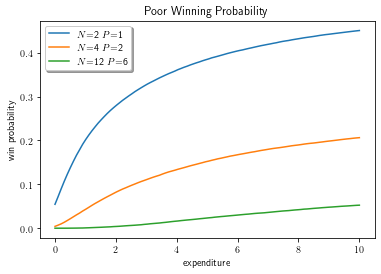
\includegraphics[width=5in]{subchapters/figures/poor_winning_probability_over_n_1_to_2}
\par\end{centering}
\caption{\label{fig:Probability-to-win-for-poor-with-N}Probability to win
for poor consumer with increasing number of participants}
\end{figure}

\begin{figure}
\begin{centering}
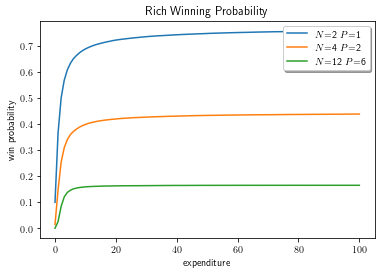
\includegraphics[width=5in]{subchapters/figures/rich_winning_probability_over_n_1_to_2}
\par\end{centering}
\caption{\label{fig:Probability-to-win-for-rich-with-N}Probability to win
for rich consumer with increasing number of participants}
\end{figure}


\subsection{\label{subsec:Two-player-Discrete-Model}Equilibrium Conditions}

\noindent

We proceed with a solution by setting total number of participants
$N=2$ and the number of poor participants $P=1$ in Equations \ref{eq:CaseI_general},
\ref{eq:CaseII_general} and \ref{eq:CaseIV_general} above. As before,
a participant takes advantage of the skills with weight $1-\mu$ only
by spending an amount $\overline{\nu}$ and can decide to avoid the
expenditure altogether in order to invest it towards the savings instead.
We first discuss the different probabilities in Case I, II, III and
IV before discussing the role of an additive intertemporal diminishing
utility from accumulated wealth. Recall that the behaviour of both
participants depends only on $\nu_{1},\nu_{2}$ - as they are unaware
of $r_{i},s_{i}$ before they participate. 

An important result for the closed-form solution is the probability
distribution (CDF) of $x_{i}\equiv\mu r_{i}+(1-\mu)s_{i}$ under assumption
$\mu<1-\mu$ (for independent variables $r_{i}$ and $s_{i}$ that
are uniformly distributed between 0 and 1) that is detailed in Appendix
\ref{sec:appendix_theorertical_1}.

\begin{align*}
F_{X}(x) & =P(x_{k}<x)=P(r_{k}\mu+s_{k}(1-\mu)<x)=\begin{cases}
\frac{x^{2}}{2\mu(1-\mu)} & 0<x<\mu\\
\frac{x-\mu/2}{1-\mu} & \mu<x<1-\mu\\
1-\frac{(x-1)^{2}}{2\mu(1-\mu)} & 1-\mu<x<1\\
0 & \text{otherwise}
\end{cases}
\end{align*}

We now evaluate above probabilities under Case I, II, III and IV discussed
above.

\subsubsection*{Case I}

In Case I, the poor participant can win when her raw-talent $r_{1}$
is higher than of the total score of rich participant (who competes
with acquired skills). The poor participant is priced out of accessing
any skills $s$ in her score so that the skills $s>0$ is only true
for the rich participant having $\nu_{2}$ $=\overline{\nu}$. Thus,
the poor participant with raw-talent $r_{1}$ can win with the following
probability

\begin{align*}
P(\text{win}|r_{1}) & =P(\mu r_{2}+(1-\mu)s_{2}<\mu r_{1})=F_{X}(\mu r_{1})
\end{align*}

Notice that $\mu r_{1}<\mu<1-\mu<1$ is implied due to $\mu<\frac{1}{2}$
(and $r_{1}\in(0,1)$ ). The probability that the total score $\mu r_{2}+(1-\mu)s_{2}$
does not exceed $\mu r_{1}$ implies that only the first part of the
piece-wise function for $F_{X}(x)$ needs to be considered. Therefore,
using $P(\text{win}|r_{1})=\frac{\mu^{2}r_{1}^{2}}{2\mu(1-\mu)}$,
we evaluate $P_{1}(\text{win})$ as 
\begin{align*}
P_{1}(\text{win})=\int_{0}^{1}P(\text{win}|r_{1})dr_{1} & =\frac{\mu}{6(1-\mu)}
\end{align*}
 

%integrate (mu^2*r^2,r,0,1)/(2*mu*(1-mu)) gives \frac{\mu}{6(1-\mu)}
% for .2, the probability is .03125. The MC gives .03126 . 

Since only one of the participants can win, the probability $P_{2}(\text{win})$
for the rich participant to win is simply $1-P_{1}(\text{win})$.
The following thus applies to all other cases (i.e. Cases II, III
and IV).

\begin{align}
P_{2}(\text{win}) & =1-P_{1}(\text{win})\label{eq:two_player_rich_probability}
\end{align}


\subsubsection*{Case II}

In Case II, the rich person does not participate ($\nu_{2}=0$) and
both the poor participants have the skills-advantage in the game.
A poor participant wins by having the total score higher than the
raw-talent of the rich participant (who does not acquire skills with
investment). Representing $x_{i}\equiv\mu r_{i}+(1-\mu)s_{i}$, we
have the following probability for the poor participant to win

\begin{align*}
P(\text{win}|r_{1},s_{1}) & =P(\mu r_{2}<\mu r_{1}+(1-\mu)s_{1})
\end{align*}

Notice that $P(\mu r_{2}<\mu r_{1}+(1-\mu)s_{1})$ (i.e. $P(r_{2}<r_{1}+(\frac{1}{\mu}-1)s_{1})$
) is $1$ after $r_{1}+(\frac{1}{\mu}-1)s_{1}>1$ ( or $\mu r_{1}+(1-\mu)s_{1}>\mu)$
and $\frac{1}{\mu}$ in the interval $(0,\mu)$ (this is because $r_{2}\in(0,1)$
). In other words, 

\begin{align*}
P(r_{2}<r_{1}+(1/\mu-1)s_{1}) & =\begin{cases}
\frac{x_{1}}{\mu} & 0<x_{1}<\mu\\
1 & \text{otherwise}
\end{cases}
\end{align*}

The probability to win for the poor participant can be written as
(see Appendix \ref{sec:appendix_theorertical_1})

\begin{align*}
P(\text{win}|r_{1},s_{1}) & =\begin{cases}
\frac{x_{1}}{\mu} & 0<x<\mu\\
1 & \mu<x_{1}<1-\mu\\
1 & 1-\mu<x_{1}<1\\
0 & \text{otherwise}
\end{cases}
\end{align*}

Using double-integral properties (see Appendix \ref{sec:appendix_theorertical_2}),
the total probability to win $P_{1}(\text{win})$ for a poor participant
is evaluated as follows

\begin{multline*}
P_{1}(\text{win})=\int_{s_{1}=0}^{s_{1}=1}\int_{r_{1}=0}^{r_{1}=1}P(\text{win}|r_{1},s_{1})ds_{1}dr_{1}=\int_{r_{1}=0}^{r_{1}=1}{\int_{s_{1}=0}^{s_{1}=\frac{\mu(1-r_{1})}{1-\mu}}\ \frac{(\mu r_{1}+(1-\mu)s_{1})}{\mu}ds_{1}dr_{1}}\\
+\int_{r_{1}=0}^{r_{1}=1}{\int_{s_{1}=\frac{\mu(1-r_{1})}{1-\mu}}^{s_{1}=1-\frac{\mu r_{1}}{1-\mu}}1\ ds_{1}dr_{1}}\\
+\int_{r_{1}=0}^{r_{1}=1}{\int_{s_{1}=1-\frac{\mu r_{1}}{1-\mu}}^{s_{1}=1}1\ ds_{1}dr_{1}}\\
=\frac{\mu}{3(1-\mu)}+\frac{1-2\mu}{1-\mu}+\frac{\mu}{2(1-\mu)}\\
=\frac{2\mu}{6(1-\mu)}+\frac{6(1-2\mu)}{6(1-\mu)}+\frac{3\mu}{6(1-\mu)}=\frac{6-7\mu}{6(1-\mu)}
\end{multline*}

The probability $P_{2}(\text{win})$ for the rich participant to win
follows from Equation \ref{eq:two_player_rich_probability}.

\subsubsection*{Case III }

In Case III, when neither the rich nor the poor participate in the
game, then the game depends only on raw-talents and both participants
have the same probability $\frac{1}{2}$ to win the game. This is
because $\int_{r_{i}=0}^{r_{i}=1}P(\text{win}|r_{i})dr_{i}=\frac{r_{i}^{2}}{2}|_{0}^{1}=\frac{1}{2}$.
Both the poor and rich participant have the same total probability
$\frac{1}{2}$ to win. 

\subsubsection*{Case IV}

In Case IV, when both rich and poor participants set $\nu_{1}=\nu_{2}=\overline{\nu}$,
then the poor participant can win only if her score $x_{i}$ is above
that of the rich participant. Therefore, 

\begin{multline*}
P(\text{win}|r_{1},s_{1})=P(\mu r_{2}+(1-\mu)s_{2}<\mu r_{1}+(1-\mu)s_{1})\\
=F_{X}(x_{1})
\end{multline*}

\begin{align*}
P(\text{win}|r_{1},s_{1}) & =\begin{cases}
\frac{x_{1}^{2}}{2\mu(1-\mu)} & 0<x_{1}<\mu\\
\frac{x_{1}-\mu/2}{1-\mu} & \mu<x_{1}<1-\mu\\
1-\frac{(x_{1}-1)^{2}}{2\mu(1-\mu)} & 1-\mu<x_{1}<1\\
0 & \text{otherwise}
\end{cases}
\end{align*}

While this integral can be evaluated based on symmetry arguments (
since $x_{i}$ is also randomly distributed), the integral $\int_{s_{1}=0}^{s_{1}=1}\int_{r_{1}=0}^{r_{1}=1}P(\text{win}|r_{1},s_{1})dr_{1}ds_{1}$
also evaluates to $\frac{1}{2}$ (see Appendix \ref{sec:appendix_theorertical_2})

\begin{multline*}
\int_{s=0}^{s=1}\int_{r=0}^{r=1}F_{X}(x_{1})ds_{1}dr_{1}=\int_{r_{1}=0}^{r_{1}=1}{\int_{s_{1}=0}^{s_{1}=\frac{\mu(1-r)}{1-\mu}}\frac{(\mu r_{1}+(1-\mu)s_{1})^{2}}{2\mu(1-\mu)}\ ds_{1}dr_{1}}\\
+\int_{r_{1}=0}^{r_{1}=1}{\int_{s_{1}=\frac{\mu(1-r)}{1-\mu}}^{s_{1}=1-\frac{\mu r}{1-\mu}}(\frac{\mu r_{1}+(1-\mu)s_{1}-\mu/2}{1-\mu})\ ds_{1}dr_{1}}\\
+\int_{r_{1}=0}^{r_{1}=1}{\int_{s_{1}=1-\frac{\mu r}{1-\mu}}^{s_{1}=1}(1-\frac{(\mu r_{1}+(1-\mu)s_{1}-1)^{2}}{2\mu(1-\mu)})\ ds_{1}dr_{1}}\\
=\frac{\mu^{2}}{8(1-\mu)^{2}}+\frac{1-2\mu}{2(1-\mu)}+\frac{(4-5\mu)\mu}{8(1-\mu)^{2}}=\frac{4(1-\mu)^{2}}{8(1-\mu)^{2}}=\frac{1}{2}
\end{multline*}

% For part A,  integrate( integrate((mu *r + (1-mu)*s)^2/(2*mu*(1-mu)),s,0,mu*(1-r)/(1-mu)) , r, 0,1) gives \frac{\mu^2}{8(1-\mu)^2}
% For part B, integrate (integrate( ((mu * r + (1-mu) *s - mu /2 )/(1-mu) ),s,mu*(1-r)/(1-mu),1-mu*r/( 1-mu)) , r, 0, 1)  gives \frac{1-2\mu}{2(1-\mu)}
% For part C, integrate(integrate( (1- ((mu *r  + (1-mu) * s)-1)^2/(2*mu*(1-mu))), s, 1-mu *r /(1-mu),1),r,0,1) gives \frac{(4-5\mu)\mu}{8(1-\mu)^{2}}
% simplified with  x^2 +(1-2*x)*(1-x)*4+(4-5*x)*x which gives 4(1-x)^2

\begin{figure}
\begin{centering}
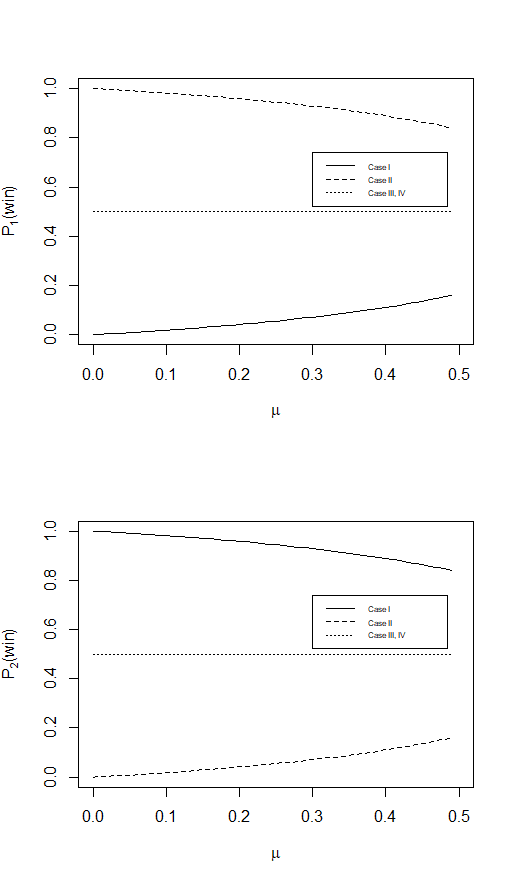
\includegraphics[width=4in]{subchapters/figures/winprob_with_mu_1_to_2}
\par\end{centering}
\caption{\label{fig:Probability-of-winning}Probability of winning $P_{1}(\text{win})$,
$P_{2}(\text{win})$ for poor and rich participants with varying $\mu$}
\end{figure}

As is clear from Figure \ref{fig:Probability-of-winning} and above
results (see summaries in Tables \ref{tab:Results_summary_poor} and
\ref{tab:Results_summary_rich}), the condition $\mu<1/2$ - indicating
that curated skills are given more importance that raw-talent in the
competitions - means that the poor participant is strictly better
off (than facing probability $1/2$) if she participates while the
rich participant doesn't participate (Case II). Also, the poor participant
is better off participating for $\mu<\frac{1}{2}$ when the rich participant
does participate as it raises the probability to $1/2$. That the
competition becomes uncompetitive both when threshold $\overline{\nu}$
falls too much (letting both participants participate) or rises too
much (letting both both participants withdraw) also follows from the
properties of the winning probability.

Notice that the rich participant could withdraw and face either $1/2$
or lower probability (when the poor participant participates). By
participating, therefore, the rich participant would either face probability
$1/2$ (when poor participant also participates) or better (if the
poor participant withdraws). Considering the probabilities alone,
the rich participant would always participate. If the rich participant
always participates, then so long as budget constraints permit, the
poor participant is also better off participating since not participating
brings her probability to win below $1/2$. If the utility was from
probability alone, then both participants would participate and face
$1/2$ probability.

However, it's not the probability to win that the participants are
likely to optimise (maximise). The participants are more likely to
face a finite life-time and utility from accumulated assets instead.
We therefore explore the case where the participants optimise an intertemporally
additive utility over their life-time. The life-time in the model
is represented with two time-horizons - where the second-time horizon
is one before the end of life when all wealth accumulated by either
participant must disappear. With no accumulations at the end of life,
both rich and poor participants must decide to spend all their incomes
$y_{1}$ or $y_{2}$ (for poor and rich participants respectively
so that $y_{1}<y_{2}$) towards the promotion game. In the first-stage,
however, the participants decide the amount to be spent towards promotion
based upon the utility from wealth they obtain across the two time-horizons
that span their lifetime. For the poor participant, the total utility
to be optimised (assuming EUT) under the intertemporally additive
utility $u(\cdot)$, a winning probability function $W(x)$ (for expenditure
$x$) and a discount-factor $\delta$ is 

\begin{align*}
u(y_{1}-\nu_{1})+\frac{1}{\delta}((1-W(y_{1}))u(y_{1})+W(y_{1})u(y_{2}))
\end{align*}

Similarly, for the rich participant, the total utility to be optimised
(assuming EUT) is 
\begin{align*}
u(y_{2}-\nu_{2})+\frac{1}{\delta}((1-W(y_{2}))u(y_{1})+W(y_{2})u(y_{2}))
\end{align*}

\begin{table}[H]
\begin{centering}
\begin{tabular}{>{\centering}p{0.7in}>{\centering}p{0.7in}>{\raggedright}m{1.5in}|>{\raggedright}m{1.5in}}
 &  & \multicolumn{1}{>{\raggedright}m{1.5in}}{Poor} & participant\tabularnewline
\begin{singlespace}
\end{singlespace}
 & \begin{singlespace}
\end{singlespace}
 & \begin{singlespace}
\textit{\small{}withdraws}
\end{singlespace}
 & \begin{singlespace}
\textit{\small{}participates}
\end{singlespace}
\tabularnewline
\begin{singlespace}
Rich
\end{singlespace}
 & \begin{singlespace}
\textit{\small{}withdraws}
\end{singlespace}
 & \multirow{1}{1.5in}{Case III} & Case II\tabularnewline
\cline{3-4} \cline{4-4} 
\begin{singlespace}
Participant
\end{singlespace}
 & \begin{singlespace}
\textit{\small{}participates}
\end{singlespace}
 & \begin{singlespace}
Case I
\end{singlespace}
 & \begin{singlespace}
Case IV
\end{singlespace}
\tabularnewline
\end{tabular}
\par\end{centering}
\caption{\label{tab:prisoners_dilemma_cases}Cases I,II, III, IV as participant
strategies}
\end{table}

\begin{table}[H]
\begin{raggedright}
{\footnotesize{}}%
\begin{tabular*}{1.2in}{@{\extracolsep{\fill}}>{\raggedright}p{0.5in}>{\raggedright}p{0.4in}>{\centering}m{2.5in}|>{\raggedright}m{2.2in}}
 &  & \multicolumn{1}{>{\centering}m{2.5in}}{\begin{onehalfspace}
{\footnotesize{}Poor}
\end{onehalfspace}
} & \begin{onehalfspace}
{\footnotesize{}participant}
\end{onehalfspace}
\tabularnewline
 &  & \begin{onehalfspace}
\textit{\footnotesize{}withdraws}
\end{onehalfspace}
 & \begin{onehalfspace}
\textit{\footnotesize{}participates}
\end{onehalfspace}
\tabularnewline
{\footnotesize{}Rich}\\
{\footnotesize{}participant} & \textit{\footnotesize{}withdraws} & {\footnotesize{}
\begin{gather*}
u(y_{2})+\frac{(1-\frac{P}{N})u(y_{2})+\frac{P}{N}u(y_{1})}{\delta}
\end{gather*}
}\\
{\footnotesize{}
\begin{gather*}
u(y_{1})+\frac{(1-\frac{P}{N})u(y_{2})+\frac{P}{N}u(y_{1})}{\delta}
\end{gather*}
} & {\footnotesize{}
\begin{gather*}
u(y_{2})+\frac{u(y_{2})p_{2}'+(1-p_{2}')u(y_{1})}{\delta}
\end{gather*}
}\\
{\footnotesize{}
\begin{gather*}
u(y_{1}-\overline{\nu})+\frac{u(y_{2})p_{1}'+(1-p_{1}')u(y_{1})}{\delta}
\end{gather*}
}\tabularnewline
\cline{2-4} \cline{3-4} \cline{4-4} 
 & \textit{\footnotesize{}participates} & {\footnotesize{}
\begin{gather*}
u(y_{2}-\overline{\nu})+\frac{p_{2}u(y_{2})+(1-p_{2})u(y_{1})}{\delta}
\end{gather*}
}\\
{\footnotesize{}
\begin{gather*}
u(y_{1})+\frac{p_{1}u(y_{2})+(1-p_{1})u(y_{1})}{\delta}
\end{gather*}
} & {\footnotesize{}
\begin{gather*}
u(y_{2}-\overline{\nu})+\frac{(1-\frac{P}{N})u(y_{2})+\frac{P}{N}u(y_{1})}{\delta}
\end{gather*}
 }\\
{\footnotesize{}
\begin{gather*}
u(y_{1}-\overline{\nu})+\frac{(1-\frac{P}{N})u(y_{2})+\frac{P}{N}u(y_{1})}{\delta}
\end{gather*}
}\tabularnewline
\end{tabular*}{\footnotesize\par}
\par\end{raggedright}
\caption{\label{tab:prisoners_dilemma}Utility from two periods for (rich,poor)
participants - at the start of the first-period (with $P$ poor participants
among $N$ total participants) }
\end{table}

\noindent

With above utilities, we discuss conditions for whether the Case I,
II, III, IV can become Nash equilibria (see Table \ref{tab:prisoners_dilemma_cases}).
We then proceed to discuss the implications for the effect of income
differences on expenditure towards status. It is worth remarking that
our discussion of the effect of the threshold $\overline{\nu}$ and
the income differences $y_{2}-y_{1}$ on participation (expenditure)
assumes that the exogenous parameter $\mu$ is stable with respect
to short-term changes in threshold investment $\overline{\nu}$ as
well as disposable incomes $y_{1},y_{2}$. 

For ease of notation we define $p_{1},p_{2},p_{1}'$ and $p_{2}'$
- which correspond to the\textbf{ two-player }model discussed above.

\begin{gather}
p_{1}\equiv\frac{\mu}{6(1-\mu)}\nonumber \\
p_{2}\equiv1-p_{1}\nonumber \\
p_{1}'\equiv\frac{6-7\mu}{6(1-\mu)}\label{eq:probabilities_2player}\\
p_{2}'\equiv1-p_{1}'\nonumber 
\end{gather}
 

The consumer choices for the poor and rich participants using a general
intertemporally additive function $u(A)$ (for assets $A$) are shown
in Table \ref{tab:prisoners_dilemma}. As we can verify from Figure
\ref{fig:Probability-of-winning} that we have $p_{1}<1/2<p_{2}$
and $p_{1}'>1/2>p_{2}'$ for all values of $\mu<1/2$.

\begin{gather}
\text{Given }\mu<1/2,\text{we have}\label{eq:probability_inequality}\\
p_{1}<1/2<p_{2}\nonumber \\
p_{1}'>1/2>p_{2}'\nonumber 
\end{gather}
 

Notice the Table \ref{tab:prisoners_dilemma} represents the condition
when the budget is non-binding i.e. the poor participant is able to
spend $\overline{\nu}$. i.e. $\overline{\nu}<y_{1}<y_{2}$. When
the poor participant faces a binding constraint i.e. $y_{1}<\overline{\nu}<y_{2}$
, then the rich participant knows that the best case probability to
win for the poor participant is $\frac{1}{2}$. The rich participant's
decision to participate would depend only on utility from savings
and the relative advantage from gain in probability. This is elaborated
further in Section \ref{subsec:Binding-constraint}.

Since the number of poor participants is likely to be higher than
that of rich participants in a typical competition, the unequal number
of poor and rich participants seems also worth considering in the
model. Setting $N=3,P=2$ in the equations \ref{eq:CaseI_general},
\ref{eq:CaseII_general} and \ref{eq:CaseIV_general}, for example,
we can interpret the \textbf{three-player} model with the following
values of $p_{1},p_{2},p_{1}'$ and $p_{2}'$ 

\begin{gather}
p_{1}=\frac{\mu}{8(1-\mu)}\nonumber \\
p_{2}=1-2p_{1}\nonumber \\
p_{1}'=\frac{19\mu^{2}-40\mu+20}{40(1-\mu)^{2}}\label{eq:probabilities_3player}\\
p_{2}'=1-2p_{1}'\nonumber 
\end{gather}

\begin{table}[H]
\begin{centering}
\begin{tabular}{|>{\centering}p{1cm}|>{\centering}p{3cm}|>{\centering}p{4cm}|>{\raggedright}p{7cm}|}
\hline 
Case & Description & Probability of poor participant to win & Response to $\mu$\tabularnewline
\hline 
\hline 
\begin{onehalfspace}
I
\end{onehalfspace}
 & \begin{onehalfspace}
Only rich invest in skills
\end{onehalfspace}
 & 
\begin{gather*}
\frac{\mu}{6(1-\mu)}
\end{gather*}
 & \begin{onehalfspace}
With higher $\mu$, the participants with raw-talent get rewarded.
The probability to win increases with higher $\mu$ for the poorer
participant.
\end{onehalfspace}
\tabularnewline
\hline 
\begin{onehalfspace}
II
\end{onehalfspace}
 & \begin{onehalfspace}
Only poor invest in skills
\end{onehalfspace}
 & 
\begin{gather*}
\frac{6-7\mu}{6(1-\mu)}
\end{gather*}
 & \begin{onehalfspace}
With higher $\mu$, the poor participants with access to skills get
rewarded. Therefore, The probability to win decreases with higher
$\mu$ for the poorer participant.
\end{onehalfspace}
\tabularnewline
\hline 
\begin{onehalfspace}
III,IV
\end{onehalfspace}
 & \begin{onehalfspace}
Neither or Both invest in skills
\end{onehalfspace}
 & 
\begin{gather*}
\frac{1}{2}
\end{gather*}
 & \begin{onehalfspace}
Probabilty to win is independent of $\mu$.
\end{onehalfspace}
\tabularnewline
\hline 
\end{tabular}
\par\end{centering}
\caption{\label{tab:Results_summary_poor}The probability of winning for the
poor participant in the 3-player model}
\end{table}

% Poor participant
% require(latex2exp)
% x = seq(0,.499,.01); plot(0,0,type='l',xlim=c(0,.5),ylim=c(0,1),xlab=TeX("$\\mu$"),ylab=TeX("P(win)")); 
% lines(x,(x*(x^2-2*x-3)+4)/(12*(1-x)),type='l',lty=1) # only rich
% lines(x,(-16*x**3 + 65*x**2 - 90*x + 40 )/( 120 * (1-x)**2),lty=2) # only poor
% lines(x,rep(1/3,length(x)),lty=3) # neither or both
% legend(0.3, .7,legend=TeX(paste("Case",c("I","II","III,IV"))),lty=c(1,2,3),cex=.7) 

\begin{table}[H]
\begin{centering}
\begin{tabular}{|>{\centering}p{1cm}|>{\centering}p{3cm}|>{\raggedright}m{4cm}|>{\raggedright}p{7cm}|}
\hline 
Case & Description & Probability of rich participant to win & Response to $\mu$\tabularnewline
\hline 
\hline 
\begin{onehalfspace}
I
\end{onehalfspace}
 & \multirow{1}{3cm}{\begin{onehalfspace}
Only rich \\
invest in skills
\end{onehalfspace}
} & \multirow{1}{4cm}{\begin{onehalfspace}
\begin{gather*}
1-\frac{\mu}{6(1-\mu)}
\end{gather*}
\end{onehalfspace}
} & \begin{onehalfspace}
With higher $\mu$, the participants with raw-talent get rewarded.
Therefore, the probability to win decreases with higher $\mu$ for
the rich participant.
\end{onehalfspace}
\tabularnewline
\hline 
\begin{onehalfspace}
II
\end{onehalfspace}
 & \begin{onehalfspace}
Only poor invest in skills
\end{onehalfspace}
 & \begin{onehalfspace}
\begin{gather*}
1-\frac{6-7\mu}{6(1-\mu)}
\end{gather*}
\end{onehalfspace}
 & \begin{onehalfspace}
With higher $\mu$, the poor participants with access to skills get
rewarded. Therefore, the probability to win increases with higher
$\mu$ for the rich participant.
\end{onehalfspace}
\tabularnewline
\hline 
\begin{onehalfspace}
III,IV
\end{onehalfspace}
 & \begin{onehalfspace}
Neither or Both invest in skills
\end{onehalfspace}
 & \begin{onehalfspace}
\begin{gather*}
\frac{1}{2}
\end{gather*}
\end{onehalfspace}
 & \begin{onehalfspace}
Probabilty to win is independent of $\mu$.
\end{onehalfspace}
\tabularnewline
\hline 
\end{tabular}
\par\end{centering}
\caption{\label{tab:Results_summary_rich}The probability of winning for the
rich participant in the 3-player model}
\end{table}

% Rich participant
% require(latex2exp)
% x = seq(0,.499,.01); plot(0,0,type='l',xlim=c(0,.5),ylim=c(0,1),xlab=TeX("$\\mu$"),ylab=TeX("P(win)")); 
% lines(x,1-(x*(x^2-2*x-3)+4)/(6*(1-x)),type='l',lty=1) # only rich
% lines(x,1-(-16*x**3 + 65*x**2 - 90*x + 40 )/( 60 * (1-x)**2),lty=2) # only poor
% lines(x,rep(1/3,length(x)),lty=3) # neither or both
% legend(0.3, .7,legend=TeX(paste("Case",c("I","II","III,IV"))),lty=c(1,2,3),cex=.7) 

Comparing these probabilities with those from the 2-player model in
Equation \ref{eq:probabilities_2player} (also listed in Tables \ref{tab:Results_summary_poor}
and \ref{tab:Results_summary_rich}), we see that the probability
to win for the poor participant in the 3-player model is lower with
respect to the Case III probability (i.e. $1/N$). Likewise, the probability
for the rich participant to win is higher in the 3-player model with
respect to the Case III probability ($1/N$). The implications for
the unequal number of poor and rich participants are further discussed
in Section \ref{subsec:Non-Binding-constraint}.

\begin{figure}
\begin{centering}
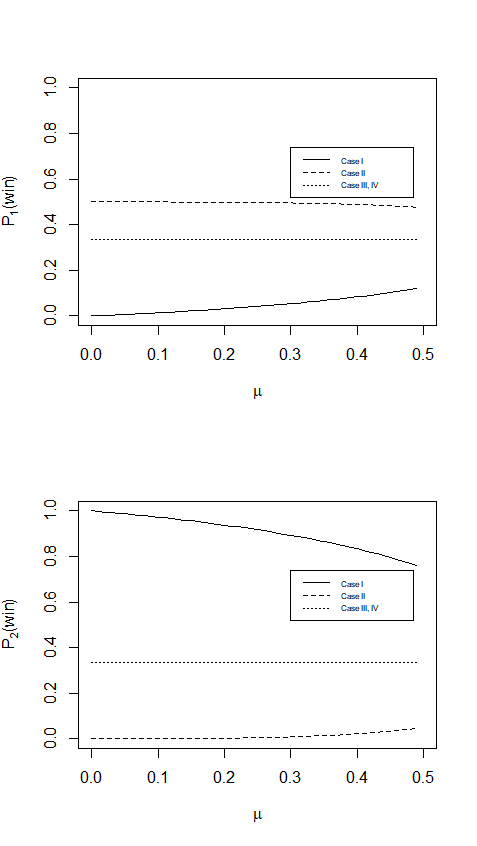
\includegraphics[width=4in]{subchapters/figures/winprob_with_mu_2_to_3}
\par\end{centering}
\caption{\label{fig:Probability-of-winning-2-to-3}Probability of winning $P_{1}(\text{win})$,
$P_{2}(\text{win})$ for poor and rich participants with varying $\mu$}
\end{figure}


\subsubsection{\label{subsec:Binding-constraint}Binding constraint}

\noindent

Assuming EUT participants we first consider the simpler case of binding
constraint $y_{1}<\overline{\nu}<y_{2}$. Since we assume a stability
in long-term participant behaviour (which itself is a result of observed
probability of success), mixed-strategies are not relevant in the
current set up. Considering pure strategies for participation, the
rich participant would thus participate only when the utility from
participating would be higher than from not participating i.e. $u(y_{2}-\overline{\nu})+\frac{p_{2}u(y_{2})+(1-p_{2})u(y_{1})}{\delta}>u(y_{2})+\frac{u(y_{2})+u(y_{1})}{2\delta}$
. This results in the following condition

\begin{align*}
\frac{(p_{2}-1/2)(u(y_{2})-u(y_{1}))}{\delta} & >u(y_{2})-u(y_{2}-\overline{\nu})
\end{align*}

With income differences being the same an increase in participation
cost $\overline{\nu}$ discourages participation since RHS increases
with $\overline{\nu}$ ($\because u(y_{2}-\overline{\nu})$ is decreasing
in $\overline{\nu}$) and may fail the above condition. Similarly,
with participation cost $\overline{\nu}$ being the same, an increase
in income-difference $y_{2}-y_{1}$ is in the rich participant's interest
whereas a narrowing of income differences reduces incentive for the
participant to participate by possibly failing the above condition.
All else being the same, higher impatience (lower time-discounted
value of money or a higher $\delta$) would also discourage participation.
Therefore, when budget is binding for the poor participant i.e. if
the poor participant cannot participate due to $y_{1}<\overline{\nu}$,
then narrower income differences, higher participation costs and higher
patience for savings (common for both rich and poor participants)
all encourage the rich participant to withdraw from the game. This
also means that wider income differences ($y_{2}-y_{1}$) combined
with lower participation costs ($\overline{\nu}$) may together help
maintain the equilibrium where only the rich participates. Similarly,
wider income differences ( higher $y_{2}-y_{1}$ ) and more patience
for savings (higher $\delta$) would together maintain the incentive
for the rich participant to participate. These conclusions very much
fit with the sociological observations made in the literature about
status \cite{HirschSocialLimits,GalbraithEssential}.

\subsubsection{\label{subsec:Non-Binding-constraint}Non-Binding constraint}

\noindent

When budget is non-binding, then participation of the rich participant
is her dominant strategy if the condition is also $u(y_{2})+\frac{u(y_{2})p_{2}'+(1-p_{2}')u(y_{1})}{\delta}<u(y_{2}-\overline{\nu})+\frac{u(y_{2})+u(y_{1})}{2\delta})$
i.e. 

\begin{align*}
\frac{(1/2-p_{2}')(u(y_{2})-u(y_{1}))}{\delta} & >u(y_{2})-u(y_{2}-\overline{\nu})
\end{align*}

The inferences on how $y_{2}-y_{1}$, $\overline{\nu}$ and $\delta$
influence the participation (see Section \ref{subsec:Binding-constraint})
remain the same for the above condition. To discuss the more general
Nash equilibria, we now consider the conditions for all of the Cases
I, II, III and IV to become a Nash equilibrium. For ease of notation
we define the following for a given $\overline{\nu},y_{1}$ and $y_{2}$

\begin{align*}
U_{1} & \equiv u(y_{1})-u(y_{1}-\overline{\nu})
\end{align*}

\begin{align*}
U_{2} & \equiv u(y_{2})-u(y_{2}-\overline{\nu})
\end{align*}

One could view $U_{1}$ and $U_{2}$ as the immediate gain in wealth
utility from withdrawing. If $u(\cdot)$ represents a diminishing
utility, then it is also necessary for $y_{1}<y_{2}$ that 

\begin{align*}
U_{2} & <U_{1}
\end{align*}

Consider now that conditions for Case I to be a Nash Equilibrium.
If Case I were to be a Nash equilibrium, then for the rich participant's
decision to participate, the poor participant must get more utility
from withdrawing than from participating and for poor participant's
decision to withdraw, the rich must get more utility from participating
than from withdrawing. The following conditions \footnote{$u(y_{1})+\frac{p_{1}u(y_{2})+(1-p_{1})u(y_{1})}{\delta}>u(y_{1}-\overline{\nu})+\frac{\frac{1}{N}u(y_{2})+\frac{1}{N}u(y_{1})}{\delta}\Rightarrow u(y_{1})-u(y_{1}-\overline{\nu})>\frac{(\frac{1}{N}-p_{1})(u(y_{2})-u(y_{1}))}{\delta}$
and $u(y_{2}-\overline{\nu})+\frac{p_{2}u(y_{2})+(1-p_{2})u(y_{1})}{\delta}>u(y_{2})+\frac{\frac{1}{N}u(y_{2})+\frac{1}{N}u(y_{1})}{\delta}\Rightarrow u(y_{2})-u(y_{2}-\overline{\nu})<\frac{(p_{2}-1/N)(u(y_{2})-u(y_{1}))}{\delta}$} must therefore hold simultaneously

\begin{gather}
\frac{(\frac{1}{N}-p_{1})(u(y_{2})-u(y_{1}))}{\delta}<U_{1}\nonumber \\
U_{2}<\frac{(p_{2}-1/N)(u(y_{2})-u(y_{1}))}{\delta}\label{eq:caseI_inequalities}
\end{gather}

% (\frac{(\frac{1}{3}-p_{1})(u(y_{2})-u(y_{1}))}{\delta},\frac{(p_{2}-1/3)(u(y_{2})-u(y_{1}))}{\delta})

Since $p_{2}-\frac{1}{N}\ge\frac{1}{N}-p_{1}$ (strict inequality
follows when the number of poor participants $P$ is higher than that
for rich participants $N-P$ e.g., with $N=3$ and $P=2$), this is
a fairly general condition for the equilibrium. An increase in $U_{1}$
due to higher $\overline{\nu}$ does not change the equilibrium conditions
so long as the corresponding rise $U_{2}$ (due to higher $\overline{\nu}$
) does not affect the second inequality. In other words, a higher
$\overline{\nu}$ favours the equilibrium (Case I) so long as there
is an incentive for the rich to participate. Likewise, a decrease
in $\overline{\nu}$ would be favourable for the equilibrium (Case
I) so long as the poor participants do not also have an incentive
to participate. 

Similar effects can be seen with income differences $y_{2}-y_{1}$
(which increase $u(y_{2})-u(y_{1})$ as well as $\frac{U_{2}}{U_{1}}$)
if we rewrite Equation \ref{eq:caseI_inequalities} as 

\begin{gather*}
\frac{(\frac{1}{N}-p_{1})}{\delta}<\frac{U_{1}}{u(y_{2})-u(y_{1})}\\
\frac{U_{2}}{(u(y_{2})-u(y_{1}))}<\frac{(p_{2}-1/N)}{\delta}
\end{gather*}

Limiting our attention to cases when $\overline{\nu}<y_{1}$, higher
$y_{2}$ for fixed $y_{1}$ decreases $\frac{U_{2}}{u(y_{2})-u(y_{1})}$and
makes it more likely for the rich to participate while it also decreases$\frac{U_{1}}{u(y_{2})-u(y_{1})}$
by raising the stakes enough for the poor to participate (making it
less likely for first inequality to be fulfilled). It is easy to see
that higher impatience $\delta$ encourages both poor and rich to
withdraw. As we shall see, equilibrium conditions corresponding to
Case II are far more stringent.

If Case II is a Nash Equilibrium, then for rich's decision to withdraw,
the poor participant should get more utility from participating than
from withdrawing and for poor participant's decision to participate,
the rich participant should get more utility from withdrawing than
from participating. This means that the following hold \footnote{$u(y_{1}-\overline{\nu})+\frac{p_{1}'u(y_{2})+(1-p_{1}')u(y_{1})}{\delta}>u(y_{1})+\frac{\frac{1}{N}u(y_{2})+\frac{1}{N}u(y_{1})}{\delta}\Rightarrow u(y_{1})-u(y_{1}-\overline{\nu})<\frac{(p_{1}'-1/N)(u(y_{2})-u(y_{1}))}{\delta}$
and $u(y_{2})+\frac{p_{2}'u(y_{2})+(1-p_{2}')u(y_{1})}{\delta}>u(y_{2}-\overline{\nu})+\frac{\frac{1}{N}u(y_{2})+\frac{1}{N}u(y_{1})}{\delta}\Rightarrow u(y_{2})-u(y_{2}-\overline{\nu})>\frac{(1/N-p_{2}')(u(y_{2})-u(y_{1}))}{\delta}$} simultaneously, 

\begin{gather*}
U_{1}<\frac{(p_{1}'-1/N)(u(y_{2})-u(y_{1}))}{\delta}\\
U_{2}>\frac{(1/N-p_{2}')(u(y_{2})-u(y_{1}))}{\delta}
\end{gather*}

Since $\frac{(p_{1}'-1/N)(u(y_{2})-u(y_{1}))}{\delta}<\frac{(1/N-p_{2}')(u(y_{2})-u(y_{1}))}{\delta}$
, the above cannot be satisfied so long as we have a diminishing utility
which necessitates $U_{2}<U_{1}$. Thus an equilibrium with Case II
which incentivises the poor to participate but not the rich is possible
only with a reference dependent utility with $U_{1}<U_{2}$. With
$U_{1}<U_{2}$, we can write above as 

\begin{gather*}
\frac{U_{1}}{u(y_{2})-u(y_{1})}<\frac{(p_{1}'-1/N)}{\delta}<\frac{(1/N-p_{2}')}{\delta}<\frac{U_{2}}{u(y_{2})-u(y_{1})}
\end{gather*}

Notice that despite a reference-dependent utility, a higher $\overline{\nu}$
or more impatience ($\delta$) may disincentivise the poor from participation
just the same (leading to Case III). Similarly, higher income differences
(an increase in $y_{2}$ for fixed $y_{1}$) could encourage the rich
to participate by decreasing $\frac{U_{2}}{u(y_{2})-u(y_{1})}$ (leading
to Case IV). Even with the reference dependent utility, the equilibrium
with Case II remains a fragile one.

If Case III were to be a Nash-Equilibrium, then for rich participant's
decision to withdraw, poor should get more utility from withdrawing
than from participating and for poor participant's decision to withdraw,
the rich participant should get more from withdrawing than from participating.
The following should thus hold\footnote{$u(y_{1})+\frac{\frac{1}{N}u(y_{2})+\frac{1}{N}u(y_{1})}{\delta}>u(y_{1}-\overline{\nu})+\frac{p_{1}'u(y_{2})+(1-p_{1}')u(y_{1})}{\delta}\Rightarrow u(y_{1})-u(y_{1}-\overline{\nu})>\frac{(p_{1}'-\frac{1}{N})(u(y_{2})-u(y_{1}))}{\delta}$
and $u(y_{2})+\frac{\frac{1}{N}u(y_{2})+\frac{1}{N}u(y_{1})}{\delta}>u(y_{2}-\overline{\nu})+\frac{p_{2}u(y_{2})+(1-p_{2})u(y_{1})}{\delta}\Rightarrow u(y_{2})-u(y_{2}-\overline{\nu})>\frac{(p_{2}-\frac{1}{N})(u(y_{2})-u(y_{1}))}{\delta}$},

\begin{gather*}
U_{1}>\frac{(p_{1}'-\frac{1}{N})(u(y_{2})-u(y_{1}))}{\delta}\\
U_{2}>\frac{(p_{2}-\frac{1}{N})(u(y_{2})-u(y_{1}))}{\delta}
\end{gather*}

Since $p_{1}'-\frac{1}{N}\le p_{2}-\frac{1}{N}$ (strict inequality
when number of poor participants is higher), we have $\frac{(p_{1}'-\frac{1}{N})(u(y_{2})-u(y_{1}))}{\delta}<\frac{(p_{2}-\frac{1}{N})(u(y_{2})-u(y_{1}))}{\delta}$
and $U_{2}<U_{1}$ . A higher $\overline{\nu}$ pushes both $U_{2}$
and $U_{1}$ further away from participation but a fall in $\overline{\nu}$,
incentivises the rich participant to participate (leading to Case
I). 

\begin{gather*}
\frac{U_{1}}{u(y_{2})-u(y_{1})}>\frac{(p_{1}'-\frac{1}{N})}{\delta}\\
\frac{U_{2}}{u(y_{2})-u(y_{1})}>\frac{(p_{2}-\frac{1}{N})}{\delta}
\end{gather*}

Higher income differences i.e. higher $y_{2}$ for fixed $y_{1}$
also decrease $\frac{U_{2}}{u(y_{2})-u(y_{1})}$ and incentivise the
rich participant to participate (leading to an equilibrium with Case
I). Conversely, if the game is not lucrative for the rich it would
automatically be infeasible for the poor i.e. if rich withdraws then
poor automatically withdraws. If there is any net utility from playing
the game, however, Case IV is the likely equilibrium.

If Case IV were to be a Nash Equilibrium, then for rich's decision
to participate, the poor participant should get more from participating
than from withdrawing and for poor's decision to participate, the
rich participant should get more from participating than from withdrawing.
Therefore, the following\footnote{$u(y_{1}-\overline{\nu})+\frac{\frac{1}{N}u(y_{2})+\frac{1}{N}u(y_{1})}{\delta}>u(y_{1})+\frac{p_{1}u(y_{2})+(1-p_{1})u(y_{1})}{\delta}\Rightarrow u(y_{1})-u(y_{1}-\overline{\nu})<\frac{(\frac{1}{N}-p_{1})(u(y_{2})-u(y_{1}))}{\delta}$
and $u(y_{2}-\overline{\nu})+\frac{\frac{1}{N}u(y_{2})+\frac{1}{N}u(y_{1})}{\delta}>u(y_{2})+\frac{p_{2}'u(y_{2})+(1-p_{2}')u(y_{1})}{\delta}\Rightarrow u(y_{2})-u(y_{2}-\overline{\nu})<\frac{(\frac{1}{N}-p_{2}')(u(y_{2})-u(y_{1}))}{\delta}$} must hold

\begin{gather*}
U_{1}<\frac{(\frac{1}{N}-p_{1})(u(y_{2})-u(y_{1}))}{\delta}\\
U_{2}<\frac{(\frac{1}{N}-p_{2}')(u(y_{2})-u(y_{1}))}{\delta}
\end{gather*}

With $\frac{(\frac{1}{N}-p_{2}')(u(y_{2})-u(y_{1}))}{\delta}<\frac{(\frac{1}{N}-p_{1})(u(y_{2})-u(y_{1}))}{\delta}$
and $U_{2}<U_{1}$ , this equilibrium rests upon the incentive for
the poor participant to participate. So long as the poorer participant
finds the competition worthwhile, the rich would also participate. 

The above results outline how participation costs influence the investments
towards status. For very low $\overline{\nu}$, rich and poor would
both participate and for very high $\overline{\nu}$, both would withdraw.
For everything in between, the only equilibrium with a diminishing
utility from wealth is one where rich participate whereas poor don't.

The above framework also allows us to discuss the implications of
inequality for the same total wealth in the economy. As such, a segregation
where the poor never participate in the status economy seems less
favourable than one where both rich and poor participate in the status
competitions. The current chapter explains that the likely outcome
of a failure to maintain universal participation in status games (under
diminishing utility from wealth) is that of a segregation where only
the rich participate in skills leading to economic success. While
a reference-based utility (which may be encouraged with segregation)
does seem to permit an equilibrium where only the poor are concerned
with status games (with respect to skills-enhancement), the result
only suggests that a segregation of status games along with that of
incomes is another possible long-term outcome of limited participation.

\section{\label{sec:Conclusion}Conclusion}

\noindent 

We have considered a model where status amounts to a position that
only temporarily cements the participant's economic position. With
a decision theory framework for uncertainty, the goal of the model
has been to investigate role of income difference on expenditures
that carry some status while also having some effect on the income
mobility of the participants. The endogenisation of status in this
manner allows us to use the framework to understand the role of income
difference in aspirational consumption under urbanisation effects
across economies that have varied status-determining cultural notions
as well as development indicators.

The foremost result from the model is that under diminishing utility
from wealth, the only two stable equilibria are those where both rich
and poor participate in status competitions and those where only rich
stand to benefit from status competitions. The model allows us to
understand how a withdrawal from expenditure such as education in
certain developing economies could be result of a combined effect
of both participation costs and income-differences. More specifically,
high participation costs push the equilibrium to one where where only
rich participate in status-related competitions whereas high income
differences may have the unlikely effect of incentivising the poor
consumers to participate. In the context of developing economies,
lowering of participation costs in education (as a status game) despite
rise in income differences may thus also represent a likely escape
from segregation of participation in the near-term for many developing
economies. The role of a reference-based utility adds an important
caveat to these results since contentment at lower levels of wealth
could support segregation of competitions at different income levels
in the economy.

\newpage

\section{Appendices}
\subsection{Convolution of Uniform Random Variables} \label{sec:appendix_theorertical_1}

The distribution of a convex combination $w=\mu r+(1-\mu)s$ of two
random variables $r,s$ - which are distributed according to densities
$f_{R}(r)$ and $f_{S}(s)$ - can be derived using the convolution
of two derived variables $x=\mu r$ and $y=(1-\mu)s$. If $r$ and
$s$ are uniformly distributed variables ranging from 0 to 1, then
$x$ ranges from 0 to $\mu$ and $y$ ranges from $0$ to $(1-\mu)$.
The CDF for $F_{X}(x)$ and $F_{Y}(y)$ are simply $F_{X}(x)=\frac{x}{\mu}$
, $F_{Y}(y)=\frac{y}{1-\mu}$ (respectively). Therefore, the densities
for $x$ and $y$ are $f_{X}(x)=\frac{1}{\mu}$ and $f_{Y}(y)=\frac{1}{1-\mu}$.
The density of $w$ is simple $f(w)=\int_{-\infty}^{\infty}f_{Y}(w-x)f_{X}(x)dx$.
Since , $f_{X}(x)$ is $1/\mu$ only between $0$ and $\mu$. We have
the following integral to evaluate for the convolution

\begin{align*}
f(w) & =\frac{1}{\mu}\int_{0}^{\mu}f_{Y}(w-x)dx
\end{align*}

Since $f_{Y}(y)$ is 1 only between 0 and $1-\mu$, we have the condition
$0<w-x<1-\mu\Rightarrow w-(1-\mu)<x<w$. Further, $x$ is distributed
only between 0 and $\mu$. As shown in Figure \ref{fig:convex_combo},
the integral would evaluate to the following\footnote{Notice that as a convex combination, $w$ is distributed only between
0 and 1.} under the assumption $\mu<\frac{1}{2}$.

\begin{align*}
f(w)=\frac{1}{\mu}\int_{0}^{\mu}f_{Y}(w-x)dx & =\begin{cases}
\frac{1}{\mu}\int_{0}^{w}\frac{1}{1-\mu}dx & 0<w<\mu\\
\frac{1}{\mu}\int_{0}^{\mu}\frac{1}{1-\mu}dx & \mu<w<1-\mu\\
\frac{1}{\mu}\int_{w-(1-\mu)}^{\mu}\frac{1}{1-\mu}dx & 1-\mu<w<1\\
0 & \text{otherwise}
\end{cases}
\end{align*}

This can be simplified as 

\begin{align*}
f(w) & =\begin{cases}
\frac{w}{\mu(1-\mu)} & 0<w<\mu\\
\frac{1}{1-\mu} & \mu<w<1-\mu\\
\frac{1-w}{\mu(1-\mu)} & 1-\mu<w<1\\
0 & \text{otherwise}
\end{cases}
\end{align*}

Figure \ref{fig:convex_combo_plot} shows this trapezoidal density
with $\mu$ set to $\frac{1}{5}$. The CDF $F_{X}(x)$ can be evaluated
by integrating the above density as $P(X<x)=\int_{-\infty}^{x}f(t)dt$. 

\begin{align*}
F_{X}(x) & =\begin{cases}
\frac{x^{2}}{2\mu(1-\mu)} & 0<x<\mu\\
\frac{\mu}{2(1-\mu)}+\frac{x-\mu}{1-\mu} & \mu<x<1-\mu\\
\frac{\mu^{2}}{2\mu(1-\mu)}+\frac{2\mu(1-2\mu)}{2\mu(1-\mu)}+\frac{\mu^{2}-x^{2}+2x-1}{2\mu(1-\mu)} & 1-\mu<x<1\\
0 & \text{otherwise}
\end{cases}
\end{align*}

Simplifying above, we have

\begin{align*}
F_{X}(x) & =\begin{cases}
\frac{x^{2}}{2\mu(1-\mu)} & 0<x<\mu\\
\frac{x-\mu/2}{1-\mu} & \mu<x<1-\mu\\
1-\frac{(x-1)^{2}}{2\mu(1-\mu)} & 1-\mu<x<1\\
0 & \text{otherwise}
\end{cases}
\end{align*}

\begin{figure}[H]
\begin{centering}
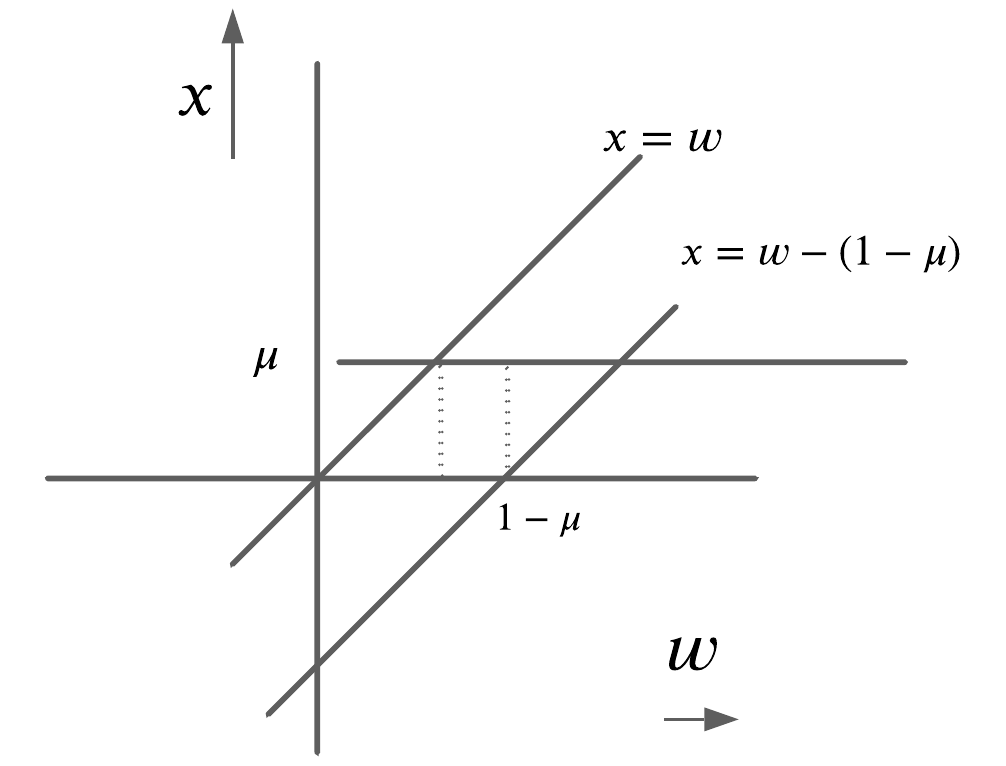
\includegraphics[width=4in]{subchapters/figures/combined_density}
\par\end{centering}
\caption{\label{fig:convex_combo}Ranges of $w$ and $w-x$ for convolution
of two scaled random variables}
\end{figure}

\begin{figure}[H]
\begin{centering}
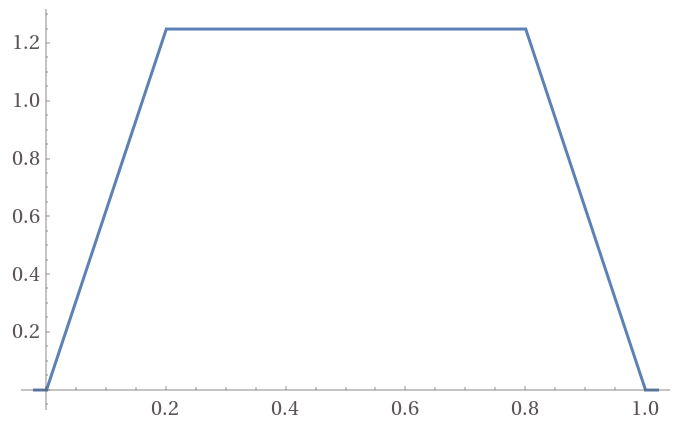
\includegraphics[width=4in]{subchapters/figures/combined_density_plot}
\par\end{centering}
\caption{\label{fig:convex_combo_plot}Combined density of $w$ as the convex
combination of two random variables with $\mu=\frac{1}{5}$}
\end{figure}

\newpage

\subsection{Double Integral of $P(\text{win}|r,s)$} \label{sec:appendix_theorertical_2} 

To calculate $\int_{s=0}^{s=1}\int_{r=0}^{r=1}P(\text{win}|r,s)drds$
over the variable $x$ (where $0<r<1$ and $0<s<1$), we evaluate
the sum of three parts split by the boundaries of the piecewise function.
The three parts are shown in Figure \ref{fig:integral_boundaries}.
If $x=\mu r+(1-\mu)s$ and $F(x)$ is of the following piece-wise
form

\begin{align*}
F(x) & =\begin{cases}
A & 0<x<\mu\\
B & \mu<x<1-\mu\\
C & 1-\mu<x<1\\
0 & \text{otherwise}
\end{cases}
\end{align*}

Then the integral $\int_{s=0}^{s=1}\int_{r=0}^{r=1}F(x)drds$ can
be written as

\begin{align*}
\int_{s=0}^{s=1}\int_{r=0}^{r=1}F(x)dsdr & =\int_{r=0}^{r=1}{\int_{s=0}^{s=\frac{\mu(1-r)}{1-\mu}}A\ dsdr}+\int_{r=0}^{r=1}{\int_{s=\frac{\mu(1-r)}{1-\mu}}^{s=1-\frac{\mu r}{1-\mu}}B\ dsdr}+\int_{r=0}^{r=1}{\int_{s=1-\frac{\mu r}{1-\mu}}^{s=1}C\ dsdr}
\end{align*}

\begin{figure}[h]
\begin{centering}
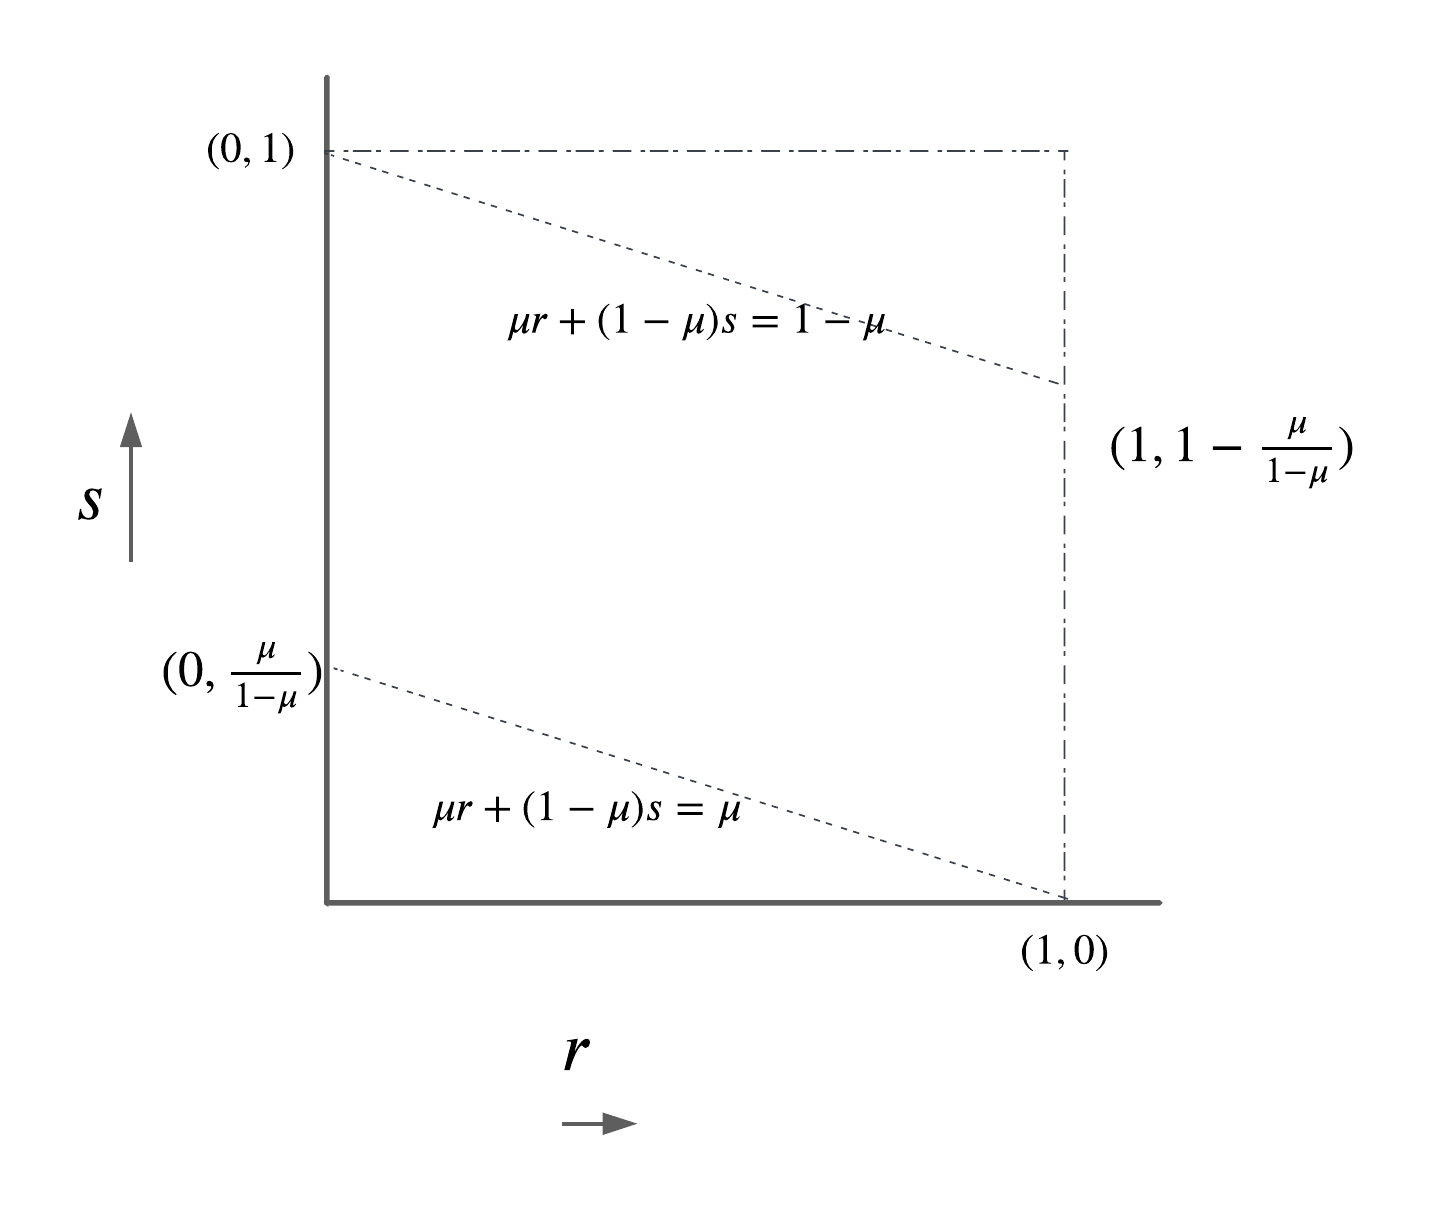
\includegraphics[width=4in]{subchapters/figures/integral_calculation}
\par\end{centering}
\caption{\label{fig:integral_boundaries}Integration over $r,s$ split by boundaries
$\mu r+(1-\mu)s=\mu$ and $\mu r+(1-\mu)s=1-\mu$}
\end{figure}

\newpage
\partfont{\fontsize{14}{16}\selectfont\centering} 

\part{\centering{Variation in Quality of Food Consumption in Tanzania}}

\vspace{2in}

\begin{abstract}
While consumption of basic needs may have hardly any status value
in societies where basic consumption needs have been fulfilled, food
continues to carry some status value in societies undergoing economic
transitions where it is either scarce or expensive. The presented
chapter explores the role of permanent income in demand substitution
for food quality in Tanzania where food continues to carry a status
significance. Comparing effects of permanent income and that of prices
of food commodities, we find a higher price-based quality associated
with meats and fruits to be aligned with the income disparities as
well as with the availability of electricity in Tanzania - suggesting
that the access to urban amenities also significantly differentiates
higher quality food consumption in the economy.
\end{abstract}
\onecolumn

\newpage

\section{Introduction}

\noindent

%## WHY QUALITY - Does a higher total expenditure imply a demand for better food quality in Tanzania? Notice that the research is about causes of aspirational consumption - not results of aspirational consumption.
% If snob didn't become bandwagon's the counterfeiting market would be absent.
% [barnett2005shoppingguccicanalst] - says emulation of snob is key. All else being the same, something that claims to emulate snobs would have more value. But why? Not merely because such a snob value is preferred by the consumers. If consumer go and act based on such values e.g., by entering subways and shops where they're likely to get noticed more easily or are preferred in interactions. There is some belief that being happier would make you more successful. It would because subjective wellbeing is not merely subjective it does seem to make you work harder and engage more with the economy (Why would you not engage more with the economy, if you feel that it's helping you become more like snobs). Barnett says that "several leading houses are believed to have undermined the reputation associated with a well-established brand by introducing a number of brand extensions and sub-product lines with lower quality than the original brand, by licensing logos and too widely, by failing to closely regulate retailers product displays and other sales practices, or simply by overproducing,so that firm's brand image became tarnished and sales ultimately fell.

While aspirational consumption is more often associated with extravagant
items of luxury, there seems strong evidence for aspirational items
becoming wider necessities in the population \cite{TimothyBurkeLifebuoyMen1996,barnett2005shoppingguccicanalst,silverstein2008tradingluxury,bekir2013luxurystrategy}.
As the access to high quality items expands to poorer sections of
the wider society, the notion of whether a certain item is aspirational
or not also changes with time \cite{barnett2005shoppingguccicanalst,silverstein2008tradingluxury,bekir2013luxurystrategy}.
In the context of sub-Saharan Africa (SSA), the current chapter examines
what demand for higher quality may imply for trends in aspirational
consumption. Using food as the basic need for this examination, the
chapter asks two particular questions that may help evaluate the expected
rise of high quality for basic needs in SSA \cite{SrivastavaMukherjee2020aspcon}.
First, it asks whether certain high-quality items stand out in food
consumption in a typical economy of sub-Saharan Africa (SSA) or not.
Second, it asks whether permanent income in urban as well as non-urban
areas significantly limits higher quality consumption for such items
of high quality. If the effects of permanent income on higher quality
are strong, then an overall rise in quality may largely depend on
how newer food items are introduced in urban and rural markets. The
chapter argues in favour of the conventional argument that a higher
quality being limited to richer sections of society puts evident limits
on the rise in consumption of such items \cite{HirschSocialLimits}.
To explore permanent income effects on high price-based quality, the
chapter employs a conventional quantity-based framework - while using
a dietary diversity standard to test whether certain items of higher
quality stand out in the survey of quality or not. It also tests whether
the quality consumed may be higher in more urbanised regions or not.

The analysis of food as an unlikely category of aspirational consumption
in the current chapter is motivated by two observations. First, there
seem compelling results from sociological surveys for status associated
with food in certain economies of SSA where a transformation from
agrarian to industrial societies is under way \cite{weismantel1989foodgenderpoverty,pottier1999anthropologyoffood,onuorah2003foodtaboos, ohna2007foodstatus}
. Second, a significant portion of household budget being spent on
food implies that the variation in food quality could detail the effects
of rising urbanisation on diets in a typical developing economy \cite{onuorah2003foodtaboos}.
A survey of variation in quality is of significance for studying sub-Saharan
African economies for other reasons as well. The strong preferences
that we observe in the current chapter towards certain items - preferences
which raise the overall food quality - are of interest from the perspective
of food policy due to the prevalent link between SES and poor dietary
diversity (DD) in the region \cite{HatloyFoodVarietySESMali2000,HoddinottDDFoodSec2002,RuelDDMethods2003, ArimondDDNutrition2004, StuntingAgriBio2017,HailuDDPregnantEthiopia2019,ModjadjiDDSA2020,   OBAYELUNigeriaDDLowIncome, AagadaIgbokweDDRuralNigeria2015,OgechiChilezieDDNigeria2017}.
A higher consumption of fruits and meats - which we find for urban
and richer households - also has implications for land use and environmental
concerns through increases in meat production and consumption.

%[OgechiChilezieDDNigeria2017, AagadaIgbokweDDRuralNigeria2015] starch or fatty foods)

While extreme variations in food quality and diet diversity are observed
many economies in SSA, the recent transition to urbanisation and compelling
results from sociological surveys in support of relevance of food
in status indication \cite{ohna2007foodstatus}present Tanzania as
an appropriate case-study for a study of variation in quality with
respect to inequalities. Other than the sociological studies of such
signaling value through food in both the pastoralist and agriculturalist
communities \cite{ohna2007foodstatus}, the recent experience of higher
consumption in Tanzania leaves wide disparities in asset ownership
and urbanisation levels - a disparity that allows us to understand
the role that variation in urban developments may play towards consumption
of basic needs. The ongoing urbanisation also leaves a significant
presence of semi-urban areas in Tanzania due in part to an incomplete
transition away from subsistence farming in the economy \cite{PiugaliSunderReviewNutritionDD2017,WenbanTNZFoodSecurityUrbanisation2016}
- a scenario that allows us to understand the permanent income effects
against urbanisation at a finer level of granularity.

A fundamental contention that we maintain for implications of permanent
income effects on food demand and rise in consumption is that higher
quality in any given food category may not be an instance of excessive
consumption. This is foremost because the notion of food-related basic
needs spans more than the minimal calorific intake required for survival
\cite{DoyalGoughNeeds1991}- allowing for consumption of quality at
the cost of its quantity for any particular food category to comprise
of basic necessities. Further, even if consumers are compelled to
increase quality in certain food categories rather than others (for
reasons unobserved), one needs a specific normative criteria to argue
that quality substitution of a particular food category with another
is actually excessive. Instead of determining whether the quality
consumed is excessive or not, our focus in the chapter remains on
assessing whether consumption of higher quality is narrowed down to
specific food categories relevant for food diversity or not and on
explaining what that may imply for consumption trends. While we do
use the FAO-specified nutrition categories \cite{KennedyBallardFantaFAO2011}
to help assess the extent to which higher quality in specific categories
may be aligned with recommended food diversity, the FAO-categories
are used only to provide a qualitative view of variation in quality
while avoiding any particular judgment on what is considered necessary
for the consumer. The empirical goal of the chapter is thus limited
to testing whether higher permanent income results in a higher demand
for quality across FAO-provided food categories in Tanzania or not.
The chapter discusses the implications for aspirational consumption
of factors other than permanent income - such as the role of availability
of basic amenities and urbanisation. It argues that while high quality
consumption may rise in future, a segregation of food demand based
on high or low permanent income may depend on how newer food items
are introduced in the market.

The analysis of variation in food quality relies on a robust framework
for quality in demand - where a measure for quality across commodities
(such as fruits, fat, meats-proteins etc.) upholds the theoretical
restrictions imposed by aggregation of demand across various goods
(such as coconut, mango etc. that may be classified within a commodity:fruits)
that are part of a commodity group (such as fruits). More specifically,
the method follows the restrictions implied due to the Hick's commodity
theorem \cite{Hicksvaluecapital1946,DeatonEconConsumer,NelsonQualityQuantity}
which requires the physical quantities of goods consumed to be weighted
by unchanging (relative) prices of the constituent goods before the
quantities can be aggregated into the demand for group whose quality
is measured. Thus, the quality of fruits as commodity - for example
- can be evaluated only as long as the goods - coconut, mango etc.
that may constitute the fruits commodity - exhibit a stable relative
price-structure. To avoid confusion in the terminology associated
goods and quality, we use the nomenclature provided by \citeA{CramerIncomePrice1973}
where ``goods'' or ``items'' are variants with different quality
that all fall under a certain ``commodity'' \cite{CoxWohlgenant1986}.

The particular theoretical approach is important for our analysis
of demand for quality due to two reasons. First, the approach is preferable
over an arbitrary aggregation of quality from groups that does not
follow the aggregation restrictions in a demand equation. Such restrictions
may limit our ability to talk about substitution in quality across
commodity groups - which is the core part of our assessment of how
quality availed of certain food categories may be higher than others.
Second, a robust aggregation based on market-prices also helps circumvent
measurement issues arising out of use of unit-prices \cite{GibsonKimQualityBog2019}.

The primary criterion of grouping the demand from goods consumed into
a commodity group using the approach is a stable relative price-structure
of market prices that are available in the consumption survey\footnote{The prices observed in local markets are those in the district where
the household - whose consumption is recorded for budget shares and
quality measures - is located.}. A classification of food items into commodities for which quality
metrics are calculated is thus undertaken using past observed-market
prices of all goods available in the survey alone - where a quality
metric is associated with each food commodity such that the constituent
goods of every commodity (which quality is calculated for) move together
in terms of their annual prices\footnote{A locally observed price associated with an item is one that is observed
for the item in the district where the household is located.} from 2008 to 2014. This is a departure from the unit-value approaches
where average expenditure itself is considered as a price-control.
It needs to be emphasised also that the groups of food-commodities
over which quality is evaluated are determined based on a similar
change in prices (rather than the prices themselves i.e. the classification
does not place all high-price items in one group and low-price groups
in another). The condition of a stable relative prices structure (due
to Hicks Commodity Theorem) drives a clustering of relative price
changes across all goods for food in the survey that we describe in
\ref{subsec:ClassificationGoods}. The FAO categories are then used
as the nutritional basis upon which we assess how the food demand
may have higher quality in certain commodity groups vs others. Thus,
the commodity groups obtained from the clustering are further divided
based on the twelve FAO (Food and Agriculture Organization of the
United Nations) categories - (i) cereals, (ii) vegetables, (iii) fruits,
(iv) meat, (v) eggs (vi) fish and other sea foods (vii) legumes, nuts
and seeds, (viii) milk and milk products (ix) oil and fats, (x) sweets
(xi) spices, condiments and beverages and (xii) tubers and roots \cite{KennedyBallardFantaFAO2011}
in order to provide a perspective from dietary diversity in quality.
The resultant commodities for which quality is evaluated are fat,
meats-proteins, cereals, vegetables, milk, starches, complements\footnote{Complements include miscellaneous items such as tea, sugar, coffee,
spices and salt - that are not considered in other categories.}, tubers, fruits, fish and chicken - steps that are further described
in Section \ref{subsec:ClassificationGoods}. The direct use of market-observed
prices also has the advantage that it avoids using unit-values (price-deflator)
as price controls in our analysis. More specifically, the market-prices
- used as controls in the analyses - avoid the measurement errors
that arise with the use of unit-values (which approximate the price
of an item with the average of item expenditure divided by its quantity
consumed). 

It is worth highlighting inferring qualities for commodity-groups
- based on an arbitrary or intuitive grouping criteria - may not follow
separability in demand or other restrictions of demand analysis either
\cite{DeatonEconConsumer}. As \citeA{NelsonQualityQuantity} points
out, an approach to consider a simple sum of quantities consumed from
across items (or goods) within a commodity group \cite{DeatonQualityQuantityVariation}
may only make sense if one imposes severe restrictions on consumer
preferences. The quality measure based on Hick's commodity theorem
that relies on market-observed prices remedies such issues without
imposing restricting assumptions on consumer demand \cite{Hicksvaluecapital1946,NelsonQualityQuantity}.
The measure also avoids intuitive grouping of goods into commodities
- thus avoiding the use researcher's own judgment of substitution
within commodity-groups.

Other than using the stable relative price-structure associated with
a commodity (fat, cereals etc.), the quality metric for every household
depends on the measurement of quantities of high vs low-price variants
(goods) consumed within a food commodity (e.g., the quantities consumed
of wheat, rice, maize for quality in cereals commodity). Considering
a commodity-group of cereals comprising of rice, maize and wheat,
for example, maize would contribute to lower quality of cereals-commodity
than wheat and rice if the prices (per-kg) of wheat and rice are higher
than that of maize. Other than the quality metric thus calculated
for every food commodity (such as cereals), the budget shares per
household for each of these commodities are used as dependent variables
in the system of equations used for an AIDS estimation. In order to
provide a comparison with a disaggregated view of goods consumed \cite{HeienWessellsAIDSCensored1990}
without any grouping into commodities, we also provide the results
from estimation of price elasticities for a disaggregated set of goods
consumed (see Appendix \ref{sec:appendix_food_2}).

The econometric method uses an AIDS formulation with both quality
metrics and budget shares as dependent variables \cite{DeatonMuellbauerAIDS}.
This is the ``Unrestricted Method'' AIDS formulation used by \cite{McKelveyQuality2011,AndalonGibsonSoda2017}
- with the total household expenditure - interpreted as permanent
income - as the main explanatory variable in the regression. The base-prices
- used as controls - are market prices directly observed in the survey
- rather than unit-prices which the empirical quality assessments
are often compelled to rely upon (despite issues with measurement
errors \cite{GibsonKimQualityBog2019}). The interpretation of household's
total expenditure as the permanent income measure in the study - is
common in the literature and relies on the standard consumption theory
(see \cite{modiglianiutility1954,FriedmanConsumption1957}). To highlight
the effect of wealth, we also present results from an alternative
formulation where the logarithm of reported value of total assets
owned by the households is used as the main explanatory variable.
The use of owned assets (land, house, furniture, vehicles, electronics
etc.) in wealth indices is also common in the health and consumption
studies \cite{HoweHargreavesWealthIndices2008,HoweHargreavesWealthIndexComparison2010,McKenzie2005,BooysenVanderbergAssetIndex2008}.

The results indicate that higher permanent income (measured as total
expenditure) is associated with higher demand for meat-related proteins
and fruits in particular. Further, the effect is made stronger due
to regional inequalities relating to variations in urbanisation levels
in Tanzania. More specifically, electricity being sparsely available
in the urban areas of Tanzania suggests strong effects of both electricity
availability and urbanisation levels on price-based quality (meats
and fruits in particular) \footnote{Since the prices of all items in the commodity move together, only
the base-price i.e. the minimum price in the commodity is used as
a control. This is detailed further Section \ref{tab:PriceBasedGroups}. }- despite controlling for permanent income (total expenditure). This
seems aligned with other studies on effects of resource availability
on food diversity in the region (see \cite{HailuDDPregnantEthiopia2019}
who explore the role of water availability on food diversity).

%[Contributions]

The presented chapter contributes to the literature in a few different
ways. First, it demonstrates that permanent income effects on quality
in a typical developing economy may not be uniform across food categories
nor across the income categories of consumers. This has implications
for how such consumption may rise with more economic growth and income
differences. Second, it investigates income effects on higher quality
using a more thorough as well as robust quality measure than the more
commonly used measures - such as the overall diversity measures or
intuitive item classifications. Third, it provides and employs a feasible
method to include food prices as controls in the discussion of regional
variation in quality without relying on detailed market prices of
every item.

In the sections that follow, the Section \ref{sec:LiteratureSurvey}
surveys the literature on quality of consumption, food diversity and
the relevance of often overlooked market prices in measurement of
quality. The approach to view quality across various commodities are
presented in Section \ref{sec:Model}. The details of the data used
in the study are provided in Section \ref{sec:Data} and a discussion
of the distribution of quality for food follows in Section \ref{sec:Results}.

\section{Literature Survey {\normalsize{}\label{sec:LiteratureSurvey}}}

\noindent

While consumption of basic needs (such as food) may have hardly any
status value in societies where the basic consumption needs have been
fulfilled \cite{HirschSocialLimits}, food continues to carry a status
value in societies where it is either scarce or signifies differences
in life-styles \cite{ohna2007foodstatus}. The differences among agricultural,
pastoral and urban life-styles in Tanzania that are reflected in food
habits present us an interesting case-study where differences in food
habits are indicative of one's social standing that are in turn influenced
by occupational status or regional belonging. 

As is often found in agrarian societies, the differences in food quality
as well as in the social values associated with the several variants
can be significant \cite{onuorah2003foodtaboos,ohna2007foodstatus}.
It is common in Tanzania, for example, that the guests are served
higher quality variants of commodities consumed by household. The
variation in social value can be significant even for variants that
are of similar nutritional value. In Tanzania, it is observed that
while the staple diet (\emph{ugali}) for many communities covers
a wide range spanning maize, \emph{kiwerege}, \emph{dona}, rice,
sorghum, cassava, millet and pumpkin, \emph{kiwerege} and rice invariably
carry more social value than millets or pumpkin \cite{ohna2007foodstatus}.
It is worth remarking that the different types of flour - varied only
by milling quality - tend to carry different social values. For example,
maize can be of \emph{kiwerege}, \emph{sembe} and \emph{dona} types
- out of which \emph{dona} is associated with poor communities and
\emph{kiwerege} carries the highest social value. This variation
seems even wider for non-staple food (\emph{mboga} ) which can be
used either as a side-dish or as a main meal (the latter being more
often for the pastoralist communities). While \emph{mboga} comprises
of beef, mutton, \emph{kuku} and other meats as well as beans, cabbage,
fermented milk and leafy-greens, meat carries more social value than
beans or cabbage. Further, meat and animal products are also used
as special foods during ceremonies and to treat the sick \cite{ohna2012nofoodwougali}.The
use of tomatoes, onion or red pepper invariably increase the social
status associated with the food served \cite{ohna2012nofoodwougali}.
The items of higher social value are invariably priced higher in the
consumer markets.

The effects of recent economic changes on food habits also seem evident
for communities in Tanzania - where an association with agriculture
seems to valued generally higher. For example, \emph{dona} is often
valued more among the pastoralist community than among agriculturalists\footnote{Some historical factors have also contributed to this variation such
as the past government distribution of sorghum leading it to be regarded
as of even lower social value than \emph{dona} among the agriculturalists. }. Urbanisation also seems to have brought particularly significant
changes in food habits as more food items have been introduced to
be consumed with between meals (with \emph{chai} or as \emph{kumbwa}
\cite{ohna2007foodstatus,ohna2012nofoodwougali}) - while a shift
away consumption of wild foods and meats is also under way \cite{ohna2007foodstatus}.
Given the status value of different varieties of food and the focus
on food in the LSMS data, a study of variation in food quality is
crucial to our exploration of high quality consumption for basic needs
in the context of aspirational consumption in Tanzania.

%From a nutritional science point of view, in the process of making kiwerege, essential nutrients are washed out of the maize flour.

The study of variation in food quality has had a long tradition in
empirical economics. One of the earliest approaches for measurement
of quality had been to treat it as a separate good \cite{HouthakkerQuality1952}
- thus decomposing the quality price elasticity of demand (quantity
purchased) into a quantity price elasticity of expenditure on quality
and an income elasticity of quality measure. The treatment of quality
as a separate good has been widely used ever since \citeA{DeatonEconConsumer}.
A common example of the approach is a simple repackaging method \cite{FisherShell1968}
- which interprets demand for a high-quality good as multiples of
lower quality goods. More specifically, the demand for goods with
a certain price using the repackaging approach is viewed in terms
of a base-price and a quality parameter - the implicit assumption
being that the variants in every category are perfect substitutes. 

For most empirical studies, however, the perfect substitution turns
out to be a stringent requirement since the variation in quality among
goods within a commodity may be often extreme. As an example, even
though quality consumed of electricity under energy commodity may
be higher than that of kerosene, the substitution between electricity
and kerosene may in fact be little - thus making it difficult to justify
a view of a demand for electricity in terms of the units of kerosene
consumed\footnote{While one may address this issue with use of an energy-budget (calories),
the unavailability of quantities consumed or prices in the consumption
data limit wider applications of such an approach.}. Nevertheless, simple-repackaging does turn out to be appropriate
in the context of cost-of-living index problems where a substitution
is implied \cite{FisherShell1968}.

%[Quality-Quantity metric details]

Some constraints on either consumer preferences or prices are needed
- when perfect substitution isn't possible - so as to measure the
quality using both quantities consumed and prices of goods within
a commodity. As such, the problem of measuring quality of a commodity
comprising of multiple goods is that of assigning a quality metric
to the entire commodity group using the a combination of quantities
consumed of the goods within the commodity group at prices known for
every good. As \citeA{NelsonQualityQuantity} explains, the approach
to measurement of food quality in such a manner must either assume
weakly separable preferences with homothetic within-group preferences
\cite{CoxWohlgenant1986,DeatonQualityQuantityVariation} or a stable
price-structure in a commodity group with a base-price associated
with the commodity. The current chapter opts for the latter approach
since it not only imposes fewer restrictions on the consumer preferences
but also makes use of the market prices rather than the unit-prices\footnote{The unit-prices are the total expenditure divided by quantities consumed
that are used prices as controls in a regression with budget, quantity
or quality as dependent variables.}. It is worth emphasising that the homotheticity of within-group preferences
presents\textbf{ }an implausible constraint on the demand - since
it implies either that the within-group income expansion path would
be a straight line through the origin or that the group composition
would remain independent of income - conditions. Such a restriction
on preferences would mean - for example - that the ratio of electricity
consumed to the kerosene consumed must be the same for both rich and
poor consumers - a constraint that is unlikely to hold empirically.

More formally, consider that in a generic sense, a quality-metric
associated with a certain commodity (e.g., cereals, fat etc.) depends
on a grouping of items - which the commodity comprises of - subject
to certain homogeneity restrictions. Given the quantity consumed $\{q_{i}\}_{i\in[1,n]}=\{q_{1},q_{2},...,q_{n}\}$
and respective prices $\{p_{i}\}_{i\in[1,n]}=\{p_{1},p_{2},...,p_{n}\}$
food $1\le i\le n$ goods, the quality-metric solves a problem equivalent
to the following disaggregated optimisation problem \cite{NelsonQualityQuantity}
for a direct utility $U(q_{1},q_{2},...)$ 

\begin{gather}
\max U(q_{1},q_{2},...q_{n})\nonumber \\
\sum_{i=1}^{n}p_{i}q_{i}=x\label{eq:disaggregated_problem}
\end{gather}

The quality metric problem is that of grouping the items $1\le i\le n$
into groups $1\le G\le M$ and assigning group-commodity price $P_{G}$
so that the solution of the problem in Equation \ref{eq:disaggregated_problem}
is equivalent to that of the problem in Equation \ref{eq:quality_groups_problem}

\begin{gather}
\max U(Q_{1},Q_{2},...Q_{M})\nonumber \\
\sum_{G=1}^{M}P_{G}Q_{G}=x\label{eq:quality_groups_problem}
\end{gather}

Such an aggregation requires that the $M$ groups (commodities) are
separable and that the demand for items within each group is a homogenous
function of the goods it contains \cite{NelsonQualityQuantity}. The
approach followed by \citeA{DeatonQualityQuantityVariation} - using
the sum of physical quantities as measure of demand - requires that
the homogeneity restriction is put on the household preferences while
assuming that the within-group preferences are homothetic. However,
the approach from \citeA{DeatonQualityQuantityVariation} (as well
as that from \citeA{CoxWohlgenant1986}) does not use the homogenous
commodities assumption and in fact permits heterogeneity in its use
of sums of physical quantities as the measure of demand \cite{NelsonQualityQuantity}.
The Hick's commodity theorem-based approach - which imposes a restriction
only on prices of goods - does not suffer with the issue as its use
in the current chapter does not impose the stringent homotheticity
assumption on preferences. 

Simply put, the approach we adopt in the current chapter prevents
considering chicken and eggs into one commodity unless the relative
price structure for the two items (chicken and eggs) does not change.
No other criteria - arbitrary or otherwise - is followed to group
the goods into commodities. Subject to the restriction, the notion
of quality is set to a price-weighted quantity (made possible due
the availability of market prices) so that given the same expenditure,
a lower quantity of the composite good (i.e. $Q_{G}$ for the composite
good $G$) corresponds to a higher quality and vice versa (see Section
\ref{sec:Model} for further details). The commodity groups thus selected
are obtained by clustering goods into commodity groups based on similar
price-changes over the years 2008, 2010, 2012 and 2014. A further
step sub-divides the clusters thus obtained based on the FAO provided
categories to assist interpretations from a DD perspective\footnote{The FAO provided categories are (i) cereals, (ii) vegetables, (iii)
fruits, (iv) meat, (v) eggs (vi) fish and other sea foods (vii) legumes,
nuts and seeds, (viii) milk and milk products (ix) oil and fats, (x)
sweets (xi) spices, condiments and beverages and (xii) tubers and
roots.}. 

The issue of unavailability of market prices - often sidelined in
many empirical studies - has recently gathered some attention \cite{McKelveyQuality2011,GibsonKimQualityBog2019}.
As such the measurement of quality is often performed without available
market prices - by simply averaging over the expenditures (recorded
costs) of a particular item in a given region (or over the entire
population of households). This so-called unit-value (or price-deflator)
method uses the average expenditure divided by quantity consumer for
all the consumers as prices in the empirical analyses (see \citeA{LazaridisMeatDemand2003,TafereTaffesseEthiopia2010}
for recent implementations). While using unit-values as prices may
be appropriate for certain empirical concerns, the measurement errors
introduced by their can be severe and difficult to ignore for finer
conclusions relating to price and income elasticities. More specifically,
the quantity consumed appearing both in the dependent variable (as
budget share's numerator) and in the control variable (as the denominator
for unit-value used as price) cannot be always mitigated \cite{McKelveyQuality2011,GibsonKimQualityBog2019}. 

The approaches such as the RDMP (``real'' deviations from regional/quarterly
mean prices) proposed by \citeA{CoxWohlgenant1986} that are implemented
without using locally observed market prices also suffer with the
same issue\footnote{For situations where market-prices are not available to such detail,
there have been a few techniques to address the measurement errors
arising from the use of price-deflators. \citeA{DeatonQualityQuantityVariation}
- for instance - uses cluster-average fitted budget shares and unit-values
in a cross-sectional analysis - an approach that has been elaborated
by \citeA{McKelveyQuality2011} for panel data analyses.}. The availability of detailed market-observed prices in the survey
- therefore not only helps with the fulfillment of Hick's Commodity
theorem through stable relative structure of prices - but also mitigates
the measurement errors that would be implied with the use of unit-values.

The econometric for the price-based quality metric uses the ``Unrestricted
Method'' for the AIDS model \cite{DeatonMuellbauerAIDS,AndalonGibsonSoda2017,GibsonKimQualityBog2019}.
Based on PIGL approaches originally popularised by \citeA{BartenPreferences},
\citeA{GormanPreference} and \citeA{MuellbauerAggConsum}, the AIDS
model readily conforms to the demand function restrictions and can
be extended for other panel data scenarios. For instance, the structural
changes in the parameters over time are addressed with a dynamic AIDS
formulation (see \citeA{AndersonBlundellDynEqn1982,AndersonBlundellAIDSTest1983}
for a first-order dynamic model) and the demographic variables are
accommodated using a ``demographic translation'' approach \cite{PollockWalesDemand}
. With prices $p_{j}$ for commodities $1\le j\le n$ , total expenditure
$x$, coefficients $\gamma_{ij}$ , $\beta_{i}$ for commodities $1\le i\le n$
and the price-index $P$, the demographic translation for the linear
AIDS formulation uses the following $\alpha_{i}$ intercept in AIDS
regression equation

\begin{align}
\alpha_{i} & =\rho_{io}+\sum_{k=1}^{s}\rho_{ik}d_{k}\label{eq:intercept_demographic_translation}
\end{align}

Specifically, the above intercept $\alpha_{i}$ for $1\le i\le n$
goods , $d_{k}$ are demographic variables and constants $\rho_{io}$
, $\rho_{ik}$ are used in the following AIDS regression where $w_{i}$
is the budget-share for the item $i$

\begin{align}
w_{i} & =\alpha_{i}+\sum_{j=1}^{n}\gamma_{ij}ln(p_{j})+\beta_{i}ln(\frac{x}{P})\label{eq:AIDS_linear}
\end{align}
 

Compared with the measurement of elasticities for every individual
good, the advantage with the aggregation over commodity groups is
that the latter does not present the issue of non-consumption of high-quality
goods. More specifically, if one were to calculate the price elasticities
for individual goods, an obvious issue that arises is that certain
items (particularly those with high-quality) might not be consumed
at all for a significant part of the population. \citeA{HeienWessellsAIDSCensored1990}
address this issue by correcting for non-consumption using the inverse
Mills ratio as instrument into the AIDS regressions. The Heien-Wells
(HW) approach effectively treats the consumption on high quality goods
``truncated'' for a significant part of the population\footnote{\citeA{HeienWessellsAIDSCensored1990} also use the unit-values instead
of (unavailable) market prices. Further, the unit-values obtained
from the households using a good are used as prices for those who
don't consume the good.}. While HW approach may be well-suited for comparison of elasticities
for specific goods (see Appendix \ref{sec:appendix_food_2} for empirical
results using the approach), the comparison of quality across multiple
commodities is a more appropriate interpretation for the overview
of quality we seek in the current chapter. Since it is much less likely
for no goods to be consumed within a broader commodity group (fruits-veg,
protein etc.) over which the quality measure is calculated, the approach
with quality aggregated over broader commodity groups also circumvents
the issue of non-consumption. No correction related to non-consumption
- as used in HW method - is therefore used with our approach that
aggregates quality over groups classified with homogeneity restrictions
(see Section \ref{subsec:ClassificationGoods}).

%[Nutrition and SES]

The variation in quality across multiple food sub-categories is examined
using the estimated income elasticities for quality using total household
expenditure as the main explanatory variable and urban-amenities as
key controls. While primarily exploring the role of food quality in
status, the current chapter also touches upon issues related with
SES effects on food diversity that have been remarked by many empirical
studies \cite{RuelDDMethods2003,HatloyFoodVarietySESMali2000}. In
particular, a lower within-country SES measure - whether it be in
developed or developing economies - often corresponds to less healthy
diets \cite{ManyangaTremblaySESDiets2017}. In a broad survey across
low and middle-income economies, \citeA{MayenSESDDlowmidIncomeCountries2014}
also find that with the exception of fruits in diet, the residents
of urban areas - particularly with higher SES - have more calorie
intakes as well as consumption of protein, fats and vitamins relative
to starchy items.

Some empirical studies also find a relevance of the availability of
amenities such as clean water on dietary diversity \cite{MekuriaWubnehDDFactorsEthiopia2017}.
A control for amenities such as electricity are also used - other
than total expenditure as our main explanatory variable - in the current
chapter to examine the variation in food quality across Tanzania.
In its particular context, rapid urbanisation seems to have brought
challenges to food security for the lower-income households in the
towns and cities within Tanzania - even though the country has managed
to maintain a broad self-sufficiency in basic food items \cite{WenbanTNZFoodSecurityUrbanisation2016}.
The agricultural policy has also focused on a transition from subsistence
farming to more efficient large-scale rural farming since urban farming
seems common in the country \cite{WenbanTNZFoodSecurityUrbanisation2016}.
As such, a significant number of households dependent on self-farming
in reportedly rural settings may obfuscate the relationship between
urban and rural food demand that may be apparent from the conventional
models for urban-rural migration \cite{HarrisTodaro1970}. The control
for urban-rural disparities is thus an important one for our survey
of food quality in the Tanzanian economy.

\section{Econometric Model\label{sec:Model}}

\noindent

The measure of quality used in the current chapter for each food commodity
group (such as fat, cereals etc.) comprising of multiple items (maize,
rice, wheat etc. for cereals etc.) relies on higher weights to high-priced
items (rice given higher weight than maize based solely on price etc.)
within each commodity group. The commodity groups over which the quality
is calculated are based on the price-structure restrictions implied
by the Hicks Commodity Theorem ( more details to follow in Section
\ref{subsec:ClassificationGoods}). A further sub-classification -
which does not disrupt the commodities identified based on similarity
of price structure - is used to assist interpretation from a DD perspective
and is guided by FAO categories recommended for food diversity. It
is worth highlighting that instead of measuring an overall food quality
across all of the food items consumed, we inspect quality only for
different commodity groups whose constituents satisfy the Hick's commodity
theorem. The quality across food can thus be seen as a vector associated
with the set of food commodities. As we detail in the Section \ref{subsec:ClassificationGoods},
the quality vector $\{V_{fat},$ $V_{meats-proteins}$, $V_{cereals}$
, $V_{vegetables}$,$V_{milk}$,$V_{starches}$, $V_{complements}$,$V_{tubers}$,$V_{fruits}$,$V_{fish}\}$
is based on price-correlation requirement from the Hicks Commodity
Theorem - while the groups based on movements are further subdivided
based on FAO categories to assist interpretations from a DD perspective. 

The data used for the classification as well as the inputs towards
estimation are described in Section \ref{sec:Data}.

\subsection{\label{subsec:ClassificationGoods}Classification in commodity groups }

% market_prices_2008 <- ll@load_market_prices(year = 2008, dirprefix = "../",fu = fu, ln=lsms_normalizer)
% market_prices_2010 <- ll@load_market_prices(year = 2010, dirprefix = "../",fu = fu, ln=lsms_normalizer)
% market_prices_2012 <- ll@load_market_prices(year = 2012, dirprefix = "../",fu = fu, ln=lsms_normalizer)
% market_prices_2014 <- ll@load_market_prices(year = 2014, dirprefix = "../",fu = fu, ln=lsms_normalizer)
% market_prices_national2008 <- ddply(market_prices_2008,.(shortname),summarise,price=median(median_price))
% market_prices_national2010 <- ddply(market_prices_2010,.(shortname),summarise,price=median(median_price))
% market_prices_national2012 <- ddply(market_prices_2012,.(shortname),summarise,price=median(median_price))
% market_prices_national2014 <- ddply(market_prices_2014,.(shortname),summarise,price=median(median_price))
%f1=fu()@rbind_xy(x = market_prices_national2008,y = market_prices_national2010, tagx=2008, tagy=2010)   
% f2=fu()@rbind_xy(x = f1,y = market_prices_national2012, tagy=2012)   
%f3=fu()@rbind_xy(x = f2,y = market_prices_national2014, tagy=2014)   
% 

\noindent

The main criterion of grouping of food items into commodity groups
is the co-movement of prices. The prices - shown in Figure \ref{fig:LSMSMarketPrices}
- are taken from the wave corresponding to years 2008, 2010, 2012
and 2014 in the survey. An unsupervised k-means clustering is then
used to group the items into commodities based on price changes -
so that the items within every commodity group identified have ``similar''
relative price-changes. The groups based strictly on price-movements
thus obtained are then split into further categories aligned with
the FAO recommended categories i.e. (i) cereals, (ii) vegetables,
(iii) fruits, (iv) meat, (v) eggs (vi) fish and other sea foods (vii)
legumes, nuts and seeds, (viii) milk and milk products (ix) oil and
fats, (x) sweets (xi) spices, condiments and beverages and (xii) tubers
and roots. More specifically, the k-means clustering is performed
on the relative price-changes from available prices. Considering beef
as an example good, the prices for beef in the years 2008, 2010, 2012,
2014 (see Figure \ref{fig:LSMSMarketPrices}) are $p_{beef}=\{3500.0,4000.0,5000.0,6000.0\}$
- which correspond to a relative price-change vector $r_{beef}=\{\frac{4000}{3500},\frac{5000}{4000},\frac{6000}{5000}\}=\{1.14,1.25,1.2\}$.
The relative price-change vectors for all the items (beef, goat, fresh\_milk
etc.) thus obtained are clustered using the k-means method - where
the number of selected clusters is guided by the within-cluster sum
of squared errors - an approach commonly used in k-means applications
\cite{Pollard1982CLTKmeans}. The classification we use as the basis
for commodity groups are arrived at by setting the number of clusters
to 5 which is when the within-cluster sum of squared errors drops
to less than unity\footnote{A higher number of clusters does not significantly reduce the within-cluster
sum of squared error.}. The classification of items based on these FAO-categories and the
correlated-price-movement is presented in Table \ref{tab:GroupsModified}.

It is worth emphasising that the partition of commodity groups identified
from the unsupervised k-means clustering into further sub-groups based
on FAO categories does not pick goods from disparate clusters into
a new sub-group. Instead, the further partition into sub-groups based
on FAO categories is based on the observation that that the price-changes
of goods within sub-groups formed by splitting a particular group
identified by clustering would also be correlated with each other.
The groups obtained by the classification based on correlation prices
(shown in Table \ref{tab:PriceBasedGroups}) are thus split into further
sub-groups aligned with the FAO groups in Table \ref{tab:GroupsModified}.
More specifically, the commodity cereals-milk-greens is split into
milk, veg and cereals, fruits-fish is split into fruits and fish,
startches-fats-complements is split into starches, fats and complements
while the categories tubers and meatsproteins are retained. The resulting
categories are therefore i) cereals ii) veg iii) fruits iv) meats-proteins
v) fish vi) milk vii)fat viii) complements ix) tubers x) chicken and
xi) starches whose constituents are shown in Table \ref{tab:GroupsModified}. 

\begin{table}
\begin{centering}
\begin{tabular}{|>{\raggedright}p{3cm}|>{\raggedright}p{7cm}|}
\hline 
food group & \multirow{1}{7cm}{food items}\tabularnewline
\hline 
\hline 
fat & cooking\_oil, eggs\tabularnewline
\hline 
meats-proteins & beef, goat, pork, pulses, onion, salt, canned\_milk, wild\_birds,
wild\_meat\tabularnewline
\hline 
cereals & rice\_husked, maize\_green, maize\_grain , wheat, maize\_flour\tabularnewline
\hline 
vegetables & greens, othervegstarch\tabularnewline
\hline 
milk & fresh\_milk, milk\_products\tabularnewline
\hline 
starches & sugarcane, millet\_grain, rice\_paddy, potatoes, canned\_drink, sweet\_potato,
bread\tabularnewline
\hline 
chicken & chicken\tabularnewline
\hline 
complements & sugar, tea, coffee, sweet, miscdrinkpowder, readymade\_tea\_coffee,
honey, spices\tabularnewline
\hline 
tubers & yam, millet\_flour, banana\_green, cassava\_flour\tabularnewline
\hline 
fruits & banana\_ripe, cassava\_fresh, peanuts, citrus, coconut, cashew\_almonds,dried\_canned\_veg,
nut\_products, mangoes\tabularnewline
\hline 
fish & dried\_canned\_fish, fish\_seafood, packaged\_fish\tabularnewline
\hline 
\end{tabular}
\par\end{centering}
\caption{\label{tab:GroupsModified}Food items classified into commodity groups
after considering both price-movements and FAO categories}
\end{table}

\begin{table}
\begin{centering}
\begin{tabular}{|>{\raggedright}p{2.2cm}|>{\raggedright}p{7cm}|}
\hline 
food group & \multirow{1}{7cm}{food items}\tabularnewline
\hline 
\hline 
meats-proteins & beef, goat, pork, pulses, onion, salt canned\_milk, wild\_birds, wild\_meat\tabularnewline
\hline 
cereals-milk-greens & rice\_husked, greens , othervegstarch, maize\_green, maize\_grain
, wheat, maize\_flour , fresh\_milk, milk\_products\tabularnewline
\hline 
starches-fats-complements & cooking\_oil, eggs, sugar, tea, sweet, sugarcane, coffee, chicken,
bread, potatoes, sweet\_potato, canned\_drink, miscdrinkpowder, readymade\_tea\_coffee,
honey, spices, millet\_grain, rice\_paddy\tabularnewline
\hline 
tubers & cassava\_flour, yam, millet\_flour, banana\_green,\tabularnewline
\hline 
fruits-fish & banana\_ripe, cassava\_fresh, peanuts, citrus, coconut, mangoes, dried\_canned\_veg,
dried\_canned\_fish, cashew\_almonds, nut\_products, fish\_seafood\tabularnewline
\hline 
\end{tabular}
\par\end{centering}
\caption{\label{tab:PriceBasedGroups}Food items classified into commodity
groups based on price-movements (without splitting into FAO-based
categories)}
\end{table}

As explained before, the basis for the quality metric associated for
every commodity $G$ (corresponding to the left side of the Table
\ref{tab:GroupsModified}) is the Hick's commodity theorem \cite{Hicksvaluecapital1946}
which states that a group of goods behave as if they were a single
commodity so long as the prices of the group of goods changes in the
same proportion. Simply put, a constant relative price structure allows
us to factor out the quantity of the composite commodity consumed
from the demand function for the variants (goods) within the commodity
- allowing the price of quality to be interpreted in terms of a composite
price $P_{G}$ for the commodity aggregate $G$ and the price-structure
$p_{G}^{*}$ from $n$ goods with prices $p_{G}=\{p_{i,G}\}_{i\in[1,n]}$.
With $E_{G}$ as the total expenditure on group $G$, the constant
relative price-structure permits us to write the commodity-aggregate
specific demand function $g(E_{G},p_{G})$ in terms of the price-structure
$p_{G}^{*}$ as follows

\begin{alignat}{1}
g(E_{G},p_{G}) & \equiv g(\frac{E_{G}}{P_{G}},p_{G}^{*})=g(Q_{G},p_{G}^{*})\label{eq:demand_function_quality}
\end{alignat}

The formulation in Equation \ref{eq:demand_function_quality} depends
both on the quantity $Q_{G}\equiv\frac{E_{G}}{P_{G}}$ and a quality
variable $V_{G}$\footnote{The income elasticity of composite quantity $Q_{G}$ is the sum of
income elasticity of quality $V_{G}$ and the income elasticity of
physical quantity $q_{G}$. This is further explained in Section \ref{subsec:QualityMeasure}
(see \cite{NelsonQualityQuantity} for more details). }. The essential appeal of aggregation is the simplified view of demand
across all items. Consider for example, if we were to represent demands
for items \{wheat, rice, yam,coconut, eggs, beef, chicken, fish, goat,
honey\}. As such these items would each correspond to a demand function
so that 10 functions describe the demand for all the 10 items. The
aggregated view allows us to view demands for commodities \{carb,
protein and complements\} - where the 10 goods are encompassed in
just 3 respective functions for the 3 commodity groups. A key requirement
for the validity of such a quality metric - however - is that the
prices of goods within the commodity group have a constant relative
price-structure i.e. a relative prices ratio that can be factored
out of the observed prices (see \cite{DeatonQualityQuantityVariation,NelsonQualityQuantity,GibsonKimQualityBog2019}).
This condition - due to the Hicks commodity theorem - drives the k-means
grouping of items described above.

In summary, the commodity aggregates used in the study are based on
a \textit{price-movement} sense (based on the Hick's commodity theorem)
- while a further splitting of groups is guided by a \textit{functional}
sense implied by FAO categories. Every commodity aggregate on the
left side of Table \ref{tab:GroupsModified} has goods with a similar
price-movement \textit{and }the same functional significance while
every commodity aggregate $G$ on the left side of Table \ref{tab:PriceBasedGroups}
has items that have only a similar price-movement\footnote{A similar analysis of rice varieties is conducted by \cite{McKelveyQuality2011}
.} . To explain with particular example goods, consider two pairs of
items with similar price-movements - with sugar and tea being the
first pair that have similar price changes (see Table \ref{tab:PriceBasedGroups}).
Let the second pair be rice and cooking-oil - who also have price
changes similar to each other (see Table \ref{tab:PriceBasedGroups}).
Notice however that not only do sugar and tea have similar price changes,
they also have a similar functional sense implied by FAO categories.
Therefore, they are classified in a group \textit{complements} in
the Table \ref{tab:GroupsModified}. Rice and cooking-oil on the other
hand are split into two categories based on the different functional
sense implied by FAO-categories (see Table \ref{tab:GroupsModified}).
Other categories such as meatsproteins, fruits etc. are similarly
based foremost on price-movement correlations before considering the
functional sense implied by FAO categories for interpretation from
a DD perspective.

\subsection{\label{subsec:QualityMeasure}Price-based quality}

\noindent

The vector of quality for every household comprises of the quality
$\nu_{G\in\mathscr{G}}$ associated with the commodity group $G\in\mathscr{G}$
where $\mathscr{G}$ is the set of all commodities relevant for the
household $\mathscr{G}$$=$$\{cereals$, $veg$, $fruits$ , $meats\_proteins$,
$fish$ , $milk$, $fat$, $complements$, $tubers$, $starches$\}.
Based on the local market-observed prices of the goods within the
commodity group $G\in\mathscr{G}$ (such as cereals, fat etc.), the
quality metric for the household ensures that a household who buys
more of the high-priced good within a commodity group is viewed as
one consuming higher quality of the commodity $G$. This is why no
quality is considered for chicken, the only good within its own commodity
group. As we've explained in Section \ref{subsec:ClassificationGoods},
the k-means clustering interprets the restriction that there is a
constant relative price structure on the constituent items of commodity
group (the Hicks aggregation condition).

To calculate the quality associated with a group $G\in\mathscr{G}$
(such as the items : beet and goat in the commodity: meatsproteins)
that have a constant within-group relative price-structure, a base-price
$P_{G}$ for the group $G$ (meatsproteins) is selected as the minimum
price of the items among the commodity aggregate constituents (e.g.,
among beef and goat). This is based on the approach suggested by \cite{NelsonQualityQuantity}.
The base-price $P_{G}$ is then used to assign i) an aggregate-quantity
of a composite good (for meatsproteins) comprising of quantities consumed
of the items constituted in $G$ (beef, goat) and ii) a quality metric
corresponding to $G$ ( based on the proportion of goat and beef consumed).
In other words, with the quantities consumed for beef and goat under
meatsproteins commodity available to us, a quantity of ``meatsproteins''
is associated with the particular set of quantities consumed for beef
and goat. The aggregate-quantity of ``meatsproteins'' is then calculated
by relative-prices-weighed averages of beef and goat consumed (see
details below). If beef per unit-weight is cheaper than goat-per-unit-weight,
then this quality metric would evidently be lower when more beef is
consumed for the same expenditure. This notion of higher-quality is
thus based solely on price alone so that a more expensive item within
the commodity group contribute to higher quality of the commodity.

In more formal terms, quantity-price tuples $(q_{1},p_{1}),(q_{2},p_{2}),(q_{3},p_{3})...$
within a commodity thus correspond to a quantity and quality pair
$(Q_{G},P_{G})$ as well as a quality metric $V_{G}$. We define the
total physical sum of quantities consumed $q_{G}$ as follows

\begin{align*}
q_{G} & =\sum_{j\in G}q_{j,G}
\end{align*}
 

Further, with $p_{i,G}$ as the prices for good $i$ in commodity
group $G$ observed in the market, we represent the price-structure
ratios for the good $i$ in a group $G$ as $p_{i,G}^{*}$ . The ratio
$p_{i,G}^{*}$ is effectively a price-multiple with respect to the
base-price $P_{G}$ (the price of the base-commodity in the group
$G$ with respect to which the quality in $G$ is being considered)
so that the observed prices $p_{i,G}$ of the items within the group
$G$ bear the following relationship:

\begin{alignat}{1}
p_{i,G} & =(P_{G}\times p_{i,G}^{*})\forall i\in G\label{eq:base_price_structure}
\end{alignat}

The quality metric $V_{G}$ then corresponds to the a sum of quantities
consumed $q_{i,G}$ weighted by the price-structure ($p_{i,G}^{*})$
for the commodity aggregate $G$ as follows

\begin{alignat}{1}
V_{G} & =\sum_{i\in G}(\frac{q_{i,G}p_{i,G}^{*}}{q_{G}})\label{eq:quality_def}
\end{alignat}

Following \cite{NelsonQualityQuantity}, we reject the use of sum
of physical quantities $q_{G}=\sum_{i\in G}q_{i}$ itself as $Q_{G}$
(as used by \cite{DeatonQualityQuantityVariation} - see Equations
\ref{eq:quality_groups_problem} and \ref{eq:demand_function_quality})
in favour of the above relative-price-weighted sum of expenditure
per physical unit (within the commodity $G$)\footnote{\cite{NelsonQualityQuantity} argues that the composite good quantity
$Q_{G}$ can be equivalent to the sum of physical quantities $q_{G}$
(i.e. $Q_{G}=q_{G}$ ) only if the quality effects are absent. With
$U_{G}=\frac{E_{G}}{q_{G}}$ as the unit quantity consumed this is
implied due to $Q_{G}=q_{G}\Rightarrow\frac{E_{G}}{P_{G}}=\frac{E_{G}}{U_{G}}\Rightarrow P_{G}=U_{G}$
. }. 

Let's consider an example to illustrate how the measure of quality
would relate with the total expenditure $E_{G}$ in the group $G$
and the group aggregate price $P_{G}$ (see \cite{NelsonQualityQuantity}
for a more detailed theoretical discussion). Let's say we observe
the consumption on goat and beef within a meatsproteins commodity
with prices observed as 20�, 10� (resp.) and the quantities consumed
by the household are 1.5 kg and 2 kg (resp.). One approach is to the
treat the physical sum of quantities i.e. 3.5 kg as the quantity of
the composite good ``meatsproteins''. However, it is more difficult
to argue that the households optimise the weight of the composite
good - rather than comparing the disparate quantities of goods (see
\cite{NelsonQualityQuantity} for details of this argument). Since
quality is to be priced in the market, a quality-adjusted quantity
is the more appropriate formulation where we consider a price-structured
weighted quantity as the quality-adjusted quantity and express the
pair i.e. $\{(p_{goat},q_{goat}),(p_{beef},q_{beef})\}$$=\{(20,1.5),(10,2)\}$
as $(10,5(=2\times1.5+1\times2))$ , $(0,1.43$ $=\frac{5}{1.5+2})$
or $\{(P_{meats},Q_{meats}),$$(0,V_{meats})\}$ $=\{(10,5),(0,1.43)\}$.
Here, $P_{G}$ (or $P_{meats}$) is simply the minimum of $20,10$
i.e. the prices of goat and beef respectively - corresponding to the
price-structure $p_{G}^{*}$ is (2,1) for \{goat, beef\}. In other
words, consuming 1.5 kg of goat ($q_{goat}=1.5$ ) is equivalent to
consuming 3 units of commodity: meats-proteins $Q_{meats}=2\times1.5$
) with quality of 2 ($Q_{meats}=\frac{2\times1.5}{1.5}=2$) since
the price of goat is twice that of base good: beef.
\begin{center}
\begin{table}[H]
\begin{centering}
\begin{tabular}{>{\centering}p{0.7in}|>{\centering}p{0.7in}|>{\centering}p{0.7in}}
\textit{Good} & \textit{Prices} & \textit{Quantity}\tabularnewline
\hline 
Goat\\
 & \multirow{1}{0.7in}{$p_{goat}$\\
=20�} & 1.5\\
\tabularnewline
\hline 
Beef & $p_{beef}$\\
=10� & 2.0\\
\tabularnewline
\end{tabular}$\rightarrow$%
\begin{tabular}{>{\centering}p{0.5in}|>{\centering}p{1.5in}}
\textit{$P_{meats}$} & $Q_{meats}$ and $V_{meats}$\tabularnewline
\hline 
10\\
 & $Q_{meats}=5$\\
$(=2\cdot1.5+1\cdot2)$\\
$V_{meats}=$$1.43$\\
$(=\frac{5}{1.5+2})$\tabularnewline
\end{tabular}
\par\end{centering}
\caption{Quality Measurement in Illus. 1 (prices not representative of observed
prices)}
\end{table}
\par\end{center}

Comparing the $V_{meats}=1.43$ above with another case where household
consumes 0$.5$ kg of goat and 3 kg of beef so that the prices and
quantities are $\{(20,0.5),(10,3)\}$ respectively for goat and beef,
we have the same expenditure as before since $E_{G}=P_{G}Q_{G}=\sum_{G}p_{i}q_{i}=40$.
However, as shown in the table below, the quantity $Q_{G}$ and quality
$V_{G}$ now corresponds to $(10,4(=2\times0.5+1\times3))$ and $(0,1.14=\frac{4}{3.5})$
respectively. The quality is lower for the latter household even though
the sum of physical quantities - rather than quality-adjusted $Q_{G}$
- is the same.
\begin{center}
\begin{table}[H]
\begin{centering}
\begin{tabular}{>{\centering}p{0.7in}|>{\centering}p{0.7in}|>{\centering}p{0.7in}}
\textit{Good} & \textit{Prices} & \textit{Quantity}\tabularnewline
\hline 
Goat\\
 & $p_{goat}$\\
=20� & 0.5\\
\tabularnewline
\hline 
Beef & $p_{beef}$=10� & 3.0\tabularnewline
\end{tabular}$\rightarrow$%
\begin{tabular}{>{\centering}p{0.5in}|>{\centering}p{1.5in}}
\textit{$P_{meats}$} & $Q_{meats}$ and $V_{meats}$\tabularnewline
\hline 
10\\
 & $Q_{meats}=4$\\
$(=2\cdot0.5+1\cdot3)$\\
$V_{meats}=$$1.14$\\
$(=\frac{4}{3.5})$\tabularnewline
\end{tabular}
\par\end{centering}
\caption{Quality Measurement in Illus. 2 (prices not representative of observed
prices)}
\end{table}
\par\end{center}

\subsection{\label{subsec:Econometric-Method}Econometric Method}

\noindent

The goal of the comparison of quality metrics across commodity groups
defined in Section \ref{subsec:QualityMeasure} is to measure how
the demand for the diversity-based quality is distributed across the
population and varies across prices, household needs, wealth and other
household characteristics in the cross-section.

In the ``Unrestricted method'' of AIDS system of equations (see
\cite{McKelveyQuality2011} and \cite{AndalonGibsonSoda2017,GibsonKimQualityBog2019}),
each composite commodity group - unless it consists of just one good/item
- corresponds to both a budget equation and a quality metric dependent
variable. The income and price elasticities are calculated with the
total-expenditure $x$ and base-price $P_{G}$ using the AIDS implementation
for food categories defined in Table \ref{tab:GroupsModified}. As
described earlier, the base-prices correspond to every category in
the classification defined in Table \ref{tab:GroupsModified} (based
on prices shown in Figure \ref{fig:LSMSMarketPrices}). We use two
formulations with the total household expenditure logarithm used as
the main explanatory in the first formulation and the logarithm of
the household assets value as the explanatory variable in the second
formulation. An indicator variable is also used as control for energy
- specifying whether the household uses electricity or not.

With each of the two explanatory variables, we use both the quality-metric
$ln\ V_{G}$ and the budget share $w_{G}$ as dependent variables
(for a food commodity $G$) in the AIDS system of equations. Thus
with intercepts $\rho_{1,G}$, $\rho_{2,G}$ for budget-share and
quality dependent variables equations (respectively) for given commodity
group $G$ among $n$ commodity groups and coefficients $\rho_{1,Gk},\rho_{2,Gk}$
for $s$ demographic characteristics $\{d_{k}\}_{k\in[1,s]}$ , $\beta_{G,1},\beta_{G,2}$
, $ln(x)$ as logarithm of total expenditure and coefficient $\gamma_{1,Gj}$,
$\gamma_{2,Gj}$ for the base-prices corresponding to $n$ commodity
groups $\{P_{j}\}_{j\in[1,n]}$, we have the following system of equations
(for each commodity group $G$)

\begin{alignat}{1}
w_{G} & =\rho_{1,G}+\sum_{k=1}^{s}\rho_{1,Gk}d_{k}+\sum_{j=1}^{n}\gamma_{1,Gj}ln(P_{j})+\beta_{G,1}ln(x)+\epsilon_{G,1}\label{eq:AIDS_quality_w}
\end{alignat}

\begin{alignat}{1}
ln\ V_{G} & =\rho_{2,G}+\sum_{k=1}^{s}\rho_{2,Gk}d_{k}+\sum_{j=1}^{n}\gamma_{2,Gj}ln(P_{j})+\beta_{G,2}ln(x)+\epsilon_{G,2}\label{eq:AIDS_quality_lnV}
\end{alignat}

Equivalently, with $ln(A)$ as the explanatory variable, we have the
following system of equations 

\begin{alignat}{1}
w_{G} & =\rho'_{1,G}+\sum_{k=1}^{s}\rho'_{1,Gk}d_{k}+\sum_{j=1}^{n}\gamma'_{1,Gj}ln(P_{j})+\beta'_{G,1}ln(A)+\epsilon'_{G,1}\label{eq:AIDS_quality_w-1}
\end{alignat}

\begin{alignat}{1}
ln\ V_{G} & =\rho'_{2,G}+\sum_{k=1}^{s}\rho'_{2,Gk}d_{k}+\sum_{j=1}^{n}\gamma'_{2,Gj}ln(P_{j})+\beta'_{G,2}ln(A)+\epsilon'_{G,2}\label{eq:AIDS_quality_lnV-1}
\end{alignat}

Once again, the intercepts $\rho_{1,G}'$, $\rho_{2,G}'$ corresponding
to a commodity group $G$ (of which there are $n$ in number) are
for budget-share $w_{G}$ and quality metric $ln\ V_{G}$ dependent
variable equations (respectively) while the coefficients $\rho_{1,Gk}',\rho_{2,Gk}'$
are defined for $s$ demographic characteristics :$\{d_{k}\}_{k\in[1,s]}$
. Similarly, $\beta_{G,1}',\beta_{G,2}'$ are coefficients of $ln(A)$
- the logarithm of total assets value and the coefficients $\gamma_{1,Gj}'$,
$\gamma_{2,Gj}'$ are for the base-prices corresponding to $n$ commodity
groups $\{P_{j}\}_{j\in[1,n]}$. Notice that the $s$ demographic
variables in Equations \ref{eq:AIDS_quality_w} and \ref{eq:AIDS_quality_lnV}
include the indicator variables related to access to electricity as
well. Further, since the price for quality is not required, the price-coefficients
in the $ln\ V$ equations are not subject to any restrictions - unlike
the budget-share estimation equations where the constraints of symmetry
are applied. More specifically, the symmetry conditions are imposed
with $\gamma_{1,Gj}=\gamma_{1,jG}$ for all $j,G$ in the equations
for budget-share equations (and equivalently $\gamma_{1,Gj}'=\gamma_{1,jG}'$
for all $j,G$ ).

The homogeneity and adding-up restrictions mean that the sum of all
expenditure shares in the AIDS model is unity - thus leading to the
residuals variance-covariance matrix becoming singular \cite{BartenMLESystemEq1969,AndersonBlundellDynEqn1982,FujiiHotelTourism1985,AscheSalmonDemandAIDS1996,LiGangTourismdemand2004}.
As a solution to this well-known estimation problem, it is common
to delete one of the equations to estimate and recover its coefficients
through the adding-up restrictions \cite{ParisCaraccioloTestingAIDSAddingUp2014,LiGangTourismdemand2004}.
Notice that the adding-up restrictions require that $\sum_{G}^{n}\rho_{1,G}=1$
, $\sum_{G}^{n}\beta_{G,1}=0$ and $\sum_{G}^{n}\gamma_{1,Gj}=1$
(for all $j$) while the homogeneity restrictions require that and
$\sum_{j}^{n}\gamma_{1,Gj}=0$ (for all $G$). Thus one of the commodity
group (chicken) - which does not correspond to a quality is ignored
from the estimation. The coefficients in the budget-share equation
for chicken can be recovered as $\rho_{chicken}=1-\sum_{G\ne chicken}^{n}\rho_{1,G}$
and $\gamma_{1,chicken,j}=-\sum_{G\ne chicken}^{n}\gamma_{1,Gj}$
respectively.

In order to describe an exact equation set to be estimated, we consider
the commodity $G=meatsproteins$ along with the demographic variables
$d_{h}$ (number of household members), $d_{\tau}$ (age of the household-head),
$d_{\chi}$ (urban residence) and $d_{\xi}$ (electricity-access).
There are two equations for budget-share and quality of the meats-proteins
commodity (which we name \texttt{qmeatsproteins} and \texttt{qVmeatsproteins}
respectively - for reference purposes) :

\begin{multline*}
qmeatsproteins:\\
w_{meatsproteins}=\rho_{1,meatsproteins}+\rho_{1,meatsproteins,h}d_{h}+\rho_{1,meatsproteins,\tau}d_{\tau}\\
+\rho_{1,meatsproteins,\chi}d_{\chi}+\rho_{1,meatsproteins,\xi}d_{\xi}+\gamma_{1,meatsproteins,fat}ln(P_{fat})\\
+\gamma_{1,meatsproteins,meatsproteins}ln(P_{meatsproteins})+\gamma_{1,meatsproteins,cereals}ln(P_{cereals})\\
+\gamma_{1,meatsproteins,veg}ln(P_{veg})+\gamma_{1,meatsproteins,milk}ln(P_{milk})\\
+\gamma_{1,meatsproteins,starches}ln(P_{starches})+\gamma_{1,meatsproteins,complements}ln(P_{complements})\\
+\gamma_{1,meatsproteins,tubers}ln(P_{tubers})+\gamma_{1,meatsproteins,fruits}ln(P_{fruits})\\
+\gamma_{1,meatsproteins,fish}ln(P_{fish})+\beta_{meatsproteins,1}ln(x)+\epsilon_{meatsproteins,1}
\end{multline*}

\begin{multline*}
qVmeatsproteins:\\
\ ln\ V_{meatsproteins}=\rho_{2,meatsproteins}+\rho_{2,meatsproteins,h}d_{h}+\rho_{2,meatsproteins,\tau}d_{\tau}\\
+\rho_{2,meatsproteins,\chi}d_{\chi}+\rho_{2,meatsproteins,\xi}d_{\xi}+\gamma_{2,meatsproteins,fat}ln(P_{fat})\\
+\gamma_{2,meatsproteins,meatsproteins}ln(P_{meatsproteins})+\gamma_{2,meatsproteins,cereals}ln(P_{cereals})\\
+\gamma_{2,meatsproteins,veg}ln(P_{veg})+\gamma_{2,meatsproteins,milk}ln(P_{milk})\\
+\gamma_{2,meatsproteins,starches}ln(P_{starches})+\gamma_{2,meatsproteins,complements}ln(P_{complements})\\
+\gamma_{2,meatsproteins,tubers}ln(P_{tubers})+\gamma_{2,meatsproteins,fruits}ln(P_{fruits})\\
+\gamma_{2,meatsproteins,fish}ln(P_{fish})+\beta_{meatsproteins,2}ln(x)+\epsilon_{meatsproteins,2}
\end{multline*}

For symmetry, the following restrictions are applied. Notice that
$\gamma_{1,fat,meatsproteins}$ corresponds to the equation for fat
( \texttt{qfat}). 

\begin{gather*}
\gamma_{1,meatsproteins,fat}=\gamma_{1,fat,meatsproteins}\\
\gamma_{1,meatsproteins,cereals}=\gamma_{1,cereals,meatsproteins}\\
\gamma_{1,meatsproteins,veg}=\gamma_{1,veg,meatsproteins}\\
\gamma_{1,meatsproteins,milk}=\gamma_{1,milk,meatsproteins}\\
\gamma_{1,meatsproteins,starches}=\gamma_{1,starches,meatsproteins}\\
\gamma_{1,meatsproteins,complements}=\gamma_{1,tubers,complements}\\
\gamma_{1,meatsproteins,tubers}=\gamma_{1,tubers,meatsproteins}\\
\gamma_{1,meatsproteins,fruits}=\gamma_{1,fruits,meatsproteins}\\
\gamma_{1,meatsproteins,fish}=\gamma_{1,fish,meatsproteins}
\end{gather*}

These conditions are repeated in the estimation for every other $G\in\{fat,cereals,veg,milk,meatsproteins,starches,complements,tubers,fruits,fish\}$
i.e. 10 commodities in total. The system of equation is thus used
to observe the variation of measures of quality across the total expenditure
and household characteristics in Tanzania. The entire set of equations
consists of two equations for each commodity (10) - where one equation
(per commodity) has budget-share as the dependent variable and another
equation has quality-metric as the dependent variable. These $10\times2=20$
equations with respective constraints are listed in Appendix \ref{sec:appendix_food_4}.
The AIDS estimation for the system of equations that accommodates
the constraints uses a 3SLS method (instead of SUR - which requires
at least one regressor not used in other equations).

\begin{figure}[H]
\noindent \begin{centering}

\includegraphics[angle=90,origin=c,width=6.6in,height=7in]{C:/local_files/research/consumption/lsms/allnatprices}
\par\end{centering}
\caption{\label{fig:LSMSMarketPrices}Market Prices recorded in 2008, 2010,
2012 and 2014 surveys}
\end{figure}

%\newpage

\section{{\normalsize{}\label{sec:Data}}Data}

\noindent

\begin{onehalfspace}
The data used for our analysis has been obtained from the Living Standard
Measurement Study (LSMS) - conducted by the World Bank - for the year
2014 - which is the last wave in the survey. The survey has been designed
to assist in the understanding of links between asset ownership, community
access (to market, schools), food prices and agriculture activities.
The data in the surveys from multiple countries is largely uniform
in its data-model (fields) and is often geo-referenced with a sufficiently
wide-coverage in the country to allow a study of spatial variation
in the observed variables. The years used for the analyses are the
most recent years in the survey for Tanzania (2014) i.e. the last
wave available in the survey at the time of writing this chapter.
The price-data which we used in the classification described in Section
\ref{subsec:ClassificationGoods} is based on prices for waves (years)
2008, 2010, 2012 and 2014. 
\end{onehalfspace}

%[Food-data]

The LSMS survey records past expenditure with diary and recall methods.
The diary method is used for food items while other purchases are
recorded as weekly, monthly and yearly recalls. The expenditures on
food are recorded with a greater level of detail than other expenditures.
The demographic variables from survey that we use in our a cross-sectional
analysis are based on the current locality and the number of members
in the family. 

The consumption microdata for the year (2014) - used for budget shares
and quality measures - is combined from across the recall and weekly
diaries - merging the weekly data with yearly data by multiplying
the past week's consumption into the number of weeks in the year.
The details of this process are described in Appendix \ref{sec:appendix_food_1}.
Once combined, the market prices for the goods consumed by a household
are matched with the reported consumed quantities of the food items
\footnote{The absence of a good in the recall record for a household as the
good is not to be interpreted as evidence of non-usage of the good.
With the case of electricity, for example, the field for ``main lighting
fuel'' is more reliable for the test of electricity usage than the
last expenditure on electricity.}. 

The prices relevant for a household are marked as those that are available
as market prices in the district where the household is located. Since
the market-observed prices in the survey are recorded at every district
level or at finer levels, we match these prices with every household
in the survey based on the district the household is located in. This
is necessitated also because not all wards and enumerated-areas(EAs)
within every district in the survey have prices recorded for all relevant
food items. Further, as price observations at the district level are
recorded in different quantities (grams, kilograms for weight and
litres, mls for fluids etc.), we infer the price at the district level
using a regression over price records for the good in the district.
This is only a means to standardise the prices in a standard unit
such as a kilogram or a litre from the prices that are recorded in
several units. Since the price per unit of any item declines with
the increase in quantity purchase, the price data from across different
recorded quantities are assimilated using a regression to obtain the
price corresponding to a standard unit-quantity of an good (kg, litres
etc.). A simple quadratic expression $\frac{m}{q}=\beta\frac{1}{q^{2}}+c$
to used to approximate the inverse proportionality of price-per-unit
with the quantity purchase. Thus, observed marked-prices $m$ are
regressed against the quantities $q$ they're recorded in where $\beta$
is the coefficient and $c$ is a constant . The price of any arbitrary
quantity $\underline{q}$ of a good is thus simply $\frac{\beta}{\underline{q}^{2}}+c$
and for the price of unit-quantity that we use for base-prices and
relative price structures, the price is simply $\beta+c$ (for $\underline{q}=1$
).

\begin{table}[h]
\begin{centering}
\begin{tabular}{l|l}
\textit{asset} & \textit{type}\tabularnewline
\hline 
bike & transport\tabularnewline
\hline 
motorbike & transport\tabularnewline
\hline 
car & transport\tabularnewline
\hline 
sewingmachine & household\tabularnewline
\hline 
bed & household\tabularnewline
\hline 
watch & household\tabularnewline
\hline 
chair & household\tabularnewline
\hline 
table & household\tabularnewline
\hline 
cupboard & household\tabularnewline
\hline 
sofa & household\tabularnewline
\hline 
sports\_hobby & household\tabularnewline
\hline 
mobile & electric\tabularnewline
\hline 
waterheater & electric\tabularnewline
\hline 
camera & electric\tabularnewline
\hline 
phone & electric\tabularnewline
\hline 
musicplayer & electric\tabularnewline
\hline 
videoplayer & electric\tabularnewline
\hline 
musicsystem & electric\tabularnewline
\hline 
ac\_fan & electric\tabularnewline
\hline 
waterpump & electric\tabularnewline
\hline 
tv & electric\tabularnewline
\hline 
dishtv & electric\tabularnewline
\hline 
computer & electric\tabularnewline
\hline 
refrigerator & electric\tabularnewline
\hline 
land & household\tabularnewline
\hline 
housing & household\tabularnewline
\end{tabular}
\par\end{centering}
\caption{\label{tab:Long-term-assets}Long-term assets in the LSMS}
\end{table}

The values of assets owned by the household that we use as a measure
for wealth are obtained from the record of durable goods in the survey.
The durable goods in the LSMS data range from short-term durable items
such as mobile phones to the expensive and long-term assets such as
land or housing. Of these, we are interested only in the transferable
long-term owned assets (see Table \ref{tab:Long-term-assets}). The
exclusion of short-term assets or the items that are not transferred
over a generation is based on consideration of wealth whose relevance
is sought as an SES measure. The empirical studies often prefer the
data on ownership of assets \cite{FilmerPritchettWealthEffectonEduc1999,FilmerPritchettWealthEffectonEduc2001}
for SES effects since the inter-generational transfers of wealth are
what make a break in the inequality gap (i.e. mobility through reduction
of wealth differences) difficult \cite{ObasuyiEducationInequality2019}.
Another reason why the income data has not been used directly in the
current study is that it is available only for around 30\% of the
households that we have the diary data for.

The assets transferred over a generation that we use for SES measures
can be readily verified by inspecting households in the data that
are split when a young member of the unsplit family starts a new household
- treating the assets except land and house that are more expensive
than the bed (furniture) as those that contribute to the long-term
asset-values. The details of the records of asset-ownership in the
LSMS data include the number $n_{t}$ of durable goods owned by the
household, the reported cost $C_{t}$ at which the durable good was
purchased and the reported price $\Pi_{t}$ which the household expects
by selling the durable good in the current market at the time of survey.
We use the reported price $\Pi_{t}$ of the durable goods - rather
than reported cost $C_{t}$ - to infer the asset-values in the area
surrounding the household for two reasons. First, $\Pi_{t}$ is not
susceptible to the errors associated with the recall of the purchase
value which varies over years in the panel data for the household
and item. Second, $\Pi_{t}$ also encapsulates the perceived depreciation
of the durable good over time - making it more appropriate for a comparison
against non-durable consumption at a given time $t$. The total cost
of the assets of a household is thus obtained simply as a product
of the number of assets $n_{t}$ reported by the household and the
price $\Pi_{t}$.\\

% with(subset(o2012, !is.na(age)  & household_status==1 & isrural==T),mean(age))

%with(subset(o2012 , household_status==1 & !is.na(roomsnum)),mean(roomsnum))

% dat <- subset(o2012,household_status==1); sum(subset(ddply(dat,.(education_rank),summarise,n=length(hhid)),education_rank>2)$n)/nrow(dat)

% with(subset(ng$df2012, isrural==T), mean(exp(logx)))

\begin{table}[H]
\begin{centering}
\begin{tabular}{>{\raggedright}p{5cm}|>{\raggedleft}p{1.5cm}|>{\raggedleft}p{1.5cm}|>{\raggedleft}p{1.5cm}}
 & All & Rural & Urban\tabularnewline
\hline 
Mean (SD) Household size & 4.97

(2.91) & 5.39

(3.06) & 4.12

(2.39)\tabularnewline
\hline 
Mean (SD) age of household head & 44.87

(16.05) & 46.46

(16.56) & 42.01

(14.69)\tabularnewline
\hline 
Mean (SD) number of rooms per household & 3.28

(2.06) & 3.56

(2.14) & 2.79

(1.81)\tabularnewline
\hline 
Mean (SD) Total Expenditure (Tanzanian Shillings) & 2004450

(2004450) & 1495100

(1236870) & 3017537

(2102633)\tabularnewline
\hline 
Percentage with household head educated secondary or higher & 21.31 & 14.64 & 33.30\tabularnewline
\hline 
Percentage of household heads employed in Agriculture & 55.63 & 66.37 & 10.74\tabularnewline
\hline 
Total Number of Households & 4068 & 2707 & 1361\tabularnewline
\end{tabular}
\par\end{centering}
\caption{\label{fig:Descriptive-statistics-LSMS-2010}Descriptive statistics
for LSMS Tanzania 2014}
\end{table}

%idat=(subset(unique(tn$df2014[,c("hhid2014","ypay","hh_occupation","hh_occupation_rank")])%>% mutate(year=2014),!is.na(ypay)))
%j <- ddply(idat,.(hh_occupation,hh_occupation_rank),summarise,m=median(ypay))
%j[order(j$m),]

%idat2014=(subset(unique(tn$df2014[,c("hhid2014","ypay","hh_occupation","hh_occupation_rank")])%>% mutate(year=2014),!is.na(ypay)))
%idat2012=(subset(unique(tn$df2012[,c("hhid2012","ypay","hh_occupation","hh_occupation_rank")])%>% mutate(year=2012),!is.na(ypay))) 
%idat2010=(subset(unique(tn$df2010[,c("hhid2010","ypay","hh_occupation","hh_occupation_rank")])%>% mutate(year=2010),!is.na(ypay)))
%j2010 <- ddply(idat2010,.(hh_occupation,hh_occupation_rank),summarise,m=median(ypay), n=length(hhid2010))
%j2012 <- ddply(idat2012,.(hh_occupation,hh_occupation_rank),summarise,m=median(ypay), n=length(hhid2012))
%j2014 <- ddply(idat2014,.(hh_occupation,hh_occupation_rank),summarise,m=median(ypay), n=length(hhid2014))
%j <- rbind(j2014 %>% mutate(year=2014), rbind(j2010 %>% mutate(year=2010),j2012 %>% mutate(year=2012)))
%j1 <- ddply(j,.(hh_occupation,hh_occupation_rank),summarise,m=mean(m),n=sum(n))

%hdds2014 <- get_hhds_for_consumption_data(ln = lsms_normalizer,cdat = c2014)
%asset_mtms_2014 = asset_mtms(a2014,"bed","2014")      
%assetslog2014 <- ddply(asset_mtms_2014,.(hhid2014),summarise,lnA0=log(sum(number.2014*mtm.2014)+1e-7),A0=sum(number.2014*mtm.2014))
%hddsassets2014<- merge(plyr::rename(assetslog2014,c("hhid2014"="hhid")),hdds2014,by=c("hhid"))

% DECILE PLOT
% j <- quantile(hddsassets2014$lnA0,seq(10)/10)
% mm <- hddsassets2014%>% mutate( lnA0q = sapply(hddsassets2014$lnA0,function(x) { as.numeric(j[j>=x][1])}))
% m <- mm[,c("lnA0","lnA0q","hhid","hdds")]
% mb <- ddply(m,.(lnA0q),summarise,mean_hdds=mean(hdds))
% barplot(mb$mean_hdds,names.arg=seq(10)/10,las=1,xlab='log-asset worth decile',ylab='mean HDDS')

\section{Empirical Analysis \label{sec:Results}}

\subsection{\label{subsec:Descriptive-Statistics}Descriptive Statistics}

\noindent

The summary statistics from the LSMS microdata for 2014 are presented
in the Table \ref{fig:Descriptive-statistics-LSMS-2010}. Tanzania
appears to be a relatively young economy with a relatively large family
size - given the average household member being nearly 5 and the average
age of the family-head being 45 years. Also remarkable is that a significantly
higher number of household heads in the rural areas are employed in
agriculture.

%The variation in market prices of food items across the districts in Tanzania are shown in Figure [fig:LSMSMarketPrices] (used in the classification of commodities as described in Section [subsec:ClassificationGoods]).

A quick survey of food diversity scores shows that the dietary diversity
varies significantly across Tanzania (see Figure \ref{fig:Diversity-Scores}).
However, they do not indicate an extreme segmentation based on assets
as is reported for many economies in the region \cite{DDNutrtiionaGhana2011,HailuDDPregnantEthiopia2019}.
It is worth emphasising that FAO standards do not prescribe what's
considered a low dietary diversity status and it is common for studies
to therefore consider empirically validated thresholds for the analysis
of diversity. \cite{McDonaldMcLeanDDFoodInsecurityCambodia2015} ,
for example, set this threshold to 3. Considering the threshold diversity
score of 3, the diversity scores in Tanzania do not appear too low
(see Figure \ref{fig:Diversity-Scores}).

% Call: combine_group_collect_into_quality_df which seems to depend on get_group_collect_for_year.

%TODO: change descriptive statistics to show 2014 data 

\begin{figure}
\begin{centering}
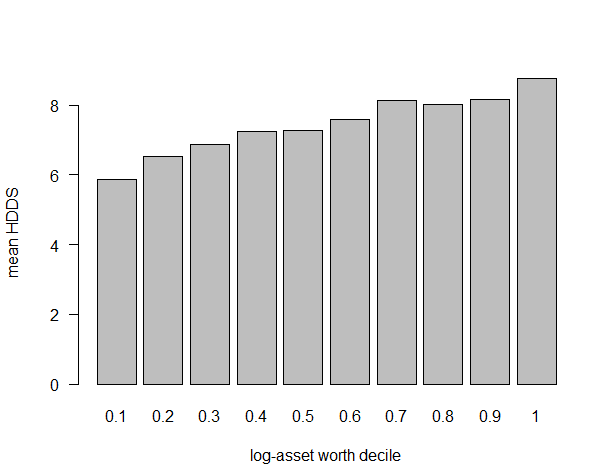
\includegraphics[width=3in]{subchapters/figures/hdds_by_lnA0}
\par\end{centering}
\caption{\label{fig:Diversity-Scores}Diversity Score changes by log asset
deciles}
\end{figure}

\begin{figure}[H]
\begin{centering}
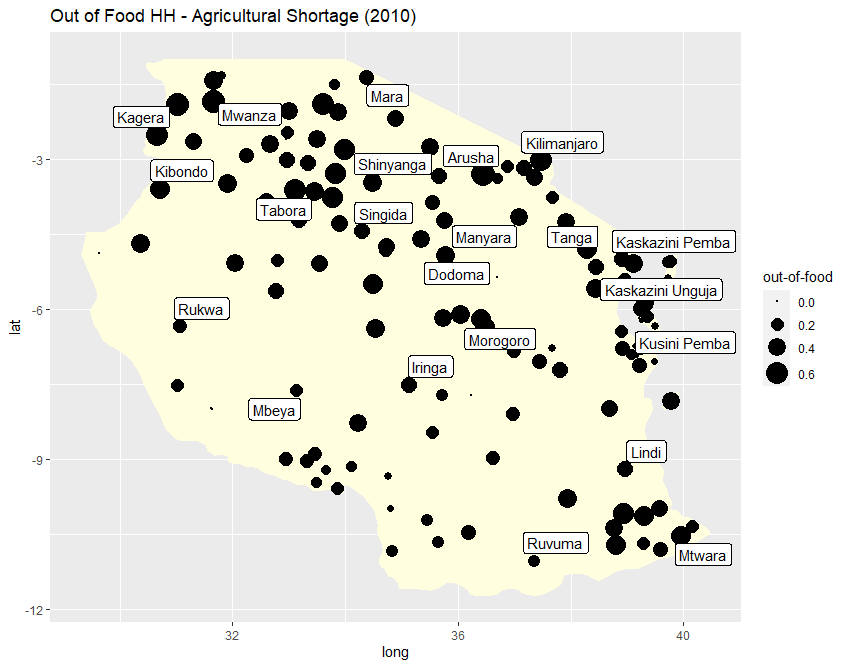
\includegraphics[width=4in]{subchapters/figures/tnz_out_food_due_to_agri_households2010}
\par\end{centering}
\caption{\label{fig:FractionAgInp}Fraction of households in Tanzania having
run of food due to agricultural inputs in the past year (2010)}
\end{figure}

\begin{figure}[H]
\begin{centering}
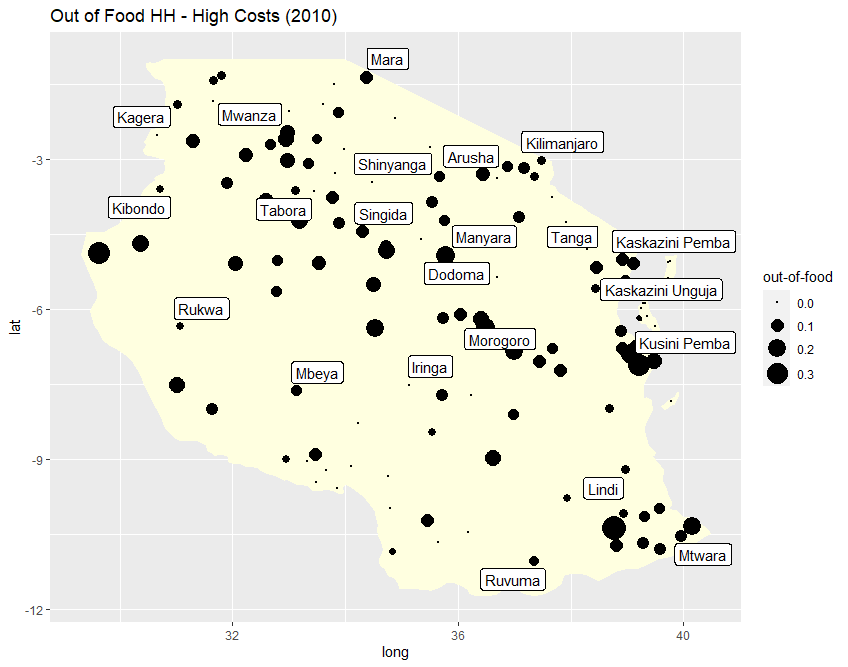
\includegraphics[width=4in]{subchapters/figures/tnz_out_food_due_to_costs_households2010}
\par\end{centering}
\caption{\label{fig:FractionHiCost}Fraction of households having run of food
due to costs in the past year (2010)}
\end{figure}

The spatial distribution of food insecurity provides us an overview
of regional disparities in the country. To survey food insecurity,
we use the directly observed food deprivation in the survey to compare
the fraction of households having run out of food (either due to lack
of agricultural inputs or high prices) in the past year across urban
and rural areas (see Figures \ref{fig:FractionAgInp} and \ref{fig:FractionHiCost}).
While the figures do suggest a significant proportion of households
running out of food in urban areas (due to high costs), the overall
hunger instances remain proportionately lower in the urban areas (when
compared to the households having run out of food due to agricultural
reasons- see Figure \ref{fig:FractionHiCost}). While the food insecurity
does not seem significantly stronger in either urban or rural areas,
the extremity of urban-rural or regional differences seems evident
from a comparison of assets and occupations. As a non-parametric view
of occupations\footnote{The variable \texttt{occupation\_rank} shown in the figure is defined
as an ordered variable indicating an income-based rank inferred from
the occupation of the head-household using the available income data
(see\textbf{ }Appendix \ref{sec:appendix_food_3} for mapping of occupations
to occupation-ranks).} and value of assets-owned show (Figure \ref{fig:occupations_r_tn}),
the higher-paid occupations seems severely to urban - particularly
eastern coastal - areas in Tanzania.

\begin{figure}[h]
\begin{centering}
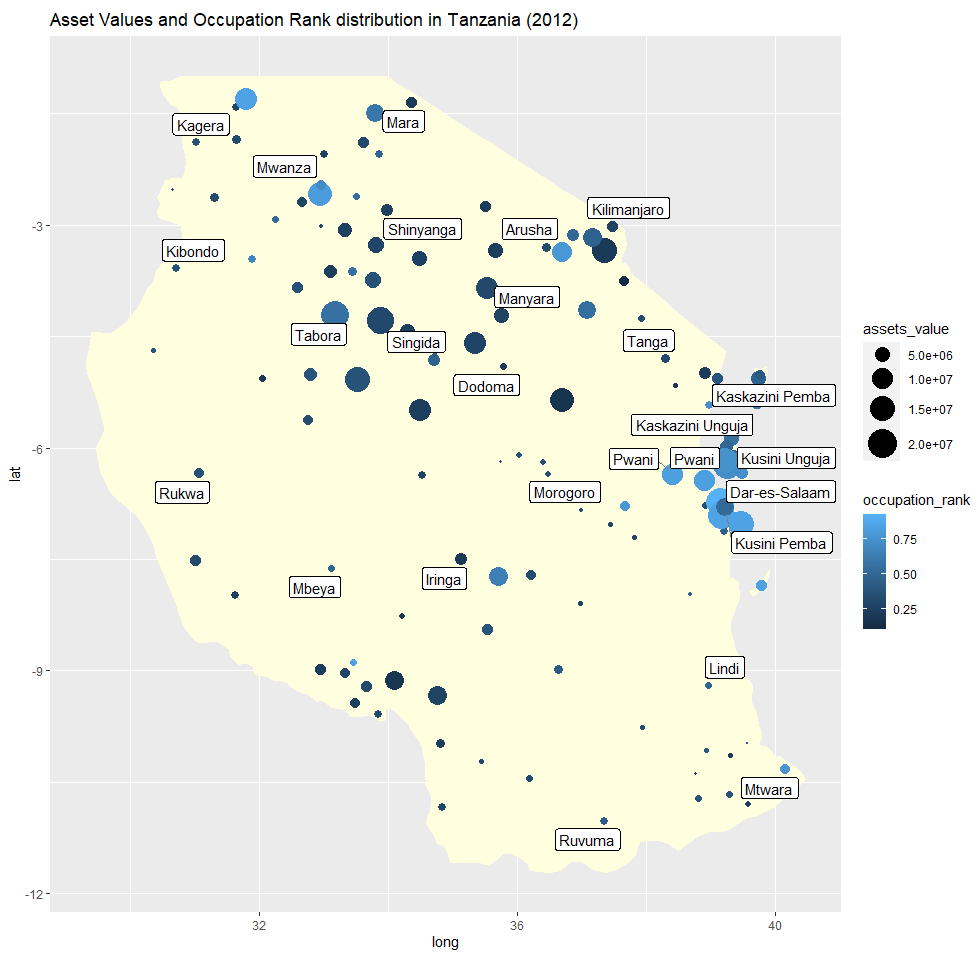
\includegraphics[width=4.5in]{subchapters/tnz_assets_occuprank_distribution_2012}
\par\end{centering}
\caption{\label{fig:occupations_r_tn}Occupations and consumer-owned assets
in Tanzania}
\end{figure}


\subsection{Results}

\noindent

The key goal of our empirical analysis is to test whether the effects
of permanent income (as well as asset-ownership) result in higher
quality overall or if the effects are limited to specific food-categories
in Tanzania. The disaggregated view of quality into commodities based
on FAO categories allows us to relate the choice for quality in high-level
commodity groups with the effects of permanent income - while also
controlling with local prices in an AIDS framework. The effect of
permanent income measures seems significant on food quality with respect
to the meats-proteins commodity. We also find that access to higher
food quality is higher in localities with access to electricity.
\begin{center}
\begin{table}[H]
\begin{centering}
\begin{tabular}{>{\raggedright}p{2in}|>{\raggedright}p{3.5in}}
\hline 
Variable & Description\tabularnewline
\hline 
\texttt{ln\_tot\_exp} & logarithm of per-head total expenditure $x_{t}$ per household \tabularnewline
\hline 
\texttt{\small{}lp-} & base-prices for various commodities\tabularnewline
\hline 
\texttt{hsize} & number of members in a household\tabularnewline
\hline 
\texttt{age} & age of the household-head\tabularnewline
\hline 
\texttt{logA} & logarithm of sum of reported market-price of assets owned by the household\tabularnewline
\hline 
\texttt{isurban} & indicator variable specifying if the region is Dar-es-Salaam, Mbeya,
Mwanza or Magharibi Unguja(Zanzibar)\tabularnewline
\hline 
\texttt{has\_electric} & indicator variable specifying if the household uses electricity or
not\tabularnewline
\end{tabular}
\par\end{centering}
\caption{\label{tab:Control-Variables}Control Variables}
\end{table}
\par\end{center}

%[Systematic introduction of control variables]

The estimation results from the AIDS formulation - which we have specified
in Equations \ref{eq:AIDS_quality_w} and \ref{eq:AIDS_quality_lnV}
- are presented in Tables \ref{results_has_electric_2014} and \ref{results_elecassets_2014}.
The logarithm of the total expenditure \texttt{\footnotesize{}ln\_tot\_exp}
is used as the main explanatory variable in the results presented
in Table \ref{results_has_electric_2014} . In an alternative formulation
for which the results presented in Table \ref{results_elecassets_2014},
the logarithm of total household owned (long-term) assets \texttt{logA}
is used as the main explanatory variable. An important set of controls
are the prices corresponding to the food commodities - which are listed
in Table \ref{tab:GroupsModified}. As described in Section \ref{subsec:Econometric-Method},
the AIDS formulation in Equations \ref{eq:AIDS_quality_w} and \ref{eq:AIDS_quality_lnV}
use the logarithm of base-prices of food categories (commodities)
as price-controls. These are represented as the variables starting
with the prefix \texttt{\footnotesize{}lp}- (e.g., \texttt{lpdensefoods,
lpnonfresh, lpprotein }etc.) in the results presented in Tables \ref{results_has_electric_2014}
and \ref{results_elecassets_2014}. Recall that the base-price $P_{G}$
for every commodity $G$ in the Equation \ref{eq:base_price_structure}
is simply the minimum price of the goods within the commodity group
that is derived from the locally observed market prices (at the district
level) rather than the unit-values (estimated by averaging expenditure
over a locality) for goods within a commodity. Every composite commodity
in the AIDS regression (see Equations \ref{eq:AIDS_quality_w} and
\ref{eq:AIDS_quality_lnV}) thus corresponds to an \texttt{\footnotesize{}lp-}
variable. It is worth remarking that the prices of other items in
the commodity are incorporated in the price-structure that is considered
in the measurement of quality. Other important controls used for results
in Tables \ref{results_has_electric_2014} and \ref{results_elecassets_2014}
are listed in Table \ref{tab:Control-Variables}. 

Of the controls in Table \ref{tab:Control-Variables}, the indicator
variable \texttt{has\_electric }- specifies whether the household
uses electricity (used in both Tables \ref{results_has_electric_2014}
and \ref{results_elecassets_2014}) and is inferred from the field
for source of energy for lighting in the survey. Two further household
characteristics which we explore the effects of are \texttt{hsize}
(number of household members ) and \texttt{age} (age of the household-head).
Whether the households reside in urban areas or not are considered
with a indicator variable \texttt{isurban} ( indicator variable for
densely populated urban areas).
\begin{center}
\begin{table}[H]
\begin{centering}
\begin{tabular}{>{\raggedright}p{2in}|>{\raggedright}p{3.5in}}
\hline 
Variable & Description\tabularnewline
\hline 
\texttt{qcereals} & budget share for the entire commodity: cereals\tabularnewline
\hline 
\texttt{qVcereals} & quality metric for the entire commodity: cereals\tabularnewline
\hline 
\texttt{qcomplements} & budget share for the entire commodity: complements\tabularnewline
\hline 
\texttt{qVcomplements} & quality metric for the entire commodity: complements\tabularnewline
\hline 
\texttt{qfat} & budget share for the entire commodity: fat\tabularnewline
\hline 
\texttt{qVfat} & quality metric for the entire commodity: fat\tabularnewline
\hline 
\texttt{qfish} & budget share for the entire commodity: fish\tabularnewline
\hline 
\texttt{qVfish} & quality metric for the entire commodity: fish\tabularnewline
\hline 
\texttt{qfruits} & budget share for the entire commodity: fruits\tabularnewline
\hline 
\texttt{qVfruits} & quality metric for the entire commodity: fruits\tabularnewline
\hline 
\texttt{qmeatsproteins} & budget share for the entire commodity: meats-proteins\tabularnewline
\hline 
\texttt{qVmeatsproteins} & quality metric for the entire commodity: meats-proteins\tabularnewline
\hline 
\texttt{qmilk} & budget share for the entire commodity: milk\tabularnewline
\hline 
\texttt{qVmilk} & quality metric for the entire commodity: milk\tabularnewline
\hline 
\texttt{qstarches} & budget share for the entire commodity: starches\tabularnewline
\hline 
\texttt{qVstarches} & quality metric for the entire commodity: starches\tabularnewline
\hline 
\texttt{qtubers} & budget share for the entire commodity: tubers\tabularnewline
\hline 
\texttt{qVtubers} & quality metric for the entire commodity: tubers\tabularnewline
\hline 
\texttt{qveg} & budget share for the entire commodity: vegetables\tabularnewline
\hline 
\texttt{qVveg} & quality metric for the entire commodity: vegetables\tabularnewline
\end{tabular}
\par\end{centering}
\caption{\label{tab:Dependent-Variables}Dependent Variables}
\end{table}
\par\end{center}

The dependent variables of the AIDS regressions in the columns of
Tables \ref{results_has_electric_2014} and \ref{results_elecassets_2014}-
starting either with \texttt{\footnotesize{}q}- or with \texttt{\footnotesize{}qV}
- indicate the budget-share and quality metric respectively. The columns
starting with \texttt{\footnotesize{}q-} indicate the budget shares
that are used as the dependent variables in AIDS regressions (see
Equation \ref{eq:AIDS_quality_w} ) while the columns starting with
\texttt{\footnotesize{}qV- }indicate the logarithm of the quality
metric as the dependent variable (i.e. $ln\ V$ in the Equation \ref{eq:AIDS_quality_lnV}).
The list of all dependent variables are presented in Table \ref{tab:Dependent-Variables}.
Recall that the classification of items - which is based on prices-correlation
- results in the commodities and constituents good listed in Table
\ref{tab:GroupsModified}. The total number of equations (the Equations
\ref{eq:AIDS_quality_w} and \ref{eq:AIDS_quality_lnV} specified
in Section \ref{subsec:Econometric-Method}) for the estimation is
therefore $10\times2=20$ (see Appendix \ref{sec:appendix_food_4}
for the entire list of estimation equations). The estimation uses
a three-stage least-squares method for systems of equations (see \cite{Zellner3SLS1992})
for the Equations \ref{eq:AIDS_quality_w} and \ref{eq:AIDS_quality_lnV}
and with symmetry constraints specified in Section \ref{subsec:Econometric-Method}.

\subsection*{Discussion}

\noindent

%[Significance of has_electric, assets and ln_tot_exp]

The results obtained from the AIDS regression shown in Tables \ref{results_has_electric_2014}
and \ref{results_elecassets_2014} suggest a relevance of permanent
income (measured with total expenditure) and ownership of assets -
along with access to electricity - on the demand for quality in food.
While there is a some heteroskedasticity in the results (tested for
with Breush-Pagan statistic), the effects of household expenditure
and total assets owned appear significant for quality.

%[Effect of ln_tot_exp]

In Table \ref{results_has_electric_2014}, the effect of permanent
income (\texttt{ln\_tot\_exp} ) is positive on quality across all
food commodities i.e. the income-elasticities are positive for quality
within food categories (commodities). This does not seem surprising
since the income-elasticities for quality are expected to be positive
so long as a higher total expenditure \texttt{ln\_tot\_exp} is spent
on the more expensive variants (goods) within a food category (commodity).
The negative income elasticities for budget-share of some food commodities
are also predictable - if we consider that certain goods are preferred
for higher (price-based) quality and therefore lower quantity (budget
share). Of particular attention is how the budget shares show a decline
with total expenditure logarithm for commodities \texttt{fat }and
\texttt{meatsproteins} (see coefficients of \texttt{ln\_tot\_exp}
under \texttt{qfat} and \texttt{qmeatsproteins} in Table \ref{results_has_electric_2014})
. More specifically, the increase in food expenditure is associated
with less quantity (at the cost of higher quality) of \texttt{fats
}and \texttt{meatsproteins} - while quality consumed for both fats
and meats-proteins rises with higher total expenditure logarithm (see
coefficients of \texttt{ln\_tot\_exp} under \texttt{qVfat} and \texttt{qVmeatsproteins}
in Table \ref{results_has_electric_2014}). With cereals, on the other
hand, we see that the budget shares rise with higher total expenditure
logarithm (see coefficient of \texttt{ln\_tot\_exp} under \texttt{qcereals}
in Table \ref{results_has_electric_2014}) while the cereals-quality
also increases with higher total expenditure logarithm (see coefficient
of \texttt{ln\_tot\_exp} under \texttt{qVcereals} in Table \ref{results_has_electric_2014}).
The demand for quality (price-based) for meat is unlike that for cereals
in the sense that higher-income households increase both price-based
quality and quantity (budget-shares) for cereals whereas they seem
increase quality without increasing quantity (budget shares) for meats.

%[has_electric in ln_tot_exp table and the endogeneity]

Looking at the effect of access to electricity ( \texttt{has\_electric}
) in Table \ref{results_has_electric_2014}, we see a higher quality
across food categories - an effect similar to that of total expenditure
logarithm \texttt{ln\_tot\_exp }(except for fats where quality is
not significantly higher for consumers with access to electricity).
It could be argued that having access to electricity is endogenous
with higher prosperity. Thus it may simply be that those with higher
income are the one with access to electricity and have a better access
to quality through ownership of electric appliances. However, the
correlation of having access to electricity with prosperity is more
likely through being in the urban area rather through income. This
is because the indicator variable \texttt{has\_electric }used for
access to electricity is based only on the usage of electricity as
the primary source of lighting at home. The basic usage of electricity
hardly reflects the income of the household - and is more strongly
correlated with being in an area (more often urban) where electricity
is available (particularly given the sparse distribution of electricity
in Tanzania). Since availability of refrigeration facilities in a
market may improve the availability of fruits and meats in a wider
area, the positive externality through being in richer areas - one
that includes access to electricity - is more likely to be the cause
for higher quality in food categories.

%[ln_tot_exp table - hsize ]

The effects of \texttt{hsize} on quality are also worth noting - as
larger families (higher \texttt{hsize} ) corresponds to lower quality
(particularly in protein and fruits-veg) but lower their budget-share
for consumption. This may struggle in maintaining high quality in
larger families with children.

%[ln_tot_exp table - prices]

% g <- merge((subset(o2014,household_status==1))[,c("hhid","isurbanp","lightingfuel")],g2014,by=c("hhid"))
% g$has_electric  <- with(g,as.integer(is.element(lightingfuel,c(1,8))))
% ddply(subset(g,category=="meatsproteins"),.(isurbanp),summarise,n=median(tot_categ_exp/lp_min_price))
% fdf <- get_fao_quality_agg_df()
% fdf$logA <- log(fdf$all_assets_mtm+1e-7)
% gf <- (subset(merge(fdf[,c("hhid","logA")],g,by=c("hhid"))))
% k <- subset(gf,isurbanp==T & category=="meatsproteins") ; plot(k$logA, with(k,tot_categ_exp/lp_min_price),xlim=c(2,3.2)) 
% the asset dependence does not change - this is not apparent from the descriptive statistics

A key advantage of using the proposed framework of quality is that
it allows us to examine the effect of prices of commodities on quality.
Looking at the effect of (base-)prices (variables \texttt{lp-}) in
both Tables \ref{results_has_electric_2014} and \ref{results_elecassets_2014},
we see with \texttt{lpmeatsproteins} - for example - that the high
base-price of meats-proteins (the cheapest meat-protein available
in the district) corresponds to higher quality in \texttt{fruits}
and \texttt{veg}. Thus, the households in districts where base-price
of \texttt{meatsproteins }(price of cheapest meat-protein) is high
also avail higher quality of fruits and veg - an indication of how
meat consumption may be associated with higher income in Tanzania. 

The results in Table \ref{results_has_electric_2014} also suggest
certain substitutions in quality across some food commodities. For
example, with a rise in prices of cereals (\texttt{lpcereals}), the
quality in meats-proteins (see coefficient of \texttt{lpcereals} under
\texttt{qVmeatsproteins} in Table \ref{results_has_electric_2014})
increases but the quality in starches (see coefficient of \texttt{lpcereals}
under \texttt{qVstarches} in Table \ref{results_has_electric_2014})
and vegetables (see coefficient of \texttt{lpcereals} under \texttt{qVveg
}in Table \ref{results_has_electric_2014} ) declines - indicating
that the consumers tend to increase quality in meat-consumption while
reducing the quality for starches and veg. In other words, with higher
prices of (cheapest) meat, the consumer is more likely to increase
quality elsewhere (e.g., in fruits and vegetables) - indicating once
again how meat consumption rises with higher income.

On similar lines, we see that the quality in starches seems to drop
with rise in prices of fruits (see coefficient of \texttt{lpfruits}
under \texttt{qVstarches} in Table \ref{results_has_electric_2014})
whereas the quality in fruits does not rise with the base-price of
starches (see coefficient of \texttt{lpstarches} under \texttt{qVfruits}
in Table \ref{results_has_electric_2014}). In other words, when (cheapest)
fruit is more expensive, starch quality is also lower for consumers
whereas (cheapest) starch being more expensive does not raise the
quality of fruits for consumers. It is more often thus that the consumers
spend higher on quality in starches when the fruits become expensive
(rather than spending higher on quality in fruits when starch becomes
more expensive). A similar relation is not seen between tubers and
starches whose consumption of quality seem to move together.

The observation from the budget shares that the expenditure on \texttt{veg}
and \texttt{meatsproteins} is higher - particularly for \texttt{meatsproteins}
- in urban areas can also be verified with a simple calculation of
total expenditure divided by the commodity base-price. Estimating
the effective quantity of \texttt{meatsproteins} consumed as the \texttt{meatsproteins}
expenditure divided by its base-price, the urban areas seem to consume
about 1.61 times more \texttt{meatsproteins} and spend 1.63 times
more (comparing just expenditure) - not as much for the expenditure
on \texttt{chicken} or \texttt{fish}. With effective quantity of \texttt{veg},
the urban areas consume about 1.1 times more \texttt{meatsproteins}
and spend also about 1.1 times more than the rural areas. Looking
at the expenditures in urban and rural areas for \texttt{cereals},
we see that unlike with \texttt{meatsproteins}, the differences in
expenditure (or in effective quantity) for \texttt{cereals} across
urban and rural areas and are not wide. The expenditures also suggest
that while the consumption of \texttt{veg} rises with total expenditure
logarithm \texttt{ln\_tot\_exp} , it does not rise as much as \texttt{meatsproteins}
in urban areas and does not differ a lot from the expenditures in
rural areas.

%[assets-table]

In Table \ref{results_elecassets_2014} - where total assets logarithm
\texttt{logA} is used as the main explanatory variable instead of
total expenditure \texttt{ln\_tot\_exp} - the coefficient of total
assets logarithm is positive for meatsproteins (dependent variable:
\texttt{qmeatsproteins}) - suggesting that those with lower assets
do consume less \texttt{meatsproteins }overall. In other words, the
lower quantity of \texttt{meatsproteins }for those with low-assets-ownership
does not mean a higher quality in \texttt{meatsproteins }(compare
signs under \texttt{qmeatsproteins} of the coefficients for \texttt{logA}
and \texttt{ln\_tot\_exp} in Tables \ref{results_has_electric_2014}
and \ref{results_elecassets_2014} ). The quality consumed for meats-proteins
does rise with higher total assets logarithm as well. Comparing with
cereals, on the other hand, we see that the budget shares are lower
for those with higher total assets - even though the quality consumed
is higher.

The access to electricity ( \texttt{has\_electric} ) indicates a higher
quality across food categories in Table \ref{results_elecassets_2014}
as well. The budget shares rise for fruits and milk in Table \ref{results_elecassets_2014}
whereas they fall for fat (\texttt{qfat}) and meatsproteins (\texttt{qmeatsproteins})
- even though the quality metrics rise (both \texttt{qVfat} and \texttt{qVmeatsproteins})
for the consumers having electricity. This may be due to refrigeration
storage facilities available in certain localities. The consumption
of fish (budget shares \texttt{qfish}) is not affected by the \texttt{has\_electric
}variable as much as \texttt{meatsproteins} - suggesting a higher
local consumption for fish (likely less dependent on refrigeration
facilities overall). For fruits and milk on the other hand, both the
quality consumed and budget-share are higher for consumers with access
to electricity (see Table \ref{results_elecassets_2014}).

%[Both Tables - isurban and hsize]

In both Tables \ref{results_has_electric_2014} and \ref{results_elecassets_2014},
we see that the effect of \texttt{isurban} (apart from the base-price
$P_{G}$) on quality is significant on quality across all food categories.
This could be an indication of higher income occupations concentrated
in the eastern coast and centre of Tanzania. More specifically, quality
for meatsproteins ( \texttt{qVmeatsproteins} ) is slightly lower in
urban areas (compare coefficients of \texttt{isurban} under \texttt{qVmeatsproteins}
and \texttt{qVfruits} in both Tables \ref{results_has_electric_2014}
and \ref{results_elecassets_2014}) and is better with access to electricity.
In other words, those with no access to electricity in the urban areas
are less likely to spend higher on quality of meats-proteins compared
to the consumers in rural areas. The effects of both total expenditure
and assets-ownership are significant in the quality of consumption
for food. The access to electricity in urban environment creates clear
differences in lifestyle choices as well as dependence on higher budgets
- an effect that remains significant for access to quality in nutrition.
In summary, even though there may be some positive externality with
being in the urban areas, the differences in quality of consumption
associated with high permanent income as well as assets possession
remain significant. 

While the question of whether higher quality for food can be considered
aspirational or not could be answered only after surveys of subjective
well-being of consumers, there are two observations pertaining to
determinants of aspirational consumption that we can make from the
above results. First, the demand for quality is strong for specific
food items (rather than across wider nutritional categories). Second,
the role of regional identity is likely to be strong towards aspirational
consumption due to the extreme life-style differences between urban
and rural areas. The observations seem to be supported by the presence
of a strong positive externality with rich surroundings in the data
on subjective-welfare in LSMS survey in Tanzania as well \cite{AstebiCarbonell2019}.

%The consumption such as food, where a higher quality may be always in the market, it is always difficult and therefore the processes of snob becoming a bandwagon is less of a concern.

%[Robustness]

\subsection*{Robustness Checks}

\noindent

As a test of the robustness of results, we calculate the food-quality
using the market-provided prices and instead of the expenditure reported
by the household. More specifically, in the results shown in Tables
\ref{results_has_electric_2014} and \ref{results_elecassets_2014},
we have used diary-costs on goods as reported by the household - costs
that are recorded by the LSMS for the goods that were consumed from
purchases in the last week. If a household didn't purchase anything
in the past week, there would only be quantities consumed (not costs)
that would be reported for the household in the diary. Since we have
the market-prices available, another way to calculate costs, budget-shares
and quality would be to infer costs as the multiple of market-prices
from the quantities consumed in the past week (which is reported for
all households regardless of whether they had purchased something
in the last week or not). Recalculating quality and budget shares
still shows us the same economic and statistical significance (results
available on request) of electricity and household assets in quality
of food categories (commodities).

% The education rank is set to 1 for all pre-primary levels, to rank 2 for until the completion of primary education, to rank 3 for up to the secondary education level and to 4 for all higher education levels (higher-secondary, university etc.). For instance, the primary school leaving exam is taken at D7 in Tanzania and corresponds to the education rank 2 ; all standards above D7 correspond to the education rank 3 and so forth. The complete mapping is provided in Table \ref{education_rank_tnz}. The argument for using the education-ranks as instruments is simply that a higher food quality in food is unlikely to be favoured by differences in education levels. In other words, while quality - in general - could be constrained due to occupational structures in the economy, there are few reasons to think that purchases of food could be influenced by one's education level except through the permanent income measure.

% Add - \rowcolor{Gray} after \\ 

\begin{landscape}
\begin{table}
\caption{\label{results_has_electric_2014}reg3 results with electricity usage indicator control (2014)} 
\resizebox{\columnwidth}{!}{

\def\sym#1{\ifmmode^{#1}\else\(^{#1}\)\fi} \begin{tabular}{l*{21}{c}} \hline\hline  & \multicolumn{1}{c}{} & \multicolumn{1}{c}{(1)} & \multicolumn{1}{c}{(2)} & \multicolumn{1}{c}{(3)} & \multicolumn{1}{c}{(4)} & \multicolumn{1}{c}{(5)} & \multicolumn{1}{c}{(6)} & \multicolumn{1}{c}{(7)} & \multicolumn{1}{c}{(8)} & \multicolumn{1}{c}{(9)} & \multicolumn{1}{c}{(10)} & \multicolumn{1}{c}{(11)} & \multicolumn{1}{c}{(12)} & \multicolumn{1}{c}{(13)} & \multicolumn{1}{c}{(14)} & \multicolumn{1}{c}{(15)} & \multicolumn{1}{c}{(16)} & \multicolumn{1}{c}{(17)} & \multicolumn{1}{c}{(18)} & \multicolumn{1}{c}{(19)} & \multicolumn{1}{c}{(20)} \\ & \multicolumn{1}{c}{} & \multicolumn{1}{c}{qcereals} & \multicolumn{1}{c}{qcomplements} & \multicolumn{1}{c}{qfat} & \multicolumn{1}{c}{qfish} & \multicolumn{1}{c}{qfruits} & \multicolumn{1}{c}{qmeatsproteins} & \multicolumn{1}{c}{qmilk} & \multicolumn{1}{c}{qstarches} & \multicolumn{1}{c}{qtubers} & \multicolumn{1}{c}{qVcereals} & \multicolumn{1}{c}{qVcomplements} & \multicolumn{1}{c}{qveg} & \multicolumn{1}{c}{qVfat} & \multicolumn{1}{c}{qVfish} & \multicolumn{1}{c}{qVfruits} & \multicolumn{1}{c}{qVmeatsproteins} & \multicolumn{1}{c}{qVmilk} & \multicolumn{1}{c}{qVstarches} & \multicolumn{1}{c}{qVtubers} & \multicolumn{1}{c}{qVveg}\\ \hline
\\ \rowcolor{Gray}  & isurban & -0.0317$^{***}$ & -0.0170$^{***}$ & 0.0002 & 0.0197$^{***}$ & 0.0094$^{*}$ & 0.0118 & -0.0041$^{*}$ & 0.0074$^{**}$ & -0.0039 & -0.1542$^{**}$ & 0.0360 & 0.0055$^{*}$ & -0.8281 & 0.0484$^{*}$ & 0.1402$^{**}$ & -0.4567$^{***}$ & -0.0581$^{***}$ & 0.0190 & 0.0577 & 0.1297$^{***}$\\ \rowcolor{Gray} &  & (0.000) & (0.000) & (0.964) & (0.000) & (0.020) & (0.120) & (0.043) & (0.007) & (0.260) & (0.004) & (0.104) & (0.021) & (0.283) & (0.011) & (0.003) & (0.000) & (0.000) & (0.764) & (0.121) & (0.000)
\\ & has\_electric & -0.0641$^{***}$ & -0.0095$^{*}$ & 0.0019 & -0.0050 & 0.0253$^{***}$ & 0.0296$^{***}$ & 0.0066$^{**}$ & 0.0175$^{***}$ & -0.0041 & 0.0828 & 0.0294 & -0.0008 & -1.4587 & 0.0367 & 0.2107$^{***}$ & 0.4544$^{***}$ & 0.0939$^{***}$ & 0.5391$^{***}$ & 0.1254$^{**}$ & 0.1341$^{***}$\\ &  & (0.000) & (0.029) & (0.653) & (0.398) & (0.000) & (0.000) & (0.002) & (0.000) & (0.278) & (0.136) & (0.206) & (0.767) & (0.071) & (0.069) & (0.000) & (0.000) & (0.000) & (0.000) & (0.001) & (0.000)
\\ \rowcolor{Gray} & hh\_age & 0.0002 & 0.0002 & -0.0003$^{**}$ & 0.0004$^{*}$ & -0.0002$^{*}$ & 0.0002 & -0.0000 & -0.0001 & -0.0002$^{*}$ & 0.0023 & 0.0008 & 0.0000 & -0.0081 & -0.0005 & -0.0027$^{*}$ & 0.0044$^{**}$ & -0.0003 & -0.0019 & -0.0024$^{*}$ & -0.0013$^{**}$\\ \rowcolor{Gray} &  & (0.407) & (0.057) & (0.009) & (0.015) & (0.020) & (0.274) & (0.560) & (0.301) & (0.044) & (0.100) & (0.180) & (0.883) & (0.688) & (0.321) & (0.028) & (0.003) & (0.403) & (0.253) & (0.015) & (0.004)\\ & hsize & -0.0035$^{**}$ & 0.0042$^{***}$ & 0.0026$^{***}$ & 0.0038$^{***}$ & -0.0018$^{**}$ & -0.0003 & -0.0014$^{***}$ & -0.0009$^{*}$ & -0.0004 & -0.0887$^{***}$ & -0.0310$^{***}$ & -0.0009$^{*}$ & 0.2308$^{*}$ & 0.0000 & -0.0484$^{***}$ & -0.0574$^{***}$ & -0.0141$^{***}$ & -0.0294$^{**}$ & -0.0228$^{***}$ & -0.0208$^{***}$\\ &  & (0.004) & (0.000) & (0.000) & (0.000) & (0.003) & (0.808) & (0.000) & (0.029) & (0.478) & (0.000) & (0.000) & (0.011) & (0.049) & (0.994) & (0.000) & (0.000) & (0.000) & (0.002) & (0.000) & (0.000)\\ \rowcolor{Gray} & ln\_tot\_exp & 0.0641$^{***}$ & -0.0091$^{***}$ & -0.0326$^{***}$ & -0.0052$^{*}$ & 0.0095$^{***}$ & -0.0532$^{***}$ & 0.0042$^{***}$ & 0.0112$^{***}$ & 0.0049$^{**}$ & 0.6292$^{***}$ & 0.2089$^{***}$ & -0.0002 & 0.6893$^{*}$ & 0.1220$^{***}$ & 0.3857$^{***}$ & 0.5941$^{***}$ & 0.0799$^{***}$ & 0.4104$^{***}$ & 0.1870$^{***}$ & 0.1455$^{***}$\\ \rowcolor{Gray} &  & (0.000) & (0.000) & (0.000) & (0.025) & (0.000) & (0.000) & (0.000) & (0.000) & (0.001) & (0.000) & (0.000) & (0.855) & (0.032) & (0.000) & (0.000) & (0.000) & (0.000) & (0.000) & (0.000) & (0.000)\\ & lpcereals & -0.0060 & 0.0001 & -0.0014 & 0.0031 & 0.0166$^{***}$ & -0.0166$^{***}$ & -0.0011 & 0.0023 & 0.0049$^{**}$ & -1.5037$^{***}$ & 0.0516$^{**}$ & -0.0018 & 0.6404 & 0.0194 & 0.0237 & 0.3641$^{***}$ & -0.0228$^{*}$ & -0.1978$^{***}$ & -0.0431 & -0.0503$^{***}$\\ &  & (0.253) & (0.970) & (0.397) & (0.187) & (0.000) & (0.000) & (0.252) & (0.133) & (0.002) & (0.000) & (0.001) & (0.217) & (0.247) & (0.100) & (0.477) & (0.000) & (0.012) & (0.000) & (0.088) & (0.000)\\ \rowcolor{Gray} & lpcomplements & 0.0001 & 0.0019 & 0.0003 & -0.0012 & 0.0016 & 0.0060 & -0.0005 & 0.0015 & -0.0066$^{***}$ & 1.5261$^{***}$ & -0.0461 & -0.0031 & 4.4315$^{**}$ & -0.0882$^{**}$ & 0.0245 & 1.7650$^{***}$ & 0.0163 & 0.4861$^{***}$ & 0.0484 & -0.1422$^{***}$\\\rowcolor{Gray}  &  & (0.970) & (0.805) & (0.768) & (0.429) & (0.615) & (0.273) & (0.522) & (0.263) & (0.000) & (0.000) & (0.260) & (0.058) & (0.002) & (0.001) & (0.767) & (0.000) & (0.419) & (0.000) & (0.440) & (0.000)\\ & lpfat & -0.0014 & 0.0003 & 0.0002 & 0.0013 & -0.0020$^{*}$ & 0.0032 & -0.0008 & -0.0019$^{**}$ & 0.0013 & -0.0110 & -0.0236$^{***}$ & -0.0002 & -8.8267$^{***}$ & 0.0064 & 0.0098 & -0.0016 & -0.0028 & -0.1016$^{***}$ & 0.0115 & -0.0025\\ &  & (0.397) & (0.768) & (0.850) & (0.202) & (0.044) & (0.075) & (0.077) & (0.003) & (0.065) & (0.419) & (0.000) & (0.714) & (0.000) & (0.156) & (0.426) & (0.916) & (0.423) & (0.000) & (0.224) & (0.590)\\ \rowcolor{Gray} & lpfish & 0.0031 & -0.0012 & 0.0013 & 0.0052$^{*}$ & -0.0027 & -0.0041 & -0.0023$^{***}$ & -0.0015 & 0.0030$^{**}$ & 0.0100 & -0.0214$^{*}$ & -0.0007 & -0.4615 & 0.0413$^{***}$ & 0.0326 & -0.0128 & -0.0078 & 0.0209 & 0.0306$^{*}$ & 0.0004\\ \rowcolor{Gray} &  & (0.187) & (0.429) & (0.202) & (0.013) & (0.059) & (0.110) & (0.000) & (0.104) & (0.003) & (0.606) & (0.011) & (0.382) & (0.111) & (0.000) & (0.063) & (0.542) & (0.116) & (0.374) & (0.023) & (0.946)\\ & lpfruits & 0.0166$^{***}$ & 0.0016 & -0.0020$^{*}$ & -0.0027 & 0.0079$^{*}$ & -0.0243$^{***}$ & 0.0015$^{*}$ & 0.0023$^{*}$ & 0.0005 & 0.0458 & -0.0046 & -0.0013 & -0.9906 & -0.0084 & -0.3593$^{***}$ & -0.0227 & -0.0027 & -0.1496$^{**}$ & -0.0263 & -0.0169\\ &  & (0.000) & (0.615) & (0.044) & (0.059) & (0.010) & (0.000) & (0.028) & (0.043) & (0.632) & (0.259) & (0.795) & (0.301) & (0.112) & (0.498) & (0.000) & (0.601) & (0.773) & (0.002) & (0.343) & (0.195)\\ \rowcolor{Gray} & lpmeatsproteins & -0.0166$^{***}$ & 0.0060 & 0.0032 & -0.0041 & -0.0243$^{***}$ & 0.0382$^{***}$ & 0.0017 & -0.0054$^{**}$ & -0.0044$^{*}$ & -0.0368 & 0.0432 & 0.0058$^{**}$ & 8.0136$^{***}$ & 0.0343 & 0.1864$^{**}$ & -2.2568$^{***}$ & 0.0109 & -0.0440 & -0.0364 & 0.1751$^{***}$\\ \rowcolor{Gray} &  & (0.000) & (0.273) & (0.075) & (0.110) & (0.000) & (0.000) & (0.153) & (0.003) & (0.012) & (0.593) & (0.153) & (0.002) & (0.000) & (0.104) & (0.003) & (0.000) & (0.486) & (0.597) & (0.438) & (0.000)\\ & lpmilk & -0.0011 & -0.0005 & -0.0008 & -0.0023$^{***}$ & 0.0015$^{*}$ & 0.0017 & 0.0019$^{***}$ & 0.0001 & -0.0014$^{**}$ & 0.0094 & -0.0048 & 0.0009$^{*}$ & -0.2357 & -0.0076$^{*}$ & 0.0283$^{**}$ & -0.0062 & 0.0176$^{***}$ & 0.0107 & 0.0017 & 0.0032\\ &  & (0.252) & (0.522) & (0.077) & (0.000) & (0.028) & (0.153) & (0.000) & (0.752) & (0.001) & (0.333) & (0.257) & (0.023) & (0.109) & (0.016) & (0.001) & (0.554) & (0.000) & (0.369) & (0.806) & (0.330)\\\rowcolor{Gray}  & lpstarches & 0.0023 & 0.0015 & -0.0019$^{**}$ & -0.0015 & 0.0023$^{*}$ & -0.0054$^{**}$ & 0.0001 & 0.0032$^{**}$ & -0.0002 & 0.0228 & 0.0239$^{**}$ & -0.0003 & -0.2865 & 0.0002 & 0.0124 & 0.0015 & -0.0043 & -0.0307 & -0.0022 & -0.0020\\ \rowcolor{Gray} &  & (0.133) & (0.263) & (0.003) & (0.104) & (0.043) & (0.003) & (0.752) & (0.001) & (0.699) & (0.173) & (0.001) & (0.598) & (0.260) & (0.962) & (0.415) & (0.936) & (0.293) & (0.145) & (0.852) & (0.715)\\ & lptubers & 0.0049$^{**}$ & -0.0066$^{***}$ & 0.0013 & 0.0030$^{**}$ & 0.0005 & -0.0044$^{*}$ & -0.0014$^{**}$ & -0.0002 & 0.0037$^{***}$ & -0.0097 & 0.0020 & -0.0007 & -0.6671$^{**}$ & 0.0180$^{***}$ & -0.0171 & 0.0468$^{**}$ & -0.0108$^{**}$ & -0.0172 & 0.0179 & 0.0015\\ &  & (0.002) & (0.000) & (0.065) & (0.003) & (0.632) & (0.012) & (0.001) & (0.699) & (0.000) & (0.479) & (0.730) & (0.234) & (0.001) & (0.000) & (0.169) & (0.002) & (0.002) & (0.303) & (0.073) & (0.753)
\\ \rowcolor{Gray} & lpveg & -0.0018$^{***}$ & -0.0031$^{***}$ & -0.0002$^{***}$ & -0.0007$^{***}$ & -0.0013 & 0.0058$^{***}$ & 0.0009$^{*}$ & -0.0003$^{***}$ & -0.0007 & -0.0530$^{***}$ & -0.0202$^{***}$ & 0.0014$^{**}$ & -1.6173 & -0.0154$^{***}$ & 0.0586$^{***}$ & 0.1228$^{***}$ & 0.0062$^{***}$ & 0.0231$^{***}$ & -0.0021$^{***}$ & 0.0337$^{***}$
\\ \rowcolor{Gray} &  & (0.217) & (0.058) & (0.714) & (0.382) & (0.301) & (0.002) & (0.023) & (0.598) & (0.234) & (0.011) & (0.028) & (0.157) & (0.000) & (0.017) & (0.002) & (0.000) & (0.205) & (0.365) & (0.886) & (0.000)
\\ & \_cons & -0.6042$^{***}$ & 0.1824$^{***}$ & 0.5310$^{***}$ & 0.1178$^{***}$ & -0.0430 & 0.9945$^{***}$ & -0.0289$^{*}$ & -0.1060$^{***}$ & -0.0190 & -8.3633$^{***}$ & -1.7428$^{***}$ & 0.0398$^{**}$ & -2.3817 & -1.0892$^{***}$ & -4.0316$^{***}$ & -6.9911$^{***}$ & -0.8506$^{***}$ & -5.2349$^{***}$ & -2.0281$^{***}$ & -1.2673$^{***}$\\ &  & (0.000) & (0.000) & (0.000) & (0.000) & (0.068) & (0.000) & (0.012) & (0.000) & (0.347) & (0.000) & (0.000) & (0.004) & (0.623) & (0.000) & (0.000) & (0.000) & (0.000) & (0.000) & (0.000) & (0.000)

\\ \hline\hline  \multicolumn{2}{l}{\footnotesize \textit{p}-values in parentheses}\\ \multicolumn{2}{l}{\footnotesize \sym{*} \(p<0.05\), \sym{**} \(p<0.01\), \sym{***} \(p<0.001\)}\\ \end{tabular}

}
\end{table} \end{landscape} 


\begin{landscape}
\begin{table}
\caption{\label{results_elecassets_2014}reg3 results with total assets (logarithm) and electricity usage indicator control  (2014)}
\resizebox{\columnwidth}{!}{

\def\sym#1{\ifmmode^{#1}\else\(^{#1}\)\fi} \begin{tabular}{l*{21}{c}} \hline\hline  & \multicolumn{1}{c}{} & \multicolumn{1}{c}{(1)} & \multicolumn{1}{c}{(2)} & \multicolumn{1}{c}{(3)} & \multicolumn{1}{c}{(4)} & \multicolumn{1}{c}{(5)} & \multicolumn{1}{c}{(6)} & \multicolumn{1}{c}{(7)} & \multicolumn{1}{c}{(8)} & \multicolumn{1}{c}{(9)} & \multicolumn{1}{c}{(10)} & \multicolumn{1}{c}{(11)} & \multicolumn{1}{c}{(12)} & \multicolumn{1}{c}{(13)} & \multicolumn{1}{c}{(14)} & \multicolumn{1}{c}{(15)} & \multicolumn{1}{c}{(16)} & \multicolumn{1}{c}{(17)} & \multicolumn{1}{c}{(18)} & \multicolumn{1}{c}{(19)} & \multicolumn{1}{c}{(20)} \\ & \multicolumn{1}{c}{} & \multicolumn{1}{c}{qcereals} & \multicolumn{1}{c}{qcomplements} & \multicolumn{1}{c}{qfat} & \multicolumn{1}{c}{qfish} & \multicolumn{1}{c}{qfruits} & \multicolumn{1}{c}{qmeatsproteins} & \multicolumn{1}{c}{qmilk} & \multicolumn{1}{c}{qstarches} & \multicolumn{1}{c}{qtubers} & \multicolumn{1}{c}{qVcereals} & \multicolumn{1}{c}{qVcomplements} & \multicolumn{1}{c}{qveg} & \multicolumn{1}{c}{qVfat} & \multicolumn{1}{c}{qVfish} & \multicolumn{1}{c}{qVfruits} & \multicolumn{1}{c}{qVmeatsproteins} & \multicolumn{1}{c}{qVmilk} & \multicolumn{1}{c}{qVstarches} & \multicolumn{1}{c}{qVtubers} & \multicolumn{1}{c}{qVveg}\\ \hline

\\ \rowcolor{Gray} & isurban & -0.0134 & -0.0197$^{***}$ & -0.0062 & 0.0194$^{***}$ & 0.0104$^{**}$ & -0.0028 & -0.0040$^{*}$ & 0.0079$^{**}$ & -0.0024 & -0.0367 & 0.0658$^{**}$ & 0.0058$^{*}$ & -0.7816 & 0.0705$^{***}$ & 0.2010$^{***}$ & -0.3775$^{***}$ & -0.0484$^{**}$ & 0.0675 & 0.0893$^{*}$ & 0.1544$^{***}$\\ \rowcolor{Gray} &  & (0.111) & (0.000) & (0.133) & (0.000) & (0.009) & (0.724) & (0.044) & (0.004) & (0.484) & (0.526) & (0.005) & (0.015) & (0.310) & (0.000) & (0.000) & (0.000) & (0.001) & (0.295) & (0.018) & (0.000)\\ & has\_electric & -0.0047 & -0.0210$^{***}$ & -0.0211$^{***}$ & -0.0043 & 0.0298$^{***}$ & -0.0172$^{*}$ & 0.0078$^{***}$ & 0.0217$^{***}$ & 0.0018 & 0.4745$^{***}$ & 0.1259$^{***}$ & 0.0003 & -1.3344 & 0.1183$^{***}$ & 0.4277$^{***}$ & 0.7374$^{***}$ & 0.1332$^{***}$ & 0.7203$^{***}$ & 0.2375$^{***}$ & 0.2203$^{***}$\\ &  & (0.594) & (0.000) & (0.000) & (0.457) & (0.000) & (0.034) & (0.000) & (0.000) & (0.635) & (0.000) & (0.000) & (0.911) & (0.094) & (0.000) & (0.000) & (0.000) & (0.000) & (0.000) & (0.000) & (0.000)\\ \rowcolor{Gray} & logA & -0.0077$^{***}$ & 0.0042$^{***}$ & -0.0016 & -0.0043$^{***}$ & 0.0021$^{*}$ & 0.0045$^{**}$ & 0.0014$^{**}$ & 0.0031$^{***}$ & -0.0019$^{*}$ & 0.0633$^{***}$ & 0.0464$^{***}$ & -0.0010$^{*}$ & 0.2649 & 0.0042 & 0.0521$^{***}$ & 0.1156$^{***}$ & 0.0146$^{***}$ & 0.0958$^{***}$ & 0.0191$^{*}$ & 0.0156$^{***}$\\ \rowcolor{Gray} &  & (0.000) & (0.000) & (0.084) & (0.000) & (0.013) & (0.008) & (0.001) & (0.000) & (0.015) & (0.000) & (0.000) & (0.049) & (0.105) & (0.316) & (0.000) & (0.000) & (0.000) & (0.000) & (0.018) & (0.000)\\ & hh\_age & -0.0001 & 0.0002 & -0.0000 & 0.0005$^{**}$ & -0.0004$^{**}$ & 0.0005$^{*}$ & -0.0001 & -0.0002$^{**}$ & -0.0002 & -0.0036$^{*}$ & -0.0018$^{**}$ & 0.0000 & -0.0196 & -0.0015$^{**}$ & -0.0067$^{***}$ & -0.0027 & -0.0012$^{**}$ & -0.0071$^{***}$ & -0.0042$^{***}$ & -0.0027$^{***}$\\ &  & (0.775) & (0.123) & (0.910) & (0.001) & (0.001) & (0.026) & (0.077) & (0.002) & (0.062) & (0.019) & (0.003) & (0.584) & (0.339) & (0.006) & (0.000) & (0.096) & (0.002) & (0.000) & (0.000) & (0.000)\\ \rowcolor{Gray} & hsize & 0.0036$^{**}$ & 0.0024$^{***}$ & 0.0003 & 0.0045$^{***}$ & -0.0016$^{*}$ & -0.0058$^{***}$ & -0.0014$^{***}$ & -0.0008 & 0.0005 & -0.0519$^{***}$ & -0.0249$^{***}$ & -0.0007 & 0.2275 & 0.0094$^{**}$ & -0.0289$^{***}$ & -0.0355$^{***}$ & -0.0109$^{***}$ & -0.0187 & -0.0117 & -0.0124$^{***}$\\ \rowcolor{Gray} &  & (0.008) & (0.000) & (0.673) & (0.000) & (0.015) & (0.000) & (0.000) & (0.091) & (0.387) & (0.000) & (0.000) & (0.071) & (0.061) & (0.003) & (0.000) & (0.000) & (0.000) & (0.067) & (0.052) & (0.000)\\ & lpcereals & 0.0015 & -0.0017 & -0.0082$^{***}$ & 0.0024 & 0.0189$^{***}$ & -0.0221$^{***}$ & 0.0001 & 0.0056$^{***}$ & 0.0057$^{***}$ & -1.4272$^{***}$ & 0.0747$^{***}$ & -0.0021 & 0.6073 & 0.0339$^{**}$ & 0.0758$^{*}$ & 0.4352$^{***}$ & -0.0096 & -0.1343$^{**}$ & -0.0203 & -0.0341$^{**}$\\ &  & (0.788) & (0.560) & (0.000) & (0.324) & (0.000) & (0.000) & (0.913) & (0.000) & (0.000) & (0.000) & (0.000) & (0.163) & (0.272) & (0.006) & (0.028) & (0.000) & (0.299) & (0.003) & (0.430) & (0.008)\\ \rowcolor{Gray} & lpcomplements & -0.0017 & 0.0030 & 0.0017 & -0.0008 & 0.0001 & 0.0076 & -0.0009 & 0.0004 & -0.0066$^{***}$ & 1.3209$^{***}$ & -0.1476$^{**}$ & -0.0028 & 3.5007$^{*}$ & -0.1468$^{***}$ & -0.1352 & 1.4214$^{***}$ & -0.0148 & 0.3250$^{**}$ & -0.0329 & -0.2106$^{***}$\\ \rowcolor{Gray} &  & (0.560) & (0.692) & (0.124) & (0.587) & (0.962) & (0.165) & (0.262) & (0.756) & (0.000) & (0.000) & (0.001) & (0.079) & (0.013) & (0.000) & (0.112) & (0.000) & (0.472) & (0.004) & (0.603) & (0.000)\\ & lpfat & -0.0082$^{***}$ & 0.0017 & 0.0038$^{***}$ & 0.0013 & -0.0030$^{**}$ & 0.0088$^{***}$ & -0.0013$^{**}$ & -0.0033$^{***}$ & 0.0005 & -0.0690$^{***}$ & -0.0407$^{***}$ & -0.0003 & -8.8596$^{***}$ & -0.0059 & -0.0261$^{*}$ & -0.0518$^{**}$ & -0.0109$^{**}$ & -0.1391$^{***}$ & -0.0064 & -0.0160$^{**}$\\ &  & (0.000) & (0.124) & (0.000) & (0.197) & (0.002) & (0.000) & (0.002) & (0.000) & (0.484) & (0.000) & (0.000) & (0.589) & (0.000) & (0.204) & (0.040) & (0.001) & (0.002) & (0.000) & (0.500) & (0.001)\\ \rowcolor{Gray} & lpfish & 0.0024 & -0.0008 & 0.0013 & 0.0047$^{*}$ & -0.0024 & -0.0034 & -0.0023$^{***}$ & -0.0013 & 0.0027$^{**}$ & 0.0141 & -0.0179$^{*}$ & -0.0009 & -0.4367 & 0.0412$^{***}$ & 0.0364$^{*}$ & -0.0039 & -0.0072 & 0.0279 & 0.0314$^{*}$ & 0.0011\\ \rowcolor{Gray} &  & (0.324) & (0.587) & (0.197) & (0.023) & (0.086) & (0.191) & (0.000) & (0.158) & (0.006) & (0.497) & (0.042) & (0.296) & (0.132) & (0.000) & (0.045) & (0.864) & (0.157) & (0.245) & (0.022) & (0.868)\\ & lpfruits & 0.0189$^{***}$ & 0.0001 & -0.0030$^{**}$ & -0.0024 & 0.0082$^{**}$ & -0.0260$^{***}$ & 0.0017$^{*}$ & 0.0028$^{*}$ & 0.0008 & 0.0937$^{*}$ & 0.0149 & -0.0012 & -0.8222 & 0.0065 & -0.3217$^{***}$ & 0.0516 & 0.0053 & -0.1163$^{*}$ & -0.0070 & -0.0003\\ &  & (0.000) & (0.962) & (0.002) & (0.086) & (0.008) & (0.000) & (0.012) & (0.013) & (0.409) & (0.027) & (0.423) & (0.357) & (0.188) & (0.615) & (0.000) & (0.281) & (0.578) & (0.020) & (0.805) & (0.983)\\ \rowcolor{Gray} & lpmeatsproteins & -0.0221$^{***}$ & 0.0076 & 0.0088$^{***}$ & -0.0034 & -0.0260$^{***}$ & 0.0423$^{***}$ & 0.0005 & -0.0086$^{***}$ & -0.0051$^{**}$ & 0.0170 & 0.0843$^{**}$ & 0.0060$^{**}$ & 8.6268$^{***}$ & 0.0567$^{*}$ & 0.2325$^{***}$ & -2.1152$^{***}$ & 0.0163 & -0.0114 & -0.0076 & 0.2018$^{***}$\\ \rowcolor{Gray} &  & (0.000) & (0.165) & (0.000) & (0.191) & (0.000) & (0.000) & (0.689) & (0.000) & (0.004) & (0.813) & (0.008) & (0.002) & (0.000) & (0.010) & (0.000) & (0.000) & (0.310) & (0.893) & (0.872) & (0.000)\\ & lpmilk & 0.0001 & -0.0009 & -0.0013$^{**}$ & -0.0023$^{***}$ & 0.0017$^{*}$ & 0.0005 & 0.0020$^{***}$ & 0.0005 & -0.0012$^{**}$ & 0.0279$^{**}$ & 0.0021 & 0.0009$^{*}$ & -0.1894 & -0.0029 & 0.0411$^{***}$ & 0.0164 & 0.0204$^{***}$ & 0.0241$^{*}$ & 0.0082 & 0.0084$^{*}$\\ &  & (0.913) & (0.262) & (0.002) & (0.000) & (0.012) & (0.689) & (0.000) & (0.256) & (0.003) & (0.007) & (0.629) & (0.021) & (0.198) & (0.379) & (0.000) & (0.152) & (0.000) & (0.045) & (0.231) & (0.015)\\ \rowcolor{Gray}  & lpstarches & 0.0056$^{***}$ & 0.0004 & -0.0033$^{***}$ & -0.0013 & 0.0028$^{*}$ & -0.0086$^{***}$ & 0.0005 & 0.0040$^{***}$ & 0.0002 & 0.0770$^{***}$ & 0.0452$^{***}$ & -0.0002 & -0.1288 & 0.0148$^{**}$ & 0.0509$^{**}$ & 0.0721$^{***}$ & 0.0040 & 0.0087 & 0.0177 & 0.0142$^{*}$\\ \rowcolor{Gray} &  & (0.000) & (0.756) & (0.000) & (0.158) & (0.013) & (0.000) & (0.256) & (0.000) & (0.788) & (0.000) & (0.000) & (0.704) & (0.610) & (0.007) & (0.001) & (0.000) & (0.325) & (0.681) & (0.126) & (0.015)\\ & lptubers & 0.0057$^{***}$ & -0.0066$^{***}$ & 0.0005 & 0.0027$^{**}$ & 0.0008 & -0.0051$^{**}$ & -0.0012$^{**}$ & 0.0002 & 0.0037$^{***}$ & 0.0020 & 0.0065 & -0.0008 & -0.6590$^{**}$ & 0.0197$^{***}$ & -0.0094 & 0.0583$^{***}$ & -0.0090$^{*}$ & -0.0069 & 0.0209$^{*}$ & 0.0037\\ &  & (0.000) & (0.000) & (0.484) & (0.006) & (0.409) & (0.004) & (0.003) & (0.788) & (0.000) & (0.892) & (0.292) & (0.184) & (0.001) & (0.000) & (0.463) & (0.000) & (0.011) & (0.684) & (0.040) & (0.452)
\\ \rowcolor{Gray} & lpveg & -0.0021$^{***}$ & -0.0028 & -0.0003$^{***}$ & -0.0009$^{***}$ & -0.0012$^{***}$ & 0.0060$^{***}$ & 0.0009 & -0.0002 & -0.0008$^{***}$ & -0.0564$^{**}$ & -0.0215$^{***}$ & 0.0013$^{***}$ & -1.6391 & -0.0172$^{***}$ & 0.0558$^{***}$ & 0.1160 & 0.0056 & 0.0223$^{**}$ & -0.0040$^{*}$ & 0.0317$^{***}$
\\ \rowcolor{Gray}  &  & (0.163) & (0.079) & (0.589) & (0.296) & (0.357) & (0.002) & (0.021) & (0.704) & (0.184) & (0.010) & (0.026) & (0.188) & (0.000) & (0.011) & (0.005) & (0.000) & (0.264) & (0.391) & (0.784) & (0.000)
\\ & \_cons & 0.3323$^{***}$ & 0.0112 & 0.1167$^{***}$ & 0.0995$^{***}$ & 0.0596$^{***}$ & 0.2383$^{***}$ & 0.0104 & 0.0083 & 0.0677$^{***}$ & -0.5637$^{**}$ & 0.5892$^{***}$ & 0.0489$^{***}$ & 4.6900 & 0.5407$^{***}$ & 0.6369$^{***}$ & -0.1000 & 0.0720 & -0.7448$^{**}$ & 0.3107$^{*}$ & 0.5505$^{***}$\\ &  & (0.000) & (0.441) & (0.000) & (0.000) & (0.000) & (0.000) & (0.080) & (0.323) & (0.000) & (0.004) & (0.000) & (0.000) & (0.084) & (0.000) & (0.000) & (0.636) & (0.136) & (0.001) & (0.017) & (0.000)
\\ \hline\hline  \multicolumn{2}{l}{\footnotesize \textit{p}-values in parentheses}
\\ \multicolumn{2}{l}{\footnotesize \sym{*} \(p<0.05\), \sym{**} \(p<0.01\), \sym{***} \(p<0.001\)}\\ \end{tabular}

}
\end{table} \end{landscape}

\section{Conclusions}

\noindent 

%1- is quality variation strong for some items - 2. is that meaningful for aspcon 3- what's gonna happen in future? 

The availability of market-prices and the details on household characteristics
as well as owned assets allow us to understand the extent to which
quality may be segregated by differences in income and urbanisation
levels. Given the disparate consumer baskets for the urban and rural
households as well as the disparity in household incomes, the differences
in expenditure on quality is hardly surprising - but differences in
quality for meat and fresh goods esp for urban households with access
to electricity indicates a peculiar environmental difference in areas
where urban amenities are available. Whether we use the income measure
based on the total expenditure or the measure of assets, the relatively
affluent households appear to avail significantly higher quality and
diversity in food - particular in the meats-proteins category. Further,
the apparent demand for higher quality of meats-proteins - seems a
consequence of increasing urbanisation and availability of appliances
(as well as storage facilities in urban areas) - a trend that may
not be aligned with improvements in nutritional diversity. Under these
conditions, a consideration of life-style changes arising out of urbanisation
seems essential for the treatment of a specific consumption category
as aspirational. One cannot deny that the rise in consumption - when
considering food quality which has an evidential role for status in
a developing economy such as Tanzania - is influenced by increasing
urbanisation in the context of SSA.

This interpretation of empirical results also fits in with the observation
on the role of positive externality identified by studies on subjective
welfare in Tanzania. More specifically, while poor relative incomes
are meant to be strongly related with the general happiness and future
outlook of a consumer, the evidence from the LSMS data suggests that
the positive externalities from being in a richer area significantly
influence the consumer's happiness levels recorded in the survey as
well \cite{AstebiCarbonell2019}. The improvements in food quality
indicate a particular channel of how positive externalities from being
in richer areas might influence the quality of life and the subjective
welfare of the resident consumers.

In summary, while it is difficult to treat the rise in food quality
with income as generally aspirational, the effects of both urbanisation
and income on quality suggest that such consumption should continue
to rise with improvements in household incomes as well as urban development.
However, with food as the most basic of needs and one where higher
price-based quality seems easy to achieve for the markets, the positive
effects of income on quality seem also likely to remain - thus also
limiting the future rise in high-quality consumption.

\newpage

\section{Appendices}
\subsection{Data Preparation Steps}\label{sec:appendix_food_1}

\noindent

Following steps were performed towards the combining of LSMS data
on Tanzania. The files referred to are for year 2010:
\begin{enumerate}
\begin{singlespace}
\item \label{enu:diary_scaling}Read weekly diary data from Section K (a
table of goods with the quantities consumed and cost associated with
the item for every household).


\end{singlespace}\begin{enumerate}
\begin{singlespace}
\item All goods that had no cost associated with them were \uline{ignored}
(not included in total consumption) 
\item Gift quantities were \uline{ignored} for consumption ( median ratio
of gift to total diary consumption was zero - only 132/3828 households
had this ratio 1\% or higher )
\item Weekly diary data was multiplied by 52 (to \uline{estimate} annual
consumption)


\end{singlespace}\begin{enumerate}
\begin{singlespace}
\item Weekly recall goods were also multiplied by 52 (to \uline{estimate}
annual consumption)
\end{singlespace}
\end{enumerate}
\begin{singlespace}
\item Monthly recall goods were multiplied by 12 (to \uline{estimate}
annual consumption) - except for repair related cost which we only
multiplied by 2 (assuming that repair frequency is \textasciitilde 6
months for all goods to be repaired)
\item All expenditure from (c)-(d) above were summed up as total expenditure
\end{singlespace}
\end{enumerate}
\item Read Assets from Section N (for year: 2010) and calculated asset scores
\begin{singlespace}
\item Obtained Personal Data from Section A,B,C and J files


\end{singlespace}\begin{enumerate}
\begin{singlespace}
\item Section C\_CB was read to obtain market facilitycode and gauge the
accessibility of a market in every district. The closest accessible
market could be either within the district or outside the district
at a given distance. If a market was within the district or less than
\uline{10 kms away} it was deemed ``accessible''. Urban/rural
classifications based on population density could be inserted at this
stage (population density in not available in LSMS). 
\item Read section B and C files
\item Calculated age of member by subtracting YOB (year-of-birth) from 2010
(survey year) 
\item Read section J for housing data (total house rent, number of primary/secondary
rooms)
\end{singlespace}
\end{enumerate}
\begin{singlespace}
\item Obtained income data from Section E (currently ignored for analysis
for it being sparse). Here, the recorded pay frequency was in hours,
days, weeks, months, fortnights, months, quarter, half year or year
- while the mandatory fields corresponding to all of these units were
i) number of hours worked per week ii) number of weeks worked per
month and iii) number of months worked in an year .


\end{singlespace}\begin{enumerate}
\begin{singlespace}
\item When pay was on a per-hour basis, the number of hours worked per week
(provided) was multiplied with the number of weeks worked per month
(provided). This product was then multiplied with the number of months
worked per year (provided) to estimate the annual income.
\item When pay was per-day, a \uline{10 hour working day} was assumed
to obtain the effective number of work-days per week (based on the
number of hours worked per week). This was then multiplied with the
number of weeks worked per month in the year and then further multiplied
with the number of months worked in an year to obtain the estimated
annual income.
\item When pay was per week, the number of weeks worked per month was multiplied
with the number of months worked per year.
\item When pay was in fortnights, then twice the number of months worked
in an year was used to calculate the total income received over the
year.
\item When pay was per-month, then the multiplication factor was just the
number of months worked per year 
\item When pay was per-quarter, then the effective number of quarters were
inferred from the number of months worked per year (number\_of\_months/3)
and multiplied with the number of months worked per year to obtain
the estimated annual income.
\item For self-employed income, the work-months in an year was similarly
used to compute total income from self-employment in the year
\item All members less than 5 year old were \uline{ignored} from the
income data 
\item For wage workers:


\end{singlespace}\begin{enumerate}
\begin{singlespace}
\item summed up wages into column yearly pay 
\item summed up values under ``other forms of payment''
\item sum up values as secondary of payment (for wage-workers) 
\item only primary job was used to identify the employer type of the individual
\item added other wages from secondary job by summing up yearly-income from
all sources into the yearly income
\end{singlespace}
\end{enumerate}
\end{enumerate}
\begin{singlespace}
\item Ignored bad data and extreme outliers


\end{singlespace}\begin{enumerate}
\begin{singlespace}
\item Ignored 5 households with exceedingly high expenditure on marriage
(more than reported annual income)
\item Ignored households in the income table but with zero income (number
of households with income data thus ignored were under 2\%)
\end{singlespace}
\item Ignored data with more than 30 times the median cost (ensuring that
no more than 3\% of the data is ignored)
\item Ignore goods that are consumed by 10 or less households (goods - mortgage,
rice\_paddy, nut\_products, wild\_birds, packaged\_fish, miscdrinkpowder,
readymade\_tea\_coffee and winespirits were thus ignored in the analyses)
\end{enumerate}
\begin{singlespace}
\item Merged all data


\end{singlespace}\begin{enumerate}
\begin{singlespace}
\item Set education expense of houses with education expenses= NA as zero
\item Summed up educational expense and total house rent from personal data
into total expenditure (both weren't a part of diary data)
\item Obtained personids of the house-heads and the following variables
for household-head: education-level, age, years in community, language,
occupation
\item Obtained visible expenditure by summing up expenditure on visible
goods
\item Merged all data into one table
\end{singlespace}
\end{enumerate}
\end{enumerate}
\begin{singlespace}
While we extrapolate weekly diary to annual expense in Step \ref{enu:diary_scaling},
we must also consider that with a large size of families (40\% of
households have size 5 or higher), it may be common to stock goods
for consumption. The LSMS survey records the quantities for food goods
- even if they were not purchased in the past week. But for other
non-food goods (such as soap, skin creams whose quantities are not
recorded in the survey) are likely to be purchased in bulk in large
families as well. Since the frequency of purchases would be lower
when the quantity of bulk purchases increases- this may cause us to
overestimate consumption. To verify that this not a significant issue,
we first test if such stocking (quantities purchased) may be uniform
in all region in the country. We then test the significance of household
factors that may affect long-term storage (e.g., household size or
distance from market) of the purchased item. Observing the quantity
purchased on the item $e$, the total expenditure on all goods $x$
and the distance from the market $d$, we use a difference-in-means
analysis to confirm the low effect of travel-costs on the ratio $log(\frac{e}{x})$
and conclude that stockpiling is not significant. It turns out that
the number of family members is a far more significant factor for
large purchases.
\end{singlespace}

For non-food categories, where the data is less detailed, some further
adjustments were made for the classification of non-durable consumption
into the wide categories of energy and household consumption. For
example, repairs and maintenance costs - which are provided in the
weekly diary - were not simply extrapolated to annual consumption
(multiplication of a factor of 12) - but instead an assumption on
the average life of the item being repaired or maintained was considered
to perform the extrapolation to the annual expenditure.

% A lot of goods in the year 2008 were recorded with the unit as pieces/"idadi" (e.g., 5 pieces of chicken or 4 pieces of banana etc.). For year 2008, there are 588 observations that record prices in terms of pieces. Since it is difficult to associate a physical measure to a piece, the year 2008 was removed from our analysis. These goods were : maize_green, bread, bunscakes, pasta, cassava_fresh, cassava_flour, sweet_potato, yam, potatoes, banana_green, othervegstarch, pulses, peanuts, coconut, onion, greens, dried_canned_veg, banana_ripe, citrus, mangoes, sugarcane, goat, beef, chicken, eggs, fish_seafood, dried_canned_fish, fresh_milk, canned_milk, firewood, cooking_oil, salt, brews, kerosene and charcoal. The use of pieces, however, has been discouraged since 2008. For 2010, we only see the prices on bread, banana_ripe, goat, beef, chicken, eggs and fresh_milk goods where they are recorded in pieces. These price recording are ignored for our analysis. In 2012, the goods where pieces are used are limited to - bunscakes, goat, chicken, eggs and fish_seafood. With the asset ownership details not being available for 2008, the year being too far back to use the 2010 household and transport CPI baskets and it being difficult to find prices of electricity for the year, the year 2008 offers very little to be included in our analysis. That said, we do use the 2008 prices for when the units recorded are not "pieces", in order to determine the price-structure that aids the classification of food groups (with similar price-structure). See Figure  for the prices observed from 2008 to 2014.
% A few outlier price observations (<5%) are rejected. 

\newpage

\subsection{Cross-sectional AIDS with adjustment for non-consumption} \label{sec:appendix_food_2}

\noindent

The use of Hick's commodity theorem for classification of items implies
that a substitution between two goods is possible only if they belong
to the same commodity group. The functional criteria of separability
combined with the Hick's commodity theorem restriction is however
a view adopted by the researcher rather than a claim on household's
behaviour (see \cite{NelsonQualityQuantity} for substantiation of
this argument). To provide a comparison with a disaggregated approach,
we provide the provide the results from item-wised view of elasticities
suggested by \cite{HeienWessellsAIDSCensored1990}.

\subsubsection*{Model}

\noindent

The first-stage of the Heien-Wells (HW) method is the following probit
where the dependent variable $Y_{ih}$ is an indicator variable denoting
whether the household $h$ consumes the item $i$ from $n$ goods
or not. Given $s$ demographic variables $d_{jh}$ for $j\in[1,s]$,
prices $p_{kh}$ for $k\in[1,n]$ and household-income $m_{h}$, the
inverse mills is calculated for the following:

\begin{alignat}{1}
Y_{ih} & =f(p_{1h},p_{2h},...,p_{nh},m_{h},d_{1h},d_{2h},...d_{sh})\label{eq:wessells_probit}
\end{alignat}

Notice that the inverse mills ratio $R_{ih}$ is calculated for every
household using the probit regression (Equation \ref{eq:wessells_probit})

\begin{alignat}{1}
R_{ih} & =\begin{cases}
\frac{\phi(p_{h},m_{h},d_{h})}{\Phi(p_{h},m_{h},d_{h})} & q_{ih}>0\\
\frac{\phi(p_{h},m_{h},d_{h})}{1-\Phi(p_{h},m_{h},d_{h})} & q_{ih}=0
\end{cases}\label{eq:invmills}
\end{alignat}
 

$R_{ih}$ is then used as an instrument in the following estimation
equation

\begin{alignat}{1}
w_{i} & =\rho_{io}+\sum_{k=1}^{s}\rho_{ik}d_{kh}+\sum_{j=1}^{n}\gamma_{ij}ln(p_{jh})+\beta_{i}ln(\frac{x_{h}}{P})+\delta_{i}R_{ih}\label{eq:wessells_aids}
\end{alignat}

Typically one uses the following formulation for $ln(P)$

\begin{alignat*}{1}
ln(P) & =\alpha_{0}+\sum_{i=1}^{n}\alpha_{i}ln(p_{i})+\frac{1}{2}\sum_{i=1}^{n}\sum_{j=1}^{n}\gamma_{ij}ln(p_{i})ln(p_{j})
\end{alignat*}
 

But a simpler linear-AIDS formulation $P=\sum_{i=1}^{n}w_{i}ln(p_{ih})$
is also often used (Stone's index). Notice that the inverse-mills
instrument must also comply with the symmetry and homogeneity-restrictions
and thus one must ensure that $\sum_{i=0}^{n}\delta_{i}R_{ih}=0$
in addition to $\sum\alpha_{i}=0$, $\sum_{i=1}^{n}\gamma_{ij}=0\forall j\in[1,n]$
, $\sum_{j=1}^{n}\beta_{i}=0$ and $\gamma_{ij}=\gamma_{ji}$. \cite{HeienWessellsAIDSCensored1990}
choose a more general approach for the instrument variable by adding
an equation to the system with term $\delta_{i}R_{ih}$ replaced by
$-\sum_{i=0}^{n-1}\delta_{i}R_{ih}$so that the additivity condition
is always met.

\subsubsection*{Implementation and Results}

\noindent

The first step with the selection approach is a probit where the dependent
variable is an indicator variable that is unity when the item is consumed
and zero otherwise. The control variables used in the first-stage
probit are the prices of the item and market-characteristics (region
etc. - see Equation \ref{eq:wessells_probit}) . The inverse-mills
ratio calculated from the probit (as explained with the Equation \ref{eq:invmills}
- see \cite{HeienWessellsAIDSCensored1990}) is then used as an instrument
in the AIDS regressions(see Equation \ref{eq:wessells_aids}). Notice
that the instrument is calculated for every household and every item
- and is part of the additivity constraint that is used for estimation.

The constraints of symmetry, additivity and homogeneity are essential
in facilitating a discussion of the effect of cross-elasticities on
demand (measured as budget shares). The results thus obtained with
a seemingly-unrelated regression (SUR) after imposing the constraints
are presented in the Table \ref{resultsProbit1}, \ref{resultsProbit2}
and \ref{resultsProbit3}. The own-price and cross-price elasticities
presented in the results provide us an overview of the demand across
rare and commonly consumed goods. 

The main control variables are \texttt{consu} (family size adjusted
based on the age of the member), \texttt{educrank} (education rank
interpreted from the highest education level of head of every household),
\texttt{invmills} (inverse-mills ratio), \texttt{lntotexp} (log of
the total expenditure) and \texttt{occupationrank} (occupation rank
- an ordered variable derived from the occupation of the head of the
household). The other control variables starting with lp- are logarithm
of price corresponding to every commodity in the second-stage AIDS
regression (see Equation \ref{eq:wessells_aids}). The columns in
the table (names starting with q) indicate the budget shares that
are used as the dependent variables in the second-stage regression
(see Equation \ref{eq:wessells_aids}). 

The above item-wise analysis suggests a split between the goods that
are consumed in rural households (where the greens and fruits seem
more abundant) against those consumed in urban households (where beef,
charcoal and beer are more readily available). The elasticities against
income and education show that the goods available in the industrialised
regions of the Tanzania seem to have positive elasticities for income
and education rank whereas the goods of agrarian production seem to
matter less to the highly educated, middle-age populations huddled
in the urban areas. Similarly, how households respond to changes in
kerosene and electricity prices indicates the limited availability
of industrial goods. A contrast between the goods that are influenced
by electricity prices and those that are influenced by kerosene prices
demonstrates this urban-rural split as well (demand for goods such
as rice, beef is less sensitive to electricity than it is to kerosene).
It isn't simply that the households with electricity are more likely
to consume the more expensive goods (due to their higher incomes)
but that a certain goods become less relevant in the urban settings
or are simply unavailable in the rural settings.

Going further, the signs of the coefficients suggest that mangoes
(less consumed) and rice (commonly consumed) to be substitutes while
fish appears as a complement to cassava-flour ({[}qfish\_seafood{]}lpcassava\_flour
<0 etc.) rice. Similarly, fresh milk is a complement to beef, beer,
cassava\_flour ({[}qcassava\_flour{]}lpfresh\_milk = -0.001) and greens
- while it is a substitute to bread and mangoes respectively. The
substitution and complementarity thus observed are hardly an indicator
of the overall quality since the reported cross-price elasticities
do not consider the functional separation. More specifically, one
cannot make much out of the cross-elasticities of kerosene with respect
to buns or cassava unless without imposing strict separability assumptions
\cite{DeatonUnderstandingConsumption} or model restrictions (such
as more buns would means less cooking in the household etc.). An aggregated
view of the basket is thus preferred given our interest in the choice
of quality exercised by the household when faced with multiple varieties
of several qualities and price.


\begin{table}
\caption{\label{resultsProbit1}Estimation for all goods after the first-stage non-consumption probit (1/3)} 
\resizebox{\columnwidth}{!}{\def\sym#1{\ifmmode^{#1}\else\(^{#1}\)\fi} \begin{tabular}{l*{9}{c}} \hline\hline  & \multicolumn{1}{c}{} & \multicolumn{1}{c}{(1)} & \multicolumn{1}{c}{(2)} & \multicolumn{1}{c}{(3)} & \multicolumn{1}{c}{(4)} & \multicolumn{1}{c}{(5)} & \multicolumn{1}{c}{(6)} & \multicolumn{1}{c}{(7)} & \multicolumn{1}{c}{(8)} \\ & \multicolumn{1}{c}{} & \multicolumn{1}{c}{qbeef} & \multicolumn{1}{c}{qbeer} & \multicolumn{1}{c}{qbread} & \multicolumn{1}{c}{qbunscakes} & \multicolumn{1}{c}{qcassavaflour} & \multicolumn{1}{c}{qcassavafresh} & \multicolumn{1}{c}{qcharcoal} & \multicolumn{1}{c}{qcoconut}\\ \hline\\ & age &  0.0005 &  0.0000 &  0.0001 & -0.0002 & -0.0001 &  0.0001 & -0.0002 & -0.0001\\ &  & ( 0.0000$^{***}$ ) & ( 0.0020$^{**}$ ) & ( 0.0000$^{***}$ ) & ( 0.0000$^{***}$ ) & ( 0.0000$^{***}$ ) & ( 0.0000$^{***}$ ) & ( 0.0000$^{***}$ ) & ( 0.0000$^{***}$ )\\ & cons & -0.3348 & -0.0985 & -0.0514 & -0.0326 &  0.0639 & -0.0334 & -0.0831 & -0.0495\\ &  & ( 0.0000$^{***}$ ) & ( 0.0000$^{***}$ ) & ( 0.0000$^{***}$ ) & ( 0.0000$^{***}$ ) & ( 0.0000$^{***}$ ) & ( 0.0000$^{***}$ ) & ( 0.0000$^{***}$ ) & ( 0.0000$^{***}$ )\\ & consu & -0.0033 & -0.0002 & -0.0001 &  0.0005 &  0.0003 & -0.0001 & -0.0006 &  0.0000\\ &  & ( 0.0000$^{***}$ ) & ( 0.0000$^{***}$ ) & ( 0.0040$^{**}$ ) & ( 0.0000$^{***}$ ) & ( 0.0000$^{***}$ ) & ( 0.0000$^{***}$ ) & ( 0.0000$^{***}$ ) & ( 0.7610 )\\ & educrank &  0.0174 &  0.0018 &  0.0230 & -0.0686 & -0.0127 & -0.0073 & -0.0249 & -0.0169\\ &  & ( 0.0000$^{***}$ ) & ( 0.0600 ) & ( 0.0000$^{***}$ ) & ( 0.0000$^{***}$ ) & ( 0.0000$^{***}$ ) & ( 0.0000$^{***}$ ) & ( 0.0000$^{***}$ ) & ( 0.0000$^{***}$ )\\ & invmills &  0.0001 &  0.0011 &  0.0003 & -0.0032 &  0.0007 &  0.0013 & -0.0005 & -0.0007\\ &  & ( 0.9140 ) & ( 0.0000$^{***}$ ) & ( 0.0560 ) & ( 0.0000$^{***}$ ) & ( 0.0250$^{*}$ ) & ( 0.0000$^{***}$ ) & ( 0.1260 ) & ( 0.0010$^{**}$ )\\ & lntotexp &  0.0285 &  0.0065 &  0.0046 &  0.0073 & -0.0044 &  0.0021 &  0.0114 &  0.0056\\ &  & ( 0.0000$^{***}$ ) & ( 0.0000$^{***}$ ) & ( 0.0000$^{***}$ ) & ( 0.0000$^{***}$ ) & ( 0.0000$^{***}$ ) & ( 0.0000$^{***}$ ) & ( 0.0000$^{***}$ ) & ( 0.0000$^{***}$ )\\ & lpbeef & -0.0548 & -0.0074 &  0.0161 &  0.0080 &  0.0025 & -0.0015 & -0.0089 &  0.0337\\ &  & ( 0.0000$^{***}$ ) & ( 0.0000$^{***}$ ) & ( 0.0000$^{***}$ ) & ( 0.0000$^{***}$ ) & ( 0.0000$^{***}$ ) & ( 0.0000$^{***}$ ) & ( 0.0000$^{***}$ ) & ( 0.0000$^{***}$ )\\ & lpbeer & -0.0074 & -0.0023 &  0.0024 & -0.0021 &  0.0019 & -0.0017 &  0.0034 & -0.0027\\ &  & ( 0.0000$^{***}$ ) & ( 0.0000$^{***}$ ) & ( 0.0000$^{***}$ ) & ( 0.0000$^{***}$ ) & ( 0.0000$^{***}$ ) & ( 0.0000$^{***}$ ) & ( 0.0000$^{***}$ ) & ( 0.0000$^{***}$ )\\ & lpbread &  0.0161 &  0.0024 &  0.0008 & -0.0029 &  0.0071 & -0.0028 &  0.0001 &  0.0042\\ &  & ( 0.0000$^{***}$ ) & ( 0.0000$^{***}$ ) & ( 0.0010$^{**}$ ) & ( 0.0000$^{***}$ ) & ( 0.0000$^{***}$ ) & ( 0.0000$^{***}$ ) & ( 0.7670 ) & ( 0.0000$^{***}$ )\\ & lpbunscakes &  0.0080 & -0.0021 & -0.0029 & -0.0118 & -0.0043 &  0.0016 &  0.0060 & -0.0040\\ &  & ( 0.0000$^{***}$ ) & ( 0.0000$^{***}$ ) & ( 0.0000$^{***}$ ) & ( 0.0000$^{***}$ ) & ( 0.0000$^{***}$ ) & ( 0.0000$^{***}$ ) & ( 0.0000$^{***}$ ) & ( 0.0000$^{***}$ )\\ & lpcassavaflour &  0.0025 &  0.0019 &  0.0071 & -0.0043 &  0.0001 & -0.0016 &  0.0062 &  0.0032\\ &  & ( 0.0000$^{***}$ ) & ( 0.0000$^{***}$ ) & ( 0.0000$^{***}$ ) & ( 0.0000$^{***}$ ) & ( 0.8650 ) & ( 0.0000$^{***}$ ) & ( 0.0000$^{***}$ ) & ( 0.0000$^{***}$ )\\ & lpcassavafresh & -0.0015 & -0.0017 & -0.0028 &  0.0016 & -0.0016 &  0.0008 & -0.0021 & -0.0036\\ &  & ( 0.0000$^{***}$ ) & ( 0.0000$^{***}$ ) & ( 0.0000$^{***}$ ) & ( 0.0000$^{***}$ ) & ( 0.0000$^{***}$ ) & ( 0.0000$^{***}$ ) & ( 0.0000$^{***}$ ) & ( 0.0000$^{***}$ )\\ & lpcharcoal & -0.0089 &  0.0034 &  0.0001 &  0.0060 &  0.0062 & -0.0021 &  0.0227 &  0.0032\\ &  & ( 0.0000$^{***}$ ) & ( 0.0000$^{***}$ ) & ( 0.7670 ) & ( 0.0000$^{***}$ ) & ( 0.0000$^{***}$ ) & ( 0.0000$^{***}$ ) & ( 0.0000$^{***}$ ) & ( 0.0000$^{***}$ )\\ & lpcoconut &  0.0337 & -0.0027 &  0.0042 & -0.0040 &  0.0032 & -0.0036 &  0.0032 & -0.0078\\ &  & ( 0.0000$^{***}$ ) & ( 0.0000$^{***}$ ) & ( 0.0000$^{***}$ ) & ( 0.0000$^{***}$ ) & ( 0.0000$^{***}$ ) & ( 0.0000$^{***}$ ) & ( 0.0000$^{***}$ ) & ( 0.0000$^{***}$ )\\ & lpcookingoil & -0.0057 &  0.0009 & -0.0010 &  0.0014 &  0.0005 &  0.0053 & -0.0225 &  0.0055\\ &  & ( 0.0000$^{***}$ ) & ( 0.0060$^{**}$ ) & ( 0.0020$^{**}$ ) & ( 0.0040$^{**}$ ) & ( 0.1230 ) & ( 0.0000$^{***}$ ) & ( 0.0000$^{***}$ ) & ( 0.0000$^{***}$ )\\ & lpdriedcannedfish &  0.0038 & -0.0016 & -0.0023 &  0.0032 & -0.0070 & -0.0009 &  0.0015 & -0.0007\\ &  & ( 0.0000$^{***}$ ) & ( 0.0000$^{***}$ ) & ( 0.0000$^{***}$ ) & ( 0.0000$^{***}$ ) & ( 0.0000$^{***}$ ) & ( 0.0000$^{***}$ ) & ( 0.0000$^{***}$ ) & ( 0.0010$^{**}$ )\\ & lpelectricity &  0.0006 &  0.0022 & -0.0039 & -0.0028 &  0.0059 & -0.0007 &  0.0078 & -0.0056\\ &  & ( 0.5150 ) & ( 0.0000$^{***}$ ) & ( 0.0000$^{***}$ ) & ( 0.0000$^{***}$ ) & ( 0.0000$^{***}$ ) & ( 0.0240$^{*}$ ) & ( 0.0000$^{***}$ ) & ( 0.0000$^{***}$ )\\ & lpfishseafood &  0.0051 &  0.0041 &  0.0001 & -0.0039 & -0.0005 &  0.0031 &  0.0049 & -0.0099\\ &  & ( 0.0000$^{***}$ ) & ( 0.0000$^{***}$ ) & ( 0.7470 ) & ( 0.0000$^{***}$ ) & ( 0.0760 ) & ( 0.0000$^{***}$ ) & ( 0.0000$^{***}$ ) & ( 0.0000$^{***}$ )\\ & lpfreshmilk & -0.0018 & -0.0022 &  0.0043 &  0.0018 & -0.0006 & -0.0028 &  0.0111 &  0.0083\\ &  & ( 0.0010$^{**}$ ) & ( 0.0000$^{***}$ ) & ( 0.0000$^{***}$ ) & ( 0.0000$^{***}$ ) & ( 0.0070$^{**}$ ) & ( 0.0000$^{***}$ ) & ( 0.0000$^{***}$ ) & ( 0.0000$^{***}$ )\\ & lpgreens & -0.0060 &  0.0010 &  0.0016 & -0.0027 &  0.0022 &  0.0004 & -0.0069 &  0.0074\\ &  & ( 0.0000$^{***}$ ) & ( 0.0000$^{***}$ ) & ( 0.0000$^{***}$ ) & ( 0.0000$^{***}$ ) & ( 0.0000$^{***}$ ) & ( 0.0010$^{**}$ ) & ( 0.0000$^{***}$ ) & ( 0.0000$^{***}$ )\\ & lpkerosene & -0.0140 &  0.0029 & -0.0056 &  0.0033 &  0.0054 & -0.0013 & -0.0027 &  0.0020\\ &  & ( 0.0000$^{***}$ ) & ( 0.0000$^{***}$ ) & ( 0.0000$^{***}$ ) & ( 0.0000$^{***}$ ) & ( 0.0000$^{***}$ ) & ( 0.0000$^{***}$ ) & ( 0.0000$^{***}$ ) & ( 0.0000$^{***}$ )\\ & lpmangoes & -0.0036 & -0.0017 &  0.0003 & -0.0017 & -0.0006 & -0.0005 &  0.0038 &  0.0038\\ &  & ( 0.0000$^{***}$ ) & ( 0.0000$^{***}$ ) & ( 0.0260$^{*}$ ) & ( 0.0000$^{***}$ ) & ( 0.0000$^{***}$ ) & ( 0.0000$^{***}$ ) & ( 0.0000$^{***}$ ) & ( 0.0000$^{***}$ )\\ & lponion & -0.0052 & -0.0037 &  0.0007 &  0.0042 &  0.0019 &  0.0028 &  0.0028 &  0.0008\\ &  & ( 0.0000$^{***}$ ) & ( 0.0000$^{***}$ ) & ( 0.0030$^{**}$ ) & ( 0.0000$^{***}$ ) & ( 0.0000$^{***}$ ) & ( 0.0000$^{***}$ ) & ( 0.0000$^{***}$ ) & ( 0.0030$^{**}$ )\\ & lppeanuts & -0.0032 & -0.0005 & -0.0025 & -0.0027 & -0.0008 &  0.0006 &  0.0013 & -0.0004\\ &  & ( 0.0000$^{***}$ ) & ( 0.0010$^{**}$ ) & ( 0.0000$^{***}$ ) & ( 0.0000$^{***}$ ) & ( 0.0000$^{***}$ ) & ( 0.0000$^{***}$ ) & ( 0.0000$^{***}$ ) & ( 0.0220$^{*}$ )\\ & lppotatoes &  0.0092 & -0.0020 & -0.0001 &  0.0009 &  0.0002 &  0.0001 & -0.0030 &  0.0017\\ &  & ( 0.0000$^{***}$ ) & ( 0.0000$^{***}$ ) & ( 0.4210 ) & ( 0.0000$^{***}$ ) & ( 0.2440 ) & ( 0.2530 ) & ( 0.0000$^{***}$ ) & ( 0.0000$^{***}$ )\\ & lppulses &  0.0000 & -0.0002 & -0.0023 &  0.0020 & -0.0073 & -0.0005 &  0.0041 & -0.0057\\ &  & ( 0.9880 ) & ( 0.5550 ) & ( 0.0000$^{***}$ ) & ( 0.0000$^{***}$ ) & ( 0.0000$^{***}$ ) & ( 0.0460$^{*}$ ) & ( 0.0000$^{***}$ ) & ( 0.0000$^{***}$ )\\ & lpricehusked &  0.0503 & -0.0013 & -0.0050 &  0.0004 & -0.0092 & -0.0008 & -0.0139 & -0.0080\\ &  & ( 0.0000$^{***}$ ) & ( 0.0080$^{**}$ ) & ( 0.0000$^{***}$ ) & ( 0.5770 ) & ( 0.0000$^{***}$ ) & ( 0.0390$^{*}$ ) & ( 0.0000$^{***}$ ) & ( 0.0000$^{***}$ )\\ & lpsalt & -0.0081 &  0.0016 & -0.0007 & -0.0013 & -0.0002 &  0.0013 & -0.0022 & -0.0009\\ &  & ( 0.0000$^{***}$ ) & ( 0.0000$^{***}$ ) & ( 0.0000$^{***}$ ) & ( 0.0000$^{***}$ ) & ( 0.1760 ) & ( 0.0000$^{***}$ ) & ( 0.0000$^{***}$ ) & ( 0.0000$^{***}$ )\\ & lpsugar & -0.0003 &  0.0094 & -0.0071 &  0.0073 & -0.0045 &  0.0048 & -0.0190 & -0.0236\\ &  & ( 0.7210 ) & ( 0.0000$^{***}$ ) & ( 0.0000$^{***}$ ) & ( 0.0000$^{***}$ ) & ( 0.0000$^{***}$ ) & ( 0.0000$^{***}$ ) & ( 0.0000$^{***}$ ) & ( 0.0000$^{***}$ )\\ & lpsweetpotato & -0.0090 & -0.0005 & -0.0014 &  0.0002 & -0.0004 & -0.0001 &  0.0026 & -0.0007\\ &  & ( 0.0000$^{***}$ ) & ( 0.0020$^{**}$ ) & ( 0.0000$^{***}$ ) & ( 0.3670 ) & ( 0.0270$^{*}$ ) & ( 0.3110 ) & ( 0.0000$^{***}$ ) & ( 0.0000$^{***}$ )\\ & occupationrank & -0.0015 & -0.0003 &  0.0011 &  0.0011 & -0.0005 &  0.0015 &  0.0139 &  0.0034\\ &  & ( 0.0000$^{***}$ ) & ( 0.0010$^{**}$ ) & ( 0.0000$^{***}$ ) & ( 0.0000$^{***}$ ) & ( 0.0020$^{**}$ ) & ( 0.0000$^{***}$ ) & ( 0.0000$^{***}$ ) & ( 0.0000$^{***}$ )\\ \hline\hline  \multicolumn{2}{l}{\footnotesize \textit{p}-values in parentheses}\\ \multicolumn{2}{l}{\footnotesize \sym{*} \(p<0.05\), \sym{**} \(p<0.01\), \sym{***} \(p<0.001\)}\\ \end{tabular}} 

\end{table}

\begin{table}
\caption{\label{resultsProbit2}Estimation for all goods after the first-stage non-consumption probit (2/3)} 

\resizebox{\columnwidth}{!}{\def\sym#1{\ifmmode^{#1}\else\(^{#1}\)\fi} \begin{tabular}{l*{9}{c}} \hline\hline  & \multicolumn{1}{c}{} & \multicolumn{1}{c}{(1)} & \multicolumn{1}{c}{(2)} & \multicolumn{1}{c}{(3)} & \multicolumn{1}{c}{(4)} & \multicolumn{1}{c}{(5)} & \multicolumn{1}{c}{(6)} & \multicolumn{1}{c}{(7)} & \multicolumn{1}{c}{(8)} \\ & \multicolumn{1}{c}{} & \multicolumn{1}{c}{qcookingoil} & \multicolumn{1}{c}{qdriedcannedfish} & \multicolumn{1}{c}{qelectricity} & \multicolumn{1}{c}{qfishseafood} & \multicolumn{1}{c}{qfreshmilk} & \multicolumn{1}{c}{qgreens} & \multicolumn{1}{c}{qkerosene} & \multicolumn{1}{c}{qmangoes}\\ \hline\\ & age & -0.0002 & -0.0002 &  0.0001 &  0.0001 &  0.0000 & -0.0001 &  0.0004 & -0.0001\\ &  & ( 0.0000$^{***}$ ) & ( 0.0000$^{***}$ ) & ( 0.0000$^{***}$ ) & ( 0.0000$^{***}$ ) & ( 0.0000$^{***}$ ) & ( 0.0000$^{***}$ ) & ( 0.0000$^{***}$ ) & ( 0.0000$^{***}$ )\\ & cons &  0.3757 &  0.1711 & -0.1125 &  0.0766 & -0.0623 &  0.0536 &  0.5433 & -0.0182\\ &  & ( 0.0000$^{***}$ ) & ( 0.0000$^{***}$ ) & ( 0.0000$^{***}$ ) & ( 0.0000$^{***}$ ) & ( 0.0000$^{***}$ ) & ( 0.0000$^{***}$ ) & ( 0.0000$^{***}$ ) & ( 0.0000$^{***}$ )\\ & consu &  0.0014 &  0.0014 & -0.0009 &  0.0003 & -0.0004 & -0.0004 &  0.0013 & -0.0003\\ &  & ( 0.0000$^{***}$ ) & ( 0.0000$^{***}$ ) & ( 0.0000$^{***}$ ) & ( 0.0000$^{***}$ ) & ( 0.0000$^{***}$ ) & ( 0.0000$^{***}$ ) & ( 0.0000$^{***}$ ) & ( 0.0000$^{***}$ )\\ & educrank &  0.0120 & -0.0022 &  0.0735 &  0.0331 &  0.0215 & -0.0146 &  0.0243 &  0.0004\\ &  & ( 0.0000$^{***}$ ) & ( 0.2630 ) & ( 0.0000$^{***}$ ) & ( 0.0000$^{***}$ ) & ( 0.0000$^{***}$ ) & ( 0.0000$^{***}$ ) & ( 0.0000$^{***}$ ) & ( 0.4690 )\\ & invmills & -0.0053 & -0.0001 &  0.0067 & -0.0032 &  0.0019 & -0.0009 &  0.0008 &  0.0011\\ &  & ( 0.0000$^{***}$ ) & ( 0.7150 ) & ( 0.0000$^{***}$ ) & ( 0.0000$^{***}$ ) & ( 0.0000$^{***}$ ) & ( 0.0000$^{***}$ ) & ( 0.0310$^{*}$ ) & ( 0.0000$^{***}$ )\\ & lntotexp & -0.0217 & -0.0107 &  0.0008 & -0.0027 &  0.0035 &  0.0007 & -0.0335 &  0.0010\\ &  & ( 0.0000$^{***}$ ) & ( 0.0000$^{***}$ ) & ( 0.0010$^{**}$ ) & ( 0.0000$^{***}$ ) & ( 0.0000$^{***}$ ) & ( 0.0000$^{***}$ ) & ( 0.0000$^{***}$ ) & ( 0.0000$^{***}$ )\\ & lpbeef & -0.0057 &  0.0038 &  0.0006 &  0.0051 & -0.0018 & -0.0060 & -0.0140 & -0.0036\\ &  & ( 0.0000$^{***}$ ) & ( 0.0000$^{***}$ ) & ( 0.5150 ) & ( 0.0000$^{***}$ ) & ( 0.0010$^{**}$ ) & ( 0.0000$^{***}$ ) & ( 0.0000$^{***}$ ) & ( 0.0000$^{***}$ )\\ & lpbeer &  0.0009 & -0.0016 &  0.0022 &  0.0041 & -0.0022 &  0.0010 &  0.0029 & -0.0017\\ &  & ( 0.0060$^{**}$ ) & ( 0.0000$^{***}$ ) & ( 0.0000$^{***}$ ) & ( 0.0000$^{***}$ ) & ( 0.0000$^{***}$ ) & ( 0.0000$^{***}$ ) & ( 0.0000$^{***}$ ) & ( 0.0000$^{***}$ )\\ & lpbread & -0.0010 & -0.0023 & -0.0039 &  0.0001 &  0.0043 &  0.0016 & -0.0056 &  0.0003\\ &  & ( 0.0020$^{**}$ ) & ( 0.0000$^{***}$ ) & ( 0.0000$^{***}$ ) & ( 0.7470 ) & ( 0.0000$^{***}$ ) & ( 0.0000$^{***}$ ) & ( 0.0000$^{***}$ ) & ( 0.0260$^{*}$ )\\ & lpbunscakes &  0.0014 &  0.0032 & -0.0028 & -0.0039 &  0.0018 & -0.0027 &  0.0033 & -0.0017\\ &  & ( 0.0040$^{**}$ ) & ( 0.0000$^{***}$ ) & ( 0.0000$^{***}$ ) & ( 0.0000$^{***}$ ) & ( 0.0000$^{***}$ ) & ( 0.0000$^{***}$ ) & ( 0.0000$^{***}$ ) & ( 0.0000$^{***}$ )\\ & lpcassavaflour &  0.0005 & -0.0070 &  0.0059 & -0.0005 & -0.0006 &  0.0022 &  0.0054 & -0.0006\\ &  & ( 0.1230 ) & ( 0.0000$^{***}$ ) & ( 0.0000$^{***}$ ) & ( 0.0760 ) & ( 0.0070$^{**}$ ) & ( 0.0000$^{***}$ ) & ( 0.0000$^{***}$ ) & ( 0.0000$^{***}$ )\\ & lpcassavafresh &  0.0053 & -0.0009 & -0.0007 &  0.0031 & -0.0028 & -0.0004 & -0.0013 & -0.0005\\ &  & ( 0.0000$^{***}$ ) & ( 0.0000$^{***}$ ) & ( 0.0240$^{*}$ ) & ( 0.0000$^{***}$ ) & ( 0.0000$^{***}$ ) & ( 0.0010$^{**}$ ) & ( 0.0000$^{***}$ ) & ( 0.0000$^{***}$ )\\ & lpcharcoal & -0.0225 &  0.0015 &  0.0078 &  0.0049 &  0.0111 & -0.0069 & -0.0027 &  0.0038\\ &  & ( 0.0000$^{***}$ ) & ( 0.0000$^{***}$ ) & ( 0.0000$^{***}$ ) & ( 0.0000$^{***}$ ) & ( 0.0000$^{***}$ ) & ( 0.0000$^{***}$ ) & ( 0.0000$^{***}$ ) & ( 0.0000$^{***}$ )\\ & lpcoconut &  0.0055 & -0.0007 & -0.0056 & -0.0099 &  0.0083 &  0.0074 &  0.0020 &  0.0038\\ &  & ( 0.0000$^{***}$ ) & ( 0.0010$^{**}$ ) & ( 0.0000$^{***}$ ) & ( 0.0000$^{***}$ ) & ( 0.0000$^{***}$ ) & ( 0.0000$^{***}$ ) & ( 0.0000$^{***}$ ) & ( 0.0000$^{***}$ )\\ & lpcookingoil &  0.0136 &  0.0019 & -0.0085 &  0.0084 & -0.0013 & -0.0049 &  0.0005 & -0.0043\\ &  & ( 0.0000$^{***}$ ) & ( 0.0000$^{***}$ ) & ( 0.0000$^{***}$ ) & ( 0.0000$^{***}$ ) & ( 0.0030$^{**}$ ) & ( 0.0000$^{***}$ ) & ( 0.3900 ) & ( 0.0000$^{***}$ )\\ & lpdriedcannedfish &  0.0019 & -0.0089 &  0.0075 & -0.0111 &  0.0003 &  0.0049 &  0.0043 &  0.0024\\ &  & ( 0.0000$^{***}$ ) & ( 0.0000$^{***}$ ) & ( 0.0000$^{***}$ ) & ( 0.0000$^{***}$ ) & ( 0.1750 ) & ( 0.0000$^{***}$ ) & ( 0.0000$^{***}$ ) & ( 0.0000$^{***}$ )\\ & lpelectricity & -0.0085 &  0.0075 &  0.0265 &  0.0054 &  0.0051 & -0.0075 & -0.0066 &  0.0064\\ &  & ( 0.0000$^{***}$ ) & ( 0.0000$^{***}$ ) & ( 0.0000$^{***}$ ) & ( 0.0000$^{***}$ ) & ( 0.0000$^{***}$ ) & ( 0.0000$^{***}$ ) & ( 0.0000$^{***}$ ) & ( 0.0000$^{***}$ )\\ & lpfishseafood &  0.0084 & -0.0111 &  0.0054 & -0.0181 &  0.0017 &  0.0017 &  0.0020 &  0.0003\\ &  & ( 0.0000$^{***}$ ) & ( 0.0000$^{***}$ ) & ( 0.0000$^{***}$ ) & ( 0.0000$^{***}$ ) & ( 0.0000$^{***}$ ) & ( 0.0000$^{***}$ ) & ( 0.0000$^{***}$ ) & ( 0.0930 )\\ & lpfreshmilk & -0.0013 &  0.0003 &  0.0051 &  0.0017 & -0.0046 & -0.0005 &  0.0043 &  0.0016\\ &  & ( 0.0030$^{**}$ ) & ( 0.1750 ) & ( 0.0000$^{***}$ ) & ( 0.0000$^{***}$ ) & ( 0.0000$^{***}$ ) & ( 0.0160$^{*}$ ) & ( 0.0000$^{***}$ ) & ( 0.0000$^{***}$ )\\ & lpgreens & -0.0049 &  0.0049 & -0.0075 &  0.0017 & -0.0005 &  0.0004 & -0.0007 & -0.0005\\ &  & ( 0.0000$^{***}$ ) & ( 0.0000$^{***}$ ) & ( 0.0000$^{***}$ ) & ( 0.0000$^{***}$ ) & ( 0.0160$^{*}$ ) & ( 0.0900 ) & ( 0.0300$^{*}$ ) & ( 0.0000$^{***}$ )\\ & lpkerosene &  0.0005 &  0.0043 & -0.0066 &  0.0020 &  0.0043 & -0.0007 & -0.0041 & -0.0028\\ &  & ( 0.3900 ) & ( 0.0000$^{***}$ ) & ( 0.0000$^{***}$ ) & ( 0.0000$^{***}$ ) & ( 0.0000$^{***}$ ) & ( 0.0300$^{*}$ ) & ( 0.0000$^{***}$ ) & ( 0.0000$^{***}$ )\\ & lpmangoes & -0.0043 &  0.0024 &  0.0064 &  0.0003 &  0.0016 & -0.0005 & -0.0028 &  0.0018\\ &  & ( 0.0000$^{***}$ ) & ( 0.0000$^{***}$ ) & ( 0.0000$^{***}$ ) & ( 0.0930 ) & ( 0.0000$^{***}$ ) & ( 0.0000$^{***}$ ) & ( 0.0000$^{***}$ ) & ( 0.0000$^{***}$ )\\ & lponion & -0.0112 &  0.0034 &  0.0037 &  0.0028 & -0.0043 & -0.0021 &  0.0001 & -0.0015\\ &  & ( 0.0000$^{***}$ ) & ( 0.0000$^{***}$ ) & ( 0.0000$^{***}$ ) & ( 0.0000$^{***}$ ) & ( 0.0000$^{***}$ ) & ( 0.0000$^{***}$ ) & ( 0.8780 ) & ( 0.0000$^{***}$ )\\ & lppeanuts & -0.0005 & -0.0010 &  0.0062 & -0.0001 & -0.0039 &  0.0023 & -0.0008 &  0.0005\\ &  & ( 0.1200 ) & ( 0.0000$^{***}$ ) & ( 0.0000$^{***}$ ) & ( 0.5280 ) & ( 0.0000$^{***}$ ) & ( 0.0000$^{***}$ ) & ( 0.0010$^{**}$ ) & ( 0.0000$^{***}$ )\\ & lppotatoes & -0.0019 &  0.0016 & -0.0061 &  0.0024 &  0.0009 &  0.0015 &  0.0005 & -0.0007\\ &  & ( 0.0000$^{***}$ ) & ( 0.0000$^{***}$ ) & ( 0.0000$^{***}$ ) & ( 0.0000$^{***}$ ) & ( 0.0000$^{***}$ ) & ( 0.0000$^{***}$ ) & ( 0.0290$^{*}$ ) & ( 0.0000$^{***}$ )\\ & lppulses & -0.0067 & -0.0026 &  0.0098 &  0.0011 & -0.0029 & -0.0047 &  0.0015 & -0.0023\\ &  & ( 0.0000$^{***}$ ) & ( 0.0000$^{***}$ ) & ( 0.0000$^{***}$ ) & ( 0.0240$^{*}$ ) & ( 0.0000$^{***}$ ) & ( 0.0000$^{***}$ ) & ( 0.0150$^{*}$ ) & ( 0.0000$^{***}$ )\\ & lpricehusked &  0.0102 &  0.0028 & -0.0093 & -0.0029 &  0.0017 &  0.0078 &  0.0108 &  0.0046\\ &  & ( 0.0000$^{***}$ ) & ( 0.0000$^{***}$ ) & ( 0.0000$^{***}$ ) & ( 0.0000$^{***}$ ) & ( 0.0080$^{**}$ ) & ( 0.0000$^{***}$ ) & ( 0.0000$^{***}$ ) & ( 0.0000$^{***}$ )\\ & lpsalt &  0.0015 & -0.0009 & -0.0010 &  0.0028 & -0.0017 & -0.0023 & -0.0013 & -0.0004\\ &  & ( 0.0000$^{***}$ ) & ( 0.0000$^{***}$ ) & ( 0.0230$^{*}$ ) & ( 0.0000$^{***}$ ) & ( 0.0000$^{***}$ ) & ( 0.0000$^{***}$ ) & ( 0.0000$^{***}$ ) & ( 0.0000$^{***}$ )\\ & lpsugar &  0.0213 &  0.0002 & -0.0347 &  0.0006 & -0.0124 &  0.0053 & -0.0038 & -0.0054\\ &  & ( 0.0000$^{***}$ ) & ( 0.6450 ) & ( 0.0000$^{***}$ ) & ( 0.2340 ) & ( 0.0000$^{***}$ ) & ( 0.0000$^{***}$ ) & ( 0.0000$^{***}$ ) & ( 0.0000$^{***}$ )\\ & lpsweetpotato & -0.0025 & -0.0009 & -0.0006 &  0.0003 & -0.0021 &  0.0022 &  0.0062 &  0.0005\\ &  & ( 0.0000$^{***}$ ) & ( 0.0000$^{***}$ ) & ( 0.1750 ) & ( 0.1180 ) & ( 0.0000$^{***}$ ) & ( 0.0000$^{***}$ ) & ( 0.0000$^{***}$ ) & ( 0.0000$^{***}$ )\\ & occupationrank & -0.0070 & -0.0044 &  0.0037 & -0.0033 &  0.0016 &  0.0007 &  0.0030 &  0.0006\\ &  & ( 0.0000$^{***}$ ) & ( 0.0000$^{***}$ ) & ( 0.0000$^{***}$ ) & ( 0.0000$^{***}$ ) & ( 0.0000$^{***}$ ) & ( 0.0000$^{***}$ ) & ( 0.0000$^{***}$ ) & ( 0.0000$^{***}$ )\\ \hline\hline  \multicolumn{2}{l}{\footnotesize \textit{p}-values in parentheses}\\ \multicolumn{2}{l}{\footnotesize \sym{*} \(p<0.05\), \sym{**} \(p<0.01\), \sym{***} \(p<0.001\)}\\ \end{tabular}} 
\end{table}

\begin{table}
\caption{\label{resultsProbit3}Estimation for all goods after the first-stage non-consumption probit (3/3)} 
\resizebox{\columnwidth}{!}{\def\sym#1{\ifmmode^{#1}\else\(^{#1}\)\fi} \begin{tabular}{l*{9}{c}} \hline\hline  & \multicolumn{1}{c}{} & \multicolumn{1}{c}{(1)} & \multicolumn{1}{c}{(2)} & \multicolumn{1}{c}{(3)} & \multicolumn{1}{c}{(4)} & \multicolumn{1}{c}{(5)} & \multicolumn{1}{c}{(6)} & \multicolumn{1}{c}{(7)} & \multicolumn{1}{c}{(8)} \\ & \multicolumn{1}{c}{} & \multicolumn{1}{c}{qonion} & \multicolumn{1}{c}{qpeanuts} & \multicolumn{1}{c}{qpotatoes} & \multicolumn{1}{c}{qpulses} & \multicolumn{1}{c}{qricehusked} & \multicolumn{1}{c}{qsalt} & \multicolumn{1}{c}{qsugar} & \multicolumn{1}{c}{qsweetpotato}\\ \hline\\ & age & -0.0001 &  0.0000 & -0.0001 &  0.0001 & -0.0003 &  0.0001 &  0.0002 & -0.0001\\ &  & ( 0.0000$^{***}$ ) & ( 0.0450$^{*}$ ) & ( 0.0000$^{***}$ ) & ( 0.0000$^{***}$ ) & ( 0.0000$^{***}$ ) & ( 0.0000$^{***}$ ) & ( 0.0000$^{***}$ ) & ( 0.0000$^{***}$ )\\ & cons &  0.3803 & -0.0119 & -0.0409 &  0.0248 & -0.4139 &  0.2239 &  0.1990 &  0.0138\\ &  & ( 0.0000$^{***}$ ) & ( 0.0000$^{***}$ ) & ( 0.0000$^{***}$ ) & ( 0.0000$^{***}$ ) & ( 0.0000$^{***}$ ) & ( 0.0000$^{***}$ ) & ( 0.0000$^{***}$ ) & ( 0.0000$^{***}$ )\\ & consu &  0.0002 & -0.0001 & -0.0003 &  0.0012 & -0.0006 &  0.0009 &  0.0015 & -0.0001\\ &  & ( 0.0010$^{**}$ ) & ( 0.0010$^{**}$ ) & ( 0.0000$^{***}$ ) & ( 0.0000$^{***}$ ) & ( 0.0000$^{***}$ ) & ( 0.0000$^{***}$ ) & ( 0.0000$^{***}$ ) & ( 0.0000$^{***}$ )\\ & educrank & -0.0108 & -0.0039 & -0.0007 & -0.0161 & -0.0210 &  0.0177 &  0.0007 & -0.0080\\ &  & ( 0.0000$^{***}$ ) & ( 0.0000$^{***}$ ) & ( 0.3210 ) & ( 0.0000$^{***}$ ) & ( 0.0000$^{***}$ ) & ( 0.0000$^{***}$ ) & ( 0.7030 ) & ( 0.0000$^{***}$ )\\ & invmills & -0.0075 &  0.0011 &  0.0005 & -0.0030 & -0.0065 &  0.0001 & -0.0042 &  0.0011\\ &  & ( 0.0000$^{***}$ ) & ( 0.0000$^{***}$ ) & ( 0.0000$^{***}$ ) & ( 0.0000$^{***}$ ) & ( 0.0000$^{***}$ ) & ( 0.4090 ) & ( 0.0000$^{***}$ ) & ( 0.0000$^{***}$ )\\ & lntotexp & -0.0195 &  0.0002 &  0.0045 & -0.0017 &  0.0356 & -0.0151 & -0.0040 &  0.0009\\ &  & ( 0.0000$^{***}$ ) & ( 0.0690 ) & ( 0.0000$^{***}$ ) & ( 0.0000$^{***}$ ) & ( 0.0000$^{***}$ ) & ( 0.0000$^{***}$ ) & ( 0.0000$^{***}$ ) & ( 0.0000$^{***}$ )\\ & lpbeef & -0.0052 & -0.0032 &  0.0092 &  0.0000 &  0.0503 & -0.0081 & -0.0003 & -0.0090\\ &  & ( 0.0000$^{***}$ ) & ( 0.0000$^{***}$ ) & ( 0.0000$^{***}$ ) & ( 0.9880 ) & ( 0.0000$^{***}$ ) & ( 0.0000$^{***}$ ) & ( 0.7210 ) & ( 0.0000$^{***}$ )\\ & lpbeer & -0.0037 & -0.0005 & -0.0020 & -0.0002 & -0.0013 &  0.0016 &  0.0094 & -0.0005\\ &  & ( 0.0000$^{***}$ ) & ( 0.0010$^{**}$ ) & ( 0.0000$^{***}$ ) & ( 0.5550 ) & ( 0.0080$^{**}$ ) & ( 0.0000$^{***}$ ) & ( 0.0000$^{***}$ ) & ( 0.0020$^{**}$ )\\ & lpbread &  0.0007 & -0.0025 & -0.0001 & -0.0023 & -0.0050 & -0.0007 & -0.0071 & -0.0014\\ &  & ( 0.0030$^{**}$ ) & ( 0.0000$^{***}$ ) & ( 0.4210 ) & ( 0.0000$^{***}$ ) & ( 0.0000$^{***}$ ) & ( 0.0000$^{***}$ ) & ( 0.0000$^{***}$ ) & ( 0.0000$^{***}$ )\\ & lpbunscakes &  0.0042 & -0.0027 &  0.0009 &  0.0020 &  0.0004 & -0.0013 &  0.0073 &  0.0002\\ &  & ( 0.0000$^{***}$ ) & ( 0.0000$^{***}$ ) & ( 0.0000$^{***}$ ) & ( 0.0000$^{***}$ ) & ( 0.5770 ) & ( 0.0000$^{***}$ ) & ( 0.0000$^{***}$ ) & ( 0.3670 )\\ & lpcassavaflour &  0.0019 & -0.0008 &  0.0002 & -0.0073 & -0.0092 & -0.0002 & -0.0045 & -0.0004\\ &  & ( 0.0000$^{***}$ ) & ( 0.0000$^{***}$ ) & ( 0.2440 ) & ( 0.0000$^{***}$ ) & ( 0.0000$^{***}$ ) & ( 0.1760 ) & ( 0.0000$^{***}$ ) & ( 0.0270$^{*}$ )\\ & lpcassavafresh &  0.0028 &  0.0006 &  0.0001 & -0.0005 & -0.0008 &  0.0013 &  0.0048 & -0.0001\\ &  & ( 0.0000$^{***}$ ) & ( 0.0000$^{***}$ ) & ( 0.2530 ) & ( 0.0460$^{*}$ ) & ( 0.0390$^{*}$ ) & ( 0.0000$^{***}$ ) & ( 0.0000$^{***}$ ) & ( 0.3110 )\\ & lpcharcoal &  0.0028 &  0.0013 & -0.0030 &  0.0041 & -0.0139 & -0.0022 & -0.0190 &  0.0026\\ &  & ( 0.0000$^{***}$ ) & ( 0.0000$^{***}$ ) & ( 0.0000$^{***}$ ) & ( 0.0000$^{***}$ ) & ( 0.0000$^{***}$ ) & ( 0.0000$^{***}$ ) & ( 0.0000$^{***}$ ) & ( 0.0000$^{***}$ )\\ & lpcoconut &  0.0008 & -0.0004 &  0.0017 & -0.0057 & -0.0080 & -0.0009 & -0.0236 & -0.0007\\ &  & ( 0.0030$^{**}$ ) & ( 0.0220$^{*}$ ) & ( 0.0000$^{***}$ ) & ( 0.0000$^{***}$ ) & ( 0.0000$^{***}$ ) & ( 0.0000$^{***}$ ) & ( 0.0000$^{***}$ ) & ( 0.0000$^{***}$ )\\ & lpcookingoil & -0.0112 & -0.0005 & -0.0019 & -0.0067 &  0.0102 &  0.0015 &  0.0213 & -0.0025\\ &  & ( 0.0000$^{***}$ ) & ( 0.1200 ) & ( 0.0000$^{***}$ ) & ( 0.0000$^{***}$ ) & ( 0.0000$^{***}$ ) & ( 0.0000$^{***}$ ) & ( 0.0000$^{***}$ ) & ( 0.0000$^{***}$ )\\ & lpdriedcannedfish &  0.0034 & -0.0010 &  0.0016 & -0.0026 &  0.0028 & -0.0009 &  0.0002 & -0.0009\\ &  & ( 0.0000$^{***}$ ) & ( 0.0000$^{***}$ ) & ( 0.0000$^{***}$ ) & ( 0.0000$^{***}$ ) & ( 0.0000$^{***}$ ) & ( 0.0000$^{***}$ ) & ( 0.6450 ) & ( 0.0000$^{***}$ )\\ & lpelectricity &  0.0037 &  0.0062 & -0.0061 &  0.0098 & -0.0093 & -0.0010 & -0.0347 & -0.0006\\ &  & ( 0.0000$^{***}$ ) & ( 0.0000$^{***}$ ) & ( 0.0000$^{***}$ ) & ( 0.0000$^{***}$ ) & ( 0.0000$^{***}$ ) & ( 0.0230$^{*}$ ) & ( 0.0000$^{***}$ ) & ( 0.1750 )\\ & lpfishseafood &  0.0028 & -0.0001 &  0.0024 &  0.0011 & -0.0029 &  0.0028 &  0.0006 &  0.0003\\ &  & ( 0.0000$^{***}$ ) & ( 0.5280 ) & ( 0.0000$^{***}$ ) & ( 0.0240$^{*}$ ) & ( 0.0000$^{***}$ ) & ( 0.0000$^{***}$ ) & ( 0.2340 ) & ( 0.1180 )\\ & lpfreshmilk & -0.0043 & -0.0039 &  0.0009 & -0.0029 &  0.0017 & -0.0017 & -0.0124 & -0.0021\\ &  & ( 0.0000$^{***}$ ) & ( 0.0000$^{***}$ ) & ( 0.0000$^{***}$ ) & ( 0.0000$^{***}$ ) & ( 0.0080$^{**}$ ) & ( 0.0000$^{***}$ ) & ( 0.0000$^{***}$ ) & ( 0.0000$^{***}$ )\\ & lpgreens & -0.0021 &  0.0023 &  0.0015 & -0.0047 &  0.0078 & -0.0023 &  0.0053 &  0.0022\\ &  & ( 0.0000$^{***}$ ) & ( 0.0000$^{***}$ ) & ( 0.0000$^{***}$ ) & ( 0.0000$^{***}$ ) & ( 0.0000$^{***}$ ) & ( 0.0000$^{***}$ ) & ( 0.0000$^{***}$ ) & ( 0.0000$^{***}$ )\\ & lpkerosene &  0.0001 & -0.0008 &  0.0005 &  0.0015 &  0.0108 & -0.0013 & -0.0038 &  0.0062\\ &  & ( 0.8780 ) & ( 0.0010$^{**}$ ) & ( 0.0290$^{*}$ ) & ( 0.0150$^{*}$ ) & ( 0.0000$^{***}$ ) & ( 0.0000$^{***}$ ) & ( 0.0000$^{***}$ ) & ( 0.0000$^{***}$ )\\ & lpmangoes & -0.0015 &  0.0005 & -0.0007 & -0.0023 &  0.0046 & -0.0004 & -0.0054 &  0.0005\\ &  & ( 0.0000$^{***}$ ) & ( 0.0000$^{***}$ ) & ( 0.0000$^{***}$ ) & ( 0.0000$^{***}$ ) & ( 0.0000$^{***}$ ) & ( 0.0000$^{***}$ ) & ( 0.0000$^{***}$ ) & ( 0.0000$^{***}$ )\\ & lponion &  0.0027 & -0.0009 &  0.0005 &  0.0041 &  0.0070 & -0.0002 & -0.0101 &  0.0016\\ &  & ( 0.0000$^{***}$ ) & ( 0.0000$^{***}$ ) & ( 0.0070$^{**}$ ) & ( 0.0000$^{***}$ ) & ( 0.0000$^{***}$ ) & ( 0.2450 ) & ( 0.0000$^{***}$ ) & ( 0.0000$^{***}$ )\\ & lppeanuts & -0.0009 & -0.0026 & -0.0004 &  0.0002 & -0.0033 &  0.0016 &  0.0095 &  0.0013\\ &  & ( 0.0000$^{***}$ ) & ( 0.0000$^{***}$ ) & ( 0.0280$^{*}$ ) & ( 0.6520 ) & ( 0.0000$^{***}$ ) & ( 0.0000$^{***}$ ) & ( 0.0000$^{***}$ ) & ( 0.0000$^{***}$ )\\ & lppotatoes &  0.0005 & -0.0004 & -0.0016 &  0.0011 &  0.0023 & -0.0011 & -0.0039 & -0.0021\\ &  & ( 0.0070$^{**}$ ) & ( 0.0280$^{*}$ ) & ( 0.0000$^{***}$ ) & ( 0.0010$^{**}$ ) & ( 0.0000$^{***}$ ) & ( 0.0000$^{***}$ ) & ( 0.0000$^{***}$ ) & ( 0.0000$^{***}$ )\\ & lppulses &  0.0041 &  0.0002 &  0.0011 &  0.0108 &  0.0112 & -0.0018 & -0.0056 & -0.0034\\ &  & ( 0.0000$^{***}$ ) & ( 0.6520 ) & ( 0.0010$^{**}$ ) & ( 0.0000$^{***}$ ) & ( 0.0000$^{***}$ ) & ( 0.0000$^{***}$ ) & ( 0.0000$^{***}$ ) & ( 0.0000$^{***}$ )\\ & lpricehusked &  0.0070 & -0.0033 &  0.0023 &  0.0112 & -0.0654 &  0.0070 & -0.0005 &  0.0034\\ &  & ( 0.0000$^{***}$ ) & ( 0.0000$^{***}$ ) & ( 0.0000$^{***}$ ) & ( 0.0000$^{***}$ ) & ( 0.0000$^{***}$ ) & ( 0.0000$^{***}$ ) & ( 0.6630 ) & ( 0.0000$^{***}$ )\\ & lpsalt & -0.0002 &  0.0016 & -0.0011 & -0.0018 &  0.0070 &  0.0011 &  0.0053 &  0.0021\\ &  & ( 0.2450 ) & ( 0.0000$^{***}$ ) & ( 0.0000$^{***}$ ) & ( 0.0000$^{***}$ ) & ( 0.0000$^{***}$ ) & ( 0.0000$^{***}$ ) & ( 0.0000$^{***}$ ) & ( 0.0000$^{***}$ )\\ & lpsugar & -0.0101 &  0.0095 & -0.0039 & -0.0056 & -0.0005 &  0.0053 &  0.0625 &  0.0047\\ &  & ( 0.0000$^{***}$ ) & ( 0.0000$^{***}$ ) & ( 0.0000$^{***}$ ) & ( 0.0000$^{***}$ ) & ( 0.6630 ) & ( 0.0000$^{***}$ ) & ( 0.0000$^{***}$ ) & ( 0.0000$^{***}$ )\\ & lpsweetpotato &  0.0016 &  0.0013 & -0.0021 & -0.0034 &  0.0034 &  0.0021 &  0.0047 & -0.0014\\ &  & ( 0.0000$^{***}$ ) & ( 0.0000$^{***}$ ) & ( 0.0000$^{***}$ ) & ( 0.0000$^{***}$ ) & ( 0.0000$^{***}$ ) & ( 0.0000$^{***}$ ) & ( 0.0000$^{***}$ ) & ( 0.0000$^{***}$ )\\ & occupationrank & -0.0023 & -0.0009 &  0.0000 & -0.0035 &  0.0000 &  0.0003 & -0.0076 & -0.0003\\ &  & ( 0.0000$^{***}$ ) & ( 0.0000$^{***}$ ) & ( 0.5270 ) & ( 0.0000$^{***}$ ) & ( 0.9600 ) & ( 0.0000$^{***}$ ) & ( 0.0000$^{***}$ ) & ( 0.0010$^{**}$ )\\ \hline\hline  \multicolumn{2}{l}{\footnotesize \textit{p}-values in parentheses}\\ \multicolumn{2}{l}{\footnotesize \sym{*} \(p<0.05\), \sym{**} \(p<0.01\), \sym{***} \(p<0.001\)}\\ \end{tabular}} 

\end{table}

\newpage

\subsection{Occupation-ranks} \label{sec:appendix_food_3}

%[Occupation-ranks]

\noindent

It is common for the empirical studies in sub-Saharan Africa to use
the income data only indirectly. There are two mains reasons for this.
First, the income-data is much more sparse than for occupation or
education (only about a quarter of households, for example, have income
data available in the LSMS survey for Tanzania). Second, the predominance
of informal sectors further subjects the income data to significant
measurement errors.

While the income data may not be of direct utility to its sparsity,
it is useful in providing an overview of occupational differences
in Tanzania. As the household occupation-data is more widely available
than the income data, we use a mapping of incomes on to the list of
occupational (ordered) ranks by sorting the occupations based on income.
More specifically, the occupations are sorted based on the average
income received and categorised in broad ranks ranging form 0 to 3
(non-paying occupations are unemployed status is set to 0 and a higher-rank
corresponds to a higher-income occupation). The occupation ranks thus
assigned are shown in Table \ref{occupation_rank_tn}. The variation
in education levels is also given a similar treatment and used as
education ranks for comparison. In other words, an ordered variable
corresponding to the varied education levels is inferred as occupation-rank
based on income received by the highest-education level recorded for
individuals in the data. The mappings from education-levels to education
ranks are listed in Table \ref{education_rank_tnz}.

\newpage
\begin{longtable}[!p]{l r l r r r}
\hline\hline \caption{Occupations as ranks in Tanzania \label{occupation_rank_tn}}
\\ & \multicolumn{1}{c}{code} & \multicolumn{1}{c}{occupation area} & \multicolumn{1}{c}{occupation rank} & \multicolumn{1}{c}{median income} & \multicolumn{1}{c}{number of entries} \\ \hline 
\\ & 14 & Student & 0 & NA & 43
\\ & 13 & Job Seeker & 0 &  NA & 7
\\ & 12 & Paid Family Work & 0 & NA & 7
\\ & 16 & Unemployed & 0 & NA & 40
\\ & 11 & Unpaid Family Work & 0 & NA & 23
\\ & 17 & Unemployed (too young) & 0 & NA  & 0
\\ & 1 & Livestock/Agriculture & 1 & 400000.00 & 1097
\\ & 2 & Fishing & 1 & 1660800.00 & 19
\\ & 3 & Mining & 1 &   666666.67 & 8
\\ & 4 & Tourism & 1  & 46666.67 & 1
\\ & 7 & Private Sector & 2 & 3000000.00 & 873
\\ & 9 & Non-Agricultural (w Employer) & 2 & 2662400.00 & 2
\\ & 10 & Non-Agricultural (w/o Employer) & 2 & 2116800.00 & 2
\\ & 8 & Non-Government/Religious Org & 3  & 2440000.00 & 36
\\ & 5 & Government & 3 &   7168000.00 & 329
\\ & 6 & Parastatal & 3 & 10736000.00 & 18
\\ \hline\hline  \\ \end{longtable}

\bigskip{}

\pagebreak
\begin{longtable}[!p]{l l r c} \hline\hline 
\caption{Education levels as ranks in Tanzania \label{education_rank_tnz}}
\\ & \multicolumn{1}{c}{} & \multicolumn{1}{c}{education code} & \multicolumn{1}{c}{education rank}\\ \hline\\ & PP & 1 & 1\\ & ADULT & 2 & 2\\ & D1 & 11 & 2\\ & D2 & 12 & 2\\ & D3 & 13 & 2\\ & D4 & 14 & 2\\ & D5 & 15 & 2\\ & D6 & 16 & 2\\ & D7 & 17 & 2\\ & D8 & 18 & 3\\ & OSC & 19 & 3\\ & MS COURSE & 20 & 3\\ & F1 & 21 & 3\\ & F2 & 22 & 3\\ & F3 & 23 & 3\\ & F4 & 24 & 3\\ & O COURSE & 25 & 4\\ & F5 & 31 & 4\\ & F6 & 32 & 4\\ & A COURSE & 33 & 4\\ & DIPLOMA & 34 & 4\\ & U1 & 41 & 4\\ & U2 & 42 & 4\\ & U3 & 43 & 4\\ & U4 & 44 & 4\\ & U5\& & 45 & 4\\ \hline\hline  \\ \end{longtable} 

\newpage

\subsection{Estimation Equations}\label{sec:appendix_food_4} 

\noindent

For each of the 10 relevant commodities $\{meatsproteins,$$\ fat,$
$\ cereals$ , $\ veg,$ $\ milk,$$\ starches,$ $\ complements,$$\ tubers,$$\ fruits$$,\ fish\}$,
we have one equation each with budget share as the dependent variable
(indicated with equation starting with $q$ such as $qmeatsproteins,qfat$
etc.) and another (for each commodity) with the quality-metric as
dependent variable (indicated with equation starting with $qV$ such
as $qVmeatsproteins,qVfat$ etc.). The entire list is as follows.

\begin{multline*} qmeatsproteins:\\ w_{meatsproteins}=\rho_{1,meatsproteins,\chi}d_{\chi}+\rho_{1,meatsproteins,\xi}d_{\xi}+\gamma_{1,meatsproteins,fat}ln(P_{fat})\\ +\gamma_{1,meatsproteins,meatsproteins}ln(P_{meatsproteins})+\gamma_{1,meatsproteins,cereals}ln(P_{cereals})\\ +\gamma_{1,meatsproteins,veg}ln(P_{veg})+\gamma_{1,meatsproteins,milk}ln(P_{milk})\\ +\gamma_{1,meatsproteins,starches}ln(P_{starches})+\gamma_{1,meatsproteins,complements}ln(P_{complements})\\ +\gamma_{1,meatsproteins,tubers}ln(P_{tubers})+\gamma_{1,meatsproteins,fruits}ln(P_{fruits})\\ +\gamma_{1,meatsproteins,fish}ln(P_{fish})+\beta_{meatsproteins,1}ln(x)+\epsilon_{meatsproteins,1} \end{multline*} \begin{multline*} qVmeatsproteins:\\ \ ln\ V_{meatsproteins}=\rho_{1,meatsproteins,\chi}d_{\chi}+\rho_{1,meatsproteins,\xi}d_{\xi}+\gamma_{1,meatsproteins,fat}ln(P_{fat})\\ +\gamma_{1,meatsproteins,meatsproteins}ln(P_{meatsproteins})+\gamma_{1,meatsproteins,cereals}ln(P_{cereals})\\ +\gamma_{1,meatsproteins,veg}ln(P_{veg})+\gamma_{1,meatsproteins,milk}ln(P_{milk})\\ +\gamma_{1,meatsproteins,starches}ln(P_{starches})+\gamma_{1,meatsproteins,complements}ln(P_{complements})\\ +\gamma_{1,meatsproteins,tubers}ln(P_{tubers})+\gamma_{1,meatsproteins,fruits}ln(P_{fruits})\\ +\gamma_{1,meatsproteins,fish}ln(P_{fish})+\beta_{meatsproteins,1}ln(x)+\epsilon_{meatsproteins,1} \end{multline*}
\begin{multline*} qfat:\\ w_{fat}=\rho_{1,fat,\chi}d_{\chi}+\rho_{1,fat,\xi}d_{\xi}+\gamma_{1,fat,fat}ln(P_{fat})\\ +\gamma_{1,fat,fat}ln(P_{fat})+\gamma_{1,fat,cereals}ln(P_{cereals})\\ +\gamma_{1,fat,veg}ln(P_{veg})+\gamma_{1,fat,milk}ln(P_{milk})\\ +\gamma_{1,fat,starches}ln(P_{starches})+\gamma_{1,fat,complements}ln(P_{complements})\\ +\gamma_{1,fat,tubers}ln(P_{tubers})+\gamma_{1,fat,fruits}ln(P_{fruits})\\ +\gamma_{1,fat,fish}ln(P_{fish})+\beta_{fat,1}ln(x)+\epsilon_{fat,1} \end{multline*} \begin{multline*} qVfat:\\ \ ln\ V_{fat}=\rho_{1,fat,\chi}d_{\chi}+\rho_{1,fat,\xi}d_{\xi}+\gamma_{1,fat,fat}ln(P_{fat})\\ +\gamma_{1,fat,fat}ln(P_{fat})+\gamma_{1,fat,cereals}ln(P_{cereals})\\ +\gamma_{1,fat,veg}ln(P_{veg})+\gamma_{1,fat,milk}ln(P_{milk})\\ +\gamma_{1,fat,starches}ln(P_{starches})+\gamma_{1,fat,complements}ln(P_{complements})\\ +\gamma_{1,fat,tubers}ln(P_{tubers})+\gamma_{1,fat,fruits}ln(P_{fruits})\\ +\gamma_{1,fat,fish}ln(P_{fish})+\beta_{fat,1}ln(x)+\epsilon_{fat,1} \end{multline*}
\begin{multline*} qcereals:\\ w_{cereals}=\rho_{1,cereals,\chi}d_{\chi}+\rho_{1,cereals,\xi}d_{\xi}+\gamma_{1,cereals,fat}ln(P_{fat})\\ +\gamma_{1,cereals,cereals}ln(P_{cereals})+\gamma_{1,cereals,cereals}ln(P_{cereals})\\ +\gamma_{1,cereals,veg}ln(P_{veg})+\gamma_{1,cereals,milk}ln(P_{milk})\\ +\gamma_{1,cereals,starches}ln(P_{starches})+\gamma_{1,cereals,complements}ln(P_{complements})\\ +\gamma_{1,cereals,tubers}ln(P_{tubers})+\gamma_{1,cereals,fruits}ln(P_{fruits})\\ +\gamma_{1,cereals,fish}ln(P_{fish})+\beta_{cereals,1}ln(x)+\epsilon_{cereals,1} \end{multline*} \begin{multline*} qVcereals:\\ \ ln\ V_{cereals}=\rho_{1,cereals,\chi}d_{\chi}+\rho_{1,cereals,\xi}d_{\xi}+\gamma_{1,cereals,fat}ln(P_{fat})\\ +\gamma_{1,cereals,cereals}ln(P_{cereals})+\gamma_{1,cereals,cereals}ln(P_{cereals})\\ +\gamma_{1,cereals,veg}ln(P_{veg})+\gamma_{1,cereals,milk}ln(P_{milk})\\ +\gamma_{1,cereals,starches}ln(P_{starches})+\gamma_{1,cereals,complements}ln(P_{complements})\\ +\gamma_{1,cereals,tubers}ln(P_{tubers})+\gamma_{1,cereals,fruits}ln(P_{fruits})\\ +\gamma_{1,cereals,fish}ln(P_{fish})+\beta_{cereals,1}ln(x)+\epsilon_{cereals,1} \end{multline*}
\begin{multline*} qveg:\\ w_{veg}=\rho_{1,veg,\chi}d_{\chi}+\rho_{1,veg,\xi}d_{\xi}+\gamma_{1,veg,fat}ln(P_{fat})\\ +\gamma_{1,veg,veg}ln(P_{veg})+\gamma_{1,veg,cereals}ln(P_{cereals})\\ +\gamma_{1,veg,veg}ln(P_{veg})+\gamma_{1,veg,milk}ln(P_{milk})\\ +\gamma_{1,veg,starches}ln(P_{starches})+\gamma_{1,veg,complements}ln(P_{complements})\\ +\gamma_{1,veg,tubers}ln(P_{tubers})+\gamma_{1,veg,fruits}ln(P_{fruits})\\ +\gamma_{1,veg,fish}ln(P_{fish})+\beta_{veg,1}ln(x)+\epsilon_{veg,1} \end{multline*} \begin{multline*} qVveg:\\ \ ln\ V_{veg}=\rho_{1,veg,\chi}d_{\chi}+\rho_{1,veg,\xi}d_{\xi}+\gamma_{1,veg,fat}ln(P_{fat})\\ +\gamma_{1,veg,veg}ln(P_{veg})+\gamma_{1,veg,cereals}ln(P_{cereals})\\ +\gamma_{1,veg,veg}ln(P_{veg})+\gamma_{1,veg,milk}ln(P_{milk})\\ +\gamma_{1,veg,starches}ln(P_{starches})+\gamma_{1,veg,complements}ln(P_{complements})\\ +\gamma_{1,veg,tubers}ln(P_{tubers})+\gamma_{1,veg,fruits}ln(P_{fruits})\\ +\gamma_{1,veg,fish}ln(P_{fish})+\beta_{veg,1}ln(x)+\epsilon_{veg,1} \end{multline*}
\begin{multline*} qmilk:\\ w_{milk}=\rho_{1,milk,\chi}d_{\chi}+\rho_{1,milk,\xi}d_{\xi}+\gamma_{1,milk,fat}ln(P_{fat})\\ +\gamma_{1,milk,milk}ln(P_{milk})+\gamma_{1,milk,cereals}ln(P_{cereals})\\ +\gamma_{1,milk,veg}ln(P_{veg})+\gamma_{1,milk,milk}ln(P_{milk})\\ +\gamma_{1,milk,starches}ln(P_{starches})+\gamma_{1,milk,complements}ln(P_{complements})\\ +\gamma_{1,milk,tubers}ln(P_{tubers})+\gamma_{1,milk,fruits}ln(P_{fruits})\\ +\gamma_{1,milk,fish}ln(P_{fish})+\beta_{milk,1}ln(x)+\epsilon_{milk,1} \end{multline*} \begin{multline*} qVmilk:\\ \ ln\ V_{milk}=\rho_{1,milk,\chi}d_{\chi}+\rho_{1,milk,\xi}d_{\xi}+\gamma_{1,milk,fat}ln(P_{fat})\\ +\gamma_{1,milk,milk}ln(P_{milk})+\gamma_{1,milk,cereals}ln(P_{cereals})\\ +\gamma_{1,milk,veg}ln(P_{veg})+\gamma_{1,milk,milk}ln(P_{milk})\\ +\gamma_{1,milk,starches}ln(P_{starches})+\gamma_{1,milk,complements}ln(P_{complements})\\ +\gamma_{1,milk,tubers}ln(P_{tubers})+\gamma_{1,milk,fruits}ln(P_{fruits})\\ +\gamma_{1,milk,fish}ln(P_{fish})+\beta_{milk,1}ln(x)+\epsilon_{milk,1} \end{multline*}
\begin{multline*} qstarches:\\ w_{starches}=\rho_{1,starches,\chi}d_{\chi}+\rho_{1,starches,\xi}d_{\xi}+\gamma_{1,starches,fat}ln(P_{fat})\\ +\gamma_{1,starches,starches}ln(P_{starches})+\gamma_{1,starches,cereals}ln(P_{cereals})\\ +\gamma_{1,starches,veg}ln(P_{veg})+\gamma_{1,starches,milk}ln(P_{milk})\\ +\gamma_{1,starches,starches}ln(P_{starches})+\gamma_{1,starches,complements}ln(P_{complements})\\ +\gamma_{1,starches,tubers}ln(P_{tubers})+\gamma_{1,starches,fruits}ln(P_{fruits})\\ +\gamma_{1,starches,fish}ln(P_{fish})+\beta_{starches,1}ln(x)+\epsilon_{starches,1} \end{multline*} \begin{multline*} qVstarches:\\ \ ln\ V_{starches}=\rho_{1,starches,\chi}d_{\chi}+\rho_{1,starches,\xi}d_{\xi}+\gamma_{1,starches,fat}ln(P_{fat})\\ +\gamma_{1,starches,starches}ln(P_{starches})+\gamma_{1,starches,cereals}ln(P_{cereals})\\ +\gamma_{1,starches,veg}ln(P_{veg})+\gamma_{1,starches,milk}ln(P_{milk})\\ +\gamma_{1,starches,starches}ln(P_{starches})+\gamma_{1,starches,complements}ln(P_{complements})\\ +\gamma_{1,starches,tubers}ln(P_{tubers})+\gamma_{1,starches,fruits}ln(P_{fruits})\\ +\gamma_{1,starches,fish}ln(P_{fish})+\beta_{starches,1}ln(x)+\epsilon_{starches,1} \end{multline*}
\begin{multline*} qcomplements:\\ w_{complements}=\rho_{1,complements,\chi}d_{\chi}+\rho_{1,complements,\xi}d_{\xi}+\gamma_{1,complements,fat}ln(P_{fat})\\ +\gamma_{1,complements,complements}ln(P_{complements})+\gamma_{1,complements,cereals}ln(P_{cereals})\\ +\gamma_{1,complements,veg}ln(P_{veg})+\gamma_{1,complements,milk}ln(P_{milk})\\ +\gamma_{1,complements,starches}ln(P_{starches})+\gamma_{1,complements,complements}ln(P_{complements})\\ +\gamma_{1,complements,tubers}ln(P_{tubers})+\gamma_{1,complements,fruits}ln(P_{fruits})\\ +\gamma_{1,complements,fish}ln(P_{fish})+\beta_{complements,1}ln(x)+\epsilon_{complements,1} \end{multline*} \begin{multline*} qVcomplements:\\ \ ln\ V_{complements}=\rho_{1,complements,\chi}d_{\chi}+\rho_{1,complements,\xi}d_{\xi}+\gamma_{1,complements,fat}ln(P_{fat})\\ +\gamma_{1,complements,complements}ln(P_{complements})+\gamma_{1,complements,cereals}ln(P_{cereals})\\ +\gamma_{1,complements,veg}ln(P_{veg})+\gamma_{1,complements,milk}ln(P_{milk})\\ +\gamma_{1,complements,starches}ln(P_{starches})+\gamma_{1,complements,complements}ln(P_{complements})\\ +\gamma_{1,complements,tubers}ln(P_{tubers})+\gamma_{1,complements,fruits}ln(P_{fruits})\\ +\gamma_{1,complements,fish}ln(P_{fish})+\beta_{complements,1}ln(x)+\epsilon_{complements,1} \end{multline*}
\begin{multline*} qtubers:\\ w_{tubers}=\rho_{1,tubers,\chi}d_{\chi}+\rho_{1,tubers,\xi}d_{\xi}+\gamma_{1,tubers,fat}ln(P_{fat})\\ +\gamma_{1,tubers,tubers}ln(P_{tubers})+\gamma_{1,tubers,cereals}ln(P_{cereals})\\ +\gamma_{1,tubers,veg}ln(P_{veg})+\gamma_{1,tubers,milk}ln(P_{milk})\\ +\gamma_{1,tubers,starches}ln(P_{starches})+\gamma_{1,tubers,complements}ln(P_{complements})\\ +\gamma_{1,tubers,tubers}ln(P_{tubers})+\gamma_{1,tubers,fruits}ln(P_{fruits})\\ +\gamma_{1,tubers,fish}ln(P_{fish})+\beta_{tubers,1}ln(x)+\epsilon_{tubers,1} \end{multline*} \begin{multline*} qVtubers:\\ \ ln\ V_{tubers}=\rho_{1,tubers,\chi}d_{\chi}+\rho_{1,tubers,\xi}d_{\xi}+\gamma_{1,tubers,fat}ln(P_{fat})\\ +\gamma_{1,tubers,tubers}ln(P_{tubers})+\gamma_{1,tubers,cereals}ln(P_{cereals})\\ +\gamma_{1,tubers,veg}ln(P_{veg})+\gamma_{1,tubers,milk}ln(P_{milk})\\ +\gamma_{1,tubers,starches}ln(P_{starches})+\gamma_{1,tubers,complements}ln(P_{complements})\\ +\gamma_{1,tubers,tubers}ln(P_{tubers})+\gamma_{1,tubers,fruits}ln(P_{fruits})\\ +\gamma_{1,tubers,fish}ln(P_{fish})+\beta_{tubers,1}ln(x)+\epsilon_{tubers,1} \end{multline*}
\begin{multline*} qfruits:\\ w_{fruits}=\rho_{1,fruits,\chi}d_{\chi}+\rho_{1,fruits,\xi}d_{\xi}+\gamma_{1,fruits,fat}ln(P_{fat})\\ +\gamma_{1,fruits,fruits}ln(P_{fruits})+\gamma_{1,fruits,cereals}ln(P_{cereals})\\ +\gamma_{1,fruits,veg}ln(P_{veg})+\gamma_{1,fruits,milk}ln(P_{milk})\\ +\gamma_{1,fruits,starches}ln(P_{starches})+\gamma_{1,fruits,complements}ln(P_{complements})\\ +\gamma_{1,fruits,tubers}ln(P_{tubers})+\gamma_{1,fruits,fruits}ln(P_{fruits})\\ +\gamma_{1,fruits,fish}ln(P_{fish})+\beta_{fruits,1}ln(x)+\epsilon_{fruits,1} \end{multline*} \begin{multline*} qVfruits:\\ \ ln\ V_{fruits}=\rho_{1,fruits,\chi}d_{\chi}+\rho_{1,fruits,\xi}d_{\xi}+\gamma_{1,fruits,fat}ln(P_{fat})\\ +\gamma_{1,fruits,fruits}ln(P_{fruits})+\gamma_{1,fruits,cereals}ln(P_{cereals})\\ +\gamma_{1,fruits,veg}ln(P_{veg})+\gamma_{1,fruits,milk}ln(P_{milk})\\ +\gamma_{1,fruits,starches}ln(P_{starches})+\gamma_{1,fruits,complements}ln(P_{complements})\\ +\gamma_{1,fruits,tubers}ln(P_{tubers})+\gamma_{1,fruits,fruits}ln(P_{fruits})\\ +\gamma_{1,fruits,fish}ln(P_{fish})+\beta_{fruits,1}ln(x)+\epsilon_{fruits,1} \end{multline*}
\begin{multline*} qfish:\\ w_{fish}=\rho_{1,fish,\chi}d_{\chi}+\rho_{1,fish,\xi}d_{\xi}+\gamma_{1,fish,fat}ln(P_{fat})\\ +\gamma_{1,fish,fish}ln(P_{fish})+\gamma_{1,fish,cereals}ln(P_{cereals})\\ +\gamma_{1,fish,veg}ln(P_{veg})+\gamma_{1,fish,milk}ln(P_{milk})\\ +\gamma_{1,fish,starches}ln(P_{starches})+\gamma_{1,fish,complements}ln(P_{complements})\\ +\gamma_{1,fish,tubers}ln(P_{tubers})+\gamma_{1,fish,fruits}ln(P_{fruits})\\ +\gamma_{1,fish,fish}ln(P_{fish})+\beta_{fish,1}ln(x)+\epsilon_{fish,1} \end{multline*} \begin{multline*} qVfish:\\ \ ln\ V_{fish}=\rho_{1,fish,\chi}d_{\chi}+\rho_{1,fish,\xi}d_{\xi}+\gamma_{1,fish,fat}ln(P_{fat})\\ +\gamma_{1,fish,fish}ln(P_{fish})+\gamma_{1,fish,cereals}ln(P_{cereals})\\ +\gamma_{1,fish,veg}ln(P_{veg})+\gamma_{1,fish,milk}ln(P_{milk})\\ +\gamma_{1,fish,starches}ln(P_{starches})+\gamma_{1,fish,complements}ln(P_{complements})\\ +\gamma_{1,fish,tubers}ln(P_{tubers})+\gamma_{1,fish,fruits}ln(P_{fruits})\\ +\gamma_{1,fish,fish}ln(P_{fish})+\beta_{fish,1}ln(x)+\epsilon_{fish,1} \end{multline*}

The symmetry restrictions corresponding the ten commodities are as
follows.

\begin{gather*}\gamma_{1,meatsproteins,fat}=\gamma_{1,fat,meatsproteins}\\\gamma_{1,meatsproteins,cereals}=\gamma_{1,cereals,meatsproteins}\\\gamma_{1,meatsproteins,veg}=\gamma_{1,veg,meatsproteins}\\\gamma_{1,meatsproteins,milk}=\gamma_{1,milk,meatsproteins}\\\gamma_{1,meatsproteins,starches}=\gamma_{1,starches,meatsproteins}\\\gamma_{1,meatsproteins,complements}=\gamma_{1,complements,meatsproteins}\\\gamma_{1,meatsproteins,tubers}=\gamma_{1,tubers,meatsproteins}\\\gamma_{1,meatsproteins,fruits}=\gamma_{1,fruits,meatsproteins}\\\gamma_{1,meatsproteins,fish}=\gamma_{1,fish,meatsproteins}\\\end{gather*}\begin{gather*}\gamma_{1,fat,cereals}=\gamma_{1,cereals,fat}\\\gamma_{1,fat,veg}=\gamma_{1,veg,fat}\\\gamma_{1,fat,milk}=\gamma_{1,milk,fat}\\\gamma_{1,fat,starches}=\gamma_{1,starches,fat}\\\gamma_{1,fat,complements}=\gamma_{1,complements,fat}\\\gamma_{1,fat,tubers}=\gamma_{1,tubers,fat}\\\gamma_{1,fat,fruits}=\gamma_{1,fruits,fat}\\\gamma_{1,fat,fish}=\gamma_{1,fish,fat}\\\end{gather*}\begin{gather*}\gamma_{1,cereals,veg}=\gamma_{1,veg,cereals}\\\gamma_{1,cereals,milk}=\gamma_{1,milk,cereals}\\\gamma_{1,cereals,starches}=\gamma_{1,starches,cereals}\\\gamma_{1,cereals,complements}=\gamma_{1,complements,cereals}\\\gamma_{1,cereals,tubers}=\gamma_{1,tubers,cereals}\\\gamma_{1,cereals,fruits}=\gamma_{1,fruits,cereals}\\\gamma_{1,cereals,fish}=\gamma_{1,fish,cereals}\\\end{gather*}\begin{gather*}\gamma_{1,veg,milk}=\gamma_{1,milk,veg}\\\gamma_{1,veg,starches}=\gamma_{1,starches,veg}\\\gamma_{1,veg,complements}=\gamma_{1,complements,veg}\\\gamma_{1,veg,tubers}=\gamma_{1,tubers,veg}\\\gamma_{1,veg,fruits}=\gamma_{1,fruits,veg}\\\gamma_{1,veg,fish}=\gamma_{1,fish,veg}\\\gamma_{1,milk,starches}=\gamma_{1,starches,milk}\\\gamma_{1,milk,complements}=\gamma_{1,complements,milk}\\\gamma_{1,milk,tubers}=\gamma_{1,tubers,milk}\\\gamma_{1,milk,fruits}=\gamma_{1,fruits,milk}\\\gamma_{1,milk,fish}=\gamma_{1,fish,milk}\\\end{gather*}\begin{gather*}\gamma_{1,starches,complements}=\gamma_{1,complements,starches}\\\gamma_{1,starches,tubers}=\gamma_{1,tubers,starches}\\\gamma_{1,starches,fruits}=\gamma_{1,fruits,starches}\\\gamma_{1,starches,fish}=\gamma_{1,fish,starches}\\\gamma_{1,complements,tubers}=\gamma_{1,tubers,complements}\\\gamma_{1,complements,fruits}=\gamma_{1,fruits,complements}\\\gamma_{1,complements,fish}=\gamma_{1,fish,complements}\\\gamma_{1,tubers,fruits}=\gamma_{1,fruits,tubers}\\\gamma_{1,tubers,fish}=\gamma_{1,fish,tubers}\\\gamma_{1,fruits,fish}=\gamma_{1,fish,fruits}\\\end{gather*}

%%%%%%%%%%%%%%%%%%%%%%%%%%%%%%%%%%%%%%% CHAPTER 2 %%%%%%%%%%%%%%%%%%%%%%%%

\pagebreak
\partfont{\fontsize{10}{12}\selectfont\centering}
\part{\centering{Permanent Income Effects on Education Expenses in Taznania and Nigeria}}

\vspace{2in}

\begin{abstract}
The economies in sub-Saharan Africa show significant permanent income
effects which limit wider access to higher education in the region.
Given the status value of education in the region, we examine the
extent of limitations on education expenses in the context of aspirational
consumption and compare effects of permanent income against regional
wealth on education expenses in Tanzania and Nigeria across differing
levels of availability of education facilities. The results indicate
that the availability of secondary-education facilities and local
wealth levels can have a stronger effect than that of permanent income
in a typical developing economy and may contribute to a widespread
rise in such consumption across the region.
\end{abstract}
\onecolumn

\section{\label{sec:Introduction}Introduction}

\noindent

The participation rates for secondary and higher education remain
one of the lowest for the economies of sub-Saharan Africa (SSA). Despite
the role of education in social mobility \cite{GalbraithBeyondContentment1994},
the aspirational value of education in SSA may appear to be little
- since it remains inaccessible to the vast majority and inadequate
in providing mobility to those with lower incomes\cite{dabalenNigeriaUnemployment2001,oketchAfricaHE2016,NdyaliHE_Unemployment_TNZ2016,MinnisNonformalEducation2006}.
Due to the persistent long-term effects of insufficient household
wealth \cite{GlewweJacobyEconGrowthEducDemandWealthEffects2004,IliePaulineWhobenefitsfromHE2018}
and deficient non-formal education initiatives \cite{MinnisNonformalEducation2006},
it may appear that secondary or higher education is likely to remain
a luxury for the richer sections of the society in SSA. The presented
chapter argues - however - that an extreme variation in urban developments
and education attainment levels suggest that wealth effects may be
ultimately less important for education expenses than the uneven access
to education facilities and disparate urbanisation in the region.
So far as education can be considered of aspirational value (often
in economies where education attainment has been historically low),
the observation also has a significance in the context of aspirational
consumption since education expenses would be likely to rise broadly
across varied socio-economic levels in response to urban development
- becoming a wider common need for the population.

To elaborate this view, we compare education expenses in two economies
in the region with respect to the effects of household permanent income
against regional wealth levels. Comparing Tanzania and Nigeria - countries
that bear similar geographical and demographic metrics while exhibiting
significant differences in economic development and their degree of
dependence on agrarian production - we find a strong role of availability
of education facilities on education expenses and that of local wealth
(accumulation of assets). The results of a comparison between slightly
more urbanised economy with a relatively less urbanised economy also
suggest that a rise in local asset ownership should coincide with
reduction of permanent income effects on education over time.

The effects of household permanent income on education - i.e. the
extent to which the household permanent income contributes to education
expenses - are commonly observed through various mechanisms. Other
than through costs (such as transportation) imposed on households
when public education access is poorer, the household income also
influences access to education due to information asymmetries that
may help in future job-searches, better representations in the nascent
political institutions of developing economies or certain social characteristics
that align with higher household income \cite{BehrmanVietnamEduc1999}\footnote{The core issue evaluated by \citeA{BehrmanVietnamEduc1999} is that
family dynasties are reinforced when children from higher-income households
are significantly more likely to receive better schooling. Taking
a detailed view of investments in education and the variation in quality,
\citeA{BehrmanVietnamEduc1999} note systematic associations between
children's school progress and household income through genetic endowments,
additional support etc..}. Educational inequalities tend to create a poverty trap for the lower-income
households \cite{GlewweJacobyEconGrowthEducDemandWealthEffects2004,BehrmanVietnamEduc1999}
- a concern that has been important for policy in SSA \cite{KakumOlimNairobiSegregation2007,OwusuGhanaSegregation2011,MinnisNonformalEducation2006}. 

%The presence of a large informal sector in the region may further deprioritise the education expenditures for poorer through higher household-income volatility. 

At the same time, the uneven urbanisation also requires us to consider
the extreme variation in local wealth (accumulated assets in a locality)
for the context of aspirational consumption in the region. While household
wealth is often reported to be more important than physical access
for education expenses \cite{GlewweJacobyEconGrowthEducDemandWealthEffects2004,BehrmanVietnamEduc1999},
the extreme regional variation in wealth and the peer-effects that
they may imply must also be factored in when considering rises in
per-capita expenditure. Despite the limitations posed by wealth and
permanent income, the overall effect of urban development could be
that of a broad overall increase in education expenses. A few idiosyncratic
reasons may contribute to such effects as well - for example, many
countries in SSA have heeded the policy recommendation in the last
decades to prefer wider access to primary education over selective
provision of secondary-level education \cite{heynemanInvestmentIndianEducUneconomic1980,PsacharopoulosFinancingEducLDC1986,HeynemanHistoryProblemsWorldBank2003,PsacharopoulosReturnsToEducation2004,HeynemanImpactTIMSS2014}
- thus letting rapid urban developments create a high demand for education. 

Setting aside the physical access to education - i.e. the higher availability
of education opportunities in urban areas which we consider as a separate
control - the two fundamental mechanisms how local wealth may influence
education expenses are the relative abundance of opportunities for
higher income employment and the social environment of the urban areas.
The better opportunities of employment and wealth overall make education
more affordable so that the households in rural areas - where incomes
are invariably lower and education somewhat of a luxury- end up underinvesting
in education. The social environment of urban areas is also often
different - leading to a stronger need for finding education-dependent
employment in more economically developed or high-asset areas.

% Both of the factors constitute the positive externalities from being in a rich locality (district) that are encompassed in the measure of local wealth - a measure driven by the concentration of richness in terms of assets. 

The current study measures effects of permanent income - the first
explanatory variable - as the annual total household expenditure.
It uses the average assets in the immediate area surrounding the household
as a measure of local wealth i.e. the second explanatory variable
. The main goal of using local wealth - rather than urban-rural indicators
- as an explanatory variable is to take into consideration the spatial
variation of owned assets in the SSA without relying too much on the
urban-rural dichotomy that have been recently criticised in the literature
\cite{AbayYoungRuralEconomy2021,WigginsProctorRuralUrban2001}. Despite
several empirical studies using urban-rural effects to explain disparities
in education expenditures in SSA \cite{EbaidallaSudanHHeducExpenditure2018,DonkohDeterminantsHHEducExpenditure2011}
as well as in other developing economies \cite{BayarDeterminantsEducTurkey2016,KnightEducationalattainmentRuralUrbanChina1996,AcarHHEducTurkey2016},
we thus attempt to consider a spatial distribution of resources and
employment opportunities in the SSA rather than the broad or implicit
urban-rural classifications used in surveys. The measurement for the
local wealth uses the average assets-accumulation\footnote{The term ``assets'' signifies the goods that are owned by the household.
These constitute items that are more often referred to as durable
goods in the consumption literature from the developed economies.
There seem at least two reasons why the developing economics literature
more often refers to the durable household possessions as assets.
First, the financial assets are far less relevant in the developing
economies. Second, the durable goods such as bicycles or stoves -
however insignificant - are far more important for consumption behaviour
in the developing world.} in the district where the household is located\footnote{The long-term asset ownership in a 6-$km$ area is considered for
the local wealth measure. The 6-$km$ scale in the district where
the household residence is located - is based on the geographical
distances between districts and the average distance to the education
facility recorded in the consumption survey.}. With permanent income effects and local wealth effects as the main
explanatory variables whose effects are compared after controlling
for physical access (availability of education opportunities) and
social factors ( religious identity etc.), the study finds that the
household permanent income effects for education to be more severe
in less urbanised areas. To compare this assessment with that using
the more conventional approach using urban-rural indicators, we also
provide estimation results from an alternative formulation where a
ruralness-score of the district based on urban-rural distinction is
used instead of the local wealth measure and the permanent income
measure is replaced with the direct measure of household assets value
(see Section \ref{subsec:Results} for details). 

% Controlling for physical access is relevant also because poor education access might make permanent income effects appear stronger (due to higher transportation costs etc.). 

It is worth highlighting the importance of physical access as a control
- a factor that directly influences education expenditure in the above
analysis. Given the focus on secondary education in development policy
as well as literature in the last decades \cite{FullerVocationalTraining1976,TilakEducationPoverty2002,TilakPostelemEducIndia2007,HeynemanHistoryProblemsWorldBank2003,heynemanInvestmentIndianEducUneconomic1980},
we focus on the role of accessibility of secondary education as a
control in the two economies. The results we obtain with local wealth
levels are also particularly significant since the effects of income
are more often reported to be stronger than the effects of physical
access in empirical studies from the region \cite{ObasuyiEducationInequality2019,FilmerPritchettWealthEffectonEduc1999,FilmerPritchettWealthEffectonEduc2001,MinnisNonformalEducation2006,BehrmanVietnamEduc1999,GlewweJacobyEconGrowthEducDemandWealthEffects2004,KambonBusbyEducationPoverty2000}.
As such, if access to facilities and local wealth both limit education
expenses more significantly, then more urban development could have
a strong impact on how education expenses rise - a result that is
relevant for how aspirational needs could rise in the economy.

% The control in fact often plays a critical role in determining whether a given amount of funds is more appropriately used to build accessible schools or to support and economise education instead. More specifically, if physical access for education is what prevents the attainment of education, then building more schools becomes of higher priority. On the other hand, if permanent income effects are stronger in the economy, then affordability of education becomes an important issue - even if returns to education were a cause of concern. Whether returns to education are enough to increase education participation for lower-income households or not - also often hinges on there being less significant income effects and sufficient physical access to education in an economy. 

The social factors associated with a household are another important
set of controls that one cannot ignore as factors influencing participation
in education. While the effects of discernible factors such as segregation
or exclusion based on social identities education have been often
highlighted in SSA \cite{KakumOlimNairobiSegregation2007,OwusuGhanaSegregation2011},
the specific role of social factors that may encourage or support
education present a more challenging task to the empirical studies.
The early attempts to explain role of social factors through the notion
of social capital \cite{BourdieuCulturalRepr2018} - encompassing
habits, preferences and behaviour cultivated in richer environments
- have been rejected by the empirical studies in favour of certain
environmental factors - such as the feedback for improvement of students,
the subjective evaluations of students or other measures of social
interactions instead \cite{Manski2000,SobelSocialCapital2002}. The
current study thus focuses on specific social factors at the household
level - encompassing the acquisition of skills from parents or from
the social environment (networks) valued in the employment markets
and higher levels of education. The parental educational levels -
which are widely observed to have a significant effect on education
attainment in the developing economies \cite{TanselParentEducEffects1997}
- are the first important social factor we consider in the chapter\footnote{It is possible to argue from a human capital perspective \cite{WuZhangUnequalEduc2008,BehrmanVietnamEduc1999,GlewweJacobyEconGrowthEducDemandWealthEffects2004,SpaullPovertyEducSA2013}
that as accumulations transferred to further generations \cite{BeckerTomesEquilibMobility1979},
the parental education levels have an effect similar to that of wealth
(which has a strong effect on educational expenditures). }. The other relevant social factor that may favour participation in
education is the main occupation in the household. More particularly,
the agrarian or non-agrarian nature of the household occupation in
a largely agrarian economy may indicate a non-transactional advantage
for individuals through the social networks they acquire. Other household
characteristics of social significance that influence participation
in education vary across the economies. In Tanzania, for example,
the speakers of English language seem to be generally more educated
and have higher incomes. The ability to speak English could indicate
an exposure to education in ways that the poorer or rural households
may not be exposed. The religious identities also have some implications
for participation in education in countries such as Nigeria \cite{CorrayPotrafkeGenderPolitics2011,AlesinaMobilityAfrica2019}.

%[Household-size]

An essential claim of the human capital theory \cite{TilakEducationPoverty2002}
- which the empirical literature on determinants of education expenditure
often relies on - is that the educational investments must change
over the life cycle of consumers. The current chapter takes advantage
of the reporting of household expenditures on education at individual
level in the surveys for both the countries and considers how the
education expenditure may vary with the age of the children in the
household. The variables for childrens' ages are important for our
comparison also because the education expenditures for a population
where the majority joins the workforce after attaining primary education
would be very different from one where the employment opportunities
are higher for educated individuals. Since large households have higher
basic needs than smaller households, we also consider the number of
children as another relevant control that is closely related with
lifecycle concerns.

% It is worth highlighting that while one may expect the household expenses on education to decline with the rise in number children due to a higher cost pressures, studies often find that education enrollments to rise instead of decline with the number of children in some sub-Saharan African countries [ChernichovskySESEnrollment1985, MaralaniHsizerelEduc2008]. A caveat in such observations is the use of enrollment data - which has been criticised in favour of educational expenditure on the basis for former measuring "flows" rather than "stocks" relevant to education [ThomasWangEducIneqGini2001, ObasuyiEducationInequality2019].

As mentioned earlier, the two economies in SSA that we have selected
for our comparison of education expenditure have different levels
of economic development and a different degree of dependence on agrarian
output. More particularly, Nigeria relies more heavily on energy exports
while Tanzania's economy is more reliant on its agricultural output
- a difference that is critical for the varied level of urbanisation
in the two economies. While the educational attainments in the populations
of the two countries are evidently shaped by the idiosyncrasies of
the policy and distinct social factors, the varying levels of urban
developments in the two economies have general implications for how
demand towards education may rise in the region.

%Such implications are relevant not only for the context of aspirational consumption but also for general policy concerns for education in the economy. More particularly, if permanent income effects matter less in the urbanised areas i.e. if education is more egalitarian for residents in the urban areas (after controlling for physical access), then the policy may not need to focus on effects of permanent income alone and direct the attention to improving access more widely. On other hand, if permanent income effects are significant despite higher economic development in urbanised regions, then more attention is needed for improvement of access to education for lower-income households overall.

%[Measurements] - Variables : {wealth,wealth-conc/ruralwards,secondary_schools,occupation, parental education, language-religion, age, numchild, educpriv}

To summarise the methodology, household permanent income and local
wealth levels are the main explanatory variables in our comparison
of educational expenditures while physical access to education, the
social or demographic factors and the household characteristics serve
as important controls. The first explanatory variable i.e. the permanent
income of the household uses the logarithm of household's total annual
expenditure - a measure from standard consumption theory \cite{modiglianiutility1954,FriedmanConsumption1957}
that is commonly used in studies on consumption. The local wealth
levels - used as the second explanatory variable - is based on average
asset-ownership levels in the households' vicinity (district). The
physical access to education - is measured with the number of secondary
schools in every district so that a higher score of \texttt{secondary\_schools}
for a district implies more secondary schools in the district. Further
robustness checks are conducted by redefining the local wealth measures
which vary the boundaries of households vicinity and examine the significance
of local wealth in the household's neighborhood of similar occupations
(agrarian/non-agrarian) and education ranks (primary, secondary).

% Removed footnote: Since urban households evidently have higher wealth, a comparison of urbanisation and wealth effects is not without concerns of a correlation between household wealth and urbanisation. However, as the study is concerned only with the relative importance of urbanisation and permanent income measures in the two countries - rather than the elasticities of expenditure, these issues are less relevant to the comparison of household educational expenditure.

In the alternative formulation - which we provide only in order to
compare results from the main formulation with a more conventional
approach using urban-rural demarcations from the survey - the total
value of long-term assets owned by the household i.e. the measure
of household wealth is used as the first explanatory variable and
a ``ruralness'' score based on urban-rural indicators from the survey
is used as the second explanatory variable. The use of wealth-indices
based on the stock of durable goods (excluding short-term durable
goods that are not transferred over a generation) is also common in
the studies from health and household economics \cite{HoweHargreavesWealthIndices2008,HoweHargreavesWealthIndexComparison2010,McKenzie2005,BooysenVanderbergAssetIndex2008}.
The results from the alternative formulation also support our inference
that rising local wealth (measured with conventional measures using
urban-rural indicators in the survey) may coincide with weakened severity
of household permanent income effects.

% Removed footnote: Instead of using income-data, the empirical studies for education more often rely on the data on ownership of assets  - since the inter-generational transfers of wealth are what make a break in the inequality gap (i.e. mobility through reduction of wealth differences) difficult . 

%[Macro literature and conclusions for migration]

Our main conclusion in the study is that so long as education can
be considered of aspirational significance, the lower severity of
permanent income effects with higher local wealth means that expenditure
on education is likely to experience a significant rise as a common
need across all sections of a society rather than being limited to
a smaller richer section of the society. The conclusion is drawn,
however, with the caveat that weakening of household permanent income
effects must also overlap with improvements in employment opportunities
and social equity. The current study finds that the segregation of
education opportunities and the disparities in future employment opportunities
across the country are more evident in Tanzania where urban-differences
seem more extreme.

% The other side of the seemingly desirable effects of urbanisation, therefore, is that in spite of rapid urbanisation, the need to improve to education participation in less urbanised areas may remain a significant challenge for policy. The recommendations for addressing non-formal education and improving basic education for rural populations thus remain important concerns for policy in the short-term.

%[Contributions]

% The optimism also supports the conventional view that despite the evident problems with rise in inequality, the urbanisation may play a key role in economic growth through rise in employment opportunities and income from higher paid occupations [KuznetsEconomicGrowthIneq2019]

The current chapter contributes to the literature on aspirational
consumption by highlighting the role of mobility perceptions amidst
urban development in the developing economies. While education expenses
are not commonly treated as aspirational, their status value as well
as their value in future economic gains makes education an important
case-study for how mobility-related expenses change under income inequality
and economic growth. The chapter also demonstrates that despite the
challenges of urban overpopulation and lifestyle changes which entail
rise in aspirational consumption, the overall effect of urban and
economic development may be a desirable one for the education levels
of the population. The weakening in severity of permanent income effects
with the rise in economic development could in fact indicate pathways
to future improvements in income equality - changes that encompass
a reduction in education inequalities through development of the industrial
sector and rise in demand for education. In the context of aspirational
consumption, all such expenditures that grant mobility opportunities
to the consumer seem likely to continue to increase as a mass common
need in the economies of SSA.

In the sections that follow, the Section \ref{sec:Literature-Survey}
surveys the literature on education expenditures, Section \ref{sec:Econometric-Method}
details the method used in empirical analysis, Section \ref{sec:Chapter2_Data}
describes the data used for Nigeria and Tanzania in the study and
Sections \ref{sec:AnalysisAndResults}, \ref{sec:Conclusions} discuss
the results from the empirical analyses.

\section{\label{sec:Literature-Survey}Literature Survey}

\noindent

\let\oldquote\quote \let\endoldquote\endquote
\RenewDocumentEnvironment{quote}{om}   {\oldquote}   {\par\nobreak\smallskip    \hfill{#1}\endoldquote     \addvspace{\bigskipamount}}
\begin{quote}[\textit{Beyond contentment}, John Kenneth Galbraith, (1994)]{} There is no well educated literate population that is poor, [and] there is no illiterate population that is other than poor.  \end{quote}

%[Education Needs]

While education may not be considered a basic necessity in all poverty-measurement
surveys, it is seldom disputed that a lack of education contributes
to poverty. Even in the developing economies, the poorest individuals
tend to have a strong demand for education \cite{TilakEducationPoverty2002,GertlerGlewwe1990WTPEduc}.
The literature goes as far to suggest that when education is not state-funded
in the developing economies, there might be a compulsion - rather
than a mere willingness - to pay for education among the poor \cite{TilakEducationPoverty2002,TilakDeterminantsHouseholdexpenditureinRuralIndia2002}.
With a high demand for educated workforce in an industrialising economy,
there seems little disagreement in policy therefore - whether from
a human capital perspective \cite{BarroEconomicGrowthEduc,BarroHumanCapitalGrowth1999}
or the capability perspective \cite{SenInequalityReexamined1992,SenNotesonPoverty1978,NussbaumCapabilities2003}
- that economic growth bears a strong relationship with educational
attainment.

%[WE exists]

An important consideration for education attainment in the population
is that while higher education provides needed skills for higher incomes,
the expenditure on education is often limited by the wealth one possesses.
The differences in education elasticities based on income have in
fact been emphasised in the literature early on since the mid-last
century \cite{BensonEconomicsofPublicEduc1961,HashimotoHeathIncomeElasticityEduc1995}.
The empirical studies from the SSA also report significant wealth
effects on education \cite{GlewweJacobyEconGrowthEducDemandWealthEffects2004}.
Inspecting the enrollments data, for example, \citeA{ChernichovskySESEnrollment1985}
note that the children from households that have large cattle stocks
face less reductions in enrollment, because higher wealth may allow
the households to take care of the cattle and prevent the childrens'
withdrawals from schools\footnote{One caveat with the use of education enrollment data is that they
are often not considered rigorous for empirical assessments - as they
ignore the difference in educational levels and measure ``flow''
rather than ``stock'' with respect to educational inequalities \cite{ObasuyiEducationInequality2019,ThomasWangEducIneqGini2001}.}. Using a benefit incidence analysis to test if the education is pro-rich,
\citeA{IliePaulineWhobenefitsfromHE2018} show that the poor young
people receive only 5\% of funds allocated to tertiary education compared
with 54\% for the rich. The wealth effects on education have had somewhat
of a historic significance and have informed views on policy as well
as notions of necessity. 

While the effects of permanent income remain significant in SSA, much
of the discussion on the high graduate unemployment and low higher-education
participation has focused on the poor returns to education in the
region. On one hand, the literature attributes these problems to the
prevalent mismanagement in public education \cite{languilleeducbudgetpolitics2019}
and on the other it highlights a misplaced focus on formal education
in the informal economy settings \cite{MinnisNonformalEducation2006}.
Instead of focusing on the returns-to-education, we argue that the
poor returns may not offer a complete view of lower participation
in education. One reason is that the education needs or the perceived
value of education is not be adequately captured with a returns-to-education
approach. As \citeA{HeynemanHistoryProblemsWorldBank2003} point out,
the returns-to-education approaches tend to ignore the positive externalities
from education\footnote{In a debate on whether the policy should favour free basic education
to all (at the point of use) over the investments in higher education
or not, \cite{HeynemanHistoryProblemsWorldBank2003,heynemanLDCOECDSchoolAchievements1980}
argue that the positive externalities from education are simply not
factored in the productivity measures used in the returns-to-education
approach proposed by \citeA{PsacharopoulosFinancingEducLDC1986}.
\citeA{heynemanInvestmentIndianEducUneconomic1980} elaborate that
the individuals benefit culturally and physically from education and
that such changes are ignored when using a returns-of-education approach.
It would seem also that not only does formal education help workers
pick up more skills on their own \cite{FullerVocationalTraining1976},
the skills from secondary or higher education are often necessary
in the labour market \cite{TilakPostelemEducIndia2007}.}. The other reason is simply that the role of physical access and
wealth distribution may be far more dominant than the issue of poor
returns-to-education in an economy. While there should be little doubt
on that the concerns for return-to-education are important, they do
need to be viewed in the context of effects of permanent income and
availability of education facilities. More specifically, it is possible
that the demand for education is suppressed due to inadequate income
(relatively high prices of education) in the economy, structural regional
differences or a sparse distribution of education opportunities rather
than due to lower pay from post-education employment opportunities
alone. If urbanisation trends improve such regional inequalities,
then a rise in education expenditure as a common need for the masses
seems evident\footnote{Such trends have implications for education policy as well - if education
expenditures are better explained with physical access, then the policy
may need to focus on building more accessible schools whereas if permanent
income effects are more significant, then there is a need to make
education more affordable for the lower-income households.}. A more holistic view towards education expenses must therefore consider
wider changes in the economic environment of developing economies.

Although empirical studies have generally found physical access to
education to be less significant than wealth effects in SSA \cite{FilmerPritchettWealthEffectonEduc1999,KambonBusbyEducationPoverty2000,ObasuyiEducationInequality2019},
there is also evidence that the effects of physical access become
stronger at higher (secondary and tertiary) levels of education \cite{NgwareOnsomuKenyaSecEd2006}.
The effect of urban-rural differences - which may be correlated with
difference in both physical access and local wealth - has in fact
been widely reported to be significant in SSA \cite{IliePaulineWhobenefitsfromHE2018,castrolealPoorBenefitAfricaEducation1999,GlewweJacobyEconGrowthEducDemandWealthEffects2004,BossuroyCogneauMobilityAfrica2013}.
The findings from \citeA{porzio2021human} also suggest that the changes
in social environment of the urbanised areas may create a more competitive
setting over time and across the wider populations. Both local wealth
and household permanent income (aside from the physical access to
education that we use as a control) are thus important concerns in
the current study that motivate our elaboration of the decline in
effects of permanent income with rise in economic development.

% Some studies have gone as far to suggest that education serves as a rite of passage for the urban rich in the economies ([#oketchAfricaHE2016, #MinnisNonformalEducation2006]). 

%[Social Capital is tricky]

The effects of social factors on education - particularly the link
between cultural capital and education - are also of significance
in a comparison of education expenses. Social factors for education
have been of interest in the sociological literature at least since
the beginning of the post-war era \cite{BourdieuCulturalRepr2018}.
While this early research had viewed education as a certain high-culture
participation that enhances the social capital of a household, the
later refinements have focused on the specific role of social networks
and parental acquisitions or skills \cite{ByunTheseisCulturalCapitalSouthKorea2007,YamamotoCulturalCapitalJapan2010,DeGraafParentalCulturalCapital2000,YanPengHHEducChinaSocialClass2021,KatsillisGreeceCulturalCapital1990,AlesinaMobilityAfrica2019,BossuroyCogneauMobilityAfrica2013}.
\citeA{DeGraafParentalCulturalCapital2000} find - for example - that
it is the reading habits among the richer households rather than high-culture-participation
that affects school performance in Netherlands. More importantly,
as \citeA{DeGraafParentalCulturalCapital2000} argue, it is possible
to explain a significant part of parental social background with explicit
measures of resources accessible to the students. In another study,
\citeA{GouldParentalQuality2020} point out that higher educated parents
invariably spend more time with children - a social factor that contributes
to how parental education levels influence the next generation. In
fact, the high-culture participation does not always influence educational
performance positively either. As \citeA{ByunTheseisCulturalCapitalSouthKorea2007}
find, the high-culture participation affects educational performance
negatively in South Korea as it takes time off from study. In most
cases, the cultural factors thus seem to matter in education only
through economic factors that are relevant for participation in education.
Recent literature is thus more often concerned with a ``network social
capital'' - focusing on the role of social networks in consumer decisions
instead \cite{MouwCausalEffectsofSocialCapital2006,Manski2000}. The
scope of social effects in the current study is therefore limited
to that of urbanisation and other household (religious identity, language
spoken) or paternal characteristics (paternal education-level, occupation
etc.).

The general trends of rise in aspirational consumption across base-of-pyramid
(BoP) countries that have been recently highlighted \cite{SrivastavaMukherjee2020aspcon}
do require us to consider the specific structural issues faced by
the respective economies. The hopes of a rise in household expenditure
on education - or any other category of consumption that may be considered
aspirational - can hardly be detached from the macroeconomic issues
faced by economies in SSA. In the specific context of SSA, the high-land
labour ratios in the region\cite{AndersoninequalityandvariableSAA2004})
- which characterise strains on long-term economic growth while contributing
to inequality, migration-pressures \cite{KoseGhebruLandEthiopia2018}
and employment opportunities in the region - offer unique challenges
to rise in household budgets. Similarly, the high susceptibility of
the region to volatilities in commodity prices affects household budgets
significantly \cite{deatoncommoditypricesAfrica1999} and the presence
of a large informal sector constrains funding for ``non-necessities''
such as education. Finally, the political powers availed by the lower-income
workforce - which an underdeveloped and commodity reliant industrial
sector \cite{kaplinskychinesefdiinAfrica2016} has struggled to absorb
\cite{gedahistoricaloriginsafricancrisis2019,SabJohnFragileGrowthAfrica2009,FabioFabianiMoliniPovertyReductionAfrica2019,MinnisNonformalEducation2006}
- also remain relatively little and have implications for income inequalities
as well as the education sector. A trend of rise in consumption or
expenditure in the region is thus subject to an interplay of such
factors in the long-term.

% prioritising basic education needs in preference to higher education opportunities for a selective minority.

%[Two countries]

As many such factors are shared by both Nigeria and Tanzania, the
current study focuses only on the contexts that differentiate the
two economies in the current chapter. In particular, we note that
Nigeria has had more investments in commodities sector (oil and petroleum)
than Tanzania - which remains a relatively agrarian economy. Additionally,
the policy of education has also been different in the two economies
- with Tanzania having a history of restrictions of secondary education
at a time when other countries in the region were expanding their
education sector \cite{soderbomReturnstoEducationTNZKYA2006,appletonKenyaeducationalExpansion1999,buchertEducTNZ1992}
. These differences as well as the disparities in permanent income,
urbanisation and access to secondary education are reflected in the
levels of educational attainment that we detail in the subsequent
sections.

%exports: source OEC

\section{\label{sec:Econometric-Method}Econometric Method}

\noindent

The goal of our empirical analysis is to find out if with rise in
urban and economic development, the permanent income effects better
explain the disparity in education expenses rather than local wealth
in the two economies. As mentioned earlier, our main formulation is
based on the local wealth measure - whereas results are also provided
with an alternative formulation based on urban-rural indicators for
comparison. In the main formulation, the logarithm of total expenditure
is used as the main explanatory variable while the local wealth measure
- the second explanatory variable - is calculated as the average assets
in the consumer's district (for smaller districts, the average over
multiple districts within a 6-$km$ boundary is taken). In the alternative
formulation using urban-rural indicators, the two explanatory variables
are the household wealth based on durable goods from the survey and
a ruralness score based on urban-rural indicators. The measures for
local-wealth (as well as the first explanatory variable in the alternative
formulation) rely on the market-value of durable goods (including
land, housing) that are reported in the survey (see Section \ref{sec:Chapter2_Data}
for details). It is worth highlighting that the durable goods are
considered as part of the consumer wealth only if they are transferable
over generations. The ownership of goods that won't last more than
a lifetime enter as consumption for the household rather than as assets
contributing to household wealth.

In a simple econometric model, the representative household balances
i) her non-durable consumption (excluding education) with ii) increasing
expenditure on education for the children. The non-durable consumption
that the household may spend on excludes the expenses on maintenance
of owned assets. The educational expenses and non-durable consumption
excluding assets-related-costs thus form the consumer budget in the
model. In this model for cross-sectional comparison of education expenses,
we do not consider the substitution with savings towards durable goods.
Other than our focus on cross-sectional effects, another reason why
we avoid panel methods in the current study is a severe measurement
error with time-varying household asset values in the survey (see
Section \ref{sec:Chapter2_Data} for details of asset values recorded
in the consumption microdata). More specifically, the variation in
time of ownership of assets is not accurate enough for us to measure
the changing value of household assets possessions - due to the inconsistent
recalls of the number of assets over time for the same household.

%Corresponding to the consumption problem, the question that can be answered is the degree to which movement to urban or rural areas is an inferior good or superior good

% (IS THIS WHAT'S GOING TO INTRODUCE SELECTION BIAS)

It is worth highlighting that the econometric analysis is limited
for households having one or more children. In other words, only households
with at least one member with their age less than 18 are considered
in the analysis. Since the households with lower working age are likely
to have less accumulations as well as needs, the average paternal
age in the household is also used as a control in the comparison.
It is worth pointing out that the young households with no children
in school or those where adult members are engaged in continuing education
while not having any children are excluded from the analysis. The
exclusion would be a more serious issue if one were to investigate
factors determining whether children enter education or not but as
our focus remains on the \emph{ceteris paribus} effects of local
wealth on household education expenses, the selection bias thus introduced
remains of less concern for our analyses. The number of children (household-size),
the educational level of the parents, the accessibility of schools
in the district and the social characteristics of the household such
as religion and language spoken are other important controls used
in the analyses. Notice that for the paternal educational levels,
we use an educational rank that is standardised by differentiating
between primary, secondary and higher educational levels (see Section
\ref{sec:Chapter2_Data} for details).

Given the recent industrialisation in the sub-Saharan Africa, the
dichotomy of agrarian and non-agrarian occupations is of particular
importance to our analyses and is used as a control in the analysis.
However, we are also aware of not mixing up the peri-urban with the
rest of the rural settings in the economy \cite{WigginsProctorRuralUrban2001}
and thus focus on the comparison of the educational expenses across
local wealth levels in our analysis.

The analysis uses two formulations with the budget-share of education
expenses and logarithm of education expenditure as dependent variables.
Such an approach - using both budget-share and logarithm of education
expenditure as dependent variables - is similar to the empirical method
used by \citeA{AcarHHEducTurkey2016} - where the budget shares offer
a better view of the household-level demand while the logarithm of
expenditure facilitate an appropriate comparison of wide-differences
in educational expenses across the economy.

The first regression uses the budget share of education expenses $w_{educ}$
as the dependent variable

\begin{gather}
w_{educ}=\rho+\alpha_{educ}\cdot r+\beta_{educ}\cdot log(x_{i})+\gamma_{educ}\cdot log(p_{ne})+\delta_{educ}\cdot s+\epsilon_{ne}\label{eq:budgetshr_estimation}
\end{gather}

The main explanatory variables used in the empirical analysis are
the logarithm of the total annual expenditure $log(x_{i})$ (for a
household $i$ in a given year) and the local wealth measure $r$.
The demographic and social identity variables $\rho$ (e.g., age of
the children, the family size and other variables listed in Table
\ref{tab:Control-Variables}) , the access to education $s$, the
indicator variable specifying if there are household members with
an age appropriate for primary, secondary or tertiary education and
the prices $p_{ne}$ associated with non-durable expenditure in the
region (calculated as unit-value i.e. the average non-durable expenditure
excluding asset-related costs in the district) are all used as controls
in the analysis. In above Equation \ref{eq:budgetshr_estimation},
$\rho$ is the intercept, $\alpha_{educ}$ is the coefficient for
local wealth, $\beta_{educ}$ is the coefficient for $log(x_{i})$
, $\gamma_{educ}$ is the coefficient for logarithm of prices $p_{ne}$
and $\delta_{educ}$ is the set of coefficients for physical access
$s$. The variables used in the results are listed in Table \ref{tab:Control-Variables}.
Notice that the total expenditure $x_{i}$ appearing both as an explanatory
variable and as the denominator of the education budget-share dependent
variable may lead to a measurement error in an elasticities-interpretation
of education expenses. The issue however is of less significance as
we only wish to examine the relative importance of local wealth level
with respect to household permanent income.

In the alternative formulation provided for a comparison with the
analysis based on urban-rural indicators, we use the logarithm of
total assets owned ( $log(A)$ ) and a ruralness score based on urban-rural
indicators as the explanatory variables. The second regression thus
uses the logarithm of educational expenses $log(x_{educ})$ as the
dependent variable against the same set of control variables (instead
of $w_{educ}$ in Equation \ref{eq:budgetshr_estimation})

\begin{gather}
log(x_{educ})=\rho+\alpha_{educ}\cdot r+\beta_{educ}\cdot log(x_{i})+\gamma_{educ}\cdot log(p_{ne})+\delta_{educ}\cdot s+\epsilon_{ne}\label{eq:logeduc_estimation}
\end{gather}

%[Equations]

While the appearance of educational expenses both in the dependent
variable and in the logarithm of the total expenditure $log(x)$ (used
as the explanatory variable) may cause some endogeneity, it does not
interfere with the comparison of relative effects of $r$ and $log(x)$
in the model. The estimation results from the comparison of education
expenditure for Tanzania and Nigeria - which uses a tobit (due to
zero expenditure on education for a significant number of households)
- are presented in Section \ref{subsec:Results} after a discussion
of the descriptive statistics in Section \ref{subsec:DescriptiveStatistics}.

\section{Data\label{sec:Chapter2_Data}}

\noindent

The educational expenses and the non-asset related expenditures are
obtained from the Living Standard Measurement Study (LSMS) which is
conducted by the World Bank. The survey is unique in its and aims
to improves the understanding of links between asset ownership, community
access (to market, schools), food prices and agriculture activities.
The data in the surveys from multiple countries is largely uniform
in its data-model (fields) and is often geo-referenced with a sufficiently
wide-coverage in the country to allow a study of spatial variation
in the observed variables. The years used for the cross-section analyses
are the most recent years in the survey for Tanzania (2014) and Nigeria
(2015) - i.e. the last waves available in the survey at the time of
writing this chapter.

%[Prosperity Levels]

As described earlier, the local wealth measure uses the log-averages
of the values of durable goods accumulated in a district (calculated
as per the specifications in Table \ref{tab:ReferenceDefinitions}).
The durable goods owned by every consumer available in the surveys
range from the short-term durable goods such as mobile phones to the
expensive and long-term assets such as land or houses. Given our interest
in the wealth that excludes consumption that is not inherited, we
focus on durable goods that can be transferred over a generation.
For both Tanzania and Nigeria, we therefore include items as long-term
assets only if they are costlier than furniture - which is the cheapest
asset to be transferred between the generations in households. That
the assets costlier than furniture are transferred over a generation
is readily verified in the data by inspecting households that are
split when a young member of the unsplit family starts a new household.

The details of the records of durable goods in the LSMS data include
the number $n_{t}$ of durable goods owned by the household, the reported
cost $C_{t}$ at which the durable good was purchased and the reported
price $P_{t}$ which the household expects by selling the durable
good in the current market at the time of survey. We use the reported
price $P_{t}$ of the durable goods to infer the goods-values in the
area surrounding the consumer - partly because $P_{t}$ is not susceptible
to errors associated with recall of the purchase value (which often
varies for the same item over years in the panel data for a household).
Further, $P_{t}$ encapsulates the perceived depreciation of the durable
good over time - a feature that makes it more appropriate for a comparison
against non-durable consumption at a given year $t$. The total cost
of the durable goods owned by the household is thus obtained simply
as a product of the number of assets $n_{t}$ reported by the consumer
with price $P_{t}$. These costs are used both for the local-wealth
measures and the assets-measure. As explained earlier, the permanent-income
measure uses the logarithm of total expenditure at the household level. 

At the time of writing this chapter, the precise geographic-location
of every household (or the ward she belongs) to is not available to
us in the LSMS data for Tanzania. As a result, we have relied only
on the geo-coding of districts for the wider level consumer vicinity
based on Euclidean distance. Partly to avoid the absence of rural-urban
fields corresponding to the wards in year 2014 for Tanzania, we do
not use the rural field for analysis at the wider-district level aggregation
and use a variable indicating how rural the consumer's vicinity is
by counting the number of rural wards in the 6 $km$ vicinity (or
the district boundary).

%Variables : {wealth,wealth-conc/ruralwards,secondary_schools,occupation, parental education, language-religion, age, numchild, educpriv}

The physical access to education is measured using the distance to
the nearest secondary school. More specifically, a score \texttt{secondary\_schools}
for each district represents the number of wards that have a secondary
school within the 6-$km$ area. A district with a higher score has
more wards that have a secondary school in close vicinity (within
6-$km$ vicinity). This measure takes care of the issue that there
are many wards (and enumerated-areas within) having consumer entries
for assets and consumption that the school-availability (primary as
well as secondary ) is not recorded for. The aggregation over districts
takes care of this issues there are no district with consumer entries
for assets and consumption that we don't have the total number (score)
of secondary-schools for. This score evidently also factors in the
high-population density in urban areas since densely populated districts
would have more wards within the same geographical distance as a less
populated district.

%[Occupation Data]

The next important control is the occupation of the households which
is directly available for every individual in the survey. Whether
an occupational sector is agriculture-related or not determined is
based on the main occupation of household head (HH). The number of
children in the household, the ages of the children (and other members)
are directly observed in the data. Since the typical household unit
in Tanzania and Nigeria may not be a nuclear family, the paternal
educational level - which is another important control in the study
- cannot simply be the education level of the household head(HH).
This is because unlike for nuclear families, the individuals on whom
the household's reported  education expenses are spent, could be the
grandchildren (rather than children) of the joint-family household-head.
To avoid letting the household's paternal education level point to
the generation before the parents of children for certain joint-family
households - where the HH has his/her grandchildren attending school
- while letting the same variable point to the parents of children
in school for nuclear-families (where HH has his/her children attending
school), we rely on a more uniform measure for a household's highest
education rank \texttt{highesteduc} as the highest education in the
generation of the parents of the children in household in the survey
\footnote{Notice that only relations with the household head are reported in
the survey. Thus, there is no direct way of locating the parent of
a child except through the relation with the household-head.}. While the maternal education level is often a more appropriate control
for effects of parental education level on whether the child enters
education or not and more generally on the individual education expenses
for a child, our focus on the cross-sectional variation of education
expenditure aggregated at the household-level offers a preference
to the father's education rank solely because other characteristics
of the household such as age and occupation are linked with the household
heads who are invariably male in the survey. In other words, we do
not offer a preference to mother's education level over father's education
level as the paternal education control in the analysis only due to
normalisation of household characteristics at the household-head level.

%[Education]

To provide a uniform treatment to educational levels across both Tanzania
and Nigeria, we use 4 education categories - setting the education
rank to 1 for all pre-primary levels, to rank 2 for until the completion
of primary education, to rank 3 for up to the secondary education
level and to 4 for all higher education levels (higher-secondary,
university etc.). These mappings are provided in Tables \ref{education_rank_tnz}
and \ref{education_rank_ngr} (see Appendix \ref{sec:education_1}).
For instance, the primary school leaving exam is taken at D7 in Tanzania
and corresponds to the education rank 2 ; all standards above D7 and
before O course (Diploma) correspond to the education rank 3 and all
education levels at or above O course correspond to education rank
4 for Tanzania. Similarly, the levels above P6 - which is the highest
primary education level in Nigeria - implies an education rank 3 (corresponding
to P6 in Tanzania) and all education levels at or above the technical
training level (treated equivalent to Diploma level in Tanzania) are
correspond to education rank 4. As access to private education may
be significant in the urban-areas, we also use a control for private-education
that is available in the survey.

%[Social factors and Prices]

The languages spoken (\texttt{has\_english} in Tanzania) and the religious-identity
for household members (\texttt{religion} in Nigeria) - used as controls
- are recorded at the individual's level in the survey data for the
countries and are directly used as controls in the survey. To control
for the price of consumption in the household's district, we also
use the non-durable consumption averages \texttt{log\_mean\_cost\_ne}
(excluding the costs associated with ownership of assets in the survey).
The measurement \texttt{log\_mean\_cost\_ne} of price is akin to the
price-deflator (unit-value) methods used in the demand literature
\cite{DeatonQualityQuantityVariation,TafereTaffesseEthiopia2010}.
The rationale for excluding costs associated with assets is that the
costs of maintaining assets (fees, repair costs, usage costs etc.)
are not levied on those who don't own the related assets and should
not be included in the general price of non-durable consumption.

\vspace{1cm}

\begin{center}
\begin{table}[h]
\begin{centering}
\begin{tabular}{>{\raggedright}p{1in}|>{\raggedright}p{1in}|>{\raggedright}p{2in}}
Dependent Variable & Variable Name & Description\tabularnewline
\hline 
$w_{educ}$  & \texttt{\small{}w\_educ}  & budget share of the educational expenses\tabularnewline
\hline 
$log(x_{educ})$  & \texttt{\small{}log\_educ}  & logarithm of the educational expenses\tabularnewline
\end{tabular}
\par\end{centering}
\caption{\label{tab:Dependent-Variables-1}Dependent Variables}
\end{table}
\par\end{center}

\begin{table}[!htpb] \centering

\resizebox{6in}{!}{
\begin{tabular}{>{\centering}p{0.7in}|>{\centering}p{1.4in}|>{\raggedright}p{3.2in}|>{\raggedright}p{0.7in}} \hline  


Controls / Explanatory Variables & Variable Name & Description & Ind/Ref Level\tabularnewline \hline  
$log(x_{t})$ & \texttt{\small{}ln\_tot\_exp} & logarithm of the sum of total expenditure by the household & Individual\tabularnewline 
\hline  $log(A_{t})$ & \texttt{\small{}ln\_tot\_assets}  & logarithm of the sum of total durable goods owned by the household & Individual\tabularnewline 
\hline  $r$  & \texttt{\small{}localwealth}  & logarithm of mean asset-ownership level in the 6-km radius area around the household district & Area\tabularnewline 
\hline  $r_{\Gamma}$  & \texttt{\small{}localwealth\_educ}  & logarithm of mean asset-ownership level of consumers in the 6-km radius area having primary education level (or higher than primary) if the household has a primary (or higher than primary) education level   & Area\tabularnewline 
\hline  $r_{\Omega}$  & \texttt{\small{}localwealth\_agri}  & logarithm of mean asset-ownership level among the consumers of having the same value of the indicator variable denoting agrarian /non-agrarian occupation (i.e. the variable $\Omega$ ) in the 6-km radius area around the household district & Area\tabularnewline 
\hline  $p_{ne}$  & \texttt{\small{}log\_mean\_cost\_ne} & logarithm of the mean non-durable expenditure - excluding asset costs in the area surrounding the consumer & Area\tabularnewline 
\hline  $\gamma$ & \texttt{\small{}rural\_wards} & the percentage of rural wards/eas in the district of consumer's residence & Area\tabularnewline 
\hline  $s$ & \texttt{secondary\_schools} & the number of wards in a district with an accessible secondary school (within 6-km) & Area\tabularnewline 
\hline  $\pi$ & \texttt{educpriv} & factor variable indicating if any of the child attends a privately owned educational institution & Individual\tabularnewline 
\hline  $\mu_{1}$ & \texttt{is\_primaryage} & factor variable indicating if there is a family member in the household of age between the mean primary school attendance ages ( i.e. between 7 and 13 inclusive )  & Individual\tabularnewline 
\hline  $\mu_{2}$ & \texttt{is\_secondaryage} & factor variable indicating if there is a family member in the household of age between the mean secondary school attendance ages ( i.e. between 15 and 23 inclusive )  & Individual\tabularnewline 
\hline  $\mu_{3}$ & \texttt{is\_tertiaryage} & factor variable indicating if there is a family member in the household of age between the mean secondary school attendance ages ( i.e. between 23 and 31 inclusive ) & Individual\tabularnewline 
\hline  $\Omega$ & \texttt{\small{}agri} & factor variable indicating whether the household head's occupation is agrarian or not & Individual\tabularnewline 
\hline  $\Gamma^{*}$ & \texttt{\small{}highesteduc } & highest education rank in the paternal generation of the children considered in the household & Individual\tabularnewline 
\hline  $h$ & \texttt{\small{}numchild} & number of children ($\le18$ years age) in the household & Individual\tabularnewline 
\hline  $\chi$ & \texttt{religion} & the religion which most members in the household subscribe to & Individual\tabularnewline 
\hline  $\xi$ & \texttt{has\_english} & ability to speak or write English & Individual\tabularnewline 

\end{tabular} 
}
\caption{\label{tab:Control-Variables}Control Variables}
\end{table}

% tndf<-tn_summary_df(dat = tn$df2014)
% ngrdf<-ngr_summary_df(dat = ng$df2015)
% a <- merge(tndf,ngrdf,all=T)
% write.table(paste(a$varname , "&",round(a$tnz_mean,2)  ,"&",round(a$tnz_median,2) ,"&",round(a$tnz_stdev,2) ,"&",round(a$ngr_mean,2) ,"&",round(a$ngr_median,2) ,"&",round(a$ngr_stdev,2)),'c:/temp/t.txt')

\section{\label{sec:AnalysisAndResults}Empirical Analysis and Results}

\subsection{The context for Education in Tanzania and Nigeria}

\noindent

Despite similarities in geographic areas, age-distribution of populations,
public infrastructure and use of English as the primary administrative
language, the economies of the two countries on Eastern and Western
coasts of Africa exhibit quite a few structural differences - owing
primarily to levels of industrialisation and endowments in natural
resources. Tanzania is spread over nearly 885,800 sq km of land while
Nigeria sprawls over 910,768 sq km of total land. The age-distribution
of the populations and the dependency ratio are similar in the two
economies while the population growth rate remains under 3\%. As of
2020, Nigeria had a population of 206.1 million and Tanzania's population
was 59.7 million (source: World Bank). The differences in public infrastructure
do not appear to be extremely wide - since Tanzania has a total of
145,203 km length of roadways while Nigeria has 195,000 km (based
on a 2022 estimate). With nearly 43\% of land in Tanzania being agricultural
and over 37\% of the land being forest land (based on a 2018 estimate),
urban residents are more numerous in Nigeria - where agricultural
land is nearly 78\% of the total land and leaves only 9.5\% of forest
land. Only 36.7\% of the population is urban in Tanzania whereas urban
residents constitute 53.5\% of the population in Nigeria (2022 estimates).
The differences in urbanisation levels across the two economies seem
stable - since the rate of urbanisation is nearly the same in the
two economies. 

The higher urbanisation in Nigeria is not without severe disparities
in living standards. The infant-mortality in Nigeria (56.68 /1000)
- for example - is in fact nearly double that of Tanzania (30.87/1000)
and the per-capita availability of physicians remains lower in Nigeria
(0.38/1000) relative to Tanzania (0.7/1000). The overall literacy
is slightly better in Tanzania as well - with 77.9\% population considered
literate (above 15 years of age having the ability to read or write
in any language) compared to 62\% in Nigeria. Even though the countries
have similar school life expectancy (9 years), the youth unemployment
(between ages 15-24) is at a staggering 18.3\% in Nigeria compared
to 3.9\% in Tanzania. The overall poverty also seems more widespread
in Nigeria - with 40.1\% below the poverty line (estimate) compared
to 26.4\% of the population living below the poverty line in Tanzania
(2017 estimate). This is despite higher income inequality in Tanzania
which has a Gini-coefficient for household income of 40.5 (2017 estimate)
compared to 35.1 for Nigeria (2018 estimate).

A brief overview of the two economies using data from OECD (Organisation
for Economic Cooperation and Development) suggests that of the two
economies, a higher percent of the GDP comes from agricultural production
in Tanzania. The per-capita GDP 2020 for Nigeria (2396.04 USD) is
much higher than that of Tanzania (976.16 USD) (source World Bank).
The GDP from manufacturing, mining and construction is nearly double
for Nigeria (8749.61 million USD in 2022) compared to Tanzania (4221.41
million USD in 2021). Nigeria's GDP from agriculture is 9311.36 million
USD and Tanzania's is 4313.47 million USD. 

% TNZ Water: water: 61,500 sq km.
% NGR Water: 13,000 sq km

The structural differences seem to be due to a higher reliance on
energy exports for Nigeria - which, as of 2020, exports \$35.9 billion
crude-gas and imports \$7.75 billion of refined Petroleum apart from
cars (\$3.03 billion) and wheat (\$2 billion). On the other hand,
Tanzania's major exports are Gold and other minerals (\$3 billion)
followed by agricultural products (0.594\$ billion). The major imports
of Tanzania are refined copper and petroleum (\$2.2B). Among the two
economies, Nigeria relies less on the agrarian exports and more on
the energy-related infrastructure - likely associated with the higher
average education levels in Nigeria (see Figure \ref{fig:HistEducationRanks}).

Of the political systems in the two countries, Tanzania has shown
a higher propensity to state control as nearly all land resources
in Tanzania are government-owned. Tanzania is also more uniform ethnically
- as about 95\% of Tanzanian nationals identify as Bantu. On the other
hand, the ethnic composition is more varied in Nigeria with Hausa
(30\%), Yoruba (15.5\%) and Igbo (15.2\%) as prominent ethnic groups.
The policy of education has also seen different directions in the
two economies. At a time when other countries in the region were expanding
their education sector, the secondary education opportunities had
faced some restrictions in Tanzania \cite{soderbomReturnstoEducationTNZKYA2006,appletonKenyaeducationalExpansion1999,buchertEducTNZ1992}.
The private education seems to have flourished with relatively fewer
limits in Nigeria. The effects of all of these factors towards education
expense should become clearer in further subsections.

\subsection{\label{subsec:DescriptiveStatistics}Descriptive Statistics for Education
Expenses}

%o2014ed <- o2014[,c("hhid","personid","schoolowner","age","education_rank")]
%o2014ed$education_rank[is.na(o2014ed$education_rank)] <-0
%hist(o2014ed$education_rank,main='',xlab="Education Rank",ylab='Number of Households')
%rpop <- ddply(o2014ed,.(education_rank),summarise,n=length(hhid)/20946*100)
%barplot(rpop$n,names.arg=c(0,1,2,3,4),las=1,xlab='Education Rank',ylab='Individuals %')
%k<- subset(ddply(subset(o2012ed,age<18 & !is.na(schoolowner)) %>% mutate(schooltype = sapply(schoolowner, school_type)),.(schooltype),summarise,n=length(hhid)),!is.na(schooltype))
%barplot(k$n,names.arg=k$schooltype,las=1,xlab='school type',ylab='num households')
%o2012ed <- o2012[,c("hhid","personid","schoolowner","age","")]
%mm <- tn$df2012 %>% mutate( logAq = sapply(tn$df2012$logA,function(x) { as.numeric(j[j>=x][1])}))
% ========= DECILE PLOT ============
%j <- quantile(tn$df2012$logA,seq(10)/10)
%m <- mm[,c("logA","logAq","hhid2012","toteducexpense")]
%mb <- ddply(m,.(logAq),summarise,toteducexpense=mean(toteducexpense))
%barplot(mb$toteducexpense*1e-6,names.arg=seq(10)/10,las=1,xlab='asset worth decile',ylab='mean educ expense (m)')

\begin{figure}
\begin{centering}
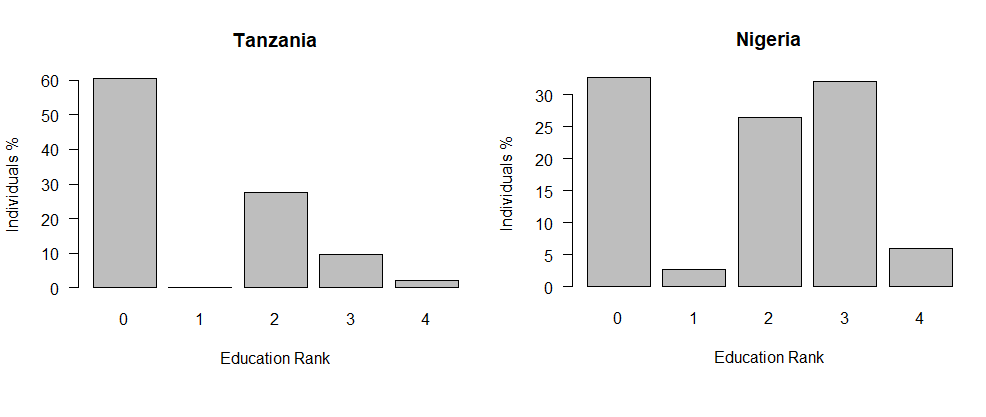
\includegraphics[width=6in]{subchapters/figures/tnz_ngr_educranks2014-2015}
\par\end{centering}
\caption{\label{fig:HistEducationRanks}Education ranks for populations in
Tanzania Nigeria (see Tables \ref{education_rank_tnz} and \ref{education_rank_ngr}
for rank classification)}
\end{figure}

\begin{figure}
\begin{centering}
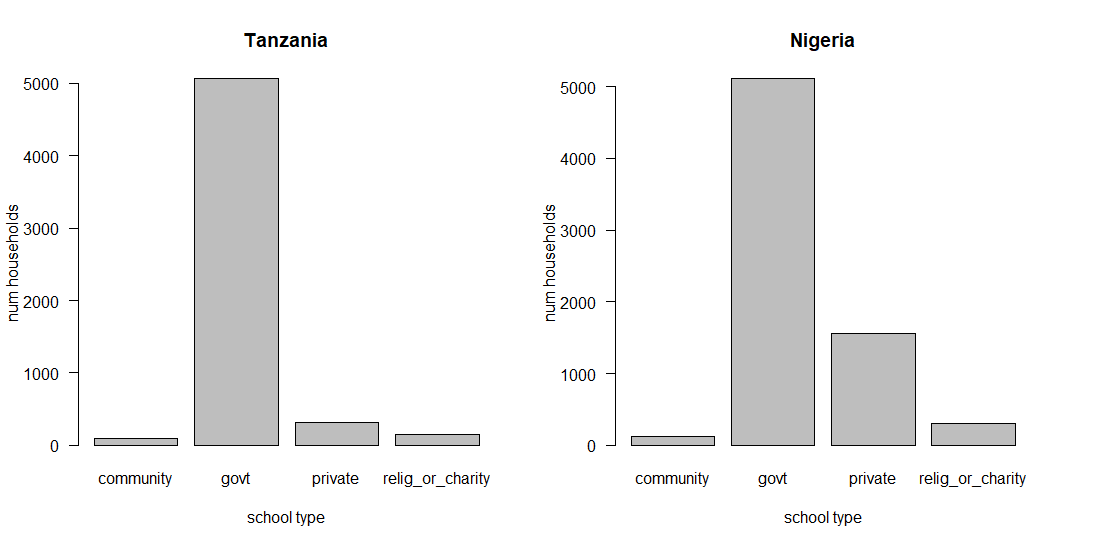
\includegraphics[width=6in]{subchapters/figures/tnz_ngr_schooltype2012}
\par\end{centering}
\caption{\label{fig:BarChartSchoolTypes}School types for non-adult population
in Tanzania and Nigeria}
\end{figure}

\begin{figure}
\begin{centering}
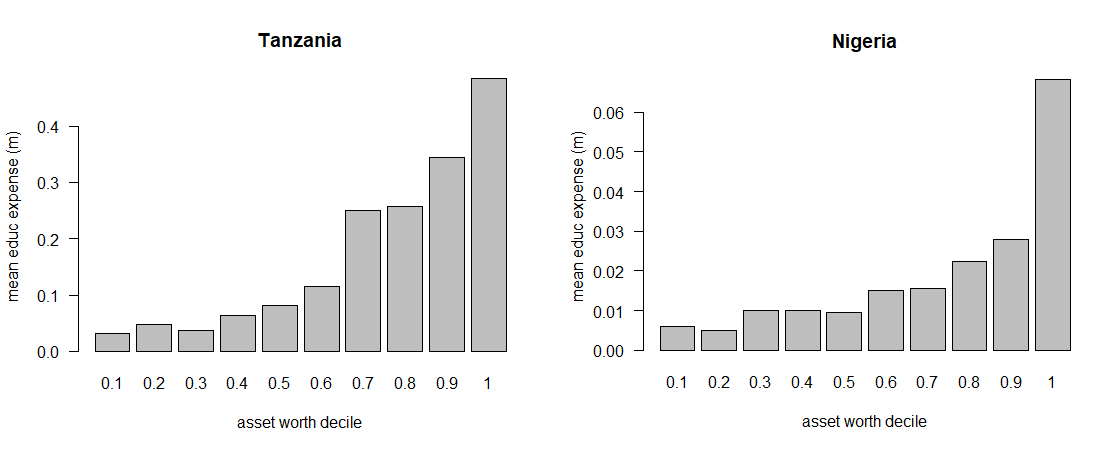
\includegraphics[width=6in]{subchapters/figures/tnz_ngr_toteducexpense2012}
\par\end{centering}
\caption{\label{fig:BarChartEducationbyAssetDeciles}Educational expenses averages
over deciles of asset worth in in Tanzania and Nigeria}
\end{figure}

% Getting rural vs urban average expenditures 
% ddply(tn$df2012 [,c("hhid2012","toteducexpense","isrural")],.(isrural),summarise,toteducexpense=mean(toteducexpense))
% Getting children's education-rank averages
% ced <- merge(unique(subset(o2012,age<18  & !is.na(highest_educ))[c("hhid","education_rank")]),unique(plyr::rename(tn$df2012,c("hhid2012"="hhid"))[,c("hhid","toteducexpense")]))
% ddply(ced,.(education_rank),summarise,toteducexpense2=mean(toteducexpense), n=length(toteducexpense))

\noindent

Considering the overall distribution of education expenses, we see
that the urban residents spend much higher on education than the rural
residents in both the economies. The urban residents spend 2.34 times
more than rural residents in Nigeria whereas they spend 2.8 times
more in Tanzania. The secondary education appears to get much costlier
in Tanzania since the mean education expenditure for tertiary education
(rank 3) is almost double that of the expenditure on secondary education
(rank 2) in Tanzania. In Nigeria, these expenditures rise by about
54\%. The educational expenses do not seem to rise much with asset
disparities in Nigeria - whereas they seem to be more unequally distributed
in Tanzania (see Figure \ref{fig:BarChartEducationbyAssetDeciles})\footnote{Despite the uniformity in LSMS data fields corresponding to education
expenses, the collection methodology may not be the same across all
the countries. This is evident from the much lower educational expenses
in Nigeria than in Tanzania (see Table \ref{tab:Summary-Stats}).
Our comparison of the two economies (Tanzania and Nigeria) therefore
does not rely on the measurement of educational expenses relative
to one another.}. Comparing education levels of the household heads, we see that the
average-education rank of the household heads in Tanzania (1.8) is
lower than that in Nigeria(1.9). We also see that the role of private
education is much higher in Nigeria (see Figure \ref{fig:BarChartSchoolTypes}).

\begin{table}[h] \centering

\resizebox{6in}{!}{
\begin{tabular}{>{\raggedright}p{1.4in}|>{\raggedleft}p{0.6in}|>{\raggedleft}p{.6in}|>{\raggedleft}p{.6in}|>{\raggedleft}p{0.6in}|>{\raggedleft}p{0.6in}|>{\raggedleft}p{0.6in}   } 

\tabularnewline            & \multicolumn{2}{c}{\emph{Tanzania}}  & &   \multicolumn{2}{c}{\emph{Nigeria}} \tabularnewline 
\hline  
Variable & $mean_{tnz}$   & $median_{tnz}$  & $stdev_{tnz}$    & $mean_{ngr}$ & $median_{ngr}$  & $stdev_{ngr}$ \tabularnewline \hline 
\texttt{w\_educ}  & 0.04 & 0.01 & 0.08 & 0.04 & 0 & 0.1 \tabularnewline \hline   
\texttt{log\_educ}   & 7.77 & 10.49 & 5.46 & 3.97 & 0 & 4.94 \tabularnewline \hline   
\texttt{\small{}ln\_tot\_exp} & 14.39 & 14.48 & 0.83 & 12.42 & 12.45 & 0.72\tabularnewline \hline  
\texttt{\small{}ln\_tot\_assets} & 12.96 & 12.76 & 1.93 & 10.93 & 11 & 1.35 \tabularnewline \hline  
\texttt{\small{}localwealth}     & 14.9 & 14.8 & 1.13 & 11.43 & 11.42 & 0.74 \tabularnewline \hline 
\texttt{\small{}localwealth\_educ} & 14.71 & 14.62 & 1.4 & 11.42 & 11.49 & 0.83 \tabularnewline \hline  
\texttt{\small{}localwealth\_agri} & 14.79 & 14.82 & 1.23 & 11.36 & 11.39 & 0.84 \tabularnewline \hline  
\texttt{\small{}log\_mean\_cost\_ne} & 12.9 & 12.97 & 0.53 & 10.85 & 10.86 & 0.53 \tabularnewline \hline   
\texttt{\small{}rural\_wards} & 0.66 & 0.78 & 0.33 & 0.71 & 1 & 0.41 \tabularnewline \hline   
\texttt{secondary\_schools} & 4.56 & 2 & 7.59 & 1.22 & 1 & 0.52 \tabularnewline \hline   
\texttt{educpriv} & 0.06 & 0 & 0.23 & 0.19 & 0 & 0.39 \tabularnewline \hline   
\texttt{is\_primaryage} & 0.63 & 1 & 0.48 & 0.76 & 1 & 0.43 \tabularnewline \hline   
\texttt{is\_secondaryage}  & 0.58 & 1 & 0.49 & 0.61 & 1 & 0.49 \tabularnewline \hline   
\texttt{is\_tertiaryage} & 0.45 & 0 & 0.5 & 0.4 & 0 & 0.49  \tabularnewline \hline   
\texttt{\small{}agri} & 0.66 & 1 & 0.47 & 0.51 & 1 & 0.5 \tabularnewline \hline   
\texttt{\small{}highesteduc } &1.21 & 1 & 1.06 & 1.53 & 2 & 1.47 \tabularnewline \hline   
\texttt{\small{}numchild} &3.05 & 3 & 2.03 & 3.55 & 3 & 2.16 \tabularnewline \hline   
\texttt{religion}  &  &  &  & 1.5 & 1 & 0.52 \tabularnewline \hline   
\texttt{has\_english}  & 0.36 & 0 & 0.48 &  &  &
\end{tabular} }
\caption{\label{tab:Summary-Stats}Summary Statistics for Variables in Tables \ref{tab:Dependent-Variables} and \ref{tab:Control-Variables}}
\end{table}

Using the average, median and standard deviation values variables
listed in Tables \ref{tab:Dependent-Variables} and \ref{tab:Control-Variables})
that are shown in Table \ref{tab:Summary-Stats}, we note that the
measures for average budget shares (\texttt{w\_educ}) as well as educational
expenses (\texttt{ln\_tot\_exp}) are not dissimilar in both the economies.
The average number of children in households that are of an age appropriate
for primary, secondary or tertiary education are not far from each
other either (see values for \texttt{is\_primaryage} , \texttt{is\_secondaryage}
and \texttt{is\_tertiaryage} in Table \ref{tab:Summary-Stats}). A
clear difference between Tanzania and Nigeria - however - is that
of standard-deviation in local wealth  (\texttt{localwealth}) - which
is higher for Tanzania. Further, the predominance of agricultural
occupations (see stdev values for \texttt{agri}) is higher for Tanzania
as well.

It is worth pointing that barring such broad observations, the LSMS
data used in our analyses may not permit a cross country comparison
for education expenses in a much finer detail. One reason is simply
that the distribution of savings, income and employment opportunities
may be too different in the two economies. The other reason is that
there is also a difference in sizes or granularity of district classifications
in the two economies. More specifically, the sizes of districts in
Tanzania seem much larger (particularly in the rural parts) than in
Nigeria. This is why the per-district density of secondary education
facilities - which we measure with the variable \texttt{secondary\_schools}
- is reported lower in Nigeria (see values corresponding to \texttt{secondary\_schools}
in Table \ref{tab:Summary-Stats}) - while the education levels of
the consumer populations remains higher in Nigeria (see highest\_educ
in Table \ref{tab:Summary-Stats}). The ruralness of districts - measured
as number of wards declared as rural in a district (i.e. the variable
\texttt{rural\_wards}) - does not seem affected by this disparity
in sizes as much (compare the values for \texttt{rural\_wards} in
Table \ref{tab:Summary-Stats}) - since a rural-urban classification
that declares boundaries of a district based on areas surrounding
an urban (or semi-urban) centre tends to bring a uniformity to the
number of rural wards in a district.

It is worth emphasising that the overall distribution of assets (durable
goods stocks) in the two countries is disparate - as is clear with
a direct comparison of asset values. Contrasting the Lorenz curves
for total non-durable expenditure and total assets in the Figure \ref{fig:LorenzCurves}
for in Nigeria and Tanzania, we note that distribution of assets is
more sparse in Tanzania even though the overall expenditure appears
similarly distributed in the two countries.

A geographical distribution of assets further details that higher-income
occupations are far fewer in the hinterland and the southern regions
of Tanzania (see Figure \ref{fig:occupations_r_tn-1} ) - relative
to the eastern and coastal regions that seem largely urban. The disparities
in occupations are less in Nigeria (see Figure \ref{fig:occupations_r_ngr}
).

\begin{figure}[h]
\begin{centering}
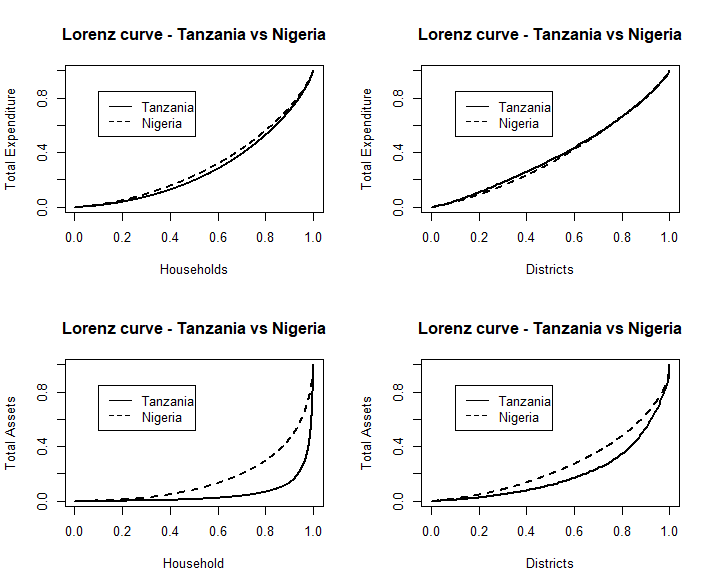
\includegraphics[width=6in]{subchapters/figures/tnz_ngr_lorenz_curves_assets_logx_district_individual}
\par\end{centering}
\caption{\label{fig:LorenzCurves}Inequality in assets and non-durable expenditure
across households and districts}
\end{figure}

\onecolumn

\begin{figure}[h]
\begin{centering}
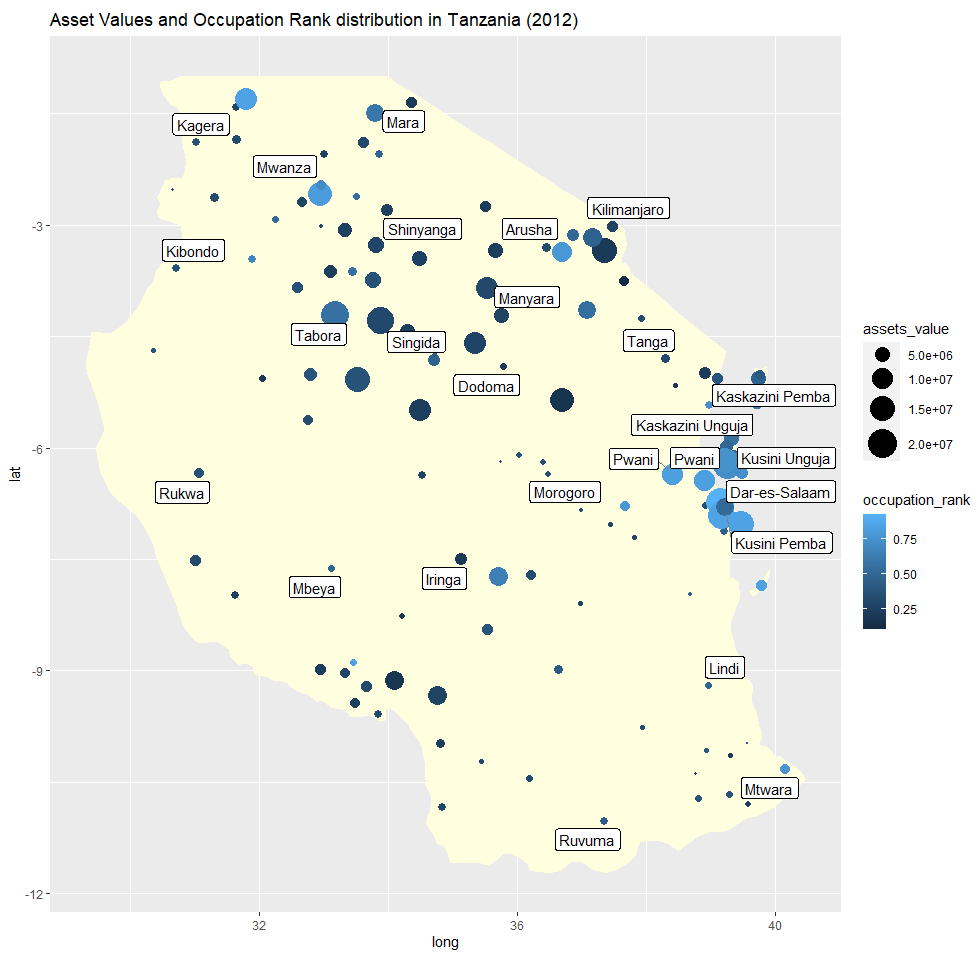
\includegraphics[width=5in]{subchapters/tnz_assets_occuprank_distribution_2012}
\par\end{centering}
\caption{\label{fig:occupations_r_tn-1}Occupations and consumer-owned assets
in Tanzania}
\end{figure}

\begin{figure}[h]
\begin{centering}
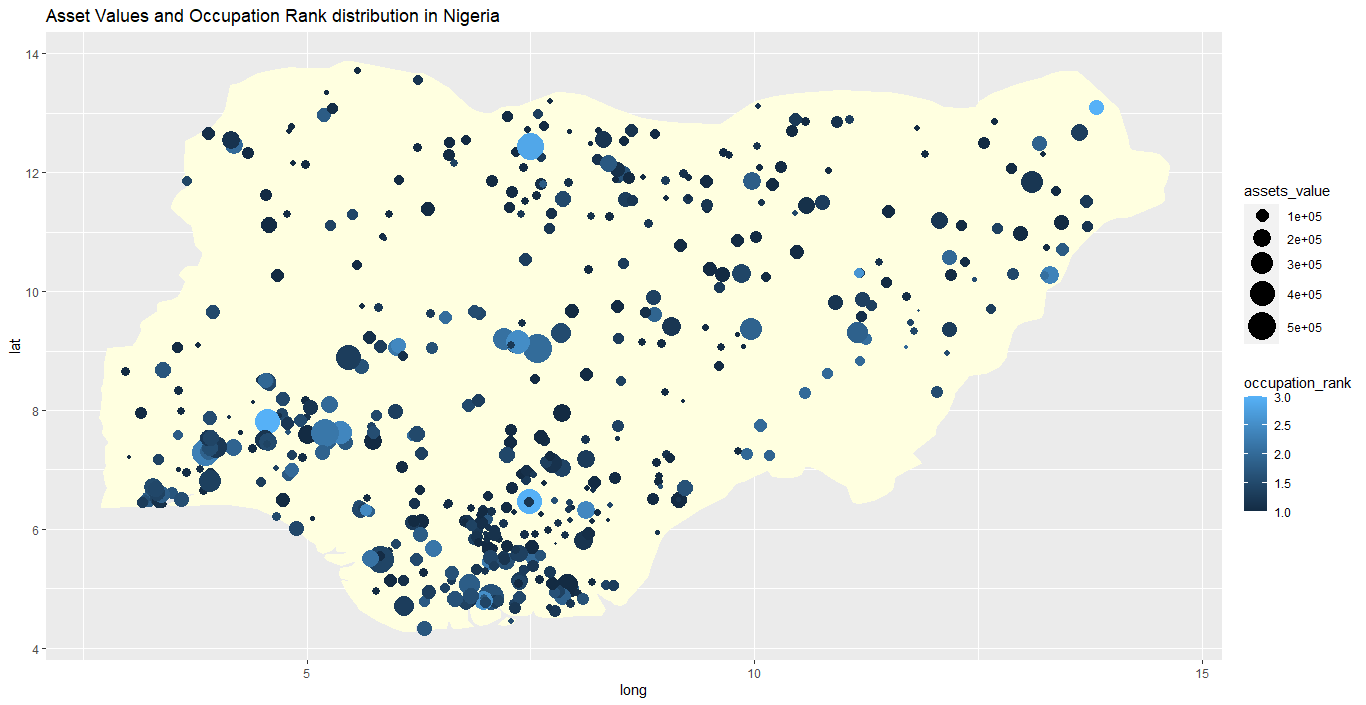
\includegraphics[width=6.5in]{subchapters/ngr_occup_2012}
\par\end{centering}
\caption{\label{fig:occupations_r_ngr}Occupations and consumer-owned assets
in Nigeria}
\end{figure}

Note that the occupation ranks shown in Figures \ref{fig:occupations_r_tn-1}
(Tanzania) and Figure \ref{fig:occupations_r_ngr} (Nigeria) are based
on the standardisation of various occupations in Tanzania and Nigeria.
Since the range of occupations in the surveys from Tanzania and Nigeria
is varied, the different occupations in the survey for Tanzania and
Nigeria have been standardised into occupation ranks (ranging from
0 to 3) based on the data on income derived from the occupations in
the survey so that a higher occupation rank represents an occupation
that provides higher income. The reason why the income itself is not
shown in the plots is that the data on income is far sparser than
the recall of assets and the reporting of occupations in surveys from
both the economies\footnote{It is not uncommon for the empirical studies in SSA to have the data
on occupation or education proxy the income differences \cite{AlesinaMobilityAfrica2019}.
The primary reason for this is the sparsity of income data - a problem
that may be further aggravated because of a large informal sectors
in the economies.}. The mapping from specific occupations to the occupation-ranks for
Tanzania and Nigeria is shown in Table \ref{occupation_rank_tn} and
\ref{occupation_rank_ngr} (respectively). A higher occupation rank
represents occupations that bring higher income. As described in Section
\ref{sec:Chapter2_Data}, the education levels are also mapped to
education ranks denoting primary, secondary and higher education (see
Table \ref{education_rank_tnz} for Tanzania and Table \ref{education_rank_ngr}
for Nigeria in the Appendix \ref{sec:education_1}). A higher education
rank corresponds to a higher education level.

While we undertake a more detailed view on education expenses in the
Section \ref{subsec:Results}, the key observation from the data is
that the disparities in income and durable goods are more localised
in Nigeria while they are more extreme across wider geographical regions
in Tanzania. More specifically, despite the southern areas of Nigeria
having more higher-paid occupations and a higher expenditure on non-durable
expenditure overall (see Figure \ref{fig:occupations_r_ngr}), the
disparity in durable-goods ownership across regions is not as extreme
as in Tanzania. The effect of this non-uniformity on consumption and
educational expenses is discussed in Section \ref{subsec:Results}.

% Lorenz curve plots
%plot(Lc(exp(ng$df2015$logx)))
% for individual totexp
%lorenz_curve(dat_a = exp(tn2012$logx),dat_b = exp(ng$df2012$logx),dat_a_name = "Tanzania",dat_b_name = "Nigeria",xlab = "Households",ylab = "Total Expenditure",use_cex = 1.)
% for district level totexp
%lorenz_curve(dat_a = exp(district_means(dat=tn2012,hhid_col = "hhid2012",field_type = "logx")$mean_logx),dat_b = exp(district_means(dat=ng$df2012,hhid_col = "hhid",field_type = "logx")$mean_logx),dat_a_name = "Tanzania",dat_b_name = "Nigeria",xlab = "Districts",ylab = "Total Expenditure",use_cex = 1.)
% for district level assets
%lorenz_curve(dat_a = exp(district_means(dat=tn2012,hhid_col = "hhid2012",field_type = "logA")$mean_logA),dat_b = exp(district_means(dat=ng$df2012,hhid_col = "hhid",field_type = "logA")$mean_logA),dat_a_name = "Tanzania",dat_b_name = "Nigeria",xlab = "Districts",ylab = "Total Assets",use_cex = 1.)
% For individual assets
%lorenz_curve(dat_a = exp(tn2012$logA),dat_b = exp(ng$df2012$logA),dat_a_name = "Tanzania",dat_b_name = "Nigeria",xlab = "Household",ylab = "Total Assets",use_cex = 1.)


\subsection{\label{subsec:Results}Results}

% We don't have panel information for 2012-2014 (for Tanzania). So we won't be using panel data. Pseudo-panel is a possibility but not considered.

\noindent

The two dependent variables we use in the estimation described in
Section \ref{sec:Econometric-Method} (see Equation \ref{eq:budgetshr_estimation})
are the budget shares for educational expenses (\texttt{$w_{educ}$})
and total expenditures (\texttt{$log(x_{educ})$}) . These dependent
variables are listed in Table \ref{tab:Dependent-Variables-1} while
controls used for the estimation are listed in Table \ref{tab:Control-Variables}.

%Variables : {wealth,wealth-conc/ruralwards,secondary_schools,occupation, parental education, language-religion, age, numchild, educpriv}

The two main explanatory variables used in the study are the logarithm
of total expenditure \texttt{ln\_tot\_exp} and the local wealth measure
\texttt{localwealth}. As discussed before, an alternative formulation
is also specified for comparison - where the two explanatory variables
are the logarithm of total assets value (\texttt{ln\_tot\_assets})
and the urban/rural indicators (\texttt{rural\_wards}). The physical
access to education (i.e. \texttt{secondary\_schools}) is an important
control in both the formulations. Other controls used in the comparison
are the indicator for an agrarian occupation \texttt{agri} ($\Omega$),
the paternal education level \texttt{highesteduc} ($\Gamma^{*}$),
the religion and language indicators ( \texttt{religion} $\chi$ used
only for Nigeria indicated by 1 for Christianity, 2 for Islam, 3 for
Traditional, 4 for other - and English-speaking ability i.e. the variable
\texttt{has\_english $\xi$ }indicating the ability to speak English
used only for Tanzania), the access to private education (\texttt{educpriv}
or $\pi$), the number of children ( \texttt{numchild} or $h$) and
their ages \texttt{is\_primaryage} ($\mu_{1}$),\texttt{ is\_secondaryage}
($\mu_{2}$)\texttt{, is\_tertiaryage} ($\mu_{3})$ indicating if
they are eligible (due to age) for primary, secondary or tertiary
education (respectively) and the non-durable consumption prices \texttt{\small{}(log\_mean\_cost\_ne}
$p_{ne}$). All of the controls remain the same for the main as well
as alternative formulation. Recall that the non-durable consumption
prices $p_{ne}$ (see Section \ref{sec:Chapter2_Data}) - interpreted
as the cost of living in the vicinity - is measured as \texttt{\small{}log\_mean\_cost\_ne}
- the logarithm of average consumption excluding the asset-related
costs in the consumer's vicinity. Notice that the factor variables
are prefixed with respective values \texttt{1.} , \texttt{2.} etc.
in the results.

Of the control variables and explanatory variables discussed above,
some are observed at the household level while others are observed
at the level of the consumer's district. The logarithm of total expenditure
\texttt{ln\_tot\_exp} and of the total assets-owned \texttt{ln\_tot\_assets}
are observed at the level of the household. Similarly, the agricultural-occupation
factor variable \texttt{agri} (indicating whether the household head
is employed in agriculture related occupation or not), the number
of children in the household \texttt{numchild}, the childrens' ages
factor variables \texttt{is\_primaryage} ,\texttt{ is\_secondaryage}
and \texttt{is\_tertiaryage} ), the private education factor variable
\texttt{educpriv}, the highest education rank \texttt{highesteduc}
corresponding to the paternal generations (father-relationship) in
a household, the ability to speak English \texttt{has\_english} (used
only for Tanzania) and the household religion \texttt{religion} (used
only for Nigeria) are all observed for a household. The variables
observed at the district (or 6-$km$ vicinity) are the number of wards
with an accessible (within 6-km distance) secondary-schools (\texttt{secondary\_schools}),
the rural wards (\texttt{\small{}rural\_wards}) in a district, the
respective measures of the local wealth\texttt{\small{} localwealth}
and the logarithm of the per-head cost non-durable consumption \texttt{\small{}log\_mean\_cost\_ne}
.

To reiterate, a significant number of household units in both the
economies are made up of joint families where the reported educational
expenses correspond to the grandchildren of the household head (HH).
The education level of the HH would thus point to the penultimate
generation for households where HH has grandchildren and the previous
generation for younger households where HH has young children. To
resolve this disparity, we avoid using the education rank of the HH
and instead use the highest education rank in the generation of the
students' parents \footnote{Only relations with the household head are reported in the survey.
Thus, there is no direct way of locating the parent of a child except
through the relation with the household-head.} \texttt{\small{}highesteduc} instead. The paternal educational level
\texttt{\small{}highesteduc} suffices for our analysis of expenditure
spent over all the children in the household (rather than how education
budget is distributed among the male/female children). As mentioned
in the Section \ref{sec:Econometric-Method}, the households with
no children are ignored in the analysis. Nearly 22\% of households
in the Nigeria and 15 \% of households in Tanzania are thus excluded
from our comparison.

Notice also that the age-variables \texttt{is\_primaryage}, \texttt{is\_secondaryage},
\texttt{is\_tertiaryage} for attendance of primary, secondary and
tertiary education have been used in the analysis to get around the
unavailability of the current-education level of the household member
in the Nigerian LSMS survey data. Instead, we use a combination of
the indicator variable telling whether a household member is in school
or not (available in the surveys for both Tanzania and Nigeria) and
the mean school attendance ages to define variables \texttt{is\_primaryage},
\texttt{is\_secondaryage} and \texttt{is\_tertiaryage} that indicate
whether there is a household member of an age appropriate for attending
primary, secondary and tertiary education levels (respectively).

% For Nigeria: length(unique(subset(ng$df2015,toteducexpense==0)$hhid))/length(unique(ng$df2015$hhid)) = .67493
% For Tanzania: length(unique(subset(tn$df2014,toteducexpense==0)$hhid))/length(unique(tn$df2014$hhid)) = .4215

The results from the a tobit estimation for educational expenses (\texttt{$w_{educ}$})
and total expenditures (\texttt{$log(x_{educ})$}) with local wealth\texttt{
localwealth} as one of the controls are shown in Table \ref{tabTNZNGR_r}
for both Tanzania and Nigeria. The tobit uses a lower limit of zero
given a number of houses have no expenditure on education. A zero
expenditure is reported for nearly 65\% households in the survey from
Nigeria (2015) and 43\% households in the survey from Tanzania (2014).
This suggests that either the education expenses are recorded in more
detail in Tanzania or that a certain basic level of expenses is not
considered in the survey for Nigeria. The particular disparity also
limits our ability to compare educational expenses relative to one
another for the two economies. A discussion on the cross-section results
from the latest available years 2014 for Tanzania and 2015 for Nigeria
follows in Section \ref{subsec:Discussion} (see Table \ref{tabTNZNGR_r}).
The results from the alternative formulation - where the main explanatory
variables are the logarithm of total assets value \texttt{\small{}ln\_tot\_assets}
(used in place of household total expenditure) and the ruralness-score
\texttt{\small{}rural\_wards }derived from the survey's classification
of rural and urban areas (used in place of local wealth \texttt{\small{}localwealth})
- are also discussed in \ref{subsec:Discussion} (see Table \ref{tabTNZNGR_urbanrural}).

\newpage

\subsection{\label{subsec:Discussion}Discussion}

%[secondary_schools effect]
%For Nigeria, the secondary-schools were split into community and government schools - whose sum turns out to be less than the schools recorded in the previous year. This seems to the cause of some disparity in the two years - even though the effect of this variable does not appear as significant as wealth.
% NGR:
% a<- merge(ddply(unique(subset(ng$df2012[,c("region","district","secondary_schools")],!is.na(secondary_schools))),.(region),summarise,n=sum(secondary_schools)), ddply(unique(subset(ng$df2015[,c("region","district","secondary_schools")],!is.na(secondary_schools))),.(region),summarise,n=sum(secondary_schools)), by =c("region"))
% b<- merge(ddply(unique(subset(tn$df2012[,c("region","district","secondary_schools")],!is.na(secondary_schools))),.(region),summarise,n=sum(secondary_schools)), ddply(unique(subset(tn$df2014[,c("region","district","secondary_schools")],!is.na(secondary_schools))),.(region),summarise,n=sum(secondary_schools)), by =c("region"))
%[secondary_schools effect]


\noindent

%[ln_tot_exp effect on budget share]

\subsubsection*{Results with \texttt{$w_{educ}$ }as the dependent variable}

\noindent

The coefficient of the total expenditure ( \texttt{ln\_tot\_exp)}
in Table \ref{tabTNZNGR_r} for $w_{educ}$ as the dependent variable
suggest that an increase in the total expenditure ( \texttt{ln\_tot\_exp)}
causes a decrease in the budget share on education \texttt{($w_{educ}$}
) for both Tanzania and Nigeria. This seems largely due to the educational
expenses forming a higher proportion of the total expenditure for
poorer households - since the education expenditures $log(x_{educ})$
do seem to rise with the increase in total expenditure ( \texttt{ln\_tot\_exp)}
in Tanzania (see coefficient of \texttt{ln\_tot\_exp} under columns
for $log(x_{educ})$ in Table \ref{tabTNZNGR_r} ). The effect of
non-durable consumption prices (\texttt{log\_mean\_cost\_ne} ) is
weak on education-budget share \texttt{$w_{educ}$} for both the economies
(see coefficient of \texttt{log\_mean\_cost\_ne} under $w_{educ}$
in Table \ref{tabTNZNGR_r}) . Thus while urban developments must
raise the prices of non-durable expenditure \texttt{log\_mean\_cost\_ne},
the disparity in budget shares does not appear to be due to higher
cost of living (non-durable consumption) alone. In other words, the
effect of lower or higher cost of living on education expenditure
is weak across the regions in both the economies.

%[r - w_educ]

Instead, we see a strong and positive effect of local wealth ( \texttt{localwealth}
) towards educational budget shares (\texttt{$w_{educ}$}) in both
the countries in Table \ref{tabTNZNGR_r} (see coefficients of \texttt{localwealth}
under $w_{educ}$ in Table \ref{tabTNZNGR_r} ). This is an indication
of the regional disparities in the economies. More particularly, the
differences in average assets accumulation indicate the local wealth
has a strong effect on education expenses - despite controlling for
the effect of physical access. While absence of educational facilities
must clearly suppress education expenses in a region, the positive
effect of local wealth after controlling for availability of education
facilities coul be due to certain environmental factors that contribute
to education - such as a competition towards higher income social
positions or presence of occupations requiring higher levels of education
- factors with an important role after the availability of educational
facilities has been considered.

The effects of household total expenditure remain relevant - however
- for private education - which is limited to the wealthier households
in both the economies regardless of local wealth ( \texttt{localwealth}
). While a higher proportion of young population seems to be in private
schools in Nigeria (see Figure \ref{fig:BarChartSchoolTypes}), private
education is slightly higher in budget share in Tanzania as the privately-educated
households in Nigeria show higher budget shares \texttt{$w_{educ}$
}(see coefficients of \texttt{educpriv} under $w_{educ}$ for the
two countries in Table \ref{tabTNZNGR_r} ). However, since private
education only accounts for a minority of the population in both the
economies (see Figure \ref{fig:BarChartSchoolTypes}), the role of
access to either or private or government secondary school i.e. we
focus on the variable \texttt{secondary\_schools} for our comparison
of education expenses in the two countries.

Viewing the effect of the variable \texttt{secondary\_schools} on
education budget shares \texttt{$w_{educ}$}, we see a far stronger
effect of \texttt{secondary\_schools} for Tanzania (compare the coefficients
for secondary-school $s$ i.e. \texttt{secondary\_schools }in Tables
\ref{tabTNZNGR_r}) . It also seems that the consumers are more likely
to spend on primary education in Tanzania - as the access to secondary
and tertiary-education remains much lower (this is further elaborated
in discussion below of the results using education expenditure \texttt{$log(x_{educ})$}
as dependent variable).

The results from the alternative formulation using urban-rural indicators
suggest a particular limitation of the use of urban-rural indicators
from the survey. More specifically, the coefficients of rural-wards
\texttt{(rural\_wards}) for education budget shares \texttt{$w_{educ}$}
are negative and significant for Tanzania in Table \ref{tabTNZNGR_urbanrural}.
However, the inference of a higher expenditure on education - when
using urban-rural indicators - by the rural residents in Nigeria (see
significance of rural-wards \texttt{rural\_wards }in Table \ref{tabTNZNGR_urbanrural}
) may be improper as it ignores the fact that the wards identified
as rural in Nigeria may not be as rural as those identified as rural
in Tanzania. This is confirmed with the weaker role of wealth i.e.
assets-worth-logarithm ( \texttt{ln\_tot\_assets} in Table \ref{tabTNZNGR_urbanrural})
and a strong role for local wealth (\texttt{localwealth} in Table
\ref{tabTNZNGR_r}) for Nigeria in the alternative formulation.

%[log(x_educ)]

\subsubsection*{Results with \texttt{$log(x_{educ})$ }as the dependent variable}

\noindent

Comparing the results with education-expenditure logarithm \texttt{$log(x_{educ})$
}as the dependent variable, we see that the education expenditures
rise with the increase in total expenditure logarithm (\texttt{ln\_tot\_exp})
for Tanzania but the effect of total expenditure \texttt{\small{}ln\_tot\_exp}
(in Table \ref{tabTNZNGR_r}) is not significant for Nigeria. While
the higher expenditure on education measured through total education
expenditure logarithm \texttt{$log(x_{educ})$} does seem to respond
to the prices of non-durable consumption \texttt{log\_mean\_cost\_ne}
in Tanzania (see coefficient of \texttt{log\_mean\_cost\_ne} under
column $log(x_{educ})$ in Table \ref{tabTNZNGR_r}), the effect of
non-durable consumption prices \texttt{log\_mean\_cost\_ne} remains
weak on education-budget share \texttt{$w_{educ}$} for both the economies
(see above discussion using budget share \texttt{$w_{educ}$} as the
dependent variable). We also see that the educational expenditure
$log(x_{educ})$ rises with the second explanatory variable i.e. the
local wealth ( \texttt{localwealth} ) for Nigeria while the effect
of local wealth \texttt{localwealth} is insignificant for Tanzania
(compare coefficients for \texttt{localwealth} against both the countries
in Table \ref{tabTNZNGR_r} under columns for $log(x_{educ})$ ).
In the alternative formulation where urbanisation is measured with
the ruralness score ( \texttt{rural\_wards} ), the ruralness score
corresponds to a rise in educational expenditure \texttt{$log(x_{educ})$}
for Nigeria and a drop in educational expenditure \texttt{$log(x_{educ})$
}for Tanzania (see coefficients for \texttt{rural\_wards} under columns
for \texttt{$log(x_{educ})$} in Table \ref{tabTNZNGR_urbanrural}).
The disparity in the role of \texttt{rural\_wards} is however also
due to differences in the extent to which density of educational institutions
depends on \texttt{rural\_wards} in the respective countries.

Continuing with the comparison of results with education-expenditure
$log(x_{educ})$ as the dependent variable, we see that private-education
indicator variable \texttt{educpriv} is insignificant for Nigeria
(see Table \ref{tabTNZNGR_r} ). The education expenses in Nigeria
therefore depend less often on whether education is provided through
private educational institutions or not. The results also indicate
lower attendance (based on age) to secondary and tertiary-education
in Tanzania (see coefficients of secondary-school-age\texttt{ is\_secondaryage}
and tertiary-school-age \texttt{is\_tertiaryage} in regression results
with education expenditure logarithm $log(x_{educ})$ as the dependent
variable in Table \ref{tabTNZNGR_r}). In the alternative formulation,
the results with education expenditure logarithm \texttt{$log(x_{educ})$
}as dependent variable in Tables \ref{tabTNZNGR_urbanrural} show
the role of secondary-school access \texttt{secondary\_schools} to
be stronger for Nigeria when taking wealth i.e. total assets-worth
logarithm \texttt{ln\_tot\_assets }into account. The permanent income
effect thus seems stronger than access in both the economies but is
weaker for Nigeria where the enrollment into secondary and tertiary
education is higher - regardless of the differences in long-term assets
(measured with logarithm of assets-worth \texttt{ln\_tot\_assets}).
The decomposed view of expenses on education in terms of secondary
and primary education level further clarifies this observation - reflecting
the far lower access to secondary education in Tanzania.

\subsubsection*{Other controls}

\noindent

The role of the number of children (\texttt{numchild}) also seems
stronger in Tanzania than in Nigeria - but the effect is likely due
the education expenses primarily driven by the primary education levels
in Tanzania (as well as a higher percentage of households reporting
no education expenditure in the survey from Nigeria). Another consequence
of most households spending on primary education alone is that the
agrarian households appear as spending higher on education after considering
the local wealth among households with the same educational-status.
The education expenditure is higher for agrarian households in Tanzania
after taking into account their poor educational status (see coefficients
of agrarian-occupation-indicator \texttt{1.is\_agri} in Table \ref{tabTNZNGR_r}
under column for the education-expenditure-logarithm \texttt{$log(x_{educ})$}
dependent variable).

The effects of permanent income in Tanzania overall seem stronger,
but they ought to be considered in light of the much lower expenditure
on secondary (and higher) education and higher disparity in asset-ownership
(even after taking into account the lower urbanisation levels) in
Tanzania. The significance of logarithm of assets-worth ( \texttt{ln\_tot\_assets
}in Table \ref{tabTNZNGR_urbanrural}) does indicate a general trend
where those with higher inter-generational wealth and in urban areas
(see significance of \texttt{ln\_tot\_assets }and \texttt{rural\_wards}
in Table \ref{tabTNZNGR_urbanrural} for Tanzania $log(x_{educ})$
as dependent variable) are far more likely to avail the education
facilities, but a higher dependence on industrial output in Nigeria
also seems to have contributed to a higher demand for secondary and
tertiary education in the economy overall ( compare with significance
of \texttt{ln\_tot\_assets }, \texttt{1.is\_secondaryage} and \texttt{rural\_wards}
in Table \ref{tabTNZNGR_urbanrural} for Nigeria with $log(x_{educ})$
as dependent variable). Another observation - the stronger role of
father's education level in Tanzania - also seems related with these
disparities in the two economies as well. A comparison of education
expenditures across the two countries must take into account the different
stages which the two countries appear to be in terms of urbanisation
and economic development.

Finally, the role of social environment is found significant in both
the economies. The role of English language seems significant in Tanzania
- where the English-speakers spend significantly higher on education
(see coefficients of \texttt{has\_english} in Table \ref{tabTNZNGR_r}
under  $log(x_{educ})$ )\textbf{ }. In Nigeria, on the other hand,
the educational expenses are higher among households identifying as
Christian (see coefficients of\texttt{ religion} in Table \ref{tabTNZNGR_r}
under $log(x_{educ})$ ) . In both cases, the role of social characteristics
may be rather inseparable from differences in educational institutions.
In case of Tanzania, the ability to speak English is aligned with
attending educational institutions while in Nigeria, the role played
by Christian missionaries in establishment of educational institutions
may be reflected in the disparity of access to educational facilities.

\begin{table}\centering
\caption{Tanzania -Nigeria - Differences in Local Wealth \label{tabTNZNGR_r}}
\resizebox{4in}{!}{
\def\sym#1{\ifmmode^{#1}\else\(^{#1}\)\fi}     
\begin{tabular} { l c c  c c }
\hline\hline       

          &\multicolumn{2}{c}{$w_{educ}$}       &\multicolumn{2}{c}{$log(x_{educ})$}  \\\cmidrule(lr){2-3}\cmidrule(lr){4-5}           &\multicolumn{1}{c}{}&\multicolumn{1}{c}{}&\multicolumn{1}{c}{}&\multicolumn{1}{c}{}\\           &\multicolumn{1}{c}{\emph{Tanzania}}&\multicolumn{1}{c}{\emph{Nigeria}}&\multicolumn{1}{c}{\emph{Tanzania}}&\multicolumn{1}{c}{\emph{Nigeria}}\\ \midrule ln\_tot\_exp      & -0.00908\sym{**} &  -0.0283\sym{***}&    1.224\sym{***}&    0.133         \\           &  (0.004)         &  (0.000)         &  (0.000)         &  (0.744)         \\ localwealth     &  0.00488\sym{*}  &   0.0299\sym{***}&  -0.0368         &    1.497\sym{***}\\           &  (0.015)         &  (0.000)         &  (0.758)         &  (0.000)         \\ log\_mean\_cost\_ne&   0.0490         &   0.0479         &    9.165\sym{*}  &   -0.155         \\           &  (0.467)         &  (0.672)         &  (0.023)         &  (0.981)         \\ 1.agri    &  0.00735         &  0.00990         &    0.953\sym{**} &    0.574         \\           &  (0.167)         &  (0.308)         &  (0.003)         &  (0.297)         \\ 1.educpriv&   0.0756\sym{***}&   0.0475\sym{***}&    2.890\sym{***}&    0.815         \\           &  (0.000)         &  (0.000)         &  (0.000)         &  (0.197)         \\ 1.highesteduc&   0.0109\sym{*}  &   0.0829         &    0.694\sym{*}  &    5.899         \\           &  (0.030)         &  (0.301)         &  (0.021)         &  (0.202)         \\ 2.highesteduc&  0.00432         &  0.00679         &    0.366         &    0.363         \\           &  (0.711)         &  (0.585)         &  (0.598)         &  (0.607)         \\ 3.highesteduc&  0.00457         & -0.00520         &    0.473         &   -0.528         \\           &  (0.519)         &  (0.627)         &  (0.263)         &  (0.381)         \\ 4.highesteduc&   0.0250\sym{*}  &   0.0120         &    1.465\sym{*}  &    0.183         \\           &  (0.011)         &  (0.506)         &  (0.013)         &  (0.859)         \\ secondary\_schools& -0.00138\sym{***}&  0.00738         & -0.00569         &    0.384         \\           &  (0.000)         &  (0.373)         &  (0.734)         &  (0.414)         \\ 1.is\_primaryage&   0.0793\sym{***}&   0.0538\sym{***}&    8.842\sym{***}&    3.301\sym{***}\\           &  (0.000)         &  (0.000)         &  (0.000)         &  (0.000)         \\ 1.is\_secondaryage&   0.0123\sym{**} &   0.0605\sym{***}&    0.143         &    2.230\sym{***}\\           &  (0.005)         &  (0.000)         &  (0.580)         &  (0.000)         \\ 1.is\_tertiaryage&  -0.0131\sym{**} &   0.0174         &   -1.281\sym{***}&    0.931         \\           &  (0.001)         &  (0.056)         &  (0.000)         &  (0.071)         \\ 1.has\_english&   0.0584\sym{***}&                  &    2.249\sym{***}&                  \\           &  (0.000)         &                  &  (0.000)         &                  \\ numchild  &  0.00433\sym{***}& -0.00221         &    0.259\sym{***}&  -0.0499         \\           &  (0.000)         &  (0.360)         &  (0.000)         &  (0.714)         \\ 2.religion&                  &  -0.0455\sym{***}&                  &   -2.043\sym{***}\\           &                  &  (0.000)         &                  &  (0.000)         \\ 3.religion&                  &  -0.0632         &                  &   -2.160         \\           &                  &  (0.170)         &                  &  (0.396)         \\ \_cons    &   -0.151         &   -0.231         &   -41.97\sym{***}&   -22.99         \\           &  (0.346)         &  (0.352)         &  (0.000)         &  (0.103)         \\ \midrule sigma     &                  &                  &                  &                  \\ \_cons    &   0.0876\sym{***}&    0.173\sym{***}&    5.361\sym{***}&    9.969\sym{***}\\           &  (0.000)         &  (0.000)         &  (0.000)         &  (0.000)         \\ \midrule \(N\)     &     2410         &     2192         &     2410         &     2192         \\ 

\end{tabular}
}
\end{table}

\begin{table}\centering
\caption{Tanzania-Nigeria - Urban-Rural Differences \label{tabTNZNGR_urbanrural}}
\resizebox{4in}{!}{
\def\sym#1{\ifmmode^{#1}\else\(^{#1}\)\fi}     
\begin{tabular} { l c c  c c }
\hline\hline       

          &\multicolumn{2}{c}{$w_{educ}$}       &\multicolumn{2}{c}{$log(x_{educ})$}  \\\cmidrule(lr){2-3}\cmidrule(lr){4-5}           &\multicolumn{1}{c}{}&\multicolumn{1}{c}{}&\multicolumn{1}{c}{}&\multicolumn{1}{c}{}\\           &\multicolumn{1}{c}{\emph{Tanzania}}&\multicolumn{1}{c}{\emph{Nigeria}}&\multicolumn{1}{c}{\emph{Tanzania}}&\multicolumn{1}{c}{\emph{Nigeria}}\\ \midrule ln\_tot\_assets      & -0.00590\sym{***}& -0.00196         &    0.392\sym{***}&    0.363         \\           &  (0.000)         &  (0.576)         &  (0.000)         &  (0.065)         \\ log\_mean\_cost\_ne&  -0.0548         & -0.00483         &    9.559\sym{*}  &    8.263         \\           &  (0.455)         &  (0.965)         &  (0.031)         &  (0.182)         \\ 1.agri    &   0.0106\sym{*}  &  0.00507         &    0.925\sym{**} &  -0.0768         \\           &  (0.048)         &  (0.617)         &  (0.004)         &  (0.892)         \\ 1.educpriv&   0.0800\sym{***}&   0.0506\sym{***}&    2.730\sym{***}&    1.016         \\           &  (0.000)         &  (0.000)         &  (0.000)         &  (0.113)         \\ 1.highesteduc&   0.0107\sym{*}  &   0.0948         &    0.679\sym{*}  &    7.172         \\           &  (0.032)         &  (0.244)         &  (0.023)         &  (0.121)         \\ 2.highesteduc&  0.00199         &  0.00689         &    0.512         &    0.481         \\           &  (0.864)         &  (0.583)         &  (0.462)         &  (0.495)         \\ 3.highesteduc&  0.00359         & -0.00767         &    0.607         &   -0.551         \\           &  (0.608)         &  (0.478)         &  (0.149)         &  (0.361)         \\ 4.highesteduc&   0.0273\sym{**} &   0.0129         &    1.320\sym{*}  &    0.486         \\           &  (0.005)         &  (0.480)         &  (0.025)         &  (0.636)         \\ secondary\_schools& -0.00111\sym{***}&   0.0147         &  0.00265         &    0.906         \\           &  (0.000)         &  (0.085)         &  (0.875)         &  (0.058)         \\ 1.is\_primaryage&   0.0797\sym{***}&   0.0562\sym{***}&    8.812\sym{***}&    3.408\sym{***}\\           &  (0.000)         &  (0.000)         &  (0.000)         &  (0.000)         \\ 1.is\_secondaryage&   0.0129\sym{**} &   0.0593\sym{***}&    0.145         &    2.259\sym{***}\\           &  (0.003)         &  (0.000)         &  (0.572)         &  (0.000)         \\ 1.is\_tertiaryage&  -0.0121\sym{**} &   0.0139         &   -1.240\sym{***}&    0.878         \\           &  (0.003)         &  (0.132)         &  (0.000)         &  (0.088)         \\ rural\_wards&  -0.0229\sym{**} &   0.0133         &   -1.184\sym{*}  &    1.848\sym{**} \\           &  (0.007)         &  (0.291)         &  (0.021)         &  (0.009)         \\ 1.has\_english&   0.0599\sym{***}&                  &    2.436\sym{***}&                  \\           &  (0.000)         &                  &  (0.000)         &                  \\ numchild  &  0.00426\sym{***}& -0.00354         &    0.304\sym{***}&  -0.0588         \\           &  (0.000)         &  (0.143)         &  (0.000)         &  (0.662)         \\ 2.religion&                  &  -0.0445\sym{***}&                  &   -1.716\sym{**} \\           &                  &  (0.000)         &                  &  (0.003)         \\ 3.religion&                  &  -0.0725         &                  &   -2.411         \\           &                  &  (0.120)         &                  &  (0.343)         \\ \_cons    &    0.143         &   -0.103         &   -30.47\sym{**} &   -29.99\sym{*}  \\           &  (0.452)         &  (0.698)         &  (0.008)         &  (0.044)         \\ \midrule sigma     &                  &                  &                  &                  \\ \_cons    &   0.0870\sym{***}&    0.175\sym{***}&    5.357\sym{***}&    9.994\sym{***}\\           &  (0.000)         &  (0.000)         &  (0.000)         &  (0.000)         \\ \midrule \(N\)     &     2410         &     2192         &     2410         &     2192         \\ 

\end{tabular}
}
\end{table}

\bigskip{}

\begin{landscape}
\begin{table}[!htpb]\centering
\caption{Tanzania-Nigeria - around median assets-value \label{tabTNZNGR_abovebelow_median}}
\resizebox{7.5in}{!}{
\def\sym#1{\ifmmode^{#1}\else\(^{#1}\)\fi}     
\begin{tabular} { l c c  c c c c c c }
\hline\hline       

          &\multicolumn{2}{c}{$w_{educ}$}&\multicolumn{2}{c}{$log(x_{educ})$}&\multicolumn{2}{c}{$w_{educ}$}&\multicolumn{2}{c}{$log(x_{educ})$}\\\cmidrule(lr){2-3}\cmidrule(lr){4-5}\cmidrule(lr){6-7}\cmidrule(lr){8-9}           &\multicolumn{1}{c}{Above Median }&\multicolumn{1}{c}{Above Median }&\multicolumn{1}{c}{Above Median }&\multicolumn{1}{c}{Above Median }&\multicolumn{1}{c}{Below Median }&\multicolumn{1}{c}{Below Median }&\multicolumn{1}{c}{Below Median }&\multicolumn{1}{c}{Below Median }
\\           &\multicolumn{1}{c}{\emph{Tanzania}}&\multicolumn{1}{c}{\emph{Nigeria}}&\multicolumn{1}{c}{\emph{Tanzania}}&\multicolumn{1}{c}{\emph{Nigeria}}&\multicolumn{1}{c}{\emph{Tanzania}}&\multicolumn{1}{c}{\emph{Nigeria}}&\multicolumn{1}{c}{\emph{Tanzania}}&\multicolumn{1}{c}{\emph{Nigeria}}
\\ \midrule ln\_tot\_exp      & -0.00338         &  -0.0168         &    0.783\sym{**} &    0.411         &  -0.0121\sym{**} &  -0.0458\sym{***}&    1.272\sym{***}&   -0.582         \\           &  (0.483)         &  (0.113)         &  (0.005)         &  (0.511)         &  (0.006)         &  (0.000)         &  (0.000)         &  (0.321)         \\ localwealth     &  0.00512         &   0.0321\sym{***}&   -0.160         &    1.818\sym{***}&  0.00592         &   0.0227\sym{*}  &  -0.0190         &    0.819         \\           &  (0.061)         &  (0.000)         &  (0.311)         &  (0.000)         &  (0.052)         &  (0.024)         &  (0.919)         &  (0.131)         \\ log\_mean\_cost\_ne&  -0.0900         & -0.00476         &    11.02         &   -6.579         &    0.165         &    0.100         &    7.127         &    5.568         \\           &  (0.363)         &  (0.976)         &  (0.056)         &  (0.479)         &  (0.080)         &  (0.539)         &  (0.219)         &  (0.528)         \\ 1.agri    &  0.00286         &  0.00554         &    0.758         &    0.341         &   0.0129         &   0.0157         &    1.151\sym{*}  &    0.809         \\           &  (0.671)         &  (0.665)         &  (0.052)         &  (0.650)         &  (0.139)         &  (0.294)         &  (0.031)         &  (0.314)         \\ 1.educpriv&   0.0850\sym{***}&   0.0348\sym{*}  &    3.219\sym{***}&    0.726         &   0.0527\sym{**} &   0.0711\sym{***}&    2.083         &    0.896         \\           &  (0.000)         &  (0.010)         &  (0.000)         &  (0.364)         &  (0.004)         &  (0.000)         &  (0.074)         &  (0.406)         \\ 1.highesteduc&   0.0102         &   0.0847         &    0.443         &    8.091         &   0.0118         &    0.107         &    0.850\sym{*}  &    5.336         \\           &  (0.156)         &  (0.482)         &  (0.292)         &  (0.263)         &  (0.089)         &  (0.323)         &  (0.047)         &  (0.368)         \\ 2.highesteduc&   0.0208         &  0.00761         &    0.759         &    0.178         &  -0.0235         &  0.00660         &   -0.380         &    0.618         \\           &  (0.170)         &  (0.645)         &  (0.390)         &  (0.855)         &  (0.207)         &  (0.727)         &  (0.735)         &  (0.543)         \\ 3.highesteduc&-0.000380         & -0.00517         &  -0.0789         &   -0.359         &   0.0114         & -0.00197         &    1.171         &   -0.594         \\           &  (0.967)         &  (0.711)         &  (0.882)         &  (0.661)         &  (0.310)         &  (0.906)         &  (0.092)         &  (0.508)         \\ 4.highesteduc&   0.0204         &  0.00328         &    0.796         &   -0.695         &   0.0368         &   0.0426         &    2.572\sym{*}  &    2.785         \\           &  (0.079)         &  (0.877)         &  (0.240)         &  (0.577)         &  (0.062)         &  (0.222)         &  (0.036)         &  (0.139)         \\ secondary\_schools& -0.00128\sym{***}& -0.00325         & -0.00576         &   -0.524         & -0.00161\sym{**} &   0.0230         &  0.00286         &    1.669\sym{*}  \\           &  (0.000)         &  (0.764)         &  (0.770)         &  (0.413)         &  (0.001)         &  (0.077)         &  (0.926)         &  (0.018)         \\ 1.is\_primaryage&   0.0610\sym{***}&   0.0465\sym{**} &    7.280\sym{***}&    2.766\sym{**} &    0.101\sym{***}&   0.0664\sym{***}&    10.53\sym{***}&    3.983\sym{***}\\           &  (0.000)         &  (0.003)         &  (0.000)         &  (0.003)         &  (0.000)         &  (0.000)         &  (0.000)         &  (0.000)         \\ 1.is\_secondaryage&  0.00978         &   0.0692\sym{***}&   0.0488         &    2.637\sym{***}&   0.0161\sym{*}  &   0.0502\sym{***}&    0.243         &    1.706\sym{*}  \\           &  (0.100)         &  (0.000)         &  (0.887)         &  (0.000)         &  (0.011)         &  (0.000)         &  (0.533)         &  (0.020)         \\ 1.is\_tertiaryage&  -0.0109\sym{*}  &   0.0152         &   -1.381\sym{***}&    0.727         &  -0.0151\sym{*}  &   0.0193         &   -1.311\sym{***}&    1.108         \\           &  (0.043)         &  (0.197)         &  (0.000)         &  (0.292)         &  (0.015)         &  (0.181)         &  (0.001)         &  (0.152)         \\ 1.has\_english&   0.0496\sym{***}&                  &    1.789\sym{***}&                  &   0.0704\sym{***}&                  &    2.575\sym{***}&                  \\           &  (0.000)         &                  &  (0.000)         &                  &  (0.000)         &                  &  (0.000)         &                  \\ numchild  &  0.00204         & -0.00315         &    0.267\sym{**} &   -0.115         &  0.00657\sym{***}& -0.00143         &    0.231\sym{*}  &   0.0342         \\           &  (0.167)         &  (0.307)         &  (0.002)         &  (0.523)         &  (0.000)         &  (0.713)         &  (0.027)         &  (0.870)         \\ 2.religion&                  &  -0.0439\sym{***}&                  &   -1.963\sym{*}  &                  &  -0.0466\sym{**} &                  &   -2.037\sym{*}  \\           &                  &  (0.001)         &                  &  (0.011)         &                  &  (0.003)         &                  &  (0.015)         \\ 3.religion&                  &   -0.121         &                  &   -6.104         &                  &  -0.0373         &                  &   -0.447         \\           &                  &  (0.144)         &                  &  (0.192)         &                  &  (0.516)         &                  &  (0.882)         \\ \_cons    &    0.145         &   -0.250         &   -36.11\sym{**} &   -13.01         &   -0.447         &   -0.103         &   -39.80\sym{**} &   -22.74         \\           &  (0.521)         &  (0.475)         &  (0.006)         &  (0.527)         &  (0.061)         &  (0.777)         &  (0.007)         &  (0.246)         \\ \midrule sigma     &                  &                  &                  &                  &                  &                  &                  &                  \\ \_cons    &   0.0861\sym{***}&    0.169\sym{***}&    5.114\sym{***}&    10.13\sym{***}&   0.0877\sym{***}&    0.176\sym{***}&    5.545\sym{***}&    9.644\sym{***}\\           &  (0.000)         &  (0.000)         &  (0.000)         &  (0.000)         &  (0.000)         &  (0.000)         &  (0.000)         &  (0.000)         \\ \midrule \(N\)     &     1233         &     1192         &     1233         &     1192         &     1177         &     1000         &     1177         &     1000         \\ 

\end{tabular}
}
\end{table}
\end{landscape} 

\noindent

\subsection{Robustness Checks}

\subsubsection*{Assets ownership in poorer and richer sub-samples}

\noindent

To confirm that the assets-ownership does influence the access to
education, we inspect the role of assets in lower and higher sub-samples
of the surveyed population. We thus re-estimate the results with local
wealth \texttt{localwealth} as the explanatory variable for those
with less than the local median wealth i.e. assets-worth logarithm
\texttt{ln\_tot\_assets} and for those above it. The results demonstrate
how the education expenditures (coefficients for education budget-shares
\texttt{$w_{educ}$ }and education-expenditure logarithm \texttt{$log(x_{educ})$})
differ between the poorer and richer households in a given locality.
The results for above and below local median-assets possession using
education budget-shares \texttt{$w_{educ}$ }and education-expenditure-logarithm
\texttt{$log(x_{educ})$ }as the dependent variables are shown in
Table \ref{tabTNZNGR_abovebelow_median} for both above and below
median assets-possession levels in the two countries. 

%[Results from first robustness check ] social factors and secondary_schools . educpriv expected. tertiary_school level lower. num_child more nuanced - as is r. highesteduc also different.

While the role that the local wealth\texttt{ localwealth} plays towards
access to education appears similar for the rich and poor halves in
a locality as well, we do see a higher economic significance of local
wealth\texttt{ localwealth} for the below-median-assets household
in Nigeria - possibly because of high education costs in urban areas
where asset-possession may be lower. The access to private education
seems more widerspread in Nigeria as the below-median households seem
spend a higher budget-share on private-education. In Tanzania, on
the other hand, the economic significance of private-education factor
variable \texttt{educpriv }(as well as tertiary level education )
is higher for above-median households. The significance of social
factors - on the other hand - remains unaffected by whether the consumers
have above or below the median asset ownership level. More specifically,
the factor variables for English-speaking ability \texttt{has\_english}
and (i.e. \texttt{religion }) are significant in results from Tanzania
and Nigeria (respectively) for both richer and poorer households.
The factor variable for English-speaking ability \texttt{has\_english}
is significant for consumers both above and below media asset possession
level (the coefficient for variable \texttt{religion }is significant
for Nigeria for above and below median asset possession level in Table
\ref{tabTNZNGR_abovebelow_median}). The effect of secondary-schools
\texttt{secondary\_schools} is also the same for both richer and poorer
halves of a given locality. 

% It is worth pointing out that the economic significance for religion ( religion ) in Nigeria is higher with log(x_{educ}) as dependent variable in Table \ref{tabTNZNGR_abovebelow_median}. 


\begin{table}[!htpb] \centering

\resizebox{5in}{!}{

\begin{tabular}{>{\raggedright}p{.5in}|>{\raggedright}p{1.45in}|>{\centering}p{2in}|>{\centering}p{1.2in}} 
\hline  Variable  & Variable Name & Description & Additional Controls\tabularnewline 
\hline  $r$ & \texttt{localwealth} & Average over geographical vicinity (district) & $\Omega$ , education-rank\tabularnewline 
\hline  $r_{\Gamma}$ & \texttt{localwealth\_educ} & Separate averages over $\Gamma$ & $\Omega$\tabularnewline 
\hline  $r_{\Omega}$ & \texttt{localwealth\_agri} & Separate averages over $\Omega$ & education-rank\tabularnewline 
\end{tabular} 

}
\caption{\label{tab:ReferenceDefinitions}Prosperity levels and control variables used} 
\end{table}

\begin{table}[!htbp]\centering
\caption{Tanzania-Nigeria - $localwealth_{educ}$ \label{tabTNZNGR_reduc}}
\resizebox{4in}{!}{
\def\sym#1{\ifmmode^{#1}\else\(^{#1}\)\fi}     
\begin{tabular} { l c c  c c }
\hline\hline
 

          &\multicolumn{2}{c}{$w_{educ}$}       &\multicolumn{2}{c}{$log(x_{educ})$}  \\\cmidrule(lr){2-3}\cmidrule(lr){4-5}           &\multicolumn{1}{c}{  \emph{Tanzania}}&\multicolumn{1}{c}{\emph{Nigeria}}&\multicolumn{1}{c}{\emph{Tanzania}}&\multicolumn{1}{c}{\emph{Nigeria}}\\
\midrule ln\_tot\_exp      & -0.00927\sym{**} &  -0.0291\sym{***}&    1.229\sym{***}&   0.0988         \\           &  (0.004)         &  (0.000)         &  (0.000)         &  (0.809)         \\ localwealth\_educ &  0.00262         &   0.0272\sym{***}&  -0.0349         &    1.323\sym{***}\\           &  (0.102)         &  (0.000)         &  (0.714)         &  (0.000)         \\ log\_mean\_cost\_ne&   0.0535         &   0.0570         &    9.210\sym{*}  &    0.361         \\           &  (0.428)         &  (0.614)         &  (0.022)         &  (0.955)         \\ 1.agri    &  0.00598         &  0.00747         &    0.957\sym{**} &    0.449         \\           &  (0.256)         &  (0.440)         &  (0.002)         &  (0.412)         \\ 1.educpriv&   0.0763\sym{***}&   0.0471\sym{***}&    2.887\sym{***}&    0.799         \\           &  (0.000)         &  (0.000)         &  (0.000)         &  (0.207)         \\ 1.highesteduc&   0.0109\sym{*}  &   0.0819         &    0.697\sym{*}  &    5.867         \\           &  (0.031)         &  (0.307)         &  (0.020)         &  (0.204)         \\ 2.highesteduc&  0.00402         &  0.00520         &    0.369         &    0.285         \\           &  (0.731)         &  (0.676)         &  (0.595)         &  (0.687)         \\ 3.highesteduc&  0.00452         & -0.00734         &    0.475         &   -0.635         \\           &  (0.524)         &  (0.492)         &  (0.261)         &  (0.293)         \\ 4.highesteduc&   0.0250\sym{*}  &   0.0105         &    1.469\sym{*}  &    0.111         \\           &  (0.011)         &  (0.563)         &  (0.013)         &  (0.914)         \\ secondary\_schools& -0.00133\sym{***}&  0.00756         & -0.00571         &    0.400         \\           &  (0.000)         &  (0.361)         &  (0.732)         &  (0.395)         \\ 1.is\_primaryage&   0.0791\sym{***}&   0.0529\sym{***}&    8.844\sym{***}&    3.258\sym{***}\\           &  (0.000)         &  (0.000)         &  (0.000)         &  (0.000)         \\ 1.is\_secondaryage&   0.0119\sym{**} &   0.0599\sym{***}&    0.148         &    2.199\sym{***}\\           &  (0.006)         &  (0.000)         &  (0.566)         &  (0.000)         \\ 1.is\_tertiaryage&  -0.0133\sym{**} &   0.0177         &   -1.276\sym{***}&    0.950         \\           &  (0.001)         &  (0.051)         &  (0.000)         &  (0.065)         \\ 1.has\_english&   0.0579\sym{***}&                  &    2.253\sym{***}&                  \\           &  (0.000)         &                  &  (0.000)         &                  \\ numchild  &  0.00432\sym{***}& -0.00231         &    0.260\sym{***}&  -0.0547         \\           &  (0.000)         &  (0.337)         &  (0.000)         &  (0.687)         \\ 2.religion&                  &  -0.0441\sym{***}&                  &   -1.971\sym{***}\\           &                  &  (0.000)         &                  &  (0.001)         \\ 3.religion&                  &  -0.0609         &                  &   -2.074         \\           &                  &  (0.185)         &                  &  (0.414)         \\ \_cons    &   -0.124         &   -0.208         &   -42.21\sym{***}&   -21.67         \\           &  (0.438)         &  (0.401)         &  (0.000)         &  (0.124)         \\ \midrule sigma     &                  &                  &                  &                  \\ \_cons    &   0.0877\sym{***}&    0.173\sym{***}&    5.361\sym{***}&    9.974\sym{***}\\           &  (0.000)         &  (0.000)         &  (0.000)         &  (0.000)         \\ \midrule \(N\)     &     2410         &     2192         &     2410         &     2192         \\ 

\end{tabular}
}
\end{table}

\begin{table}\centering
\caption{Tanzania-Nigeria - $localwealth_{occup}$ \label{tabTNZNGR_roccup}}
\resizebox{4in}{!}{
\def\sym#1{\ifmmode^{#1}\else\(^{#1}\)\fi}     
\begin{tabular} { l c c  c c }
\hline\hline       

          &\multicolumn{2}{c}{$w_{educ}$}       &\multicolumn{2}{c}{$log(x_{educ})$}  \\\cmidrule(lr){2-3}\cmidrule(lr){4-5}           &\multicolumn{1}{c}{\emph{Tanzania}}&\multicolumn{1}{c}{\emph{Nigeria}}&\multicolumn{1}{c}{\emph{Tanzania}}&\multicolumn{1}{c}{\emph{Nigeria}}\\ \midrule ln\_tot\_exp      & -0.00924\sym{**} &  -0.0308\sym{***}&    1.147\sym{***}&  0.00661         \\           &  (0.003)         &  (0.000)         &  (0.000)         &  (0.987)         \\ localwealth\_agri&  0.00322         &   0.0276\sym{***}& -0.00759         &    1.352\sym{***}\\           &  (0.066)         &  (0.000)         &  (0.942)         &  (0.000)         \\ log\_mean\_cost\_ne&   0.0225         &   0.0496         &    3.952         &   -0.206         \\           &  (0.718)         &  (0.654)         &  (0.287)         &  (0.974)         \\ 1.educpriv&   0.0761\sym{***}&   0.0449\sym{***}&    2.930\sym{***}&    0.677         \\           &  (0.000)         &  (0.000)         &  (0.000)         &  (0.281)         \\ 1.highesteduc&   0.0109\sym{*}  &   0.0882         &    0.670\sym{*}  &    6.186         \\           &  (0.029)         &  (0.273)         &  (0.025)         &  (0.182)         \\ 2.highesteduc&  0.00401         &  0.00573         &    0.320         &    0.310         \\           &  (0.732)         &  (0.644)         &  (0.646)         &  (0.660)         \\ 3.highesteduc&  0.00444         & -0.00658         &    0.433         &   -0.603         \\           &  (0.531)         &  (0.535)         &  (0.306)         &  (0.314)         \\ 4.highesteduc&   0.0250\sym{*}  &   0.0104         &    1.382\sym{*}  &   0.0953         \\           &  (0.011)         &  (0.563)         &  (0.019)         &  (0.926)         \\ secondary\_schools& -0.00138\sym{***}&  0.00712         &  -0.0110         &    0.374         \\           &  (0.000)         &  (0.389)         &  (0.514)         &  (0.425)         \\ 1.is\_primaryage&   0.0794\sym{***}&   0.0542\sym{***}&    8.922\sym{***}&    3.328\sym{***}\\           &  (0.000)         &  (0.000)         &  (0.000)         &  (0.000)         \\ 1.is\_secondaryage&   0.0124\sym{**} &   0.0621\sym{***}&    0.168         &    2.314\sym{***}\\           &  (0.004)         &  (0.000)         &  (0.516)         &  (0.000)         \\ 1.is\_tertiaryage&  -0.0130\sym{**} &   0.0179\sym{*}  &   -1.287\sym{***}&    0.968         \\           &  (0.001)         &  (0.048)         &  (0.000)         &  (0.059)         \\ 1.has\_english&   0.0585\sym{***}&                  &    2.294\sym{***}&                  \\           &  (0.000)         &                  &  (0.000)         &                  \\ numchild  &  0.00444\sym{***}& -0.00169         &    0.279\sym{***}&  -0.0231         \\           &  (0.000)         &  (0.479)         &  (0.000)         &  (0.864)         \\ 2.religion&                  &  -0.0456\sym{***}&                  &   -2.063\sym{***}\\           &                  &  (0.000)         &                  &  (0.000)         \\ 3.religion&                  &  -0.0641         &                  &   -2.216         \\           &                  &  (0.163)         &                  &  (0.383)         \\ \_cons    &  -0.0517         &   -0.172         &   -27.46\sym{***}&   -19.34         \\           &  (0.711)         &  (0.469)         &  (0.001)         &  (0.153)         \\ \midrule sigma     &                  &                  &                  &                  \\ \_cons    &   0.0877\sym{***}&    0.173\sym{***}&    5.372\sym{***}&    9.965\sym{***}\\           &  (0.000)         &  (0.000)         &  (0.000)         &  (0.000)         \\ \midrule \(N\)     &     2410         &     2192         &     2410         &     2192         \\ 

\end{tabular}
}
\end{table}

\subsubsection*{Asset-density interpretations based on similar neighbours}

\noindent

To ensure that the effect of assets remains strong after accounting
for occupation or education level, we recompute the local wealth by
considering only those in the household's vicinity with the same value
of the indicator for primary/higher-than-primary education-level of
the household-head and then again with the same value for the agrarian/non-agrarian
occupation indicator. Three types of vicinities thus implied - are
summarised in Table \ref{tab:ReferenceDefinitions}. The first interpretation
is one that we have already described in Section \ref{subsec:Discussion}
- where a simple average of the total assets owned by the households
in the consumer's district is used. Both education rank and an agrarian-occupation
factor variable $\Omega$ indicating whether the household head's
occupation is agrarian or not are used as controls in this interpretation
of the vicinity. The second interpretation of the vicinity presented
as $r_{educ}$ in Table \ref{tabTNZNGR_reduc} is based on a supra-primary
factor variable $\Gamma$ indicating whether the education level of
the household-head is higher than primary school or not. More specifically,
this second interpretation uses the prosperity within the educational
levels implied by supra-primary factor variable $\Gamma$ (i.e. primary
and higher-than primary educational levels). The agrarian/non-agrarian
factor variable $\Omega$ is also used as the additional control in
this second interpretation. Finally, the third interpretation of vicinity
is based on the average prosperity in the agrarian vs non-agrarian
occupations (i.e. $\Omega$) and uses educational rank as the additional
control variable. The results from this third interpretation of vicinity
are presented in Table \ref{tabTNZNGR_roccup}.

Observing the differences in coefficients for local wealth calculated
over a supra-primary education vicinity ( \texttt{localwealth\_educ
}) and over agrarian/non-agrarian vicinity ( \texttt{localwealth\_agri}
) in Tables \ref{tabTNZNGR_reduc} and \ref{tabTNZNGR_roccup} (respectively)
for Tanzania and Nigeria, we see again that while the local wealth
corresponds to a rise in educational expenditure logarithm $log(x_{educ})$
for Nigeria, its effect is insignificant (whether one uses the local
wealth in the supra-primary-educated neighbourhood \texttt{localwealth\_educ
}or local wealth in the agrarian-neighbourhood \texttt{localwealth\_agri}
) for Tanzania. Further, since the coefficients for secondary-age
indicator \texttt{is\_secondaryage} seem higher for the agrarian/non-agrarian
vicinity (i.e. the coefficient for local wealth in \texttt{localwealth\_agri})
than for the supra-primary education vicinity ( i.e.\texttt{ }local
wealth in \texttt{localwealth\_educ}), it can be argued that education
expenses are more often clustered by agrarian or non-agrarian occupations
than by education levels the populations have attained.

\newpage

\section{\label{sec:Conclusions}Conclusions}

\noindent

We had set ourselves to examine the extent to which educational expenses
are influenced by local wealth and household permanent income in Nigeria
and Tanzania. While there are idiosyncratic differences between the
two countries we've used for our comparison, the weakening of effects
of permanent income within high local wealth areas is a notable implication
relevant to both the concerns for aspiration consumption and those
of education policy in the region.

Since the agrarian consumers maintain a high budget share on education
expenses in the poorer economy (Tanzania) and since higher education
ranks correspond to higher education expenses in the more developed
economy (Nigeria), one can argue that the educational expenses are
likely to remain high as more of the population attains education
as the regional prosperity rises. This also seems aligned with the
recent finding from a cohort-study by \citeA{porzio2021human} that
the labour with skills added through education is less willing to
stay in agricultural activities.

There are two main findings therefore that can be highlighted from
the results in the chapter. First, the effects of local wealth are
significant on education expenses in both the economies. Second, the
lower wealth continues to prevent access to education and mobility
in both the economies - even though rises in education expenses seem
inevitable when the employment opportunities increase in an economy.
In light of both the findings, the effects of permanent income as
well as wealth-effects appear less extreme in the higher developed
economy (i.e. Nigeria) than in the less developed economy (i.e. Tanzania).
One can thus argue that the effects of permanent income appear to
become weaker with rise in urban and economic development in the region.
Considered as aspirational consumption, the educational expenses may
thus continue to rise in the region with more local wealth accumulation.
Such a rise associated with weaker effects of permanent income supports
a view of conventional pathways to equity in both income and equality
\cite{KuznetsEconomicGrowthIneq2019}. Based on the arguments from
the first chapter, both participation costs and income inequality
may drive such changes.

From the view of education policy, the rise of education as a common
need does not discount the need to improve access to education for
the lower and middle-income populations in the region. While the literature
notes a higher significance of wealth effects, the consideration of
local wealth suggests that role of physical access may continue to
be important in economies with wide disparities in urban development.
This is of crucial importance also because the private educational
institutions - which are more common in Nigeria - do not yet play
a major role in the provision of education in the region. Instead,
a more significant role continues to be played by the state-institutions
in both the economies. The role of social differences indicated by
the significance of social characteristics in education expenses for
both the economies - further emphasises the need to improve wider
access to education. These findings seem aligned with the wider observations
made by \citeA{AlesinaMobilityAfrica2019} who elaborate on the significant
role of religious and colonial institutions in the educational mobility
across sub-Saharan Africa.

%[Different levels]

In summary, the development of the education sectors seems to be at
different stages of development in the Tanzania and Nigeria. The privatisation
of education in Nigeria seems to have coincided with attendance of
higher level education in a way that is yet to be seen for Tanzania
- where education has not expanded as much yet. The effects of permanent
income do seem strong in both the economies, but the relevance of
local wealth in the population having higher education levels points
to a promising albeit precarious direction where more urban developments
could improve access to education and employment opportunities in
the region while increasing expenses on education overall. Unlike
the typical high quality consumption, therefore, the education expenses
may continue to evolve - subject to participation costs and inequalities
- as a an expensive common need for the masses.

\newpage
\section{Appendices}
\subsection{Education and Occupation mappings}\label{sec:education_1}
\begin{center}
\newpage
\begin{longtable}{l l r c} \hline\hline 
\caption{Education levels as ranks in Tanzania \label{education_rank_tnz}}
\\ & \multicolumn{1}{c}{} & \multicolumn{1}{c}{education code} & \multicolumn{1}{c}{education rank}\\ \hline\\ & PP & 1 & 1\\ & ADULT & 2 & 2\\ & D1 & 11 & 2\\ & D2 & 12 & 2\\ & D3 & 13 & 2\\ & D4 & 14 & 2\\ & D5 & 15 & 2\\ & D6 & 16 & 2\\ & D7 & 17 & 2\\ & D8 & 18 & 3\\ & OSC & 19 & 3\\ & MS COURSE & 20 & 3\\ & F1 & 21 & 3\\ & F2 & 22 & 3\\ & F3 & 23 & 3\\ & F4 & 24 & 3\\ & O COURSE & 25 & 4\\ & F5 & 31 & 4\\ & F6 & 32 & 4\\ & A COURSE & 33 & 4\\ & DIPLOMA & 34 & 4\\ & U1 & 41 & 4\\ & U2 & 42 & 4\\ & U3 & 43 & 4\\ & U4 & 44 & 4\\ & U5\& & 45 & 4\\ \hline\hline  \\ \end{longtable} 
\par\end{center}

\newpage
\begin{longtable}{l*{3}{c}} \hline\hline
\caption{Education levels as ranks in Nigeria \label{education_rank_ngr}}
\\ & \multicolumn{1}{c}{} & \multicolumn{1}{c}{education code} & \multicolumn{1}{c}{education rank}\\ \hline\\ & None & 0 & 0\\ & N1 & 1 & 1\\ & N2 & 2 & 1\\ & P1 & 11 & 2\\ & P2 & 12 & 2\\ & P3 & 13 & 2\\ & P4 & 14 & 2\\ & P5 & 15 & 2\\ & P6 & 16 & 2\\ & JS1 & 21 & 3\\ & JS2 & 22 & 3\\ & JS3 & 23 & 3\\ & SS1 & 24 & 3\\ & SS2 & 25 & 3\\ & SS3  & 26 & 3\\ & Lower 6 & 27 & 3\\ & Upper 6 & 28 & 3\\ & Teacher training & 31 & 4\\ & Vocational/Technical & 32 & 4\\ & Modern school & 33 & 3\\ & NCE & 34 & 3\\ & Poly/prof & 41 & 4\\ & 1st degree & 42 & 4\\ & Higher degree & 43 & 4\\ & Quranic & 51 & 3\\ & Integrated Quaranic & 52 & 4\\ & Adult Education & 61 & 3\\ \hline\hline  \\ \end{longtable} 

\newpage
\begin{longtable}[!p]{l r l r}
\hline\hline \caption{Occupations as ranks in Tanzania \label{occupation_rank_tn}}
\\ & \multicolumn{1}{c}{code} & \multicolumn{1}{c}{occupation area} & \multicolumn{1}{c}{occupation rank}\\ \hline\\ & 14 & Student & 0\\ & 13 & Job Seeker & 0\\ & 12 & Paid Family Work & 0\\ & 16 & Unemployed & 0\\ & 11 & Unpaid Family Work & 0\\ & 17 & Unemployed (too young) & 0  \\ & 1 & Livestock/Agriculture & 1\\ & 2 & Fishing & 1\\ & 3 & Mining & 1\\ & 4 & Tourism & 1\\ & 7 & Private Sector & 2\\ & 9 & Non-Agricultural (w Employer) & 2\\ & 10 & Non-Agricultural (w/o Employer) & 2\\ & 8 & Non-Government/Religious Org & 3\\ & 5 & Government & 3\\ & 6 & Parastatal & 3\\ \hline\hline  \\ \end{longtable}

\newpage
\setlength{\tabcolsep}{2pt} 
\begin{longtable}[!p]{r l l r} \hline\hline  \caption{Occupations as ranks in Nigeria \label{occupation_rank_ngr}}  
\\
& \multicolumn{1}{c}{code} & \multicolumn{1}{c}{occupation name} & \multicolumn{1}{c}{occupation rank}\\ \hline
\endhead
\\ & 3461 & decorators and commercial designers & 1\\ & 7321 & potters and related clay and abrasive formers & 1\\ & 8251 & printing machine operators & 1\\ & 2144 & electronic and telecommunications engineers & 1\\ & 3139 & other optical and electronics equipment controllers not elsewh & 1\\ & 6122 & poultry products & 1\\ & 7432 & weavers, knitters and other hand textile products makers & 1\\ & 9111 & street foods vendors & 1\\ & 7424 & basketry weavers, brush markers and related workers & 1\\ & 3114 & mechanical engineering technicians & 1\\ & 3441 & custom and border professionals & 1\\ & 7331 & handicraft workers in wood and related materials & 1\\ & 7313 & jewelry and precious metal trade workers & 1\\ & 7413 & food beverage testers and graders & 1\\ & 8277 & tea coffee cocoa and chocolate preparing and producing machine o & 1\\ & 8152 & cooking, roosting and related heat - treating plant operators & 1\\ & 7224 & metal grinder, polishers and tool sharpeners & 1\\ & 8279 & brewers, wine and other beverage machine operators & 1\\ & 7412 & bakers, pastry cooks and confectionery makers & 1\\ & 8221 & pharmaceutical and toiletry products machine operators & 1\\ & 8263 & sewing and knitting machine operators & 1\\ & 7121 & builders traditional materials & 1\\ & 313 & building construction labourers & 1\\ & 2429 & other legal professionals & 1\\ & 1312 & general managers in manufacturing & 1\\ & 7332 & handicraft workers in textile, leather and related materials & 1\\ & 5149 & other personal services workers not elsewhere classified & 1\\ & 7442 & shoe makers and related good workers & 1\\ & 8151 & crushing mixing and grinding equipment operators & 1\\ & 7211 & metal moulds and core makers & 1\\ & 8284 & metal, rubber and plastic products assemblers & 1\\ & 7129 & other building frames and related workers & 1\\ & 9332 & hand and pedal vehicle drivers & 1\\ & 3340 & other teaching associate professionals & 1\\ & 5141 & hairdressers, barbers, beauticians and related workers & 1\\ & 9162 & sweepers and related labourers & 1\\ & 6114 & mixed crop growers & 1\\ & 5133 & home-based personal care workers & 1\\ & 6151 & aquatic liege cultivation workers & 1\\ & 9321 & assembling labourers & 1\\ & 3116 & chemical engineering technicians & 1\\ & 3421 & trade brokers & 1\\ & 8275 & baked goods producing and cereals processing machine operators & 1\\ & 8113 & well drillers and borers and related workers & 1\\ & 3213 & farming and forestry advisers & 1\\ & 7433 & tailors, dress makers and hatters & 1\\ & 3416 & buyers & 1\\ & 5230 & stall and market salespersons & 1\\ & 2332 & pre-primary education teaching professionals & 1\\ & 3131 & photographers and image and sound-recording equipment controller & 1\\ & 6141 & forestry worker and loggers & 1\\ & 7411 & meat and fish butchers and preparers & 1\\ & 8229 & other chemical products machine operators & 1\\ & 7123 & concrete placers, concrete finishers and terrazzo-workers & 1\\ & 8321 & motorcycle drivers & 1\\ & 1313 & general managers in construction & 1\\ & 7136 & building and related electricians & 1\\ & 3417 & appraisers and values & 1\\ & 5112 & transport conductors & 1\\ & 8123 & metal heat - treating plant operators & 1\\ & 8264 & textile bleaching, dyeing and cleaning machine operators & 1\\ & 2455 & film, stage and related actors and directors & 1\\ & 5121 & house stewards and house keepers & 1\\ & 5220 & shop sales persons and demonstrators & 1\\ & 6111 & field crops and vegetable growers & 1\\ & 6210 & subsistence agricultural and fishery workers & 1\\ & 1228 & research and development managers & 1\\ & 3444 & government licensing officials & 1\\ & 6152 & inland and coastal waters fishery workers & 1\\ & 7131 & roofers & 1\\ & 6121 & dairy and  livestock producers & 1\\ & 6154 & hunters and trappers & 1\\ & 7222 & tool maker, metal patter makers and metal makers & 1\\ & 1130 & traditional chiefs and head of villages & 1\\ & 3229 & other health associate professionals (except nursing) & 1\\ & 1316 & general managers in transportation & 1\\ & 7213 & sheet-metal workers & 1\\ & 7422 & cabinet makers and related workers & 1\\ & 9213 & fishery, hunting and tapping labourers & 1\\ & 1229 & other specialized managers & 1\\ & 7214 & structural metal prepares and erector & 1\\ & 6130 & market oriented crop and animal producers & 1\\ & 8224 & photographic products machine operators & 1\\ & 7135 & plumbers and pipe fitters & 1\\ & 5210 & fashion and other models & 1\\ & 9322 & hand packers and other manufacturing labourers & 1\\ & 7122 & bricklayers, stonemason and tile setters & 1\\ & 2143 & electrical engineers & 1\\ & 9133 & hand launderers and pressers & 1\\ & 9131 & domestice helpers and cleaners & 1\\ & 7124 & carpenter and jointers & 1\\ & 8240 & wood products machine operators & 1\\ & 5139 & other personal care workers & 1\\ & 2359 & other teaching professionals not elsewhere classified & 1\\ & 8285 & wood related materials products assemblers & 1\\ & 9211 & farmland and labourers & 1\\ & 9212 & forestry labourers & 1\\ & 3442 & government tax and excise officials & 1\\ & 4133 & transport clerks & 1\\ & 7423 & wood working machine setter operators & 1\\ & 1315 & general managers in resturants and hotels & 1\\ & 3222 & sanitarian & 1\\ & 7322 & glass formers, cutters grinder and finishers & 1\\ & 9112 & street vendors, other products & 1\\ & 2146 & chemical engineers & 1\\ & 7221 & blacksmiths, hammersmith's, forging-press workers & 1\\ & 3227 & veterinary assistants & 1\\ & 8332 & earth-moving and related machinery operators & 1\\ & 9132 & helpers and cleaners in offices and hotels and related workers & 1\\ & 7435 & textile patternmakers and cutters & 1\\ & 9152 & watchers and doorkeepers & 1\\ & 1210 & directors and chief executives & 1\\ & 8239 & other rubber and plastics machine operators & 1\\ & 2113 & chemists & 1\\ & 5113 & travel guides and ground hosts & 1\\ & 9153 & private security guards & 1\\ & 2460 & religion professionals & 1\\ & 3212 & agronomy and forestry technicians & 1\\ & 6123 & mixed animal producers & 1\\ & 3449 & other government associate professionals & 1\\ & 9333 & drivers and operators of animal-drawn vehicles and machinery & 1\\ & 9141 & building caretakers & 1\\ & 1223 & personel and industrial relations managers & 1\\ & 6113 & gardeners,  horticultural; nursery growers & 1\\ & 7243 & radio and television service & 1\\ & 7231 & motor vehicle mechanics and filters & 1\\ & 7437 & upholsterers and related workers & 1\\ & 7133 & insulators & 1\\ & 7241 & electrical mechanics & 1\\ & 7311 & precision instrument makers & 1\\ & 5122 & waiters & 1\\ & 2453 & musicians & 1\\ & 8269 & textile machine operators & 1\\ & 7312 & musicians (acoustic) & 1\\ & 8223 & metal finishers & 1\\ & 7324 & ceramic painters & 1\\ & 4144 & scribes & 1\\ & 3320 & education specialists(1) & 1\\ & 7341 & type setters & 1\\ & 3418 & auctioneers & 1\\ & 3122 & computer equipment operators & 1\\ & 7216 & under-water workers & 1\\ & 3223 & dieticians and nutritionists & 1\\ & 7345 & textile printers & 1\\ & 3224 & optometrists & 1\\ & 8312 & railway workers & 1\\ & 7436 & embroiderers & 1\\ & 8122 & metal melters & 1\\ & 3141 & ship engineers & 1\\ & 7344 & bookbinders & 1\\ & 3226 & physiotherapists & 1\\ & 7111 & miners & 1\\ & 8132 & ceramic plant operators & 1\\ & 8334 & lift-truck operators & 1\\ & 9120 & shoe-cleaners & 1\\ & 8159 & chemical-plant operators & 1\\ & 3228 & pharma assistants & 1\\ & 8282 & elec and machinery assemblers & 1\\ & 3151 & building and fire inspectors & 1\\ & 812 & cement and materials processing machine operators & 1\\ & 9161 & garbage collectors & 1\\ & 8143 & paper plant operators & 1\\ & 2133 & computer programmers & 2\\ & 6112 & tree shrub crop growers & 2\\ & 3221 & medical assistants & 2\\ & 4143 & coding, proof-reading and related clerks & 2\\ & 1314 & general managers in retail and wholesale trade & 2\\ & 3422 & clearing and fowarding agents & 2\\ & 7113 & stone-splitters, cutters and carvers & 2\\ & 2412 & personnel and careers professionals & 2\\ & 3465 & athletes and related workers & 2\\ & 4122 & statistical and finance clerks & 2\\ & 8262 & weaving  and knitting machine operators & 2\\ & 3310 & primary education teaching associate professionals & 2\\ & 3415 & technical and commercials sales representatives & 2\\ & 2340 & special education teaching professionals & 2\\ & 8141 & sawmill, wood panel and related wood-processing plant operat & 2\\ & 7212 & welders and flame-cutters & 2\\ & 8322 & cart, taxi and light van drivers & 2\\ & 8323 & bus and train drivers & 2\\ & 9151 & messengers package and luggage & 2\\ & 4142 & mail carriers and sorting clerks & 2\\ & 8169 & other power generating and related operators & 2\\ & 1224 & sales and marketing managers & 2\\ & 8290 & other stationery machine operators and assemblers & 2\\ & 9142 & windows cleaners & 2\\ & 3411 & securities, finance dealers and brokers & 2\\ & 4141 & library and filling clerks & 2\\ & 7141 & painters and paperhangers & 2\\ & 8272 & dairy products machine operators & 2\\ & 7421 & wood treaters & 2\\ & 2145 & mechanical engineers & 2\\ & 2331 & primary education teaching professionals & 2\\ & 3118 & other physical science and engineering technicians & 2\\ & 8324 & heavy truck drivers & 2\\ & 2229 & other health professionals (except nursing) & 2\\ & 3429 & other business services agent and trade brokers & 2\\ & 3330 & special education teaching associate professionals & 2\\ & 3113 & electrical engineering technicians & 2\\ & 3439 & other administrative associate professionals & 2\\ & 8231 & type making and vulcanizing machine operators & 2\\ & 2446 & social work professionals & 2\\ & 3121 & computer assistants & 2\\ & 7112 & short fires and blasters & 2\\ & 4132 & production clerks & 2\\ & 8161 & power-generating plant operators & 2\\ & 7242 & electronic fitters and services & 2\\ & 3152 & safety, health and quality inspectors (vehicles, processes & 2\\ & 7434 & fur tailor and related workers & 2\\ & 1222 & finance and administration managers & 2\\ & 2230 & nursing and midwifery professionals & 2\\ & 3423 & labour contractors and equipment agents & 2\\ & 5143 & undertakers and embalmers & 2\\ & 6142 & charcoal burners and related workers & 2\\ & 7223 & machine tool setter operators & 2\\ & 9311 & mining and related labourers & 2\\ & 9312 & construction and maintenance labourers road, dams and similar co & 2\\ & 3414 & travel consultants organisers & 2\\ & 5131 & institution-based personal care workers & 2\\ & 3431 & administrative and related associate professionals & 2\\ & 4131 & stock clerks & 2\\ & 2139 & other computing professionals & 2\\ & 2452 & sculptors, painters and related artists & 2\\ & 3463 & street, nightclub and related musicians, singers and dancers & 2\\ & 2141 & architects, town and traffic planners & 2\\ & 1120 & senior government officials & 2\\ & 1226 & supply and distribution managers & 2\\ & 2211 & biologists & 2\\ & 3470 & religion associate & 2\\ & 2351 & education specialists(2) & 2\\ & 2441 & economists & 2\\ & 3132 & broadcasting equipment controllers & 2\\ & 3412 & insurance representatives & 2\\ & 1317 & business managers & 2\\ & 3145 & air-traffic safety technicians & 2\\ & 2422 & judges & 2\\ & 2147 & mining engineers & 2\\ & 2213 & agronomists and related professionals & 3\\ & 8153 & filtering and separating equipment operators & 3\\ & 3413 & estate agents & 3\\ & 1311 & general managers in agriculture & 3\\ & 2142 & civil engineers & 3\\ & 2320 & secondary education teaching professionals & 3\\ & 6153 & deep-sea fishery workers & 3\\ & 1141 & senior officials of political party organisation & 3\\ & 3445 & commissioned police officers and detectives & 3\\ & 2223 & veterinarians & 3\\ & 2421 & lawyers & 3\\ & 3143 & aircraft pilot and related workers & 3\\ & 1227 & computing services managers & 3\\ & 3419 & other finance and sales associate professionals & 3\\ & 3450 & social work associate professionals & 3\\ & 2149 & other architects, engineers and related professionals & 3\\ & 3443 & government welfare and pension officials & 3\\ & 2352 & school inspectors & 3\\ & 3462 & radio, television and other announcers & 3\\ & 2411 & accountants & 3\\ & 2419 & other business professionals & 3\\ & 2451 & authors, journalist and other writers & 3\\ & 2122 & statisticians & 3\\ & 1318 & general managers in personnel care, cleaning repairs and rel & 3\\ & 2310 & colleges, university and higher education teaching professiona & 3\\ & 8155 & petroleum refining plant operators & 3\\ & 1221 & production and operations managers & 3\\ & 2224 & pharmacists & 3\\ & 2148 & cartographers and surveyors & 3\\ & 2221 & medical doctors & 3\\ & 3112 & civil engineering technicians & 3\\ & 5111 & flight attendants and travel stewards & 3\\ & 1110 & legislators & 3\\ & 1142 & senior business officers & 3\\ & 3432 & legal professionals & 3
\\
\hline\hline  \\ \end{longtable}

\newpage

\pagebreak
\partfont{\fontsize{14}{16}\selectfont\centering} 
\part{\centering{Epilogue}} \label{part:epilogue}

\noindent

The presented study had set out to reassess claims of rise in aspirational
consumption with a view of changing consumers needs in the developing
economies. With the theoretical implications of a short-term increase
in aspirational investments under income inequalities and a varied
role of household permanent income on food vs education expenses observed
for SSA, we argue that aspirational consumption as investments towards
future expected economic gains under an environment of inequalities
may form an important part of the rise in consumption seen in developing
economies that is not satisfactorily explained with the futility view
of aspirational consumption. While the role of aspirational consumption
in building social networks has been identified in both sociology
and economics, empirical studies in economics have more often narrowed
their focus to a visible appeal from aspirational consumption alone
without considering the perceived future economic value from such
consumption to the consumer. The presented study argues in favour
of expectation-based approaches for analysis of aspirational consumption
in the developing economies and urges for a more circumspect approach
towards attribution of compensatory or excessive behaviour to the
poor in particular. 

%[RELAXING TWO ASSUMPTIONS]

The link between economic and social goals elaborated in the study
serves to critique two commonly held views pertaining to empirical
study of aspirational consumption. First is the generic view of aspirational
goods in empirical studies for measurement of conspicuous consumption
and second is the ``pure-status'' view that prevails more generally
across empirical studies. The generic view of aspirational goods -
treating all clothing, personal items etc. into a ``conspicuous''
category - not only ignores the quality variation in goods but in
its attempt to achieve separability conditions for demand analysis,
it also ends up treating all aspirational consumption as fundamentally
futile. There are evident issues with such attributions across varied
social contexts without a widely applicable criterion for maximal
consumer needs - but the more serious limitations from the view are
empirical. While pure-status view may be acceptable in settings connotating
a rural or backward social fabric, the view faces theoretical concerns
in relation to consumption \cite{moldovanuselacontestsstatus2007,truytssocialstatuseconomics2010}
and poses an empirical limitation when combined with the visible consumption
view. More particularly, an approach that treats social goals as independent
of economic goals (vis-a-vis the pure-status view) while also failing
to demarcate private and visible utility appropriately (e.g., with
all clothing treated being of a conspicuous value relevant only for
social goals) is susceptible to improper inferences of wasteful social
tendencies. The unintended consequence of trying to fit consumption
behaviours into assumed static social groups could - for example -
be an inappropriate branding of certain social group as profligate
or unwise \cite{Burger2015SAMiddleClass}. If such issues have been
avoided in empirical studies, then it is only through direct consumer
surveys of status value of items within a particular social context
\cite{heffetz_visibility} - a crucial part of the analysis that isn't
often repeated under disparate social contexts. The views from \citeA{VeblenLeisureClass}
seem to have thus outlasted more recent sociological research on status
and prevailed in empirical studies since they go hand in hand with
the futility assumption. Aspirational consumption can be safely assumed
to offer only a futile value to the consumer when social goals - as
the motivator of status consumption - have already been assumed separate
from economic concerns. It is by acknowledging the more nuanced views
on social goals offered by recent sociological research, that the
presented study aims for a different approach based on a broader view
of aspirational consumption.

The approach in the current study avoids limitations from both the
views - first by concerning itself with the variation of high-quality
or exclusive consumption without any \emph{a priori} judgments of
a generic aspirational basket of items and second, by considering
an explicit link between economic and social goals for questions pertaining
to effects of income inequalities on consumption (rather than adopting
a pure-status view). The empirical chapters are careful to avoid any
conclusions on profligate expenditure from consumption observed in
food and education categories. In explaining how items of aspirational
value could become a common need, the theoretical chapter focuses
on a specific mechanism (i.e. small-scale competitions) for how aspirational
consumption may benefit the consumer. 

It is worth highlighting that many of such issues with studies in
conspicuous consumption have already been highlighted in the literature.
The theoretical challenges to the zero-sum view of pure-status prevalent
in empirical studies are well-substantiated in the sociology literature
\cite{wegener1992prestigeconcepts} while the empirical literature
has also made attempts to incorporate status implication of asset-possession
and income-classes \cite{nieftagodien2007blacksconsumption,Burger2015SAMiddleClass}.
Instead of assigning higher status-signaling behaviour to specific
social groups, \citeA{Burger2015SAMiddleClass} - for example - have
argued that the catch-up behaviour of less affluent groups in South
Africa could be driven by historical asset deficits. The link between
social and economic goals that we have argued for in the study fits
within the attempts to incorporate such catch-up behaviours and aims
to model the variation in segregation levels across different societies
that may be ignored with a pure-status view.

There is no doubt that the objective reality of caste in India \cite{BhattacharyaDugar2012CantBuyMeLove}
or race in US \cite{CharlesHurstRace} makes a strong case for the
pure-status view. A dynamics for status under such conditions is unlikely
to exhibit any material change in social positions - thus allowing
an empirical analysis to ignore mobility perceptions and focus on
how social status - in a pure objective sense - influences consumer
choices. Our contention in the presented study - on the other hand
- has only been that the implications for objective notions of status
may not offer a complete view without considering the subjective aspects
of status that are difficult to sideline when discussing effects of
status on individual decisions on aspirational consumption. While
the role of race or caste is incontrovertible in their respective
contexts, it also makes sense to reconcile the subjective notions
of such realities when considering consumption in an environment where
higher-population density has changed lifestyles, consumerism has
picked up an unprecedented degree of momentum and newer social identities
are shaping up \cite{SchroederTNZ,LaherAfricaIndigenous}. 

% It is worth remarking that the empirical finding from \citeA{roychowdhuryInequalityStatusConsumption2016} that higher conspicuous spending of the rural households is drawn from education spending.

%[EMPIRICAL FINDINGS]

The goal of empirical analyses in the study has been to examine the
role of permanent income on consumption of aspirational value - a
role that also helps in assessing future rise in aspirational consumption
given that high-consumption being limited to richer households limits
the rise in such consumption. That the role of household income is
less important for education in urbanised areas than for high quality
food can be viewed in light of the theoretical findings of the first
chapter on how persistent household income inequalities influence
demand for status-goods varying in their potential mobility value.
More specifically, the assumption of social goals being tied with
economic goals allows us to contrast the status value of high-quality
food against that of education while considering their future economic
benefits. It is after all more often that one's prestigious degrees
are more rewarding than one's fine-dining experiences - even though
both may have some likelihood of raising the chances of gaining a
wealthier social/economic position through social interactions. In
terms of the theoretical model from the first chapter, the expenditure
on education offers higher returns than high food quality for a given
participation cost.

Recall that the two equilibria in the long-run comprise of one where
only the rich participate (Case I) and another where both rich and
poor can participate (Case III). In case of a binding constraint when
the poor are not in a position to participate, only the rich participate
with their expenditures increasing with wider income differences.
This seems aligned with the case for education in the poorer economy
(Tanzania) as well as for high-quality food where participation costs
(for a given return) seem beyond the means of the poor. With increased
urbanisation, on the other hand, both the role of social capital becomes
higher and the participation of poor increases due to lowered participation
costs - resulting in an equilibrium where both rich and poor participate
(Case III). The relation with inequality remains the same nevertheless
in both types of equilibria so that high inequalities may be maintained
with high enough participation costs. The increased income differences
thus contribute to rise in expenditures in the latter case as well
when lower participation costs allow both the rich and poor to participate.
This seems aligned with empirical results for education expenditure
in the urbanised regions of Nigeria.

We have argued that views on how inequality influences status consumption
that focus primarily on notions of visibility may ignore the variation
in mobility appeal from disparate status items. As the most primal
necessity, food is a likely consumption category to exhibit significant
quality differences in consumer markets. While a higher quality of
food may help let a rich consumer in SSA distinguish herself from
the poorer consumer (as is evidenced by sociological surveys), such
quality competes with other newer consumption categories for signal-indication
through consumption. With much fewer population in Tanzania having
had education and a much higher population having had education in
Nigeria - it is not unlikely that education has a stronger bandwagon
effect than food. But what a focus on the visible appeal from the
newer consumption types - electronics, cosmetic products, fashionable
items etc. - may fail to highlight is that consumer motivations towards
social capital investments - expenditures such as elite sports, social
activities, education etc. - may offer perceptions of future economic
benefits to the consumer as well as a status value that neither food
nor new fashion might. What the study argues is that such needs -
which are also of aspirational value - can neither be considered basic
needs of the consumer nor can they be explained by the dichotomy of
private-public utility used in the visible consumption models. The
dual purpose of this important element of aspirational consumption
- of indicating a superiority in status while also increasing higher
expected future wealth - may be better understood in an expected value
framework where status gains are plausibly linked with economic gains
to the consumer. 

\newpage

%%\addcontentsline{toc}{part}{References}

\part{Bibliography}
\bibliographystyle{apacite}
\bibliography{C:/local_files/research/africa_attitudes} 

% Uncomment - only if preamble bibliography has been disabled 
%\newpage
%\part{References}
%\bibliographystyle{apalike}
%\bibliography{C:/local_files/research/africa_attitudes} 

\end{document}
